\documentclass{ut-thesis}

\usepackage[utf8]{inputenc} 
\usepackage{fdsymbol}
\usepackage{amsmath}
\usepackage{ntheorem}
\usepackage{tensor}
\usepackage[italicdiff]{physics}
%\usepackage{mathtools}

\usepackage{tcolorbox}
\usepackage{chngcntr}
\usepackage{titlesec}
\usepackage {graphicx} 
%\newcommand{\edal}{\end{align}}
%\newcommand{\bgal}{\begin{align}\end{align}}
%\newtheorem{theorem}{Theorem}
\newtheorem{lemma}{Lemma}
\renewcommand\thelemma{\unskip}
\counterwithin*{equation}{chapter}
\counterwithin*{equation}{section}
\counterwithin*{equation}{subsection}
\renewcommand{\theequation}{\arabic{equation}}
\titleformat{\chapter}{\normalfont\huge}{\thechapter.}{20pt}{\huge\it}
\titleformat{\chapter}[display]
  {\normalfont\bfseries}{}{0pt}{\Huge}
  
\titlespacing*{\chapter}{0pt}{50pt}{*2}

\author{Bernard Carrette}
\gradyear{2020}
\title{Tensor Calculus\\J.L. Synge and A.Shild (Dover Publication)\\ Solutions to exercises}
\begin{document}
\maketitle

\section*{Remarks and warnings}
\section*{Some notation conventions}
\begin{center}
\begin{tabular}{ c c  }
$\partial_ra_{mn}\equiv \pdv{a_{m n}}{x^r}$ & \\\\
$\Gamma^r_{mn} \equiv 
\begin{Bmatrix}
r\\
m n\\
\end{Bmatrix}$ & Christoffel symbol of the second kind\\\\

\end{tabular}
\end{center}

\tableofcontents

\chapter{Spaces and Tensors}
\pagebreak[4]

\section{p5-exercise}

\begin{tcolorbox}

The parametric equations of a hypersurface in $V_n$ are
\begin{align*} 
\ &x^1 = a \cos(u^1)\\
\ &x^2 = a \sin(u^1)\cos(u^2)\\
\ &x^3 = a \sin(u^1)\sin(u^2)\cos(u^3)\\
\vdots\\
\ &x^{N-1} = a \sin(u^1)\sin(u^2)\sin(u^3)\dots\sin(u^{N-2})\cos(u^{N-1})\\
\ &x^{N} = a \sin(u^1)\sin(u^2)\sin(u^3)\dots\sin(u^{N-2})\sin(u^{N-1})\\
\end{align*}
where a is a constant. Find the single equation of the hyperspace in the form 1.103.

\end{tcolorbox}

We have:
\begin{align*}
\ (x^N)^2 + (x^{N-1})^2 &= a^2\prod_{i=1}^{N-2}\sin^2(u^i)(\cos^2(u^{N-1})+\sin^2(u^{N-1}))  \\
\ &= a^2\prod_{i=1}^{N-2}\sin^2(u^i)\\
\ &= a^2\prod_{i=1}^{N-3}\sin^2(u^i)\sin^2(u^{N-2})\\
\ &= a^2\prod_{i=1}^{N-3}\sin^2(u^i)(1-\cos^2(u^{N-2})\\
\ &= a^2\prod_{i=1}^{N-3}\sin^2(u^i) - a^2\prod_{i=1}^{N-3}\sin^2(u^i)\cos^2(u^{N-2})\\
\ &= a^2\prod_{i=1}^{N-3}\sin^2(u^i) - (x^{N-2})^2\\
\end{align*}
giving
$$(x^N)^2 + (x^{N-1})^2 + (x^{N-2})^2 = a^2\prod_{i=1}^{N-3}\sin^2(u^i)$$
In general, by recursion
$$\sum_{i=0}^k(x^{N-i})^2 = a^2\prod_{i=1}^{N-k-1}\sin^2(u^i)     \quad (k \leq N-2)$$
be k = N - 2 (N - k - 1 = 1) and in the left term put j = N - i (j goes from 2 to N), we get
\begin{align*}
\sum_{j=2}^N(x^{j})^2 &= a^2\prod_{i=1}^{1}\sin^2(u^i)\\
\ &= a^2(1-\cos^2(u^1))\\
\ &= a^2 - (x^1)^2\\
\end{align*}
and thus the equation of the hyperspace is given by
\begin{LARGE}
\textbf{
$$\sum_{j=1}^N(x^{j})^2 - a^2 = 0$$
}
\end{LARGE}
\begin{tcolorbox}

Determine whether the points $(\frac{1}{2}a,0,0,... 0)$, $(0,0,...,0, 2a)$ lie on the same or opposite sides of the hyperspace.
\end{tcolorbox}
For $(\frac{1}{2}a,0,0,... 0)$ we have $\sum_{j=1}^N(x^{j})^2 - a^2 = -\frac{3a^2}{4} < 0$ and for 
$(0,0,...,0, 2a)$ \\we have $\sum_{j=1}^N(x^{j})^2 - a^2 = \frac{3a^2}{4} > 0$.\\
So the points lie on opposite sides of the hyperplane.
$$\medblackdiamond$$
\pagebreak[4]

\section{p6-exercise}

\begin{tcolorbox}

Let $U_2$ and $W_2$ be subspaces of $V_N$. Show that if N = 3  they will in general intersect in a curve; if N = 4 they will in general intersect in a finite number of points; and if $N > 4$ they will not in general intersect at all.
\end{tcolorbox}

We have (see 1.102 page 5):
$\quad x^r = f^r(u^1, u^2,..., u^M) \quad (r = 1, 2, ...,N)$

Case N=3: \\

For $U_2$ we have:
$$x^r = \phi^r(u^1, u^2) \quad (r = 1, 2, 3)$$

For $W_2$ we have:
$$x^r = \psi^r(v^1, v^2) \quad (r = 1, 2, 3)$$

The intersect of the two hyperplanes is given by the N equations:

$$\phi^r(u^1, u^2) = \psi^r(v^1, v^2) \quad (r = 1, 2, 3)$$

So we have 3 equations in 4 unknown $u^1,u^2, v^1, v^2$ and can choose (fix) one e.g. $u^1$ and solve the set of equations  for $u^2, v^1, v^2$ giving 
$$x^r = \theta^r(u^1) \quad (r = 1, 2, 3)$$
This is an equation of a curve in space (1 parameter equation)\\
Case N=4: \\
Using the same reasoning as with N=3, we get 4 equations for 4 unknown $u^1,u^2, v^1, v^2$.\\
Provided that the set of equation does not degenerate, these 4 equations will determine $u^1,u^2, v^1, v^2$ without any degree of freedom. So we get  points as solutions. This solution does not to be unique, e.g. if the $\phi^r(u^1, u^2)$ are quadratic form, then the solutions 
$$(u^1,u^2, v^1, v^2)$$
$$(-u^1,u^2, v^1, v^2)$$
$$ (u^1,-u^2, v^1, v^2)$$
$$ (-u^1,-u^2, v^1, v^2)$$
are possible.\\
Case N=5: 
There are more equations than variables. If the equations are not linear dependent, no solutions will be found.
$$\medblackdiamond$$
\pagebreak[4]
\section{p8-exercise}

\begin{tcolorbox}
Show that $(a_{rst}+a_{str}+a_{srt})x^rx^sx^t = 3a_{rst}x^rx^sx^t$
\end{tcolorbox}
%\setcounter {equation} {1} %sets the counter to have the specified
$(a_{rst}+a_{str}+a_{srt})x^rx^sx^t = a_{rst}x^rx^sx^t+a_{rts}x^rx^sx^t+a_{srt}x^rx^sx^t\quad$
so by just renaming the dummy indices e.g. for the second term  $r \mapsto s\quad$, $s \mapsto t\quad$ and $t \mapsto r\quad$ we get the desired result.
$$\medblackdiamond$$
\pagebreak[4]

\section{p8-exercise}

\begin{tcolorbox}
If $\phi = a_{rs}x^rx^s$, show that
$$\pdv{\phi}{x^{r}} = (a_{rs}+a_{sr})x^s \quad\text{,}\quad\pdv{\phi}{x^{r}}{x^{s}} = a_{rs}+a_{sr}$$
Simplify these expressions in the case where $a^{rs} = a^{sr}$
\end{tcolorbox}
We have 
\begin{align} 
\pdv{\phi}{x^{t}} &= \pdv{a_{rs}}{x^{t}}x^{r}x^{s}+a_{rs}\pdv{x^{r}}{x^{t}}x^{s}+a_{rs}x^{r}\pdv{x^{s}}{x^{t}}\\
&= \pdv{a_{rs}}{x^{t}}x^{r}x^{s}+a_{rs}\delta_t^rx^{s}+a_{rs}x^{r}\delta^s_t\\
&= \pdv{a_{rs}}{x^{t}}x^{r}x^{s}+a_{ts}x^{s}+a_{rt}x^{r}\\
&= \pdv{a_{rs}}{x^{t}}x^{r}x^{s}+a_{ts}x^{s}+a_{st}x^{s}\quad\text{(rename dummy variable in third term)}\\
&= \pdv{a_{rs}}{x^{t}}x^{r}x^{s}+(a_{ts}+a_{st})x^{s}
\end{align}
Replace $x^t$ by $x^r$, we get
\begin{align}
\pdv{\phi}{x^{r}}  =\pdv{a_{rs}}{x^{r}}x^{r}x^{s}+(a_{rs}+a_{sr})x^{s}
\end{align}
So the asked expression is only true if $a_{rs}$ is not a function of the $x^{s}$.
Assuming that $a_{rs}$ is not a function of the $x^{s}$, take the partial derivative of (6) with respect to $x^{t}$, we get
\begin{align} 
\pdv{\phi}{x^{r}}{x^{t}} &= (a_{rs}+a_{sr})\pdv{x^{s}}{x^{t}}\\
&=(a_{rs}+a_{sr})\delta^{s}_{t}\\
&=(a_{rt}+a_{tr})
\end{align}
Replace $x^t$ by $x^s$, and we get the proposed expression.
$$\medblackdiamond$$
\pagebreak[4]

\section{p8-clarification on expression 1.210}

\begin{tcolorbox}
$$\pdv{x^{,q}}{x^{p}}{x^{s}}+\pdv{x^{r}}{x^{,m}}{x^{,n}}\pdv{x^{,m}}{x^{p}}\pdv{x^{,n}}{x^{s}}\pdv{x^{,q}}{x^{r}} = 0 $$
\end{tcolorbox}
From 1.209:
\begin{gather} 
\pdv{x^r}{x^{,m}}{x^{,n}}\pdv{x^{,m}}{x^{p}}\pdv{x^{,n}}{x^{s}}+\pdv{x^r}{x^{,n}}\pdv{x^{,n}}{x^p}{x^{s}} = 0
\end{gather}
 multiply (1)  with $\quad\pdv{x^{,q}}{x^{r}}$
\begin{gather} 
\pdv{x^r}{x^{,m}}{x^{,n}}\pdv{x^{,m}}{x^{p}}\pdv{x^{,n}}{x^{s}}\pdv{x^{,q}}{x^{r}}+\pdv{x^r}{x^{,n}}\pdv{x^{,n}}{x^p}{x^{s}}\pdv{x^{,q}}{x^{r}} = 0\\
\Leftrightarrow\pdv{x^r}{x^{,n}}\pdv{x^{,n}}{x^p}{x^{s}}\pdv{x^{,q}}{x^{r}}+ \pdv{x^r}{x^{,m}}{x^{,n}}\pdv{x^{,m}}{x^{p}}\pdv{x^{,n}}{x^{s}}\pdv{x^{,q}}{x^{r}}= 0
\end{gather}
\begin{gather} 
\text{\centering in the first term we get\quad\quad}\quad \pdv{x^{,q}}{x^{r}}\pdv{x^r}{x^{,n}} = \pdv{x^{,q}}{x^{,n}} = \delta_n^q
\end{gather}
(3) becomes
\begin{gather} 
\pdv{x^{,n}}{x^p}{x^{s}}\delta_n^q + \pdv{x^r}{x^{,m}}{x^{,n}}\pdv{x^{,m}}{x^{p}}\pdv{x^{,n}}{x^{s}}\pdv{x^{,q}}{x^{r}}=  0\\
\Leftrightarrow\pdv{x^{,q}}{x^p}{x^{s}} + \pdv{x^r}{x^{,m}}{x^{,n}}\pdv{x^{,m}}{x^{p}}\pdv{x^{,n}}{x^{s}}\pdv{x^{,q}}{x^{r}}= 0
\end{gather} 
$$\medblackdiamond$$
\pagebreak[4]



\section{p9-exercise}

\begin{tcolorbox}
If $A_s^r$ are the elements of a determinant A, and $B_s^r$ the elements of a determinant B, show that the element of the product determinant is $A_n^rB^n_s$. Hence show that the product of the two jacobians
$$J =\Bigg|\pdv{x^{r}}{x^{,s}}\Bigg|\text{,}\quad J^{'} = \Bigg|\pdv{x^{,r}}{x^{s}}\Bigg|$$
is unity.
\end{tcolorbox}
Remark: Some nitpick about the formulation: $A_s^r$ are not the elements of a determinant A, but elements of the matrix A which gives $\det{A}$ provided that A is square (which is not explicitly mentioned.). The same remark for B and $A_n^rB^n_s$.\\
Be $A^i_k $ the elements of matrix A and $B^k_j $ the elements of matrix B and C = A.B the resulting matrix of the multiplication of A and B, then
$$C^i_j  = A^i_kB^k_j $$
are the elements of matrix C.
Now, put $A^i_k =\pdv{x^{i}}{x^{,k}} \quad$ and $B^k_j =\pdv{x^{,k}}{x^{j}} \quad$ then,
\begin{align}
C^{i}_{j}  &= A^{i}_{k}B^{k}_{j} \\
&=\pdv{x^{i}}{x^{,k}}\pdv{x^{,k}}{x^{j}}\\
&= \delta^{i}_{k}
\end{align}
So $C = JJ^{,}\quad$becomes the unity matrix. 
$$\medblackdiamond$$
\pagebreak[4]

\section{p11-exercise}

\begin{tcolorbox}
Show that a finite contravariant vector determines the ratios of the components of an infinitesimal displacement. (Consider the transformation of the equation $dx^r=\theta T^r$, where $\theta$ is an arbitrary factor which does not change under the transformation. Alternatively, show that the equations $T^{r} dx^{s}-T^{s} x^{r} = 0$ remain true when we transform the coordinates.)

\end{tcolorbox}
Be $T^{q}$ a contravariant vector.
\begin{align}
T^{,q}=T^{r} \pdv{x^{,q}}{x^r}\quad\text{(by definition)}
\end{align}
Be  $\theta$ a small infinitesimal factor invariant for a coordinate transformation,  define \\
\begin{align}
\ dx^{r} = \theta T^{r} \\
\end{align}
then
\begin{align}
\dv{x^r}{x^s} = \frac{\theta T^r}{\theta T^s}\\
\Leftrightarrow T^s dx^r - T^r dx^s = 0
\end{align}
Alternatively, multiply (5) with $\partial_{x^r}{x^{,q}}$, then
\begin{align}
\pdv{x^{,q}}{x^r} dx^r T^s   -  \pdv{x^{,q}}{x^r}dx^s T^r &= 0\\
\Leftrightarrow \pdv{x^{,q}}{x^r} dx^r T^s   -  dx^s T^{,q} &= 0 \quad \text{(use (1) in the second term)}\\
\Leftrightarrow dx^{,q} T^s   -  dx^s T^{,q} &= 0 \\
\end{align}
Multiply (8) with $\partial_{x^s}{x^{,p}}$, then
\begin{align}
\ &dx^{,q} T^s \partial_{x^s}{x^{,p}}  -  dx^s T^{,q}\partial_{x^s}{x^{,p}} = 0 \\
\Leftrightarrow \quad &T^{,p} dx^q   -   T^{,q} dx^{,p} = 0 \quad \text{(use (1) in the first term)}
\end{align}
and thus 
$$\dv{x^{,q}}{x^{,p}} = \frac{T^{,q}}{T^{,p}}$$

$$\medblackdiamond$$
\pagebreak[4]


\section{p12-exercise}

\begin{tcolorbox}
Write down the equation of transformation, analogous to 1.305, of a contravariant tensor of the third order. Solve the equation so as to express the unprimed components in terms of the primed components.

\end{tcolorbox}
Be 
\begin{align}
T^{,uvw}=T^{rst} \pdv{x^{,u}}{x^r}\pdv{x^{,v}}{x^s}\pdv{x^{,w}}{x^t}\quad\text{(by definition)}
\end{align}
a contravariant vector.\\
Multiply (1) by $\pdv{x^{n}}{x^{,u}}$
\begin{align}
\ T^{,uvw}\pdv{x^{n}}{x^{,u}}&= T^{rst} \pdv{x^{,u}}{x^r}\pdv{x^{n}}{x^{,u}}\pdv{x^{,v}}{x^s}\pdv{x^{,w}}{x^t}\\
\Leftrightarrow  T^{,uvw}\pdv{x^{n}}{x^{,u}}&= T^{rst} \delta^{n}_{r}\pdv{x^{,v}}{x^s}\pdv{x^{,w}}{x^t}\\
\Leftrightarrow  T^{,uvw}\pdv{x^{n}}{x^{,u}}&= T^{nst} \pdv{x^{,v}}{x^s}\pdv{x^{,w}}{x^t}
\end{align}
Multiply (4) by $\pdv{x^{m}}{x^{,v}}$
\begin{align}
\ T^{,uvw}\pdv{x^{n}}{x^{,u}}\pdv{x^{m}}{x^{,v}} &= T^{nst} \pdv{x^{,v}}{x^s}\pdv{x^{m}}{x^{,v}}\pdv{x^{,w}}{x^t}\\
\Leftrightarrow  \ T^{,uvw}\pdv{x^{n}}{x^{,u}}\pdv{x^{m}}{x^{,v}} &= T^{nst} \delta_{s}^{m}\pdv{x^{,w}}{x^t}\\
\Leftrightarrow  \ T^{,uvw}\pdv{x^{n}}{x^{,u}}\pdv{x^{m}}{x^{,v}} &= T^{nmt} \pdv{x^{,w}}{x^t}
\end{align}
Multiply (7) by $\pdv{x^{p}}{x^{,w}}$
\begin{align}
\ T^{,uvw}\pdv{x^{n}}{x^{,u}}\pdv{x^{m}}{x^{,v}}\pdv{x^{p}}{x^{,w}} &= T^{nmt} \pdv{x^{,w}}{x^t}\pdv{x^{p}}{x^{,w}}\\
\Leftrightarrow \ T^{,uvw}\pdv{x^{n}}{x^{,u}}\pdv{x^{m}}{x^{,v}}\pdv{x^{p}}{x^{,w}} &= T^{nmt} \delta^{p}_{t}\\
\Leftrightarrow  \ T^{,uvw}\pdv{x^{n}}{x^{,u}}\pdv{x^{m}}{x^{,v}}\pdv{x^{p}}{x^{,w}} &= T^{nmp} 
\end{align}
Giving
$$T^{nmp} =  T^{,uvw}\pdv{x^{n}}{x^{,u}}\pdv{x^{m}}{x^{,v}}\pdv{x^{p}}{x^{,w}} $$

$$\medblackdiamond$$
\pagebreak[4]

\section{p14-exercise}

\begin{tcolorbox}
For a transformation from on set of rectangular Cartesian coordinates to another in Euclidean 3-space, show that the law of transformation of a contravariant vector is precisely the same as that of a covariant vector. Can this statements be extended to cover tensor of higher orders?
\end{tcolorbox}
We have to prove that, given that, $$T^{,i}= T^{j} \pdv{x^{,i}}{x^j} \quad T^{,}_{i}= T_{j} \pdv{x^{j}}{x^{,i}}$$ that also
\begin{align}
\ T^{,i}= T^{j} \pdv{x^{j}}{x^{,i}} \quad T^{,}_{i}&= T_{j}\pdv{x^{,i}}{x^j} \\
\Leftrightarrow \pdv{x^{j}}{x^{,i}} &= \pdv{x^{,i}}{x^j} 
\end{align}
Be
\begin{align}
\hat{e^{,i}} = g^i_k\hat{e^{k}}\quad\text{and } \hat{e^{i}} = h^i_k\hat{e^{,k}}
\end{align}
the transformation rules from one set of (rectangular Cartesian) basis vectors to another set of  (rectangular Cartesian) basis vectors.
Then,
\begin{align}
\langle \hat{e^{,i}},\hat{e^{,j}} \rangle = \langle g^i_k\hat{e^{k}},g^j_k\hat{e^{k}} \rangle &\text{ and } \langle \hat{e^{i}},\hat{e^{j}} \rangle = \langle h^i_k\hat{e^{,k}},h^j_k\hat{e^{,k}} \rangle\\
\Leftrightarrow \delta^p_j = g^p_k g^j_k &\text{ and } \delta^p_j = h^p_k h^j_k \\
\end{align}
Be $\vec{v}$ a random vector in the Euclidean space,
\begin{align}
\vec{v} = x^j\hat{e^{j}} = x^{,j}\hat{e^{,j}}
\end{align}
then
\begin{align}
\text{(3) } \Rightarrow x^j\hat{e^{j}} = x^{j}h^j_k\hat{e^{,k}}&\text{ and }x^{,j}\hat{e^{,j}} = x^{,j}g^j_k\hat{e^{k}}\\
\Rightarrow x^{,j} = x^{m}h^m_j  &\text{ and }x^m = x^{,j}g^j_m\\
\Rightarrow x^{,j} = x^{,i}g^i_m h^m_j&\text{ and } x^m = x^{k}h^k_j g^j_m \\
\Rightarrow \delta^p_j =g^p_k h^k_j &\text{ and } \delta^p_j =g^k_j h^p_k\\
\text{(5) } \Rightarrow g^p_k g^j_k=g^p_k h^k_j &\text{ and } h^p_k h^j_k=g^k_j h^p_k\\
 \Rightarrow g^j_k =  h^k_j &\text{ and }h^j_k =  g^k_j
\end{align}
From (9)
\begin{align}
\ x^{j} = x^{,m} g^m_j &\text{ and } x^{,k} = x^{n} h^n_k\\
\Rightarrow \pdv{x^{,k}}{x^j} = \pdv{x^{n}}{x^j} h^n_k  &\text{ and } \pdv{x^{j}}{x^{,k}} = \pdv{x^{,m}}{x^{,k}}g^m_j\\
\Leftrightarrow \pdv{x^{,k}}{x^j} = \delta^n_j h^n_k  &\text{ and } \pdv{x^{j}}{x^{,k}} = \delta^m_k g^m_j\\
\Leftrightarrow \pdv{x^{,k}}{x^j} = h^j_k  &\text{ and } \pdv{x^{j}}{x^{,k}} = g^k_j\\
\text{(13) }\Rightarrow \pdv{x^{,k}}{x^j} &= \pdv{x^{j}}{x^{,k}}
\end{align}
So (13) matches (2), proving the assertion.\\\\
Can this statements be extended to cover tensor of higher orders?
Consider
$$T^{,i,j,\dots ,n}= T^{r,s,\dots w} \pdv{x^{,i}}{x^{r}}\pdv{x^{,j}}{x^{s}}\dots \pdv{x^{,n}}{x^{w}} \text{ and } T^{r,s,\dots w}= T^{,i,j,\dots ,n} \pdv{x^{r}}{x^{,i}}\pdv{x^{s}}{x^{,j}}\dots \pdv{x^{w}}{x^{,n}}$$
Using the same reasoning as in (1) to (2) we need
$$\pdv{x^{,i}}{x^{r}}\pdv{x^{,j}}{x^{s}}\dots \pdv{x^{,n}}{x^{w}} =\pdv{x^{r}}{x^{,i}}\pdv{x^{s}}{x^{,j}}\dots \pdv{x^{w}}{x^{,n}}$$
As the conclusion (18) is independent of the order of the tensor, it is obvious that the above equality yields. Hence, the answer is YES.

$$\medblackdiamond$$
\pagebreak[4]

\section{p16-exercise}

\begin{tcolorbox}
In a space of 4 dimensions, the tensor $A_{rst}$ is skew-symmetric in the last pair of suffixes. Show that only 24 of the 64 components may be chosen arbitrarily. If the further condition
$A_{rst} + A_{str}+A_{trs} =0$
is imposed, show that that only 20 components may be chosen arbitrarily.

\end{tcolorbox}
We have, as A is skew-symmetric in the last pair of suffixes
$$A_{rst} = -A_{rts}  \Rightarrow s=t \text{: } A_{rst} = 0 $$
So, for each r (4 possible choices as N = 4) we have 4x4/2 - 4 = 6 degrees of freedom. [we have the term 4x4/2  as the tensor is (skew-)symmetric, e.g. once we choose element $a_{12}$, then $a_{21}$ is also known. The term -4 takes into account the diagonal element which are 0 and thus cannot be chosen.]\\
So, we have 4x6 = 24 degrees of freedom.\\
What about the supplementary constraint $A_{rst} + A_{str}+A_{trs} =0 $       :\\
Consider the two possible excluding cases:\\

i) $r=s\neq t \text{ (}\Leftrightarrow r=t\neq s \text{)}$\\
This case gives - without the additional constraint (1) -  4x(4x3/2-4) = 8 degrees of freedom.
Does the constraint (1) reduces this degree of freedom?\\
We have, 
\begin{align}
\ A_{rst} + A_{str}+A_{trs} =0\\
\Rightarrow \underbrace{A_{rrt} + A_{rtr}}_\text{= 0 (non-diagonal terms)} + \underbrace{A_{trr}}_\text{= 0 (diagonal terms)} =0
\end{align}
So, no additional constraints are added by (1) to the restriction i) and the DOF remains 8.\\

ii) $t \neq r\neq s\neq t$\\
This case means that we have to choose a set of 3 elements out of 4 elements without repetition. This a \textit{variation} of 3 elements out of 4.
$$V^n_{k} = \frac{n!}{(n-k)!} \text{ giving } V^4_{3} = \frac{4!}{(4-3)!} = 24 $$
The constraint (1) gives us 24 equations but as  $A_{rst} = -A_{rts}$ only 12 equations have to be considered. So, with the  additional constraints the DOF becomes 24-12 = 12.\\
As i) and ii) are independent and excluding events we can add the DOF of both events and we get 8+12 = 20 DOF.

$$\medblackdiamond$$
\pagebreak[4]

\section{p16-exercise}

\begin{tcolorbox}
If $A^{rs}$ is skew-symmetric and $B_{rs}$ is symmetric, prove that $A^{rs}B_{rs} = 0$. Hence show that the quadratic form $a_{ij}x^ix^j$ is unchanged if $a_{ij}$ is replaced by its symmetric part.
\end{tcolorbox}
We can split the summation $A^{rs}B_{rs}$ in three subsummations:
\begin{align}
\ A^{rs}B_{rs}  = &A^{rs}B_{rs} \vert_{r=s} \\
\ + &A^{rs}B_{rs}\vert_{r>s} \\
\ + &A^{rs}B_{rs}\vert_{r<s}
\end{align}
We have:\\
(1) = 0 as $A^{kk} = 0$ (skew-symmetric)\\
(2)+(3) = $A^{rs}B_{rs}\vert_{r>s} \ + A^{rs}B_{rs}\vert_{r<s}$\\
As $A^{rs} = -A^{sr}$ and $B^{rs} = B^{sr}$ we can write (2)+(3) as :
$$A^{rs}B_{rs}\vert_{r>s} \ + (-A^{sr})B_{sr}\vert_{r>s} = 0$$
So, $A^{rs}B_{rs} = 0$\\\\
Consider the quadratic form $\phi = a_{ij}x^ix^j$\\
Be $A_{ij} = (a_{ij})$ and $B_{ij} = (x^ix^j)$, then it is obvious that $B_{ij}$ is symmetric and that $C_{ij} = -A_{ij}$ is the form where $-a_{ij}$ is replaced by its symmetric part (skew-symmetric).
Hence $\phi = a_{ij}x^ix^j =a_{ij}b^{ij}= 0$ and so is $\phi = c_{ij}b^{ij}= 0$ 

$$\medblackdiamond$$
\pagebreak[4]

\section{p18-exercise}

\begin{tcolorbox}
What are the values (in a space of N dimensions) of the folllowing contractions formed from the Kronecker delta?
$$\delta^{m}_{m},  \delta^{m}_{n} \delta^{n}_{m},  \delta^{m}_{n} \delta^{n}_{r} \delta^{r}_{m}$$
\end{tcolorbox}
\begin{align}
\delta^{m}_{m} = N\\
\delta^{m}_{n} \delta^{n}_{m} = \delta^{m}_{m} = N\\
\delta^{m}_{n} \delta^{n}_{r} \delta^{r}_{m} = \delta^{m}_{n} \delta^{n}_{m} = \delta^{m}_{m} = N
\end{align}
$$\medblackdiamond$$
\pagebreak[4]

\section{p19-exercise}
\begin{tcolorbox}
If $X^{r}$, $Y^{r}$ are arbitrary contravariant vectors and $a_{rs}X^{r}Y^{s}$ is an invariant, then $a_{rs}$ are the components of a covariant tensor of the second order. 
\end{tcolorbox}
We have to prove that
\begin{align}
\ a^{,}_{rs} = a_{ij}\pdv{x^{i}}{x^{,r}}\pdv{x^{j}}{x^{,s}} \text{ or } a^{}_{ij} = a^{,}_{rs}\pdv{x^{,r}}{x^{i}}\pdv{x^{,s}}{x^{j}}
\end{align}
$a_{rs}X^{r}Y^{s}$ is an invariant, means
\begin{align}
\ a^{,}_{rs}X^{,r}Y^{,s} = a_{rs}X^{r}Y^{s}
\end{align}
As $X^{r}$, $Y^{r}$ are arbitrary contravariant vectors, we have
\begin{align}
\ X^{,r} = X^{i}\pdv{x^{,r}}{x^{i}} \text{   and  } Y^{,s} = Y^{j}\pdv{x^{,s}}{x^{j}}
\end{align}
(3) in (2) gives
\begin{align}
\ a^{,}_{rs}X^{i}\pdv{x^{,r}}{x^{i}}Y^{j}\pdv{x^{,s}}{x^{j}} = a_{rs}X^{r}Y^{s}\\
\Leftrightarrow a^{,}_{rs}\pdv{x^{,r}}{x^{i}}\pdv{x^{,s}}{x^{j}}X^{i}Y^{j} = a_{ij}X^{i}Y^{j}\\
\Leftrightarrow (a^{,}_{rs}\pdv{x^{,r}}{x^{i}}\pdv{x^{,s}}{x^{j}} - a_{ij})X^{i}Y^{j} = 0
\end{align}
As $X^{r}$, $Y^{r}$ are arbitrary contravariant vectors, we conclude that 
\begin{align}
\ a^{,}_{rs}\pdv{x^{,r}}{x^{i}}\pdv{x^{,s}}{x^{j}} - a_{ij} = 0\\
\Leftrightarrow a_{ij} =  a^{,}_{rs}\pdv{x^{,r}}{x^{i}}\pdv{x^{,s}} {x^{j}}
\end{align}
(8) = (1): OK
$$\medblackdiamond$$
\pagebreak[4]

\section{p19-exercise}
\begin{tcolorbox}
If $X_{rs}$ is an arbitrary covariant tensor of the second order, and $A^{mn}_{r }X_{mn}$ is a covariant vector, then $A^{mn}_{r }$ has the mixed tensor character indicated by the positions of its suffixes 
\end{tcolorbox}
We have to prove that
\begin{align}
\ A^{,vw}_{r} = A^{mn}_k\pdv{x^{k}}{x^{,r}}\pdv{x^{,v}}{x^{m}}\pdv{x^{,w}}{x^{n}} 
\end{align}
We have
\begin{align}
\ P_{r} =A^{mn}_{r }X_{mn}
\end{align}
is a covariant vector
\begin{align}
\Rightarrow P^{,}_{r} =A^{mn}_{k }X_{mn}\pdv{x^{k}}{x^{,r}}
\end{align}
but $X_{mn}$ is a covariant tensor
\begin{align}
\Rightarrow X_{mn} = X^{,}_{ps}\pdv{x^{,p}}{x^{m}}\pdv{x^{,s}}{x^{n}}
\end{align}
So (4) in (3) gives
\begin{align}
\ P^{,}_{r} =A^{mn}_{k }X^{,}_{ps}\pdv{x^{,p}}{x^{m}}\pdv{x^{,s}}{x^{n}}\pdv{x^{k}}{x^{,r}}\\
\Leftrightarrow P^{,}_{r} = \underbrace{A^{mn}_{k }\pdv{x^{,p}}{x^{m}}\pdv{x^{,s}}{x^{n}}\pdv{x^{k}}{x^{,r}}}_\text{(*)}X^{,}_{ps}
\end{align}
Putting (*) as $ A^{,ps}_{r }= A^{mn}_{k }\pdv{x^{,p}}{x^{m}}\pdv{x^{,s}}{x^{n}}\pdv{x^{k}}{x^{,r}}$ we see that (6) has the form (2) and that $A^{,ps}_{r }$ obeys the rule of a mixed tensor (1).
$$\medblackdiamond$$
\pagebreak[4]

\section{p21-exercise}
\begin{tcolorbox}
If $A_{rs}$ is a skew-symmetric covariant tensor, prove that $B_{rst}$ defined as 
$$B_{rst} = \partial_{r}{A_{st}} + \partial_{s}{A_{tr}} +\partial_{t}{A_{rs}} $$ is a covariant tensor, and that it is skew-symmetric in all pairs of suffixes.
\end{tcolorbox}

We have $A_{rs}$ is a covariant tensor
\begin{align}
\ A_{ij} &= A_{\alpha\beta}\pdv{x^{\alpha}}{x^{i}}\pdv{x^{\beta}}{x^{j}}\\
\Rightarrow B_{rst} &= \partial_{r}{(A_{\alpha\beta}\pdv{x^{\alpha}}{x^{s}}\pdv{x^{\beta}}{x^{t}})} + \partial_{s}{(A_{\alpha\beta}\pdv{x^{\alpha}}{x^{t}}\pdv{x^{\beta}}{x^{r}})} +\partial_{t}{(A_{\alpha\beta}\pdv{x^{\alpha}}{x^{r}}\pdv{x^{\beta}}{x^{s}})}
\end{align}
Note that
\begin{align}
\partial_{k}{(A_{\alpha\beta}\pdv{x^{\alpha}}{x^{s}}\pdv{x^{\beta}}{x^{t}})} = 
\partial_{k}{(A_{\alpha\beta})}\pdv{x^{\alpha}}{x^{s}}\pdv{x^{\beta}}{x^{t}}+
\ A_{\alpha\beta}\partial_{k}{(\pdv{x^{\alpha}}{x^{s}})}\pdv{x^{\beta}}{x^{t}}+
\ A_{\alpha\beta}\pdv{x^{\alpha}}{x^{s}} \partial_{k}{(\pdv{x^{\beta}}{x^{t}})}\\
\end{align}
so, 
\begin{align}
\begin{array}{r c l}
\ B_{rst} = \partial_{r}{A_{\alpha\beta}}\pdv{x^{\alpha}}{x^{s}}\pdv{x^{\beta}}{x^{t}}+ \underbrace{A_{\alpha\beta}\partial_{r}{\pdv{x^{\alpha}}{x^{s}}}\pdv{x^{\beta}}{x^{t}}}_\text{*} +\underbrace{A_{\alpha\beta}\pdv{x^{\alpha}}{x^{s}}\partial_{r}{\pdv{x^{\beta}}{x^{t}}}}_\text{**}\\ +
\partial_{s}{A_{\alpha\beta}}\pdv{x^{\alpha}}{x^{t}}\pdv{x^{\beta}}{x^{r}}+\underbrace{A_{\alpha\beta}\partial_{s}{\pdv{x^{\alpha}}{x^{t}}}\pdv{x^{\beta}}{x^{r}}}_\text{***}+\underbrace{A_{\alpha\beta}\pdv{x^{\alpha}}{x^{t}}\partial_{s}{\pdv{x^{\beta}}{x^{r}}}}_\text{*}\\+
\partial_{t}{A_{\alpha\beta}}\pdv{x^{\alpha}}{x^{r}}\pdv{x^{\beta}}{x^{s}}+A_{\alpha\beta}\underbrace{\partial_{t}{\pdv{x^{\alpha}}{x^{r}}}\pdv{x^{\beta}}{x^{s}}}_\text{**}+\underbrace{A_{\alpha\beta}\pdv{x^{\alpha}}{x^{r}}\partial_{t}{\pdv{x^{\beta}}{x^{s}}}}_\text{***}
\end{array}
\end{align}
In (5) consider the two terms with (*) 
\begin{align}
\ T &= A_{\alpha\beta}\partial_{r}{\pdv{x^{\alpha}}{x^{s}}}\pdv{x^{\beta}}{x^{t}}+ A_{\alpha\beta}\pdv{x^{\alpha}}{x^{t}}\partial_{s}{\pdv{x^{\beta}}{x^{r}}}\\
& = A_{\alpha\beta}\pdv{x^{\alpha}}{x^{s}}{x^{r}}\pdv{x^{\beta}}{x^{t}}+ A_{\alpha\beta}\pdv{x^{\alpha}}{x^{t}}\pdv{x^{\beta}}{x^{r}}{x^{s}}\\
& = A_{\alpha\beta}\pdv{x^{\alpha}}{x^{s}}{x^{r}}\pdv{x^{\beta}}{x^{t}}+ A_{\beta\alpha}\pdv{x^{\beta}}{x^{t}}\pdv{x^{\alpha}}{x^{r}}{x^{s}} \text{ (by renaming dummy variables)}
\end{align}
As $A_{ij} = - A_{ji}$ (skew-symmetric tensor), we get $T=0$. The same yields for the (**) and (***) terms. So, $B_{rst}$ reduces to
\begin{align}
\ B_{rst} = \partial_{r}{A_{\alpha\beta}}\pdv{x^{\alpha}}{x^{s}}\pdv{x^{\beta}}{x^{t}}+ 
\partial_{s}{A_{\alpha\beta}}\pdv{x^{\alpha}}{x^{t}}\pdv{x^{\beta}}{x^{r}}+
\partial_{t}{A_{\alpha\beta}}\pdv{x^{\alpha}}{x^{r}}\pdv{x^{\beta}}{x^{s}}\\
\Leftrightarrow \ B_{rst} = \pdv{A_{\alpha\beta}}{x^{\gamma}}\pdv{x^{\gamma}}{x^{r}}\pdv{x^{\alpha}}{x^{s}}\pdv{x^{\beta}}{x^{t}}+ 
\pdv{A_{\alpha\beta}}{x^{\gamma}}\pdv{x^{\gamma}}{x^{s}}\pdv{x^{\alpha}}{x^{t}}\pdv{x^{\beta}}{x^{r}}+
\pdv{A_{\alpha\beta}}{x^{\gamma}}\pdv{x^{\gamma}}{x^{t}}\pdv{x^{\alpha}}{x^{r}}\pdv{x^{\beta}}{x^{s}}
\end{align}
By adequate renaming of the dummy variable in the 3 terms:
$$  \left[ {\begin{array}{c}
    1^{st} term \\
    2^{nd} term  \\
    3^{rd} term  
  \end{array} } \right]
\longrightarrow
  \left[ {\begin{array}{ccc}
    \gamma \to \alpha & \alpha \to \beta & \beta \to \gamma \\
    \beta \to \alpha & \gamma \to \beta & \alpha \to \gamma \\
    \alpha \to \alpha & \beta \to \beta & \gamma \to \gamma 
  \end{array} } \right]
$$
we get
\begin{align}
\ B_{rst} = (\pdv{A_{\beta\gamma}}{x^{\alpha}}+\pdv{A_{\gamma\alpha}}{x^{\beta}}+\pdv{A_{\alpha\beta}}{x^{\gamma}})\pdv{x^{\alpha}}{x^{r}}\pdv{x^{\beta}}{x^{s}}\pdv{x^{\gamma}}{x^{t}}\\
\Leftrightarrow  B_{rst} = (\underbrace{\partial_{\alpha}{A_{\beta\gamma}}+\partial_{\beta}{A_{\gamma\alpha}}+\partial_{\gamma}{A_{\alpha\beta}}}_\text{(****)})\pdv{x^{\alpha}}{x^{r}}\pdv{x^{\beta}}{x^{s}}\pdv{x^{\gamma}}{x^{t}}
\end{align}
The expression (****) has exactly the required form $B_{rst} = \partial_{r}{A_{st}} + \partial_{s}{A_{tr}} +\partial_{t}{A_{rs}} $ and is transformed (12) according the rules of a covariant tensor.\\
Let's prove now that it is skew-symmetric in all pairs of suffixes.
We have to consider the following permutations
$$  \left[ {\begin{array}{c}
    rst \\
    rts\\
    srt  \\
    str\\  
    trs \\
    tsr
  \end{array} } \right]$$
  
E.g. $srt$
\begin{align}
\ B_{rts} &= \partial_{r}{A_{ts}}+\partial_{t}{A_{sr}}+\partial_{s}{A_{rt}}\\
&= -\partial_{r}{A_{st}}-\partial_{t}{A_{rs}}-\partial_{s}{A_{tr}}\\
&= - B_{rst}
\end{align}
The same calculations can be done for the other permutations.
$$\medblackdiamond$$
\pagebreak[4]

\section{p23-exercise 1.}
\begin{tcolorbox}
In a $V_{4}$ there are two 2-spaces with equations
$$x^r = f^r(u^1,u^2)\text{, }x^r = g^r(u^3,u^4) $$
Prove that if these 2-spaces have a curve of intersection, then the determinal equation
$$\left|\pdv{x^r}{u^s}\right| = 0$$
is satisfied along the curve.
\end{tcolorbox}
Having a curve means that one of the parameters $u^i$ can be freely chosen while the other 3 are determined by the chosen parameter.\\
We have,
\begin{align}
\left|\pdv{x^r}{u^s}\right| = \left| {\begin{array}{cccc}
    \pdv{x^1}{u^1} & \pdv{x^1}{u^2} & \pdv{x^1}{u^3} & \pdv{x^1}{u^4}\\
    \vdots & \vdots & \vdots & \vdots\\
    \pdv{x^4}{u^1} & \pdv{x^4}{u^2} & \pdv{x^4}{u^3} & \pdv{x^4}{u^4}\\
  \end{array} } \right|
\end{align}
Suppose we choose $u^4$ as parameter.
This means $u^i = \phi^i(u^4)$ for i=1,2,3 and thus we can write
\begin{align}
\pdv{x^i}{u^4} &= \pdv{x^i}{u^j}\dv{\phi^j}{u^4}+ \pdv{x^i}{u^4}\quad\text{ with j=1,2,3} \quad\text{  i = 1,2,3,4}\\
&\Rightarrow \pdv{x^i}{u^j}\dv{\phi^j}{u^4} = 0
\end{align}
This means that in (1) the three first columns a not linearly independent and thus have   $\left|\pdv{x^r}{u^s}\right| = 0$

$$\medblackdiamond$$
\pagebreak[4]

\section{p23-exercise 2.}
\begin{tcolorbox}
In Euclidean space of three dimensions, write down the equations of transformation between rectangular Cartesian coordinates x, y, z and spherical polar coordinates $r$,$\theta$,$\phi$.\\
Find the Jacobian of the transformation. Where is it zero or infinite?
\end{tcolorbox}

\begin{figure}[h]
\centering
\begin{minipage}[t]{.5\textwidth}
%\centering
\vspace{0pt}
\includegraphics[scale=.5]{spherical.jpg}
\end{minipage}\hfill
\begin{minipage}[t]{0.4\textwidth}
%\centering
\vspace{50pt}
We use the latitude $\psi$ instead of the co-latitude $\phi$.\\\\
$\left\{ \begin{array}{c}
    x= r\cos (\psi )\cos (\theta) \\
     y= r\cos (\psi )\sin (\theta) \\
      z= r\sin(\psi )
  \end{array} \right\}$
\end{minipage}
\end{figure}
Partial differentiating of (x,y,z) with respect to (r,$\psi$,$\theta$) gives the Jacobian
\begin{align}
\ J=
\left| {\begin{array}{ccc}
    \cos (\psi )\cos (\theta) & -r\sin (\psi )\cos (\theta) & -r\cos (\psi )\sin (\theta)\\
    \cos (\psi )\sin (\theta) & -r\sin (\psi )\sin (\theta) & r\cos (\psi )\cos (\theta)\\
    \sin (\psi ) & r\cos (\psi )& 0\\
  \end{array} } \right|
\end{align}



\begin{eqnarray}
\ J &=& \cos(\psi)\cos(\theta)(-r^{2})\cos^{2}(\psi)\cos(\theta))\\ &+& r\sin(\psi) \cos(\theta)(-r\cos(\psi)\cos(\theta)\sin(\psi)) \\&-& r\cos(\psi)\sin(\theta)(r\cos^{2}(\psi)\sin(\theta)+r\sin^{2}(\psi)\sin(\theta))\\
&=& -r^{2}\cos^{3}(\psi)\cos^{2}(\theta)
-r^{2}\sin^{2}(\psi)\cos^{2}(\theta)\cos(\psi)-r^{2}\cos(\psi)\sin^{2}(\theta)
\end{eqnarray}



Noting that the $2^{nd}$ term in (5) can be written as $-r^{2}\cos^{2}(\theta)\cos(\psi)+r^{2}\cos^{2}(\theta)\cos^{3}(\psi)$, we get
\begin{align}
\ J &=  -r^{2}(\cos^{3}(\psi)\cos^{2}(\theta)+\cos^{2}(\theta)\cos(\psi)-\cos^{3}(\psi)\cos^{2}(\theta)+\cos(\psi)\sin^{2}(\theta))\\
\ &= -r^{2}\cos(\psi)
\end{align}
J=0: for $r=0$ or $\psi = \frac{\pi}{2}|_{r \epsilon (-\infty, +\infty)}$ and $J\rightarrow \pm\infty$ or $\mp\infty$ for $r\rightarrow \pm\infty|_{\psi\neq 0}$. But what about the case $r\rightarrow \pm\infty|_{\psi\rightarrow 0}$? This case is not determined as long as no path is chosen in the $(r,\psi)$ configuration space.
$$\medblackdiamond$$
\pagebreak[4]

\section{p23-exercise 3.}
\begin{tcolorbox}
If $X, Y,Z$ are the components of a contravariant vector for rectangular Cartesian coordinates in Euclidean 3-space, find it's components for spherical polar coordinates.
\end{tcolorbox}

Be $x^{\alpha}$ the components of a contravariant vector in spherical polar coordinates and $x^{i}$ it's components in rectangular Cartesian coordinates. As we have  
\begin{align}
 \begin{array}{c}
    \ x^{\rho} = \sqrt{x^{j}x^{j}}\\
    \ x^{\theta} = \atan{\frac{x^{2}}{x^{1}}}\\
    \ x^{\phi} = \asin{\frac{x^{3}}{\sqrt{{x^{j}x^{j}}}}}\\
  \end{array} \quad \text{ and } \quad A^{\alpha} = A^{i}\pdv{x^{\alpha}}{x^{i}}
  \end{align}
\begin{align}
\Rightarrow \left[A^{\alpha} \right]=  \left[A^{i}\pdv{x^{\alpha}}{x^{i}}\right] = \left[ {\begin{array}{ccc}
    \ \frac{x^1} { \sqrt{x^{j}x^{j}}} & \frac{x^2} { \sqrt{x^{j}x^{j}}} & \frac{x^3} { \sqrt{x^{j}x^{j}}}\\\\
    -\frac{x^2} { (x^1)^2+(x^2)^2} & \frac{x^1} { (x^1)^2+(x^2)^2}  & 0 \\\\
    -\frac{x^3x^1} { (x^{j}x^{j})\sqrt{(x^1)^2+(x^2)^2}} & -\frac{x^3x^2} { (x^{j}x^{j})\sqrt{(x^1)^2+(x^2)^2}}  & \frac{\sqrt{(x^1)^2+(x^2)^2}} { (x^{j}x^{j})} \\
  \end{array} } \right]\left[ {\begin{array}{c}
    \ A^{1}\\\\
    \ A^{2}\\\\
    \ A^{3}\\\\
  \end{array} } \right]
\end{align}
$$\medblackdiamond$$
\pagebreak[4]

\section{p23-exercise 4.}
\begin{tcolorbox}
In a space of three dimensions, how many different expressions are represented by the product $A^{m}_{np} B^{pq}_{rs}C^{s}_{tu}$? How many terms occur in each such expression, when written out explicitly?
\end{tcolorbox}

As we have $V_{3}$ and considering that in $A^{m}_{np} B^{pq}_{rs}C^{s}_{tu}$ the six indices m, n, q, r, t, u are not dummy indices, we get $3^{6}$ different expressions (first choose m: you have three choices, then n: also three choices giving 3x3 possibilities, etc for q, r, t, u).\\
For the second question, as in $A^{m}_{np} B^{pq}_{rs}$ there is only summation on over index (p) we get three terms for this part. As the summation with $A^{m}_{np} B^{pq}_{rs}$ and $C^{s}_{tu}$ occurs only on one index also (s) we get 3x3 terms in the expression.

$$\medblackdiamond$$
\pagebreak[4]

\section{p23-exercise 5.}
\begin{tcolorbox}
If A  is an invariant in $V_{n}$, are the second derivatives $\pdv{A}{x^{r}}{x^{s}}$ the components of a tensor?
\end{tcolorbox}

As A is invariant (note: different alphabets in the indices indicates different coordinate systems):
\begin{align}
\ A(x^{\rho}) = A(x^{i})\\
\Rightarrow \pdv{A(x^{\rho})}{x^{i}} = \pdv{A(x^{j})}{x^{i}}
\end{align}
To simplify the notation, we put $A(x^{\rho}) = A^{,}$ and $A(x^{j}) = A^{,}$ then (2) can be written as
\begin{align}
\pdv{A^{,}}{x^{\rho}}\pdv{x^{\rho}}{x^{i}} = \pdv{A}{x^{i}}
 \end{align}
 Conclusion: $\pdv{A}{x^{i}}$ is a covariant tensor. \\\\Consider now $\pdv{A}{x^{i}} = \pdv{A^{,}}{x^{\rho}}\pdv{x^{\rho}}{x^{i}}$. Then,
\begin{align}
\pdv{A}{x^{i}}{x^{j}} &= \pdv{A^{,}}{x^{\rho}}{x^{j}}\pdv{x^{\rho}}{x^{i}}+ \pdv{A^{,}}{x^{\rho}}\pdv{x^{\rho}}{x^{i}}{x^{j}}\\
\Leftrightarrow \pdv{A}{x^{i}}{x^{j}} &= \pdv{A^{,}}{x^{\rho}}{x^{\gamma}}\pdv{x^{\gamma}}{x^{j}}\pdv{x^{\rho}}{x^{i}}+ \pdv{A^{,}}{x^{\rho}}\pdv{x^{\rho}}{x^{i}}{x^{j}}
\end{align}
The first term on the right side, behaves as covariant tensor but the presence of the second term makes that generally, $\pdv{A}{x^{i}}{x^{j}}$ has not a tensor character. This is only when $\pdv{A^{,}}{x^{\rho}}\pdv{x^{\rho}}{x^{i}}{x^{j}}=0$, which means that $x^{\rho}, x^{i}$ are a linear map of each other.
$$\medblackdiamond$$
\pagebreak[4]

\section{p23-exercise 6.}
\begin{tcolorbox}
Suppose that in $V_2$ the components of a contravariant tensor field $T^{mn}$ in a coordinate system $x^r$ are 
$$T^{11}=1 \quad T^{12}=0$$
$$T^{21}=1 \quad T^{22}=0$$
Find the components $T^{,mn}$ in a coordinate system $x^{,r}$, where
$$x^{,1} =(x^{1})^2\quad x^{,2} = (x^{2})^2$$
Write down the values of these components in particular at the point $x^1 = 1, x^2 0 =$.
\end{tcolorbox}
As we have a contravariant tensor field :
\begin{align}
\ T^{,mn} =  T^{ij}\pdv{x^{,m}}{x^{i}}\pdv{x^{,n}}{x^{j}}\\
 \begin{array}{ccc}
   \quad \quad \quad \quad  x^{,1} =(x^{1})^2  \Rightarrow & \pdv{x^{,1}}{x^{1}} = 2x^{1} & \pdv{x^{,1}}{x^{2}} = 0\\
\quad \quad \quad \quad x^{,2} =(x^{2})^2  \Rightarrow & \pdv{x^{,2}}{x^{1}} = 0 & \pdv{x^{,2}}{x^{2}} = 2x^{2}\\
  \end{array}\\
  \end{align}
  \begin{align}
  &\Rightarrow T^{,11} = 4(x^{1})^2 + 4(x^{2})^2 \\
  &\Rightarrow T^{,12} = T^{,21}=0 \\
  &\Rightarrow T^{,22} = 4(x^{1})^2 + 4(x^{2})^2
  \end{align}\\\\
  The components in  at the point $x^1 = 1, x^2 = 0$ are
  $$T^{,}(1,0) = \left[{\begin{array}{cc} 4 & 0 \\
    0 & 4 \\ 
    \end{array} } \right]$$
    
    $$\medblackdiamond$$
\pagebreak[4]

\section{p24-exercise 7.}
\begin{tcolorbox}
Given that if $T_{mnrs}$ is a covariant tensor, and 
$$ T_{mnrs}+T_{mnsr} = 0$$ in a coordinate system $x^{p}$, establish directly that $$ T^{,}_{mnrs}+T^{,}_{mnsr} = 0$$ in any other coordinate system $x{,q}$.
\end{tcolorbox}
Note: in the following, different alphabets in the indices indicates different coordinate systems.
As we $T_{mnrs}$ is a covariant tensor :
\begin{align}
\ T_{\alpha\beta\gamma\delta} &=  T_{mnrs}\pdv{x^{m}}{x^{\alpha}}\pdv{x^{n}}{x^{\beta}}\pdv{x^{r}}{x^{\gamma}}\pdv{x^{s}}{x^{\delta}}\\
\Rightarrow T_{\alpha\beta\gamma\delta}+T_{\alpha\beta\delta\gamma} &= T_{mnrs}\pdv{x^{m}}{x^{\alpha}}\pdv{x^{n}}{x^{\beta}}\pdv{x^{r}}{x^{\gamma}}\pdv{x^{s}}{x^{\delta}}+ T_{mnrs}\pdv{x^{m}}{x^{\alpha}}\pdv{x^{n}}{x^{\beta}}\pdv{x^{r}}{x^{\delta}}\pdv{x^{s}}{x^{\gamma}}
\end{align}
Now, swap the dummy indices r and s in the second term on the right and as $T_{mnrs} = - T_{mnsr}$:
\begin{align}
\ T_{\alpha\beta\gamma\delta}+T_{\alpha\beta\delta\gamma} &= T_{mnrs}\pdv{x^{m}}{x^{\alpha}}\pdv{x^{n}}{x^{\beta}}\pdv{x^{r}}{x^{\gamma}}\pdv{x^{s}}{x^{\delta}}+ T_{mnsr}\pdv{x^{m}}{x^{\alpha}}\pdv{x^{n}}{x^{\beta}}\pdv{x^{s}}{x^{\delta}}\pdv{x^{r}}{x^{\gamma}}\\
&= (T_{mnrs}+ T_{mnsr})\pdv{x^{m}}{x^{\alpha}}\pdv{x^{n}}{x^{\beta}}\pdv{x^{s}}{x^{\delta}}\pdv{x^{r}}{x^{\gamma}}\\&=0
\end{align}
$$\medblackdiamond$$
\pagebreak[4]

\section{p24-exercise 8.}
\begin{tcolorbox}
Prove that if $A_{r}$ is a covariant vector, then $\pdv{A_{r}}{x^{s}} - \pdv{A_{s}}{x^{r}}$ is a skew-symmetric covariant tensor of the second order (use the notation of 1.7).
\end{tcolorbox}
Be $B_{rs} = \pdv{A_{r}}{x^{s}} - \pdv{A_{s}}{x^{r}}$.\\
i) $B_{rs}$ is skew-symmetric:
It is obvious that:$$-B_{rs} = -\pdv{A_{r}}{x^{s}} + \pdv{A_{s}}{x^{r}} = \pdv{A_{s}}{x^{r}}-\pdv{A_{r}}{x^{s}}\equiv B_{sr}$$
ii)  $B_{rs}$ is covariant:\\
\textit{Note: in the following, different alphabets in the indices indicates different coordinate systems.}\\
Let 
\begin{align}
\ C_{\alpha\beta} = (\partial_sA_r - \partial_rA_s)X^r_{\alpha}X^s_{\beta}. 
\end{align}
We know that $A_i= A_{\gamma}X^{\gamma}_i$  as $A_i$ is covariant. Hence,
\begin{align}
\partial_jA_i &= \partial_j A_{\gamma} X^{\gamma}_i + A_{\gamma}\partial_jX^{\gamma}_i\\
\ &= \partial_{\alpha} A_{\gamma} X^{\alpha}_j X^{\gamma}_i + A_{\gamma}\partial_jX^{\gamma}_i
\end{align}
Using (3), we compute the first term in (1)
\begin{align}
\partial_sA_rX^r_{\alpha}X^s_{\beta}&=  \partial_{\rho} A_{\gamma} X^{\rho}_s X^{\gamma}_rX^r_{\alpha}X^s_{\beta}+A_{\gamma}\partial_sX^{\gamma}_rX^r_{\alpha}X^s_{\beta}\\
\ &=  \partial_{\rho} A_{\gamma} X^{\rho}_{\beta} X^{\gamma}_{\alpha}+A_{\gamma}\partial_sX^{\gamma}_rX^r_{\alpha}X^s_{\beta}\\
\ &=  \partial_{\rho} A_{\gamma} \delta^{\rho}_{\beta} \delta^{\gamma}_{\alpha}+A_{\gamma}\partial_sX^{\gamma}_rX^r_{\alpha}X^s_{\beta}\\
\ &=  \partial_{\beta} A_{\alpha} +A_{\gamma}\partial_sX^{\gamma}_rX^r_{\alpha}X^s_{\beta}
\end{align}
In the same way, we get for the second term in (1)
\begin{align}
\partial_rA_sX^s_{\alpha}X^r_{\beta} &=  \partial_{\alpha} A_{\beta} + A_{\gamma}\partial_rX^{\gamma}_sX^r_{\alpha}X^s_{\beta}
\end{align}\\
And thus,
\begin{align}
\ C_{\alpha\beta} =(\partial_sA_r - \partial_rA_s)X^r_{\alpha}X^s_{\beta} &=\partial_{\beta} A_{\alpha} +A_{\gamma}\partial_sX^{\gamma}_rX^r_{\alpha}X^s_{\beta} - \partial_{\alpha} A_{\beta} - A_{\gamma}\partial_rX^{\gamma}_sX^r_{\alpha}X^s_{\beta}\\
\ \Rightarrow \partial_{\beta} A_{\alpha}  - \partial_{\alpha} A_{\beta} &=  (\partial_sA_r - \partial_rA_s)X^r_{\alpha}X^s_{\beta}
\end{align}
So, i) and (10) proves that $\pdv{A_{r}}{x^{s}} - \pdv{A_{s}}{x^{r}}$ is skew-symmetric tensor of the second order.
$$\medblackdiamond$$
\pagebreak[4]

\section{p24-exercise 9.}
\begin{tcolorbox}
Let $x^r, \overline{x}^r, y^r,\overline{y}^r $ be four systems of coordinates. Examine the tensor character of $\pdv{x^r}{y^s}$ with respect to the following transformations:\\
i) A transformation $x^r = f^r(\overline{x}^1,\dots,\overline{x}^N)$, with $y^r$ unchanged;\\
ii) A transformation $y^r = g^r(\overline{y}^1,\dots,\overline{y}^N)$, with $x^r$ unchanged;
\end{tcolorbox}
\textit{Note: in the following, different alphabets in the indices indicates different coordinate systems.}\\\\
%Be $A(r,s) = \pdv{x^r}{y^s}$.\\
i) Let's compute the expression $A(\alpha, \beta) = \pdv{x^r}{y^s}\pdv{x^{\alpha}}{x^r}\pdv{x^s}{x^{\beta }}$. Obviously, the right side is an expression of a (possible) mixed tensor of the second order ($\pdv{x^r}{y^s}$) under transformation from the (r) coordinate system to the ($\alpha$) coordinate system. Then, 
\begin{align}
\ A(\alpha, \beta) &= \pdv{x^r}{y^s}\pdv{x^{\alpha}}{x^r}\pdv{x^s}{x^{\beta }}\\
&= \pdv{x^{\alpha}}{y^s}\pdv{x^s}{x^{\beta }}\\
&= \pdv{x^{\alpha}}{y^{\rho}}\pdv{y^{\rho }}{y^s}\pdv{x^s}{x^{\beta }}
\end{align}
If we consider the $\overline{y}^r$ coordinate system as the $y^{\rho }$ coordinate system and as $\overline{y}^r = y^r$ then $\pdv{y^{\rho }}{y^s} = \delta^{\rho}_s$ and we get from (3)
\begin{align}
\ A(\alpha, \beta) &= \pdv{x^{\alpha}}{y^{\rho}}\pdv{y^{\rho }}{y^s}\pdv{x^s}{x^{\beta }}\\
\ &= \pdv{x^{\alpha}}{y^{\rho}}\delta^{\rho}_{s}\pdv{x^s}{x^{\beta }}\\
\ &= \pdv{x^{\alpha}}{y^{\rho}}\pdv{x^{\rho}}{x^{\beta }}\\
\ &= \pdv{x^{\alpha}}{y^{\rho}}\delta^{\rho}_{\beta }\\
\ &= \pdv{x^{\alpha}}{y^{\beta}}\\
\text{(1) and (8)   } \Rightarrow \pdv{x^{\alpha}}{y^{\beta}} &= \pdv{x^r}{y^s}\pdv{x^{\alpha}}{x^r}\pdv{x^s}{x^{\beta }}
\end{align}
So $A(r,s) = \pdv{x^r}{y^s}$ is a mixed tensor of type $A_s^r$\\\\
ii) Let's compute the expression $A(\alpha, \beta) = \pdv{x^r}{y^s}\pdv{y^{\alpha}}{y^r}\pdv{y^s}{y^{\beta }}$. Obviously, the right side is an expression of a (possible) mixed tensor of the second order ($\pdv{x^r}{y^s}$) under transformation from the (r) coordinate system to the ($\alpha$) coordinate system. Then, 
\begin{align}
\ A(\alpha, \beta) &= \pdv{x^r}{y^s}\pdv{y^{\alpha}}{y^r}\pdv{y^s}{y^{\beta }}\\
&= \pdv{x^r}{y^{\rho}}\pdv{y^{\rho}}{y^s}\pdv{y^{\alpha}}{y^r}\pdv{y^s}{y^{\beta }}\\
&= \pdv{x^r}{y^{\rho}}\pdv{y^{\rho}}{y^{\beta}}\pdv{y^{\alpha}}{y^r}\\
&= \pdv{x^r}{y^{\rho}}\delta^{\rho}_{\beta}\pdv{y^{\alpha}}{y^r}\\
&= \pdv{x^r}{y^{\beta}}\pdv{y^{\alpha}}{y^r}\\
&= \pdv{x^r}{x^{\sigma}}\pdv{x^{\sigma}}{y^{\beta}}\pdv{y^{\alpha}}{y^r}
\end{align}
If we consider the $\overline{x}^r$ coordinate system as the $x^{\sigma }$ coordinate system and as $\overline{x}^r = x^r$ then $\pdv{x^{\sigma }}{x^r} = \delta^{\sigma}_r$ and we get from (15)
\begin{align}
\ A(\alpha, \beta) &= \pdv{x^r}{x^{\sigma}}\pdv{x^{\sigma}}{y^{\beta}}\pdv{y^{\alpha}}{y^r}\\
\ &= \delta^r_{\sigma}\pdv{x^{\sigma}}{y^{\beta}}\pdv{y^{\alpha}}{y^r}\\
\ &= \pdv{x^{\sigma}}{y^{\beta}}\pdv{y^{\alpha}}{y^{\sigma}}\\
\ &= \pdv{x^{\sigma}}{y^{\beta}}\delta^{\alpha}_{\sigma}\\
\ &= \pdv{x^{\alpha}}{y^{\beta}}\\
\text{(10) and (19)   } \Rightarrow \pdv{x^{\alpha}}{y^{\beta}} &= \pdv{x^r}{y^s}\pdv{y^{\alpha}}{y^r}\pdv{y^s}{y^{\beta }}
\end{align}
So $A(r,s) = \pdv{x^r}{y^s}$ is a mixed tensor of type $A_s^r$
$$\medblackdiamond$$
\pagebreak[4]

\section{p24-exercise 10.}
\begin{tcolorbox}
If $x^r, y^r, z^r$ are three systems of coordinates, prove the follwoing rule for the multiplication of Jacobians.
$$\left|\pdv{x^m}{y^n}\right|\left|\pdv{y^r}{z^s}\right| = \left|\pdv{x^t}{z^u}\right|$$
\end{tcolorbox}
 As we have  
\begin{align}
\pdv{x^t}{z^u} &=\pdv{x^t}{y^k} \pdv{y^k}{z^u}\\
 \left[ { \begin{array}{ccc}
   \ \pdv{x^1}{z^1} & \dots & \pdv{x^1}{z^N}\\
   \vdots & \vdots & \vdots\\
    \pdv{x^N}{z^1} & \dots & \pdv{x^N}{z^N}\\
  \end{array}} \right] &= \left[ { \begin{array}{ccc}
   \ \pdv{x^1}{y^k}\pdv{y^k}{z^1} & \dots & \pdv{x^1}{y^k}\pdv{y^k}{z^N}\\
   \vdots & \vdots & \vdots\\
    \pdv{x^N}{y^k}\pdv{y^k}{z^1}& \dots & \pdv{x^N}{y^k}\pdv{y^k}{z^N}\\
  \end{array}} \right]\\
  &= \left[ { \begin{array}{ccc}
   \ \pdv{x^1}{y^1}& \dots & \pdv{x^1}{y^N}\\
   \vdots & \vdots & \vdots\\
    \pdv{x^N}{y^1}& \dots & \pdv{x^N}{y^k}\\
  \end{array}} \right]\left[ { \begin{array}{ccc}
   \ \pdv{y^1}{z^1} & \dots & \pdv{y^1}{z^N}\\
   \vdots & \vdots & \vdots\\
    \pdv{y^N}{z^1}& \dots & \pdv{y^N}{z^N}\\
  \end{array}} \right]\\
  \ & \Rightarrow \left|\pdv{x^m}{y^n}\right|\left|\pdv{y^r}{z^s}\right| = \left|\pdv{x^t}{z^u}\right|
  \end{align}
$$\medblackdiamond$$
\pagebreak[4]


\section{p24-exercise 11.}
\begin{tcolorbox}
Prove that with respect to transformations $$ x^{,r} = C_{rs}x^s$$ where the coefficients are constants satisfying $$C_{mr}C_{ms} = \delta^r_s$$ contravariant and covariant vectors have the same formula of transformation $$ A^{,r} = C_{rs}A^{s} \text{, } A_{,r} = C_{rs}A_{s} $$
\end{tcolorbox}
 i) $ A^{,r} = C_{rs}A^{s}$\\
 
 Be $ A^{,r} = A^{s}\pdv{x^{,r}}{x^s}$ and as $x^{,r} = C_{rs}x^{s}$  we have $\pdv{x^{,r}}{x^s} = C_{rs}$. Hence,$$ A^{,r} = C_{rs}A^{s}$$.\\\\
 i) $ A_{,r} = C_{rs}A_{s}$\\
 Be $ A_{,r} = A_{s}\pdv{x^{s}}{x^{,r}}$ and as $x^{,r} = C_{rs}x^{s}$  we have
\begin{align}
\pdv{x^{,r}}{x^{,t}} &= C_{rs}\pdv{x^{s}}{x^{,t}}\\
\Rightarrow \delta^{r}_{t} &= C_{rs}\pdv{x^{s}}{x^{,t}}
  \end{align}
  Now, multiply (2) by $C_{rq}$. We get,
  \begin{align}
 \delta^{r}_{t}C_{rq} &= C_{rq}C_{rs}\pdv{x^{s}}{x^{,t}}\\
 \ C_{tq} &= C_{rq}C_{rs}\pdv{x^{s}}{x^{,t}}\\
 \text{as }C_{mr}C_{ms} = \delta^r_s \Rightarrow \quad \quad  C_{tq} &= \delta^q_s\pdv{x^{s}}{x^{,t}}\\
 \Rightarrow   C_{tq} &= \pdv{x^{q}}{x^{,t}} \text{  or  }  C_{rs} = \pdv{x^{s}}{x^{,r}}\\
 \text{  as  } A_{,r} = A_{s}\pdv{x^{s}}{x^{,r}} \Rightarrow A_{,r} &= C_{rs}\pdv{x^{s}}{x^{,r}}
  \end{align}
$$\medblackdiamond$$
\pagebreak[4]


\section{p25-exercise 12.}
\begin{tcolorbox}
Prove that $$\pdv{ln\left|\pdv{x^m}{y^n}\right|}{x^r} =\pdv{y^m}{x^r}{x^n}\pdv{x^n}{y^m}$$.
\end{tcolorbox}
\begin{lemma}
Be $A$ a square matrix $NxN$; Be $f$ a $C^1$ function $f:\mathbb{R}^{NxN} \rightarrow \mathbb{R}$. Define $A^{,}$ as $(A^,_{ij}) = \dv{f}{A_{ij}}$. Then,$$(ln\left|A\right|)^, = (A^{-1})^T \text{ wih }  f =\left|A\right|$$
Proof:\\
By definition of the determinant, we have
\begin{align}
\left|A\right| = A_{iK}C_{K}^i \quad \text{ (no summation on K!)}
\end{align}
with $(C_{K}^i) =  (-1)^{i+K}M^{i}_K$ being the cofactor  of element $A_{iK}$ and $M^{i}_K$ the minor (N-1)x(N-1) matrix associated with the cofactor $A_{K^i}$. Be $C = (C_{ij})$ the NxN matrix formed with all possible cofactor elements  $C_{j}^i \text{  }(i,j = 1 \dots,N)$.\\
We have 
\begin{align}
\ A^{-1} &= \frac{C^T}{\left|A\right|}\\
\Rightarrow (A^{-1})^T &= \frac{C}{\left|A\right|} \\
\text{differentiating (1) }\Rightarrow \pdv{\left|A\right|}{A_{mn}} &= \pdv{A_{iK}}{A_{mn}}C^i_K +A_{iK} \pdv{C^i_K}{A_{mn}}\\
\text{we have for i = m } & \begin{array}{c}
    \pdv{A_{iK}}{A_{mn}} = 1\quad K=n\\
    \pdv{A_{iK}}{A_{mn}} = 0\quad K \neq n\\
  \end{array}
\end{align}
Also, $\forall K: \pdv{C^i_K}{A_{in}} = 0 $ as by definition of the cofactor matrix, $A_{ij} $ is not contained in $C_{ij} $.\\
Hence, (4) becomes
\begin{align}
\pdv{\left|A\right|}{A_{ij}} &= C^i_j\\
\text{But,}\quad \pdv{ln\left|A\right|}{A_{ij}} &= \frac{\pdv{\left|A\right|}{A_{ij}}}{\left|A\right|}\\
\text{(6) and  (7) gives}\quad \pdv{ln\left|A\right|}{A_{ij}} &= \frac{C^i_j}{\left|A\right|}\\
\text{(3) and  (8) gives}\quad \pdv{ln\left|A\right|}{A_{ij}} &= \frac{(A^{-1}_{ij})^T \left|A\right|}{\left|A\right|} = (A^{-1}_{ij})^T \\
\Rightarrow (ln\left|A\right|)^, &= (A^{-1})^T
\end{align}
\end{lemma}$$\meddiamond$$

Now the main proof:\\
Let, 
\begin{align}
\ A \equiv \left[ a_{mn}\right] &= \left[ \pdv{y^m}{x^n}\right]\\
\Rightarrow \pdv{ln\left|A\right|}{x^r} &= \pdv{ln\left|A\right|}{a_{mn}}\pdv{a_{mn}}{x^r}\\
\text{from (10) we get }\quad \pdv{ln\left|A\right|}{a_{mn}} &= (A^{-1})^T_{mn}\\
\text{But A is a Jacobian, so } (A^{-1})_{mn} &= \pdv{x^m}{y^n}\\
\text{ and thus  }(A^{-1})^T_{mn} &=  \pdv{x^n}{y^m}\\
\text{(13) can be written as }  \pdv{ln\left|A\right|}{x^r} &=  \pdv{x^n}{y^m}\pdv{a_{mn}}{x^r}\\
\Rightarrow \pdv{ln\left|A\right|}{x^r} &=  \pdv{x^n}{y^m}\pdv{y^m}{x^r}{x^n}
\end{align}
$$\medblackdiamond$$
\pagebreak[4]

\section{p25-exercise 13.}
\begin{tcolorbox}
Consider the quantities $\dv{x^r}{t}$ for a particle moving in the plane. If $x^r$ are the rectangular Cartesian coordinates, are these quantities the components of a contravariant or covariant vector with respect to rotation of the axes? Are they components of a vector with respect to transformation to any curvilinear coordinates (e.g. polar coordinates)?
\end{tcolorbox}
Note: we suppose that by a rotation of the axes, the problem means a fixed rotation and not a rotation varying in time.\\\\
 i) Be $v^{r} = \dv{x^r}{t}$ and consider $v^{\alpha}$  the same object but in another the coordinate system.
 A rotation of the axes implies the linear form
 \begin{align}
 \ &x^{\alpha} = R^{\alpha }_k x^k \quad \text{ with } R^{\alpha }_k \neq R^{\alpha }_k (x^k)\\
 \Rightarrow\quad  & \pdv{x^{\alpha}}{x^r} = R^{\alpha }_k \delta^k_r \\
 \Rightarrow\quad  & R^{\alpha }_r  = \pdv{x^{\alpha}}{x^r} 
 \end{align}
 Consider $v^{\alpha} = \dv{x^{\alpha}}{t}$
 \begin{align}
 v^{\alpha} &= \dv{x^{\alpha}}{t}\\
 \text{(1)   }\Rightarrow\quad v^{\alpha} &= R^{\alpha }_k \dv{x^k}{t}\\
 \Rightarrow\quad v^{\alpha} &= R^{\alpha }_k v^k\\
 \text{(3)   }\Rightarrow\quad v^{\alpha} &= v^k\pdv{x^{\alpha}}{x^r} 
 \end{align}
 Conclusion: $v^k$ is a contravariant vector.\\\\
 ii) Are they components of a vector with respect to transformation to any curvilinear coordinates (e.g. polar coordinates)?\\
We know that 
\begin{align}
\ dx^{\alpha} = \pdv{x^{\alpha}}{x^r}dx^r\\
\Rightarrow \quad \dv{x^{\alpha}}{t} = \pdv{x^{\alpha}}{x^r}\dv{x^r}{t}\\
\Rightarrow \quad v^{\alpha} = v^r\pdv{x^{\alpha}}{x^r}
\end{align}
So $v^r$ is a contravariant vector in general. Note that this proof is more straightforward than the prove in i).
$$\medblackdiamond$$
\pagebreak[4]

\section{p25-exercise 14.}
\begin{tcolorbox}
Consider the question raised in No. 13 for the acceleration $\dv[2]{x^r}{t}$.
\end{tcolorbox}
From exercise 13. we know that 

 \begin{align}
 \dv{x^{\alpha}}{t} &= \pdv{x^{\alpha}}{x^r}\dv{x^r}{t}\\ 
 \Rightarrow\quad \dv[2]{x^{\alpha}}{t} &= \dv[2]{x^r}{t}\pdv{x^{\alpha}}{x^r}+ \dv{\pdv{x^{\alpha}}{x^r}}{t}\dv{x^r}{t}\\ 
 &= \dv[2]{x^r}{t}\pdv{x^{\alpha}}{x^r}+ \pdv{x^{\alpha}}{x^r}{x^m}\dv{x^m}{t}\dv{x^r}{t} 
 \end{align}
 The second term on the right does not vanish in general, hence $\dv[2]{x^r}{t}$ has not a tensor character.
$$\medblackdiamond$$
\pagebreak[4]

\section{p25-exercise 15.}
\begin{tcolorbox}
It is well known that the equation of an ellipse may be written $$ ax^2+2hxy+by^2 =1$$
What is the tensor character of $a,h, b$ with respect to transformation to any Cartesian coordinates (rectangular or oblique) in the plane?
\end{tcolorbox}
Consider the transformation from a $(w,z)$ coordinate system to a $(x,y)$ coordinate system. For the considered type of transformation we have
\begin {align}
\begin{array}{c}
\ x = \alpha w + \beta z\\
\ y = \gamma w + \delta z\\
  \end{array}\\
\text{consider}\quad \begin{array}{c}
\ ax^2+2hxy+by^2 =1\\
\ pw^2+2qwz+rz^2 =1
  \end{array}
\end{align}
the two representations of the same ellipse in the respective coordinate systems. Plugging (1) in (2):
\begin {align}
%\text{(2)}\quad \Rightarrow\quad ax^2+2hxy+by^2 = pw^2+2qwz+rz^2\\
\ a\alpha^2 w^2 + a 2 \alpha \beta w z + \alpha \beta^2 z^2 +2h \alpha \gamma w^2 +\beta \delta z^2+2h(\alpha \delta + \gamma \beta) w z + b \gamma^2 w^2 + 2 b \gamma \delta w z +\delta^2 z^2 b = 1\\
\end{align}
Rearranging and equating the terms in $w^2, wz, z^2$ in (2) gives
\begin{align}
\ p &= a \alpha^2 + 2 h \alpha \gamma + b \gamma^2\\
\ q &=  a \alpha \beta + h(\alpha \delta + \gamma \beta) + \gamma d\\
\ r &= a \beta^2 + 2 h \beta \delta +b \delta^2
\end{align}
Consider the following objects
\begin {align}
\ (A_{ij}) = \left[ { \begin{array}{cc}
  \ a &  h\\
  \ h   &b\\
  \end{array}} \right] \\
  \ (A_{ij})^{,} = \left[ { \begin{array}{cc}
  \ a^{,}_{11} &  a^{,}_{12}\\
  \ a^{,}_{21}  & a^{,}_{21}\\
  \end{array}} \right] \\
  \text{ we calculate}\quad A^{,}_{ij} = A_{km}\pdv{x^k}{x^{,i}}\pdv{x^m}{x^{,j}}
\end{align}
with $(x^{,1},x^{,2}) = (w, z)$ and $(x^{1},x^{2}) = (x, y)$. We have,
\begin{align}
\ \pdv{x^1}{x^{,1}} &= \alpha, \pdv{x^1}{x^{,2}} = \beta,\pdv{x^2}{x^{,1}} = \gamma,\pdv{x^2}{x^{,2}} = \delta\\
\text{ (10) and (11)}\quad \Rightarrow\ &\begin{array}{c}
  \ a^{,}_{11} = a \alpha^2 + 2 h \alpha \gamma + b \gamma^2 \\
  \ a^{,}_{22} = a \beta^2 + 2 h \delta \beta + b \delta^2 \\
  \ a^{,}_{12} = a^{,}_{21} =a \alpha \beta + h( \alpha \delta + \gamma \beta) + b \gamma \delta \\
  \end{array}
\end{align}
Combining (5), (6), (7) and (12) we get $$ p = a^{,}_{11}, r = a^{,}_{22}, q =  a^{,}_{12} = a^{,}_{21}$$ and so (9) becomes $$  (A_{ij})^{,} = \left[ { \begin{array}{cc}
  \ p &  q\\
  \ q  & r\\
  \end{array}} \right] \\$$
Considering (10) we see that $\left[ { \begin{array}{cc}
  \ a &  h\\
  \ h   &b\\
  \end{array}} \right] $ transforms to $\left[ { \begin{array}{cc}
  \ p &  q\\
  \ q  & r\\
  \end{array}} \right]$ according the rules of a covariant tensor of order two.
$$\medblackdiamond$$
\pagebreak[4]

\section{p25-exercise 16.}
\begin{tcolorbox}
Matter is distributed in a plane and $A,B,H$ are the moments and product of inertia with respect to rectangular aces $0xy$ in a plane. Examine the tensor character of the set of quantities $A,B,H$ under rotation of the axes. What notation would you suggest for moments and product of inertia in order to exhibit the tensor character? What simple invariant can be formed from $A,B,H$ ?
\end{tcolorbox}
Consider the transformation from a $(x^1,x^2)$ coordinate system to a $(y^1,y^2)$ coordinate system. For the considered type of transformation we have
\begin {align}
\begin{array}{c}
\ y^1 = \alpha x^1 + \beta x^2\\
\ y^2 = \gamma x^1 + \delta x^2\\
  \end{array}\\
  \text{Be }\quad  \begin{array}{c}
  \ A = \sum_{\rho} m_{\rho} (x^{2,\rho})^2\\
  \ B = \sum_{\rho} m_{\rho} (x^{1,\rho})^2\\
  \ H = \sum_{\rho} m_{\rho} x^{1,\rho} x^{2,\rho}\\
  \end{array}
    \text{and}\quad  \begin{array}{c}
  \ A^, = \sum_{\rho} m_{\rho} (y^{2,\rho})^2\\
  \ B^, = \sum_{\rho} m_{\rho} (y^{1,\rho})^2\\
  \ H^, = \sum_{\rho} m_{\rho} y^{1,\rho} y^{2,\rho}\\
  \end{array}
\end{align}
the moments and product of inertia, $\rho$ being the index of summation over all the points with mass $m_{\rho}$.\\
For the sake of notational simplicty we consider only one point of mass as the linearity of $A, B, H$ related to $\rho$ ensures the validity of the nexts steps for all points in the plane.\\
From (1) and (2) we have:
\begin {align}
\ \frac{A^,}{m_{\rho}}  &= \gamma^2 (x^1)^2+2 \gamma \delta x^1 x^2 + \delta ^2 (x^2)^2\\
\  \frac{B^,}{m_{\rho}}  &= \alpha^2 (x^1)^2+2 \alpha \beta x^1 x^2 + \beta ^2 (x^2)^2\\
\  \frac{H^,}{m_{\rho}}  &= \alpha \gamma (x^1)^2 + (\gamma \beta + \alpha \delta) x^1 x^2 + \beta \delta (x^2)^2\\
\text{Note that} \quad &\begin{array}{cc}
  \pdv{y^1}{x^1} = \alpha & \pdv{y^1}{x^2} = \beta\\ 
	\pdv{y^2}{x^1} = \gamma & \pdv{y^2}{x^2} = \delta\\ 
  \end{array}\\
  \text{(6) in  (4):}\quad &\frac{B^,}{m_{\rho}} =  (x^1)^2\pdv{y^1}{x^1} \pdv{y^1}{x^1}  + 2 (x^1)(x^2)\pdv{y^1}{x^1}\pdv{y^1}{x^2} + (x^2)^2\pdv{y^1}{x^2}\pdv{y^1}{x^2}\\
  &=  (x^1)^2\pdv{y^1}{x^1} \pdv{y^1}{x^1}  +  (x^1)(x^2)\pdv{y^1}{x^1}\pdv{y^1}{x^2} + (x^2)(x^1)\pdv{y^1}{x^1}\pdv{y^1}{x^2} + (x^2)^2\pdv{y^1}{x^2}\pdv{y^1}{x^2}
\end{align}
Repeating the same calculations for $\frac{A^,}{m_{\rho}}$ and $\frac{H^,}{m_{\rho}} $ gives:
\begin {align}
\begin{array}{c}
\frac{A^,}{m_{\rho}} =  (x^1)^2\pdv{y^2}{x^1} \pdv{y^2}{x^1}  +  (x^1)(x^2)\pdv{y^2}{x^1}\pdv{y^2}{x^2} + (x^2)(x^1)\pdv{y^2}{x^2}\pdv{y^2}{x^1} + (x^2)^2\pdv{y^2}{x^2}\pdv{y^2}{x^2}\\
\frac{B^,}{m_{\rho}} =  (x^1)^2\pdv{y^1}{x^1} \pdv{y^1}{x^1}  +  (x^1)(x^2)\pdv{y^1}{x^1}\pdv{y^1}{x^2} + (x^2)(x^1)\pdv{y^1}{x^1}\pdv{y^1}{x^2} + (x^2)^2\pdv{y^1}{x^2}\pdv{y^1}{x^2}\\
\frac{H^,}{m_{\rho}} =  (x^1)^2\pdv{y^1}{x^1} \pdv{y^2}{x^1}  +  (x^1)(x^2)\pdv{y^1}{x^2}\pdv{y^2}{x^1} + (x^2)(x^1)\pdv{y^1}{x^1}\pdv{y^2}{x^2} + (x^2)^2\pdv{y^1}{x^2}\pdv{y^2}{x^2}
  \end{array}
\end{align}
Now, define 
\begin{align}
(K_{ij}) = \left[ { \begin{array}{cc}
  \ (x^1)^2 &  (x^1)(x^2)\\\\
  \ (x^2)(x^1)  & (x^2)^2\\
  \end{array}} \right] \quad \quad (K_{ij})^{,} = \left[ { \begin{array}{cc}
  \ (y^1)^2 &  (y^1)(y^2)\\\\
  \ (y^2)(y^1)  & (y^2)^2\\
  \end{array}} \right]
\end{align}
 Then (9) can be written as
 \begin {align}
\begin{array}{c}
\frac{A^,}{m_{\rho}} = (y^1)^2 =  K^{11}\pdv{y^2}{x^1} \pdv{y^2}{x^1}  +  K^{12}\pdv{y^2}{x^1}\pdv{y^2}{x^2} + K^{21}\pdv{y^2}{x^2}\pdv{y^2}{x^1} + K^{22}\pdv{y^2}{x^2}\pdv{y^2}{x^2}\\\\
\frac{B^,}{m_{\rho}} = (y^2)^2 =  K^{11}\pdv{y^1}{x^1} \pdv{y^1}{x^1}  +  K^{12}\pdv{y^1}{x^1}\pdv{y^1}{x^2} + K^{21}\pdv{y^1}{x^1}\pdv{y^1}{x^2} + K^{22}\pdv{y^1}{x^2}\pdv{y^1}{x^2}\\\\
\frac{H^,}{m_{\rho}} = (y^1)(y^2)  = K^{11}\pdv{y^1}{x^1} \pdv{y^2}{x^1}  +  K^{12}\pdv{y^1}{x^2}\pdv{y^2}{x^1} + K^{21}\pdv{y^1}{x^1}\pdv{y^2}{x^2} + K^{22}\pdv{y^1}{x^2}\pdv{y^2}{x^2}
  \end{array}
  \end{align}
  Hence,
  \begin{align}
\begin{array}{c}
  \ K^{,11}  =  K^{11}\pdv{y^1}{x^1} \pdv{y^1}{x^1}  +  K^{12}\pdv{y^1}{x^1}\pdv{y^1}{x^2} + K^{21}\pdv{y^1}{x^1}\pdv{y^1}{x^2} + K^{22}\pdv{y^1}{x^2}\pdv{y^1}{x^2}\\\\
\ K^{,22} =  K^{11}\pdv{y^2}{x^1} \pdv{y^2}{x^1}  +  K^{12}\pdv{y^2}{x^1}\pdv{y^2}{x^2} + K^{21}\pdv{y^2}{x^2}\pdv{y^2}{x^1} + K^{22}\pdv{y^2}{x^2}\pdv{y^2}{x^2}\\\\
 \ K^{,12} = K^{,21} = K^{11}\pdv{y^1}{x^1} \pdv{y^2}{x^1}  +  K^{12}\pdv{y^1}{x^2}\pdv{y^2}{x^1} + K^{21}\pdv{y^1}{x^1}\pdv{y^2}{x^2} + K^{22}\pdv{y^1}{x^2}\pdv{y^2}{x^2}
  \end{array}
\end{align}
So the object $(K_{ij})\equiv K^{ij}$ transforms according (12) like a contravariant second order tensor.\\

Now, consider $|K^{ij}|$, obviously $|K^{ij}| = (x^1)^2(x^2)^2-(x^1)(x^2)(x^2)(x^1) =0$, but so is also $|K^{,ij}|$.
$$\Rightarrow\quad |K^{ij}| \text{ is an invariant under the considered transformation}$$. 
$$\medblackdiamond$$
\pagebreak[4]

\section{p25-exercise 17.}
\begin{tcolorbox}
$S_{nmr}$ is a skew-symmetric tensor in the first two indices.
 $-f_{mnr} + f_{nmr} = S_{mnr}$.
\end{tcolorbox}
From exercise 13. we know that 
\begin{align}
-f_{mnr} + f_{nmr} = S_{mnr}
\end{align}
Swap the indices three times
\begin{align}
\text{i)}\quad n \leftrightarrow r: (1) &\Rightarrow -f_{mrn} + f_{rmn } = S_{mrn}\\
\ &\Leftrightarrow \underbrace{f_{mnr}}_\text{*} + \underbrace{f_{rmn }}_\text{**} = -S_{rmn}\\
\text{ii)}\quad m \leftrightarrow r: (1) &\Rightarrow -f_{rnm} + f_{nrm } = S_{rnm}\\
\ &\Leftrightarrow \underbrace{f_{rmn}}_\text{**} + \underbrace{f_{nrm }}_\text{***} = -S_{nrm}\\
\text{iii)}\quad m \leftrightarrow n: (1) &\Rightarrow -f_{nmr} + f_{mnr } = S_{nmr}\\
\ &\Leftrightarrow \underbrace{f_{nrm}}_\text{***} + \underbrace{f_{mnr }}_\text{*} = -S_{mnr}\\
\text{(3) - (5) + (7):} \quad 2\underbrace{f_{mnr}}_\text{*} &= -S_{rmn}+S_{nrm}-S_{mnr}\\
\ \Leftrightarrow f_{mnr} &= \frac{-S_{rmn}+S_{nrm}-S_{mnr}}{2}
\end{align}
$$\medblackdiamond$$
\pagebreak[4]
\chapter{Basic Operations in Riemannian Space}
\pagebreak[4]

\section{p27-exercise}

\begin{tcolorbox}
Take polar coordinates $r, \theta$ in a plane. Draw the infinitesimal triangle with vertices $(r,\theta)$, $(r+dr,\theta)$, $(r,\theta + d\theta)$. Evaluate the square on the hypotenuse of this infinitisimal triangle, and so obtain the metric tensor for the plan for the coordinates$(r, \theta)$.\end{tcolorbox}
\begin{figure}[htp] 
    \centering
\includegraphics[scale=.5]{polar.jpg}
\end{figure}
\begin{align} 
\ ds^2 &= |AB|^2\\
\ &= dr^2 +|CA|^2\\
\ |CA| &= r\sin(d\theta)\approx rd\theta\\
\Rightarrow ds^2 &= dr^2 + r^2d\theta^2\\
\Rightarrow (a_{mn}) &= \begin{pmatrix}
 1& 0 \\
0 & r^2 \\
\end{pmatrix}
\end{align}
$$\medblackdiamond$$
\pagebreak[4]

\section{p27-exercise}

\begin{tcolorbox}
Show that if $x^1 = r, x^2 = \theta, x^3 = \phi$, in the usual notation of spherical polar coordinates, then $$ a_{11} =1, a_{22} = r^2, a_{33} = r^2\sin^2\theta$$ and the other components vanish.
\end{tcolorbox}
\begin{figure}[h]
\centering
\begin{minipage}[t]{.5\textwidth}
%\centering
\vspace{0pt}
\includegraphics[scale=.5]{spherical.jpg}
\end{minipage}\hfill
\begin{minipage}[t]{0.4\textwidth}
%\centering
\vspace{50pt}
We use the latitude $\psi$ instead of the co-latitude $\phi$.\\\\
$\left\{ \begin{array}{c}
    x= r\cos (\psi )\cos (\theta) \\
     y= r\cos (\psi )\sin (\theta) \\
      z= r\sin(\psi )
  \end{array} \right.$
\end{minipage}
\end{figure}
\begin{align} 
\ ds^2 = dx^2 + dy^2 + dz^2\quad\text{with}\\
\left.
\begin{array}{c}
    dx= dr\cos (\psi )\cos (\theta)- r\sin (\psi )d\psi\cos (\theta) -r\cos (\psi )\sin (\theta)d\theta\\
     dy= dr\cos (\psi )\sin (\theta) -r\sin (\psi )d\psi\sin (\theta)+r\cos (\psi )\cos (\theta)d\theta\\
      dz= dr\sin(\psi )+r\cos(\psi )d\psi\\
  \end{array} \right\}
  \end{align}
  \begin{align}
  \left.
  \begin{array}{c}
    dx^2=
    \cos^2 (\psi )\cos^2 (\theta)dr^2\\- r^2\sin^2 (\psi )\cos^2 (\theta)d\psi^2\\ -r^2\cos^2 (\psi )\sin^2 (\theta)d\theta^2\\
    -\cos (\psi )\cos (\theta) r\sin (\psi )\cos (\theta)drd\psi\\
    -\cos (\psi )\cos (\theta)r\cos (\psi )\sin (\theta)drd\theta\\
    +r\sin (\psi )\cos (\theta)r\cos (\psi )\sin (\theta)d\psi d\theta  \\\\
     dy^2=  \cos^2 (\psi )\sin^2 (\theta)dr^2\\ +r^2\sin^2 (\psi )\sin^2 (\theta)d\psi^2\\+r^2\cos^2 (\psi )\cos^2 (\theta)d\theta^2\\-\cos (\psi )\sin (\theta)r\sin (\psi )\sin (\theta)dr d\psi\\ - \cos (\psi )\sin (\theta)r\cos (\psi )\cos (\theta)drd\theta\\
     -r\sin (\psi )\sin (\theta)r\cos (\psi )\cos (\theta)d\psi d\theta\\\\
      dz^2= \sin^2(\psi )dr^2 +r^2\cos^2(\psi )d\psi^2 + r\sin(\psi )\cos(\psi )drd\psi\\
  \end{array} \right\}
\end{align}
Rearrange terms:
  \begin{align}
  \left.
  \begin{array}{c}
    dx^2=
    \cos^2 (\psi )\cos^2 (\theta)dr^2\\+ r^2\sin^2 (\psi )\cos^2 (\theta)d\psi^2\\ +r^2\cos^2 (\psi )\sin^2 (\theta)d\theta^2\\
    -r\cos (\psi )\sin (\psi )\cos^2 (\theta)drd\psi\\
    -r\cos^2 (\psi )\cos (\theta)\sin (\theta)drd\theta\\
    +r^2\sin (\psi )\cos (\theta) \cos (\psi )\sin (\theta)d\psi d\theta  \\\\
     dy^2=  \cos^2 (\psi )\sin^2 (\theta)dr^2\\ +r^2\sin^2 (\psi )\sin^2 (\theta)d\psi^2\\+r^2\cos^2 (\psi )\cos^2 (\theta)d\theta^2\\-r\cos (\psi )\sin (\psi )\sin^2 (\theta)dr d\psi\\ - r\cos^2 (\psi )\sin (\theta) \cos (\theta)drd\theta\\
     -r^2\sin (\psi )\sin (\theta)\cos (\psi )\cos (\theta)d\psi d\theta\\\\
      dz^2= \sin^2(\psi )dr^2 +r^2\cos^2(\psi )d\psi^2 + r\sin(\psi )\cos(\psi )drd\psi\\
  \end{array} 
  \right\}
\end{align}
Grouping similar infinitesimal components and using basic trigonometric identities gives:
\begin{align}
\ ds^2 &= dr^2 +  r^2d\psi^2 + r^2\cos^2(\psi)d\theta^2\\
\text{replace  }\psi\text{ with } \frac{\pi}{2}-\phi \Rightarrow ds^2 &= dr^2 +  r^2d\phi^2 + r^2\sin^2(\phi)d\theta^2\\
\Rightarrow (a_{mn}) &= \begin{pmatrix}
 1& 0 & 0\\
0 & r^2 & 0 \\
0 & 0 & r^2\sin^2(\phi) \\
\end{pmatrix}
\end{align}
\newpage
A more geometrical way of deriving the metric\\
\includegraphics[scale=.6]{sphericalmetric.jpg}\\\\
Consider an infinitesimal displacement of point E to J with $(dr, d\phi , d\theta)$.
\begin{align}
\ ds^2 &= |EJ|^2
\end{align}
As we use infinitesimal displacements we can assume that $$|ES|\perp|GK|\perp|JK|\perp|ES|$$. Hence,
\begin{align}
\ ds^2 = |ES|^2+|SK|^2+|KJ|^2
\end{align}
We have the following relationships
\begin{align}
\left.
\begin{array}{c}
\ |ES| = r\sin(\phi)d\theta\\\\
\ |GE| = |GS| = r\sin(\phi)\\\\
\ |GK| = |RJ| = (r+dr)\sin(\phi+d\phi) \\
\ =(r+dr)(\cos(\phi)\sin(d\phi)+\sin(\phi)\cos(d\phi) )\\
\ = (r+dr)(\cos(\phi)d\phi+\sin(\phi))\\
\ = r\cos(\phi)d\phi+r\sin(\phi)+\sin(\phi)dr\\\\
\ |OR| =  (r+dr)\cos(\phi+d\phi)\\
\ = (r+dr)(\cos(\phi)\cos(d\phi)-\sin(\phi)\sin(d\phi))\\
\ = (r+dr)(\cos(\phi)-\sin(\phi)d\phi)\\
\ = r\cos(\phi)-r\sin(\phi)d\phi + \cos(\phi)dr\\\\
\ |OG| = r\cos(\phi)\\\\
\ |JK| = |OR|-|OG| = \cos(\phi)dr-r\sin(\phi)d\phi\\\\
\ |SK| = |GK|-|GS| = r\cos(\phi)d\phi+\sin(\phi)dr\\\\
\end{array}
\right\}
\end{align}
\begin{align}
\left.
\begin{array}{c}
\ |ES|^2 = r^2\sin^2(\phi)d\theta^2\\
\ |SK|^2 = r^2\cos^2(\phi)d\phi^2+\sin^2(\phi)dr^2 +2r\cos(\phi)\sin(\phi)drd\phi \\
\ |JK|^2 = \cos^2(\phi)dr^2+r^2\sin^2(\phi)d\phi^2 -2r\cos(\phi)\sin(\phi)drd\phi\\
\end{array}
\right\}
\end{align}
Hence,
\begin{align}
\ ds^2 &= |ES|^2+|SK|^2+|KJ|^2\\
&= \left\{ \begin{array}{c} r^2\sin^2(\phi)d\theta^2 \\ +r^2\cos^2(\phi)d\phi^2+\sin^2(\phi)dr^2 +2r\cos(\phi)\sin(\phi)drd\phi\\+r^2\sin^2(\phi)d\phi^2+\cos^2(\phi)dr^2 -2r\cos(\phi)\sin(\phi)drd\phi\\
\end{array}
\right.\\
\ &\Rightarrow ds^2= dr^2 + r^2d\phi^2 + r^2\sin^2(\phi)d\theta^2\\
\ & \Rightarrow (a_{mn}) = \begin{pmatrix}
 1& 0 & 0\\
0 & r^2 & 0 \\
0 & 0 & r^2\sin^2(\phi) \\
\end{pmatrix}
\end{align}
$$\medblackdiamond$$
\newpage


\section{p27-exercise}

\begin{tcolorbox}
Starting from 3.103, show that $$a_{mn} = \pdv{y^1}{x^m}\pdv{y^1}{x^n}+\pdv{y^2}{x^m}\pdv{y^2}{x^n}+\pdv{y^3}{x^m}\pdv{y^3}{x^n}$$ and calculate the quantities for a sphere, taking as curvilinear coordinates on he sphere $$x^1 = y^1 , x^2 = y^2$$
\end{tcolorbox}
We have
\begin{align}
\text{(2.103)}\quad &\Rightarrow y^1 = x^1 , y^2 = x^2, y^3 = f^3(x^1,x^2)\\
\text{surface = sphere}\quad &\Rightarrow y^3 = \pm \sqrt{R^2 -(x^1)^2-(x^2)^2}\\
\ ds^2 &= (dx^1)^2+(dx^2)^2+(dx^3)^2\\
\ \text{(1) and (2)}\quad& \Rightarrow \left\{ \begin{array}{c} 
\ dy^1 = dx^1\\\\
\ dy^2 = dx^2\\\\
\ dy^3 = \pm \frac{1}{2} \frac{-2x^1dx^1 - 2x^2dx^2}{\sqrt{R^2 -(x^1)^2-(x^2)^2}}\\\\
\end{array}
\right.\\
\Rightarrow ds^2 & = (dx^1)^2 +  (dx^2)^2 + \frac{(x^1)^2(dx^1)^2 + (x^2)^2(dx^2)^2  + 2 x^1x^2dx^1dx^2}{R^2 -(x^1)^2-(x^2)^2}
\end{align}
\begin{align}
\Leftrightarrow ds^2 & = \frac{(R^2 - (x^2)^2) (dx^1)^2 + (R^2 -(x^1)^2) (dx^2)^2  + 2 x^1x^2dx^1dx^2}{R^2 -(x^1)^2-(x^2)^2}
\end{align}\\
\begin{align}
\Rightarrow (a_{mn}) &= \frac{1}{R^2 -(x^1)^2-(x^2)^2}\begin{pmatrix}
 R^2 - (x^2)^2&x^1x^2 \\
x^1x^2 & R^2 - (x^1)^2 \\
\end{pmatrix}
\end{align}
$$\medblackdiamond$$
\newpage


\section{p30-clarification 2.202}

\begin{tcolorbox}
           $$\quad\quad a_{mr}\Delta^{ms} = a_{rm}\Delta^{sm} = \delta^s_r a$$
\end{tcolorbox}
Case 1: $r =s$\\
We have, $a_{Rm}\Delta^{Rm}$ (no summation on R) is the definition of the determinant of A developed along the row R: OK.\\\\
Case 2: $r \neq s$\\
Consider
\begin{align}
\ A &= \begin{pmatrix}
 a_{11} & a_{12}&\dots&a_{1N} \\
a_{21} & a_{22}&\dots&a_{2N} \\
\vdots & \vdots &\vdots & \vdots \\
a_{N1} & a_{N2}&\dots&a_{NN} \\
\end{pmatrix}
\end{align}
and consider the matrix $A^,$
\begin{align}
\ A^, &= \begin{pmatrix}
 a_{11} & a_{12}&\dots&a_{1N} \\
 \vdots & \vdots &\vdots & \vdots \\
a_{R1} & a_{R2}&\dots&a_{RN} \\
\vdots & \vdots &\vdots & \vdots \\
a_{R1} & a_{R2}&\dots&a_{RN} \\
\vdots & \vdots &\vdots & \vdots \\
a_{N1} & a_{N2}&\dots&a_{NN} \\
\end{pmatrix}
\begin{array}{c}
\ \vdots\\
\ \vdots\\
\leftarrow S^{th}\text{ row}\\
\vdots\\
\leftarrow R^{th}\text{ row}\\
\ \vdots\\
\ \vdots\\
\end{array}
\end{align}
This matrix corresponds to the way $a_{Rm}\Delta^{Sm}$ is computed. Indeed with the factor $a_{Rm}$ is not associated it's own cofactor $\Delta^{Rm}$ but the cofactor of the $m^{th}$ column in row $S$. Replacing the $S^{th}$ row with the row $R$ and calculating it's determinant is the same as calculating $a_{Rm}\Delta^{Sm}$\\
But, $|A^,| = 0$ as we have two identical rows. So, $a_{Rm}\Delta^{Sm} = 0$\\\\
Conclusion : The same reasoning can be applied when expanding the determinant along the columns instead of the rows we have indeed $\quad\quad a_{mr}\Delta^{ms} = a_{rm}\Delta^{sm} = \delta^s_r a$.
$$\medblackdiamond$$
\newpage


\section{p31-exercise}

\begin{tcolorbox}
Show that if $a{mn} = 0$ for $m\neq n$, then $$a^{11} = \frac{1}{a_{11}}, a^{22} = \frac{1}{a_{22}}, \dots, a¨{12} = 0, \dots$$
\end{tcolorbox}
We have to prove that:
\begin{align}
\ a^{ij} = \left\{\begin{array}{cc}
\frac{1}{a_{ij}} & \text{: }i=j\\
\ 0 & \text{: }i \neq j
\end{array}\right.
\end{align}
From 2.204:
\begin{align}
a_{mR}a_{mS} = \delta^S_R
\end{align}
i) Be $R \neq S$
\begin{align}
\text{(2) }\quad \Rightarrow a_{mR}a_{mS} &= 0\\
\text{but } \quad a_{mR} &=0\quad \forall m \neq R\\
\Rightarrow a_{RR}a^{RS} = 0
\end{align}
but $a_{RR} \neq 0$ ($a_{RR}$ can't be $0$ as the metric tensor would degenerate  if $a_{mn} = 0\quad \forall m \neq n$
\begin{align}
\Rightarrow a^{Rs} = 0\\\\
\end{align}

i) Be $R = S$
\begin{align}
\text{(2) }\quad \Rightarrow a_{mR}a_{mR} &= 1\\
\text{but } \quad a_{mR} &=0\quad \forall m \neq R\\
\Rightarrow a_{RR}a^{RR} = 1\\
\Rightarrow a^{RR} = \frac{1}{a_{RR}}
\end{align}
$$\medblackdiamond$$
\newpage

\section{p31-exercise}

\begin{tcolorbox}
Find the components of $a^{mn}$ for spherical polar coordinates in Eulidean 3-space.
\end{tcolorbox}
We have (see exercise page 27):
\begin{align}
\ (a_{mn}) = \begin{pmatrix}
 1& 0 & 0\\
0 & r^2 & 0 \\
0 & 0 & r^2\sin^2(\phi) \\
\end{pmatrix}
\end{align}
As $a_{mn} = 0 \quad \forall m \neq n$ we deduce (see previous exercise p31)
\begin{align}
\ (a^{mn}) = \begin{pmatrix}
 1& 0 & 0\\
0 & \frac{1}{r^2} & 0 \\
0 & 0 & \frac{1}{r^2\sin^2(\phi)}\\
\end{pmatrix}
\end{align}
$$\medblackdiamond$$
\newpage

\section{p32-exercise}

\begin{tcolorbox}
Find the mixed metric tensor  $a^{.n}_m$ obtained from $a_{mn}$ by raising the second subscript
\end{tcolorbox}
We have :
\begin{align}
\ a_{i}^{.j} &=  a_{in}a^{nj}\\
\ &=  a_{in}a^{jn}\quad a^{jn} \text{  is symmetric}\\
\ &= \delta^j_i \quad \text{ (see 2.205 pg. 30)}\\
\ &\Rightarrow a_{i}^{.j} = \delta^j_i 
\end{align}
$$\medblackdiamond$$
\newpage

\section{p32-clarification 2.214}
\begin{tcolorbox}
          $$ \pdv{a}{a_{mn}} = a a^{mn}$$
\end{tcolorbox}
Put $a_{MN}\equiv a_{mn}$. By definition, we have
\begin{align}
\  a\equiv |a_{mn}|  &= a_{Mk}\Delta^{Mk}\quad\text{(develop determinant along row M)}\\
\ &\Rightarrow \pdv{a}{a_{mn}} = \pdv{a_{Mk}}{a_{mn}}\Delta^{Mk} + a_{Mk}\pdv{\Delta^{Mk}}{a_{mn}}\\
\text{but}\quad &\pdv{a_{Mk}}{a_{mn}} = \left\{\begin{array}{c}
\ 1\quad\text{if} \quad k = N\\
\ 0\quad\text{if} \quad k \neq N\\
\end{array}\right.\\
\text{and}\quad &\pdv{\Delta^{Mk}}{a_{mn}} = 0 \quad \forall k \text{ as } \Delta^{Mk} \text{does not contain the row with } a_{mn} \text{ as element.}\\
\ & \text{(3) and (4)}\quad  \Rightarrow \pdv{a}{a_{mn}} = \Delta^{MN}\\ 
\ &  a^{mn} = \frac{\Delta^{mn}}{a}\quad\text{by definition (see 2.203 page 30)}\\
\ & \Rightarrow \pdv{a}{a_{mn}} = aa^{mn}
\end{align} 
$$\medblackdiamond$$
\newpage


\section{p32-exercise}
\begin{tcolorbox}
Prove that $a_{mn}a^{mn} = N$.
\end{tcolorbox}
From 2.204, we have
\begin{align}
\ a_{mr}a^{ms} &= \delta^s_r\\
\text{Consider} \quad a_{mR}a^{mR} &= 1\\
\text{We can repeat (2) for R = 1,2,...,N} \quad \Rightarrow a_{mr}a^{mr} &= N\\
\end{align}
$$\medblackdiamond$$
\newpage


\section{p33-exercise}
\begin{tcolorbox}
Show that in Euclidean 3-space with rectangular Cartesian coordinates, the definition 2.301 coincides with the usual definition of the magnitude of a vector.
\end{tcolorbox}
The length of an arbitrary vector in Euclidean 3-space with rectangular Cartesian coordinates, is
\begin{align}
\ ds^2 = (dy^1)^2 + (dy^2)^2 (dy^2)^2
\end {align}
From 2.301, it is obvious that the metrixc tensor can be expressed as,
\begin{align}
\begin{pmatrix}1 & 0 &0 \\ 0 & 1 &0\\0 & 0 &1  \\ \end{pmatrix} 
\end{align}
$$\medblackdiamond$$
\newpage


\section{p34-exercise}
\begin{tcolorbox}
A curve in Euclidean 3-space has the equations $$ x^1 =  a \cos(u), x^2 = a\sin(u), x^3 = bu$$ where $x^1, x^2,x^3$ are rectangular Cartesian coordinates,$u$ is a parameter, and $a, b$ are positive constants. Find the length of this curve between the point $u = 0$ and $u = 2\pi$.
\end{tcolorbox}
The metric tensor has the following form,
\begin{align}
\ (a_{ij}) &= \begin{pmatrix}1 & 0 &0 \\ 0 &1 &0\\0 & 0 &1  \\ \end{pmatrix} \\
\text {and  (2.306)  }\quad s &= \int^{2\pi}_0[\epsilon a_{mn}p^mp^n]^{\frac{1}{2}}du
\end{align}
with
\begin{align}
\ p^1 = \dv{x^1}{u} = -a\sin(u), \quad p^2 = \dv{x^2}{u} = a\cos(u), \quad p^3 = \dv{x^3}{u} = b
\end{align}
Hence (2) becomes
\begin{align}
s &= \int^{2\pi}_0\epsilon[a^2 \sin^2(u) + a^2\cos^2(u) + b^2]^{\frac{1}{2}}du\\
\ &= \int^{2\pi}_0\epsilon[a^2+  b^2]^{\frac{1}{2}}du\\
\ &= [a^2+  b^2]^{\frac{1}{2}} \left. u\right|^{2\pi}_0\\
\ &= 2\pi[a^2+  b^2]^{\frac{1}{2}} 
\end{align}
$$\medblackdiamond$$
\newpage

\section{p36-clarification 2.314}
\begin{tcolorbox}
Going from 2.313 to 2.314 yields because both $X^m$ and $Y^m$ are unit vectors and by definition of the magnitude (see 2.301) both  $a_{mn}X^mX^n$ and $a_{mn}Y^mY^n$ are 1 (also due to the fact that only a positive definite metric tensor is considered, $\epsilon = 1$).
\end{tcolorbox}
$$\medblackdiamond$$
\newpage

\section{p37-exercise}

\begin{tcolorbox}
Show that the small angle between unit vectors $X^r$ and $X^r + dX^r$ (these increments being infenitesimal) is given by $$ \theta^2 = a_{mn}X^mX^n$$
\end{tcolorbox}
\begin{figure}[htp] 
    \centering
\includegraphics[scale=.5]{Exp37_1.jpg}
\end{figure}
By definition (2.302 page 33)
\begin{align} 
\ |BC|^2 =\epsilon a_{mn}dX^mdX^n\\
\end{align}
We can drop $\epsilon = 1$ as the considered space is positive definite.\\
As $\theta$ is infinitesimal, we can state
\begin{align}
\ |BC| &\approx |AC|\theta\\
\text{ and } \quad |AC| &= X^r = 1\quad  \text{(as } X^r \text{ is a unit vector)}\\
\Rightarrow \theta^2 &= a_{mn}dX^mdX^n
\end{align}
$$\medblackdiamond$$
\newpage


\section{p39-clarification 2.409}

\begin{tcolorbox}
We clarify the integration by parts in the derivation of the general  geodesic equation.
\end{tcolorbox}
We have 
\begin{align}
\int d(A.B) &= \int AdB + \int BdA\\
\Rightarrow  \int AdB &= \int BdA -  \int d(A.B)\
\end{align}
Now, substitute 2.407 in 2.406, we get
\begin{align}
\dv{L}{v} &= \int \pdv{(\epsilon w)^{\frac{1}{2}}}{x^r} \pdv{x^r}{v} du +  \int \pdv{(\epsilon w)^{\frac{1}{2}}}{p^r} \pdv{p^r}{v} du\\
\ &= \int \pdv{(\epsilon w)^{\frac{1}{2}}}{x^r} \pdv{x^r}{v} du +  \int \pdv{(\epsilon w)^{\frac{1}{2}}}{p^r} \pdv{\pdv{x^r}{v}}{u} du\\
&= \int \pdv{(\epsilon w)^{\frac{1}{2}}}{x^r} \pdv{x^r}{v} du +  \int \pdv{(\epsilon w)^{\frac{1}{2}}}{p^r} d(\pdv{x^r}{v})
\end{align}
To integrate by parts the second term in (5) we put in (2)
$$A= \pdv{(\epsilon w)^{\frac{1}{2}}}{p^r} \quad \text{and } B = \pdv{x^r}{v}$$
\begin{align}
\int \pdv{(\epsilon w)^{\frac{1}{2}}}{p^r} d(\pdv{x^r}{v}) &= \int AdB \\
\ & = \int BdA -  \int d(A.B)\\
\ &= \pdv{(\epsilon w)^{\frac{1}{2}}}{p^r}\left.\pdv{x^r}{v}\right|_{u_0}^{u_1} - \int \pdv{x^r}{v}d(\pdv{(\epsilon w)^{\frac{1}{2}}}{p^r} )\\
\ &= \pdv{(\epsilon w)^{\frac{1}{2}}}{p^r}\left.\pdv{x^r}{v}\right|_{u_0}^{u_1} - \int \pdv{x^r}{v}\pdv{\pdv{(\epsilon w)^{\frac{1}{2}}}{p^r} )}{u}du
\end{align}
Replacing (9) in (5) gives the formulea 2.409.
$$\medblackdiamond$$
\newpage

\section{p41-exercise}
\begin{tcolorbox}
Prove the following identities: $$ [mn,r] = [nm,r], \quad [rm,n]+[rn,m] = \partial_r a_{mn}$$
\end{tcolorbox}
\begin{align}
\ [mn,r] &= \frac{1}{2}(\partial_{n} a_{mr}+ \partial_{m} a_{nr} - \partial_{r} a_{mn})\\
\ &= \frac{1}{2}(\partial_{m} a_{nr} + \partial_{n} a_{mr}  - \partial_{r} a_{nm})\\
\ &=[nm,r] 
\end{align}
and 
\begin{align}
\ [rm,n] + [rn,m]&= \frac{1}{2}(\partial_{r} a_{mn}+ \partial_{m} a_{rn} - \partial_{n} a_{rm} + \partial_{n} a_{rm}+ \partial_{r} a_{mn} - \partial_{m} a_{rn})\\
\ &= \frac{1}{2}(\partial_{r} a_{mn}+\partial_{r} a_{mn})\\
\ &=\partial_{r} a_{mn}
\end{align}
$$\medblackdiamond$$
\newpage

\section{p42-exercise}
\begin{tcolorbox}
Prove that  $$ [mn,r] = a_{rs}\Gamma^s_{mn}$$
\end{tcolorbox}
\begin{align}
\ a_{rs}\Gamma^s_{mn} & = a_{rs}a^{sk}[mn,k]\\
\ & = \delta^k_r[mn,k]\\
\ &= [mn,r]
\end{align}
$$\medblackdiamond$$
\newpage

\section{p42-clarification on 2.430}
\begin{tcolorbox}
... This may proved without difficulty by starting with 2.427, in which $\lambda$ is a known function of $u$ , and defining $s$ by the relation$$ s = \int^u_{u_0}(exp\int^v_{v_0} \lambda(w)dw)dv$$ $u_0, v_0$ being constants....
\end{tcolorbox}
\begin{align}
\text{see 2.428 :} \quad  \lambda (u)=-\frac{\dv[2]{u}{s}}{(\dv{u}{s})^2}\\
\end{align}
We suppose $u(s)$ continuous by parts with continuous inverse.
\begin{align}
\Rightarrow \dv{s}{u} &= \frac{1}{\dv{u}{s}}\\
\Rightarrow \dv[2]{s}{u}&= \dv{(\frac{1}{\dv{u}{s}})}{s}\dv{s}{u}\\
\ & = -\frac{\dv[2]{u}{s}}{(\dv{u}{s})^2}\dv{s}{u}\\
\Rightarrow \frac{\dv[2]{s}{u}}{\dv{s}{u}} &= - \frac{\dv[2]{u}{s}}{(\dv{u}{s})^2}  
\end{align}
By definition (2.428)
\begin{align}
\ \lambda (u) &= - \frac{\dv[2]{u}{s}}{(\dv{u}{s})^2}\\
\text{hence by (6) and (7):}\quad  \lambda (u) &= \frac{\dv[2]{s}{u}}{\dv{s}{u}}\\
\text{in (8) put}\quad y &= \dv{s}{u} \\
\text{ and so} \quad \lambda (w)  &= \frac{y^,}{y}\\
\Rightarrow \int \frac{y^,}{y}dw &= \int \lambda (w)dw\\
\Leftrightarrow \int d(lny) &= \int \lambda (w)dw\\
\Rightarrow \left. ln(y) \right|^v_{v_0} &= \int^v_{v_0} \lambda (w)dw\\
\Rightarrow y  &= exp(\int^v_{v_0} \lambda (w)dw) + C
\end{align}
Taking into account (9), we get:
\begin{align}
\dv{s}{v}  &= exp(\int^v_{v_0} \lambda (w)dw) + C\\
\Rightarrow \left. s \right|^u_{u_0} &=\int^u_{u_0}  exp(\int^v_{v_0} \lambda (w)dw)dv +Cu + B^,\\
\Leftrightarrow  s  &=\int^u_{u_0}  exp(\int^v_{v_0} \lambda (w)dw)dv +Cu + B
\end{align}
We show tha we have to put $C=0$ and can drop the constant $B$. Remember by (8)
\begin{align}
\lambda (u) &= \frac{\dv[2]{s}{u}}{\dv{s}{u}}\\
\text{by (17)} \quad \dv{s}{u}  &=exp(\int^u_{u_0} \lambda (w)dw) +C\\
\text{and}\quad \dv[2]{s}{u}  &= \lambda (u) exp(\int^u_{u_0} \lambda (w)dw) \\
\text{hence by (18), (19) and (20):} \quad \lambda (u)&= \frac{\lambda (u) exp(\int^u_{u_0} \lambda (w)dw)}{exp(\int^u_{u_0} \lambda (w)dw) +C}
\end{align}
So, whatever the constant B, the relation (18) is correct on the condition that C=0. 
So, indeed, we can choose the independent variable $s$ as
$$s  =\int^u_{u_0}  exp(\int^v_{v_0} \lambda (w)dw)dv $$ 
$$\medblackdiamond$$
\newpage

\section{p42-clarification on 2.430}
\begin{tcolorbox}
After 2.430 it is stated:\\
\it{"No matter what values these constants have, 2.424 is satisfied, and by adjusting the constant $v_0$, we can ensure that $a_{mn}\dv{x^m}{s}\dv{x^n}{s} = \pm1$ along $C$, so that $s$ is actually the arc length."}
\end{tcolorbox}
We first prove that 2.4.24 is satisfied, no matter what values the constants take. We have
\begin{align}
\text{(2.430) } \quad  &s =\int_{u_0}^u(exp\int_{v_0}^v \lambda (w)dw)dv\\
\text{and (2.427)} \quad &\dv[2]{x^r}{u} + \Gamma^r_{mn}\dv{x^m}{u}\dv{x^n}{u} =  \lambda \dv{x^r}{u}
\end{align}
In (2) we can write the first term as
\begin{align}
\quad \dv[2]{x^r}{u} &= \dv{(\dv{x^r}{u})}{s}\dv{s}{u} \\
\text{with } \quad \dv{(\dv{x^r}{u})}{s} &=  \dv{(\dv{x^r}{s}\dv{s}{u})}{s} = \dv[2]{x^r}{s}\dv{s}{u}+\dv{x^r}{s}\dv{(\dv{s}{u})}{s} 
\end{align}
Assuming the curve smooth, we have
\begin{align}
\dv{(\dv{s}{u})}{s} & = \dv{(\frac{1}{\dv{u}{s}})}{s} = -\frac{\dv[2]{u}{s}}{(\dv{u}{s})^2}= \lambda
\end{align}
Putting (4) and (5) in (3) we get
\begin{align}
\dv[2]{x^r}{u} &= \dv[2]{x^r}{s} \left ( \dv{s}{u}\right )^2 + \lambda\dv{x^r}{s}\dv{s}{u}
\end{align}
Plugging (6) in 2.427 gives:
\begin{align}
\dv[2]{x^r}{s} \left (\dv{s}{u}\right )^2 + \lambda\dv{x^r}{s}\dv{s}{u} +\Gamma^r_{mn}\dv{x^m}{s}\dv{x^n}{s}\left (\dv{s}{u}\right )^2  &=  \lambda \dv{x^r}{s}\dv{s}{u}\\
\Leftrightarrow \dv[2]{x^r}{s} \left (\dv{s}{u}\right )^2 +\Gamma^r_{mn}\dv{x^m}{s}\dv{x^n}{s}\left (\dv{s}{u}\right )^2  &=  0
\end{align}
We can assume that $\dv{s}{u} $ does not become $0$ or $\pm \infty$ along the curve by choosing an adequate constant $v_0$. Indeed, from (2.430) we get
\begin{align}
\dv{s}{u}  &= exp(\int_{u_0}^u \lambda (w)dw)\\
\ &= \frac{\phi (u)}{\phi (u_0)}
\end{align}
with $\phi (u_0) =  e^{\theta(u_0)}$, $\theta(u)$ being the indefinite integral $\int \lambda (w)dw $.\\
So, it is sufficient to choose $v_0$ so that $\theta(u_0)$ does not become  $\pm \infty$ to ensure that $\dv{s}{u} \ne 0$ or $ \ne \pm \infty$ along the curve and so we have from (8)
\begin{align}
\dv[2]{x^r}{s} +\Gamma^r_{mn}\dv{x^m}{s}\dv{x^n}{s}  &=  0\end{align}
which is the definition (2.424) of a geodesic.\\\\
The same reasoning about $\dv{s}{u} \ne 0$ can be made to prove that $a_{mn}\dv{x^m}{s}\dv{x^n}{s} = \pm1$ along $C$. Indeed, by definition (2.305):
\begin{align}
\ ds = &\left[ \epsilon a_{mn}\dv{x^m}{u}\dv{x^n}{u}\right]^\frac{1}{2}\\
\text{ equating with (9)} \quad   &\left[ \epsilon a_{mn}\dv{x^m}{u}\dv{x^n}{u}\right]^\frac{1}{2} =                 exp(\int_{u_0}^u \lambda (w)dw)\\
\Rightarrow \quad &\epsilon a_{mn}\dv{x^m}{s}\dv{x^n}{s}\left (\dv{s}{u}\right )^2 =  \left[ exp(\int_{u_0}^u \lambda (w)dw) \right]^2\\
\text{but} \quad &\dv{s}{u} = exp(\int_{u_0}^u \lambda (w)dw)\\
\text{ and so, (9) becomes} \quad &\epsilon a_{mn}\dv{x^m}{s}\dv{x^n}{s}\left (\dv{s}{u}\right )^2 =  \left (\dv{s}{u}\right )^2\\
\Rightarrow \quad & a_{mn}\dv{x^m}{s}\dv{x^n}{s}=\epsilon
\end{align}
$$\medblackdiamond$$
\newpage


\section{p43-clarification }
\begin{tcolorbox}
$$\lambda = \Gamma^N_{\mu \nu}\dv{x^{\mu}}{x^N} \dv{x^{\nu}}{x^N} + 2\Gamma^N_{\mu N}\dv{x^{\mu}}{x^N}+\Gamma^N_{N N} $$
\end{tcolorbox}
We start with 2.427 with $r=N$
\begin{align}
\ &\dv[2]{x^N}{{x^{N}}} + \Gamma^N_{\mu\nu}\dv{x^{\mu}}{x^N} \dv{x^{\nu}}{x^N} = \lambda \dv{x^N}{x^N}\\
\Rightarrow\quad &\Gamma^N_{\mu\nu}\dv{x^{\mu}}{x^N} \dv{x^{\nu}}{x^N} = \lambda \quad \text{(as}\quad \dv[2]{x^N}{{x^{N}}} = 0 \quad \dv{x^N}{x^N} = 1 \text{)}
\end{align}
But (2) is only valid with the dummy indices $\mu$ and $\nu$ spanning the whole dimension $(1,2,\dots N)$, but by choice $\mu,\nu \quad \epsilon \quad (1,2, \dots, N-1)$. We have thus to add in the left term of (2) the cases
\begin{align}
\left\{ \begin{array}{cc}
\Gamma^N_{N\nu}& \nu = (1,2,\dots ,N-1)\\\\
\Gamma^N_{\mu N}& \mu = (1,2,\dots ,N-1)\\\\
\Gamma^N_{NN}& \\
\end{array} \right.\\
\text{(2) becomes } \quad \Gamma^N_{\mu\nu}\dv{x^{\mu}}{x^N} \dv{x^{\nu}}{x^N} + \Gamma^N_{N \nu}\dv{x^N}{x^N} \dv{x^{\nu}}{x^N} + \Gamma^N_{\mu N}\dv{x^{\mu}}{x^N} \dv{x^{N}}{x^N} + \Gamma^N_{NN}\dv{x^{N}}{x^N} \dv{x^{N}}{x^N}= \lambda\\
\Rightarrow   \quad \Gamma^N_{\mu\nu}\dv{x^{\mu}}{x^N} \dv{x^{\nu}}{x^N} + \Gamma^N_{N \nu}\dv{x^{\nu}}{x^N} + \Gamma^N_{\mu N}\dv{x^{\mu}}{x^N}+ \Gamma^N_{NN} = \lambda
\end{align}
As $\Gamma^N_{\mu N}$ is symmetric on the lower indices and $\mu$, $\nu$ being dummy indices:
\begin{align}
\lambda  =\Gamma^N_{\mu\nu}\dv{x^{\mu}}{x^N} \dv{x^{\nu}}{x^N} + 2\Gamma^N_{N \nu}\dv{x^{\nu}}{x^N} +\Gamma^N_{NN}
\end{align}
The other $N-1$ equation for $r= 1,\dots, N-1$ can be deduced following the same reasoning.
$$\medblackdiamond$$
\newpage


\section{p45-clarification }
\begin{tcolorbox}
$ f_r \equiv a_{rm}\dv[2]{x^m}{u} +[mn,r]\dv{x^m}{u}\dv{x^n}{u}$ is covariant and 
$ f^r \equiv \dv[2]{x^m}{u} +\Gamma^r_{mn}\dv{x^m}{u}\dv{x^n}{u}$ is contravariant.
\end{tcolorbox}
\begin{align}
\ &f_r \equiv a_{rm}\dv[2]{x^m}{u} +[mn,r]\dv{x^m}{u}\dv{x^n}{u}\\
\text{multiply with}\quad a^{sr}\quad \Rightarrow\quad &f_r a^{sr} = a^{sr}a_{rm}\dv[2]{x^m}{u} +a^{sr}[mn,r]\dv{x^m}{u}\dv{x^n}{u}\\
\Rightarrow\quad &f^{s} = \delta^s_m \dv[2]{x^m}{u} +\underbrace{a^{sr}[mn,r]}_{\Gamma^s_{mn}}\dv{x^m}{u}\dv{x^n}{u}\\
\Rightarrow \quad &f^{s} = \dv[2]{x^s}{u} +\Gamma^s_{mn}\dv{x^m}{u}\dv{x^n}{u}
\end{align}
By lifting the index of $f_r$ we get a contravariant vector confirming that (4) is contravariant.
$$\medblackdiamond$$
\newpage

\section{p45-clarification }
\begin{tcolorbox}
(2.443) and (2.44)
$$ p^r\pdv{w}{p^r} - w = C^t \quad \Rightarrow\quad w = C^t $$ 
\end{tcolorbox}
By definition 
\begin{align}
\ w &= a_{mn}p^mp^n\\
\Rightarrow\quad \pdv{w}{p^r} &= a_{mn}(\pdv{p^m}{p^r}p^n + p^m \pdv{p^n}{p^r})\\
\ &= a_{mn}(\delta^m_rp^n + p^m \delta^n_r)\\
\ &= a_{rn}p^n + a_{mr}p^m \\
\ &= 2a_{mr}p^m \quad\text{(as } a_{mn} \quad \text{is symmetric)}\\
\text{(4)}\quad \Rightarrow \quad p^r\pdv{w}{p^r} &= 2a_{mr}p^rp^m \\
\ &= 2w\\
\text{(2.443)} \quad\Rightarrow\quad p^r\pdv{w}{p^r} -w &= 2w-w = w = C^t\\
\Rightarrow\quad w &\equiv a_{mn}p^mp^n = C^t
\end{align}
$$\medblackdiamond$$
\newpage

\section{p46-"geodesic null lines", some personal thoughts}
\begin{tcolorbox}
Can we grasp intuitively the notion of "geodesic null lines"? To understand this, here are two example of "geodesic null lines"
\end{tcolorbox}
We consider two examples, a classic one (Minkowski space) and a weird space.\\\\
i) on dimensional Minkowski space\\\\
For this space the metric is in normalized coordinates $$ ds^2 = dx^2 - dt^2$$
It is easy to see that the equations of a geodesic null line (taking $t$ as parameter for the curve), reduce to \\
\begin{align}
\left. \begin{array}{c}
\dv[2]{x}{t} = 0\\\\
\ dx^2-dt^2 = 0
\end{array} \right \}\\
\Rightarrow x = at+b \quad \text{ and } \quad x = \pm t + g
\end{align}
If we choose $x=t$ at $t=0$ we see that the geodesic null lines are the bisectors of the x-t axes.\\\\
ii) We consider a $V_2$ space equipped with a polar coordinate system and with a metric tensor defined as 
\begin{align}
\ ds^2 = (1-r)dr^2 + \sin(\theta)d \theta ^2
\end{align}
Giving as geodesic null line equations
\begin{align}
\left. \begin{array}{c}
\dv[2]{r}{u} +\frac{1}{2(r-1)}(\dv{r}{u})^2 = 0\\\\
\dv[2]{\theta}{u} +\frac{1}{2}\cot(\theta)(\dv{\theta}{u})^2 = 0\\\\
\ (1-r)(\dv{r}{u})^2+ \sin(\theta)(\dv{\theta}{u})^2 = 0
\end{array} \right \}
\end{align}
We see immediately that for $r \rightarrow 1$ and $ \theta\rightarrow k\frac{\pi}{2} \quad (k= 0, \pm 1, \pm2, \dots)$, some problems will occur and that no solutions might be found. On the next page some geodesic null lines are showed (equations solved numerically with Python Scipy library)
\newpage
\begin{figure}[htp] 
    \centering
\includegraphics[scale=.2]{nullgeodesics_theta.jpg}
\includegraphics[scale=.25]{nullgeodesics_R.jpg}
\includegraphics[scale=.25]{nullgeodesics_theta_p.jpg}
\end{figure}
The first row shows the results for points at 2 different distance from the origin while changing the angle $\theta$. \\
The second row shows the results for points at 2 different angles  while changing the distance from the origin. \\
The second row shows the results for  a specific point while changing the the $\dv{\theta}{u}$ value in the initial condition when solving the system of differential equations. \\
Conclusion: with non-trivial metrics, getting an intuitive idea about the geodesic null lines gets very hard.
$$\medblackdiamond$$
\newpage

\section{p47-exercise }
\begin{tcolorbox}
The class of all parameters $u$, for which the equations of a geodesic null line assume the simple form 2.445, are obtained from any one such parameter by linear transformation $$ \overline{u} = au + b$$ $a$ and $b$ being constants.
\end{tcolorbox}
The simple form 2.445 is :
\begin{align}
\  \dv[2]{x^r}{u} +\Gamma^r_{mn}\dv{x^m}{u}\dv{x^n}{u} = 0\\
\end{align}
The general form of a geodesic is (2.447) 
\begin{align}
\  \dv[2]{x^r}{\overline{u}} +\Gamma^r_{mn}\dv{x^m}{\overline{u}}\dv{x^n}{\overline{u}} = \lambda \dv{x^r}{\overline{u}}\\
\end{align}
So (2.447) can only of the form (2.445) if $\lambda = 0$
\begin{align}
\   \lambda  = - \frac{\dv[2]{\overline{u}}{u}}{\left( \dv{\overline{u}}{u}\right)^2} = 0\\
\end{align}
We can state that $\dv{\overline{u}}{u}\ne 0$ as $\overline{u}$ can't be a constant (being a parameter of a curve). So,
\begin{align}
\dv[2]{\overline{u}}{u}&=0\\
\Rightarrow \quad \dv{\overline{u}}{u}&=a\\
\Rightarrow \quad \overline{u}&=au +b
\end{align}
$$\medblackdiamond$$
\newpage


\section{p47-exercise }
\begin{tcolorbox}
Consider a 3-space with coordinates $x,y,z$ and a metric form $\Phi = (dx)^2+(dy)^2 - (dz)^2$. prove that the geodesic null lines may be represented by the equations
$$x = au + a^,\quad y = bu + b^, \quad z = cu + c^,$$
where $u$ is a parameter and $a, a^,,b,b^,,c,c^,$ are constants which are arbitrary except for the relation $a^2+b^2-c^2 =0$.
\end{tcolorbox}
Given is 
\begin{align}
\Phi = (dx)^2+(dy)^2 - (dz)^2
\end{align}
From the previous exercise we have already proven that $x,y,z$ are of the form
\begin{align}
\ x^i = q_i u + q_i^,
\end{align}
To be a null geodesic null line we need to have (2.448)
\begin{align}
\ a_{mn}\dv{x^m}{u}\dv{x^n}{u} &=0\\
\text{from (1) we deduce}  \quad (a_{mn}) &= \begin{pmatrix}
1& 0 & 0 \\
 0&1  & 0 \\
 0&  0& -1 \\
\end{pmatrix}\\
\text{(3)}\quad\Rightarrow\quad (dx)^2+(dy)^2 - (dz)^2 &=0\\
\text{(2)}\quad\Rightarrow\quad (q_1)^2+(q_2)^2 - (q_3)^2 &=0
\end{align}
$$\medblackdiamond$$
\newpage

\section{p48-exercise }
\begin{tcolorbox}
Prove that the Christoffel symbols of the first kind transform according the equation 
$$[mn,r]^, =  [pq,s]\pdv{x^p}{x^{,m}} \pdv{x^q}{x^{,n}}\pdv{x^s}{x^{,r}}+ a_{pq}\pdv{x^p}{x^{,r}}\pdv{x^q}{x^{,m}}{x^{,n}}$$
\end{tcolorbox}
From 2.438 page 45, we have
\begin{align}
\ f_r &\equiv a_{rm}\dv[2]{x^m}{u} +[mn,r]\dv{x^m}{u}\dv{x^n}{u} \quad\text{is covariant} \\
\Rightarrow\quad f_r^, &= f_s\pdv{x^s}{x^{,r}}\\
\text{with}\quad f_r^, &= a^,_{rm}\dv[2]{x^{,m}}{u} +[mn,r]^, \dv{x^{,m}}{u}\dv{x^{,n}}{u}
\end{align}
Combining (1), (2) and (3) gives 
\begin{align}
\ a^,_{rm}\dv[2]{x^{,m}}{u} +[mn,r]^, \dv{x^{,m}}{u}\dv{x^{,n}}{u} = ( a_{sm}\dv[2]{x^m}{u} +[mn,s]\dv{x^m}{u}\dv{x^n}{u})\pdv{x^s}{x^{,r}}
\end{align}
We rewrite (4) as 
\begin{align}
\ [mn,r]^, \dv{x^{,m}}{u}\dv{x^{,n}}{u} &= -\underbrace{a^,_{rm}\dv[2]{x^{,m}}{u}}_\text{(*)} +\underbrace{ a_{sm}\dv[2]{x^m}{u}\pdv{x^s}{x^{,r}}}_\text{(**)} +\underbrace{[mn,s]\dv{x^m}{u}\dv{x^n}{u}\pdv{x^s}{x^{,r}}}_\text{(***)}\\
\text{(***)} &\Leftrightarrow [mn,s]\pdv{x^m}{x^{,p}}\dv{x^{,p}}{u}\pdv{x^n}{x^{,q}}\dv{x^{,q}}{u}\pdv{x^s}{x^{,r}}
\end{align}
In (6) renaming the dummy indices $m,n,p,q$ gives
\begin{align}
\text{(***)} &\Leftrightarrow [pq,s]\pdv{x^p}{x^{,m}}\dv{x^{,m}}{u}\pdv{x^q}{x^{,n}}\dv{x^{,n}}{u}\pdv{x^s}{x^{,r}}\\
&\Leftrightarrow [pq,s]\pdv{x^p}{x^{,m}}\pdv{x^q}{x^{,n}}\pdv{x^s}{x^{,r}}\left(\dv{x^{,m}}{u}\dv{x^{,n}}{u}\right)
\end{align}
Also,
\begin{align}
\text{(**)} &\Leftrightarrow  a_{sm}\dv[2]{x^m}{u}\pdv{x^s}{x^{,r}}\\
\text{As we have}\quad \dv[2]{x^m}{u} &= \dv{(\pdv{x^m}{x^{,p}}\dv{x^{,p}}{u})}{u}\\
&= \pdv{x^m}{x^{,p}}\dv[2]{x^{,p}}{u}+\dv{x^{,p}}{u}\pdv{x^m}{x^{,p}}{x^{,q}}\dv{x^{,q}}{u} 
\end{align}
(11) and (9) gives by changing the dummy indices ( $m\rightarrow t$, $p\rightarrow m$, $q\rightarrow n$)
\begin{align}
\text{(**)}&= \underbrace{a_{st}\pdv{x^t}{x^{,p}}\dv[2]{x^{,p}}{u}\pdv{x^s}{x^{,r}}}_\text{(****)}+a_{pq}\pdv{x^q}{x^{,m}}{x^{,n}}\pdv{x^{p}}{x^{,r}}\left(\dv{x^{,m}}{u}\dv{x^{,m}}{u}\right) \\
\text{with (****)}\quad &= a_{st}\left(\pdv{x^t}{x^{,m}}\pdv{x^s}{x^{,r}}\right)\dv[2]{x^{,m}}{u}
\end{align}
But $a_{st}$  is a covariant tensor, so
\begin{align}
\ a^{,}_{rm} &= a_{st}\pdv{x^t}{x^{,m}}\pdv{x^s}{x^{,r}}\\
\text{(13) becomes}\quad \text{(****)} &= a^{,}_{rm}\dv[2]{x^{,m}}{u}\\
\text{and from (5) we have }\quad \text{(*)} &= -a^{,}_{rm}\dv[2]{x^{,m}}{u}\\
\end{align}
and both terms cancel each other in equation (5). So adding $(*), (**)$ and $(***)$ in (5) , we get 
\begin{align}
\ [mn,r]^, \dv{x^{,m}}{u}\dv{x^{,n}}{u} &= a_{pq}\pdv{x^q}{x^{,m}}{x^{,n}}\pdv{x^{p}}{x^{,r}}\left(\dv{x^{,m}}{u}\dv{x^{,m}}{u}\right)+[pq,s]\pdv{x^p}{x^{,m}}\pdv{x^q}{x^{,n}}\pdv{x^s}{x^{,r}}\left(\dv{x^{,m}}{u}\dv{x^{,n}}{u}\right)\\
\Rightarrow \ &[mn,r]^, =[pq,s]\pdv{x^p}{x^{,m}}\pdv{x^q}{x^{,n}}\pdv{x^s}{x^{,r}}+  a_{pq}\pdv{x^{p}}{x^{,r}}\pdv{x^q}{x^{,m}}{x^{,n}}
\end{align}
$$\medblackdiamond$$
\newpage
%\chapter{Curvature of space}
\pagebreak[4]
\section{p82 - Exercise}
\begin{tcolorbox}
Explain why the surfaces of an ordinary cylinder and an ordinary cone are to be regarded as "flat" in the sense of our definition.
\end{tcolorbox}
The reason is because those surfaces can be "unwrapped" like the figure below shows. 
\begin{figure}[h]
%\includegraphics[scale=.5]{Conemapping.jpg}

%\tdplotsetmaincoords{0}{10};
\pgfplotsset{every axis/.append style={
		view={-30}{-30*1},
		%view={-90}{-30*0},
		scale=3.5,
		%axis lines=center,
		axis on top,
		%xlabel={$y$},
		%ylabel={$x$},
		%zlabel={$z$},
               axis x line=middle,    % put the x axis in the middle
               axis y line=middle,    % put the y axis in the middle
                axis z line=middle,    % put the z axis in the middle
               %axis line style={-stealth}, % arrows on the axis
               axis line style={draw=none}
            }}
            


            
\begin{tikzpicture}[angle/.style={black,thick}]
\tikzmath{\r=1.5;\h=5;\q=asin((\r/\h)); \p=-\q*1 ; \k= \r/\h;};
\q, \h,\p, \k;
    \pgfplotsset{ticks=none};
    \pgfplotsset{compat=1.12};
	\begin{axis}
		[
		axis equal=true,
		xmin=-\h*1.2,
		xmax=\h*1.2,
		ymin=-\h*0.2,
		ymax=\h*1.2,
		zmin=-\h*0,
		zmax=\r*1.1,
		]
		%draw the cylinder
		\addplot3 [surf,	dashed,thick,	mesh/interior colormap=
		{bw}{color=(gray!10) color=(gray!50)},
		colormap= {bw}{color=(black!10) color=(white!10)},
		domain=0:360,
		y domain=0:\h,
		samples=40,
		samples y=10,
		z buffer=sort,]
	({\y*cos(\p)+1*\y*tan(\q)*sin(x)*sin(\p)},{1*y*tan(\q)*cos(x)},{-\y*sin(\p)+1*\y*tan(\q)*sin(x)*cos(\p)});
	
	
		\addplot3 [black,thick,dashed,samples=40,	samples y=0,	domain=0.0:360,]({\h*cos(\p)+1*\h*tan(\q)*sin(x)*sin(\p)},{1*\h*tan(\q)*cos(x)},{-\h*sin(\p)+1*\h*tan(\q)*sin(x)*cos(\p)});
		\addplot3 [black,thick,-latex,samples=40,	samples y=0,	domain=60:-90,]({\h*cos(\p)+1*\h*tan(\q)*sin(x)*sin(\p)},{1*\h*tan(\q)*cos(x)},{-\h*sin(\p)+1*\h*tan(\q)*sin(x)*cos(\p)});
	
		\coordinate (O) at ({ 0},{0},{0});
		\coordinate (P) at ({ \h*1},{\h*0},{0});
		\coordinate (C) at ({1.2* \h*cos(\p)},{\h*0},{1.2*\h*sin(-\p)});
		\coordinate (A) at ({1.* \h*cos(\p)},{\h*0},{1.*\h*sin(-\p)});
		\coordinate (Q) at ({1.* \h/cos(\p)},{\h*0},{0.*\h*sin(-\p)});

		%\node[tdplot_main_coords,{anchor=south west},red] at (P){$o$};
		%\draw[dashed,line width = 0.25mm] (O) --(P) ;%node[midway,right] {$x^1$};
		\draw[dashdotted,- latex,line width = 0.25mm] (O) --(C) ;%node[midway,right] {$x^1$};
		%\draw[dashdotted,line width = 0.25mm] (Q) --(A) ;%node[midway,right] {$x^1$};
		\draw[fill=black](A) circle(1.5pt);%node[{anchor=north west}] {$A$};
		\draw[fill=black](Q) circle(1.5pt);
		\coordinate (Y) at ({\h*cos(\p)+\h*tan(\q)*sin(60)*sin(\p)},{\h*tan(\q)*cos(60)},{-\h*sin(\p)+\h*tan(\q)*sin(60)*cos(\p)});
		\draw[fill=black](Y) circle(1.5pt);%node[{anchor=north west}] {$Y$};
		%draw point on cone
		\coordinate (W) at ({ \h/cos(\p)},{\h*0},{0.*\h*sin(-\p)});
		\coordinate (N) at ({1.2 *\h},{\h*0},{0.*\h*sin(-\p)});
		\coordinate (R) at ({2/3* \h/cos(\p)},{\h*0},{0.*\h*sin(-\p)});
		\coordinate (S) at ({2*\h/3*cos(\p)+2*\h/3*tan(\q)*sin(60)*sin(\p)},{2*\h/3*tan(\q)*cos(60)},{-2*\h/3*sin(\p)+2*\h/3*tan(\q)*sin(60)*cos(\p)});
		\coordinate (T) at ({2*\h/3*cos(\p)+0*\h/3*tan(\q)*sin(60)*sin(\p)},{0},{-2*\h/3*sin(\p)+0*\h/3*tan(\q)*sin(60)*cos(\p)});
		\draw[fill=black](W) circle(1.5pt)node[{anchor=north west}] {$R$};;
		\draw[fill=black](R) circle(1.5pt)node[{anchor=south west}] {$V$};;
		\draw[fill=black](S) circle(1.5pt)node[{anchor=south west}] {$P$};
		\draw[fill=black](T) circle(1.5pt)node[{anchor=south west}] {$Q$};
		\draw[dashdotted,- latex,line width = 0.25mm] (O) --(N) ;%node[midway,right] {$x^1$};
		\draw[dashdotted,line width = 0.25mm] (T) --(R) ;%node[midway,right] {$x^1$};
		\draw[dashdotted,line width = 0.25mm] (T) --(S) ;%node[midway,right] {$x^1$};
		
		\draw[dashdotted,line width = 0.25mm] (Y) --(A) ;%node[midway,right] {$x^1$};
		\draw[dashdotted,line width = 0.25mm] (Y) --(S) ;%node[midway,right] {$x^1$};
		\draw[dashdotted,line width = 0.25mm] (W) --(A) ;%node[midway,right] {$x^1$};


		\addplot3 [-latex,black,thick,samples=40,	samples y=0,	domain=60.0:-90,]({2*\h/3*cos(\p)+2*\h/3*tan(\q)*sin(x)*sin(\p)},{2*\h/3*tan(\q)*cos(x)},{-2*\h/3*sin(\p)+2*\h/3*tan(\q)*sin(x)*cos(\p)});
		%projection onthe xy-plane
		\coordinate (U) at ({2/3*\h/cos(\q)*cos(150*sin(\q))},{2/3*\h/cos(\q)*sin(150*sin(\q))},{0});
		\draw[fill=black](U) circle(1.5pt)node[{anchor=south west}] {$P^{*}$};
		\addplot3 [-latex,black,thick,samples=40,	samples y=0,	domain=0:150,]({2/3*\h/cos(\q)*cos(x*sin(\q))},{2/3*\h/cos(\q)*sin(x*sin(\q))},{0});
		\addplot3 [-latex,black,thick,samples=40,	samples y=0,	domain=0:360,]({\h/cos(\q)*cos(x*sin(\q))},{\h/cos(\q)*sin(x*sin(\q))},{0});
		\coordinate (V) at ({\h/cos(\q)*cos(360*sin(\q))},{\h/cos(\q)*sin(360*sin(\q))},{0});
		\draw[fill=black](V) circle(1.5pt)node[{anchor=south east}] {$R^{*}$};
		\draw[dashdotted,line width = 0.25mm] (O) --(U) ;%node[midway,right] {$x^1$};
		\draw[dashdotted,line width = 0.25mm] (O) --(V) ;%node[midway,right] {$x^1$};
		%draw an arc illustrating the angle defining the orientation
	%\addplot3 [black,thick,samples=40,	samples y=0,	domain=60.0:-90,]({2*\h/3*cos(\p)+2*\h/3*tan(\q)*sin(x)*sin(\p)},{2*\h/3*tan(\q)*cos(x)},{-2*\h/3*sin(\p)+2*\h/3*tan(\q)*sin(x)*cos(\p)});
% Command for the angle
		 \coordinate (F) at ({2*\h/3*cos(\p)+2*\h/3*tan(\q)*sin(20)*sin(\p)},{2*\h/3*tan(\q)*cos(20)},{-2*\h/3*sin(\p)+2*\h/3*tan(\q)*sin(20)*cos(\p)});
 		\draw[](F) node[{anchor=north west}] {$\Psi$};
 				 \coordinate (G) at({2/3*\h/cos(\q)*cos(90*sin(\q))},{2/3*\h/cos(\q)*sin(90*sin(\q))},{0});
 		\draw[](G) node[{anchor=south east}] {$\theta$};
 		 		\coordinate (M) at ({\h*cos(\p)+\h*tan(\q)*sin(20)*sin(\p)},{\h*tan(\q)*cos(20)},{-\h*sin(\p)+\h*tan(\q)*sin(20)*cos(\p)});
 		\draw[](M) node[{anchor=north west}] {$\Psi$};
\end{axis}
\end{tikzpicture}\\
\caption{Unwrapping of a cone}
\end{figure}\\
For the cone, we can for each point $\ P $ on the cone, lying on a distance $\ h $ from the apex and making an angle $\theta $,  associate on a plane, tangent to the cone,  a  point $ P^* $ lying at the same  distance $ h $ from the apex, taken as origin for the coordinate system, and making an angle $\phi =  \theta \sin{\alpha} $ with $ \alpha $ the angle of the cone. This pair of coordinates are polar coordinates with $ r \in (-\infty, + \infty)$ and $\theta \in [0, 2k\pi)$. 
The same reasoning can be applied to a cylinder which is a cone with the apex at $\infty$. In that case the coordinate system becomes a Cartesian coordinate system. \\
As a continuous mapping exist from polar to orthogonal Cartesian coordinates both  coordinate system can be written under the required form (3.101) and so can be called "flat".

$$\blacklozenge$$
\newpage

\section{p83 - Exercise}
\begin{tcolorbox}
What are the values of $R^s_{.rmn}$ in an Euclidean plane, the coordinates being rectangular Cartesians? Deduce the values of the components of this tensor for polar coordinates from its tensor character, or else by direct calculation.
\end{tcolorbox}
$$R^s_{rmn}=0$$
also in polar coordinates (see exercise 18 of Chapter $\RomanNumeralCaps{2}$).
$$\blacklozenge$$
\newpage

\section{p86 - Exercise}
\begin{tcolorbox}
Show that in a $V_2$ all the components of the covariant curvature tensor either vanish or are expressible in terms of $R_{1212}$.
\end{tcolorbox}
We have (3.115) and (3.116)
\begin{align}
\left \{ \begin{array}{l}
\ R_{rsmn} =  - R_{srmn}\\
\ R_{rsmn} =  - R_{rsnm}\\
\ R_{rsmn} =   R_{mnrs}\\
\ R_{rsmn} + R_{rmns}+R_{rnsm}=0
\end{array} \right.
\end{align}
It is clear from the two first identities that  in the tuples $(rs)$ and $(mn)$ both indices have to be different when the tensor is not $0$. So we only have to consider $R_{1212}$,  $R_{1221}$, $R_{2112}$ and $R_{2121}$.\\
The two first  identities gives us:
\begin{align}
 R_{1221}= -R_{1212}\\
 R_{2112}= -R_{1212}\\
 R_{2121}= -R_{2112} = R_{1212}
\end{align}
The third identity doesn't  give us any additional information.
The fourth identity gives us only trivial statements:
\begin{align}
 R_{1212} + \underbrace{R_{1122}}_{=0}+\underbrace{R_{1221}}_{=- R_{1212} } = 0\\
 \underbrace{R_{1221}}_{=- R_{1212}} + R_{1212}+\underbrace{R_{1122}}_{=0 } = 0\\
 \underbrace{R_{2112}}_{=- R_{1212}} + \underbrace{R_{2121}}_{=R_{1212}}+\underbrace{R_{2211}}_{=0} = 0\\
 \underbrace{R_{2121}}_{= R_{1212}} + \underbrace{R_{2211}}_{=0}+\underbrace{R_{2112}}_{= -R_{1212}} = 0
\end{align}
$\textbf{Conclusion:}$\\
We get the identities (2), (3) and (4) in function of $R_{1212}$ and all vanish if $R_{1212} = 0$
$$\blacklozenge$$
\newpage

\section{p86-87 - clarification}
\begin{tcolorbox}
\textit{The number of independent components of the covariant curvature tensor in a space of N dimensions is} $$\frac{1}{12}N^2\left(N^2-1\right)$$
\end{tcolorbox}
We have (3.115) and (3.116)
\begin{align}
\left \{ \begin{array}{l}
R_{rsmn} =  - R_{srmn}\\
R_{rsmn} =  - R_{rsnm}\\
R_{rsmn} =   R_{mnrs}\\
R_{rsmn} + R_{rmns}+R_{rnsm}=0
\end{array}\right.
\end{align}
It is clear from the two first identities that  in the tuple $(rs)$ and $(mn)$ both indices have to be different when the component is not $0$. So we only have to consider the component with the pair of tuples $(r,s)$ and $(m,n)$ with $r \neq s$ and $m \neq n$.
For the tuple $(r,s)$ we have $N$ possibilities to draw an index for $r$ but for $s$ only $N-1$ indices remain as $r \neq s$. So for the tuple $(r,s)$ we get $N(N-1)$ possibilities. But note by the first identity $R_{rsmn} =  - R_{srmn}$ that we only have to consider the half of this quantity as once we have chosen a tuple $(r,s)$ we also know  the component for the tuple $(s,r)$. So the total number of possibilities we have for  $(r,s)$ is $M = \half N(N-1)$. The same yields for the tuple $(mn)$. So, we get in total $M^2$ possibilities according to the two first identities.\\
The third identity $R_{rsmn} =   R_{mnrs}$ puts an extra constraint on the number of possibilities as we have to subtract from $M^2$ the number of possibilities covered by this third identity. Note that, once we have chosen a tuple $(rs)$ we have to exclude the tuple $(m,n) =  (r,s)$ as the identity $R_{rsrs} =   R_{rsrs}$ becomes trivial.. So for the first tuple we have $M$ possibilities, but once chosen, only $M-1$ remain for the second tuple. So we get $M(M-1)$ possibilities. But, again we only have to take half of these possibilities as the identities $R_{rsmn} =   R_{mnrs}$ and $ R_{mnrs} = R_{rsmn}$ are equivalent.\\
So the total number of possibilities reduces to $$ M^2 - \half M(M-1) \quad \text{with} \quad M=\half N(N-1) $$
What about the fourth identity $$R_{rsmn} + R_{rmns}+R_{rnsm}=0$$
First we note that this identity implies that all indices are different as it becomes trivial in the other cases. This is a consequence of the first 3 identities. Indeed, we know already that
\begin{align}
\left \{ \begin{array}{l}
\ r \neq s\\
\ m \neq n\\
\ (r,s) \neq (m,n)\\
\end{array} \right.
\end{align}
Let's consider the following cases
\begin{align*}
\left \{ \begin{array}{llll}
\ r = m&\rightarrow m\neq s \  m\neq n \ r\neq n&\rightarrow & R_{rsrn} + \underbrace{R_{rrns}}_{=0}+\underbrace{R_{rnsr}}_{= -R_{rnrs}= -R_{rsrn}}=0\\
\ r = n&\rightarrow n\neq s \  m\neq n \ r\neq s&\rightarrow & R_{rsmr} + \underbrace{R_{rmrs}}_{= -R_{mrrs}= -R_{rsmr}}+\underbrace{R_{rrsm}}_{=0}=0\\
\ s = m&\rightarrow m\neq r \  n\neq s \ r\neq s&\rightarrow & R_{rssn} + \underbrace{R_{rsns}}_{= -R_{rssn}}+\underbrace{R_{rnss}}_{=0}=0\\
\ s = n&\rightarrow r\neq s \  m\neq s \ m\neq n&\rightarrow & R_{rsms} + \underbrace{R_{rmss}}_{=0}+\underbrace{R_{rssm}}_{= -R_{rsms}}=0
\end{array} \right.
\end{align*}
So indeed, once two indices are equal, the fourth identity becomes trivial and does not put extra constraints to the number of possibilities. For the tuple $(r,s,m,n)$ we have $N$ possibilities to draw an index for $r$, for $s$ only $N-1$, for $m$ only $N-2$ and for $n$ only $N-3$ indices remain as $r \neq s\neq m\neq n$. The maximum number of constraint generated by the fourth identity is thus $$N(N-1)(N-2)(N-3)$$
But here again double counts occur. Indeed the fourth identity is true for the $6$ tuples $$(rsmn),(rmsn) ,(rmns),(rsnm),(rnsm),(rnms)$$ as first entry    in the identity. The same reasoning is valid for the tuples $(n...), \ (s...) \ (m...) $. \\So in total we get $6\times4 = 24$ equivalent identities and the number of constraints generated by the fourth identity reduces to  $$\frac{1}{24}N(N-1)(N-2)(N-3)$$
Note that this number of constraints vanish for $N \leq 3$.\\
Putting it all together the number of independent components of $R_{rsmn}$ becomes
\begin{align*}
\mho &= M^2 - \half M(M-1)-\frac{1}{24}N(N-1)(N-2)(N-3)\\
&= \half M(M+1)-\frac{1}{24}N(N-1)(N-2)(N-3)\\
&= \frac{1}{8} N(N-1) \left(N(N-1)+2\right)-\frac{1}{24}N(N-1)(N-2)(N-3)\\
&= \frac{N}{24} \left( 3N^2-6N^2+9N-6-N^3+3N^2+3N^2-9N-2N+6 \right)\\
&= \frac{1}{12}N^2 \left( N^2-1\right)
\end{align*}
$$\blacklozenge$$
\newpage

\section{p87 - Exercise}
\begin{tcolorbox}
Using the fact that the absolute derivative of the fundamental tensor vanishes, prove that 3.107 may be written $$ \frac{\delta^2 T_r}{\delta u \delta v} - \frac{\delta^2 T_r}{\delta v \delta u} = R_{rpmn}T^p\partial_u x^m \partial_v x^n $$
\end{tcolorbox}
By 2.519 and 2.619 we have
\begin{align*}
\fdv{T_r}{u} &= \fdv{(a_{rk}T^k)}{u} 
 = \underbrace{\fdv{(a_{rk})}{u}}_{=0}T^k+a_{rk}\fdv{(T^k)}{u}\\
 &= a_{rk}T^k_{|n} \partial_u x^n\\
 \Rightarrow\quad \frac{\delta^2 T_r}{\delta u \delta v} &= \frac{\delta (a_{rk}T^k_{|n} \partial_u x^n)}{\delta v}\\
  & = \underbrace{\frac{\delta (a_{rk})}{\delta v}}_{=0}T^k_{|n} \partial_u x^n+a_{rk}\frac{\delta (T^k_{|n} )}{\delta v}\partial_u x^n+a_{rk}T^k_{|n} \delta \frac{(\partial_u x^n)}{\delta v}\\
   &= a_{rk}\underbrace{\frac{\delta (T^k_{|n} )}{\delta v}}_{=T^k_{|nm}\partial_v x^m} \partial_u x^n+a_{rk}T^k_{|n} \underbrace{\delta \frac{(\partial_u x^n)}{\delta v}}_{=\left(\partial_u x^n \right)_{|m}\partial_v x^m}\\
   &= a_{rk}T^k_{|nm}\partial_v x^m \partial_u x^n+a_{rk}T^k_{|n} \underbrace{\left(\partial_u x^n \right)_{|m}}_{ = \partial_m \left(\partial_u x^n \right) + \Gamma^n_{pm}\partial_u x^p}\partial_v x^m\\
   &= a_{rk}T^k_{|nm}\partial_v x^m \partial_u x^n+a_{rk}T^k_{|n} \left( \underbrace{\partial_m \left(\partial_u x^n \right)}_{=\partial_u \left( \delta_m^n \right)=0} + \Gamma^n_{pm}\partial_u x^p \right)\partial_v x^m\\
   &= a_{rk}T^k_{|nm}\partial_v x^m \partial_u x^n+a_{rk}T^k_{|n} \Gamma^n_{pm}\partial_u x^p \partial_v x^m
\end{align*}
Hence we have 
\begin{align*}
\frac{\delta^2 T_r}{\delta v \delta u} &=a_{rk}T^k_{|nm}\partial_u x^m \partial_v x^n+a_{rk}T^k_{|n} \Gamma^n_{pm}\partial_v x^p \partial_u x^m\\
&=a_{rk}T^k_{|mn}\partial_u x^n \partial_v x^m+a_{rk}T^k_{|n} \Gamma^n_{mp}\partial_v x^m \partial_u x^p\\
\Rightarrow\quad \frac{\delta^2 T_r}{\delta u \delta v} - \frac{\delta^2 T_r}{\delta v \delta u} &= a_{rk}T^k_{|nm}\partial_v x^m \partial_u x^n - a_{rk}T^k_{|mn}\partial_u x^n \partial_v x^m\\
&= \left(a_{rk}T^k_{|nm} - a_{rk}T^k_{|mn}\right)\partial_u x^n \partial_v x^m\\
&= \left(\underbrace{T_{r|nm} - T_{r|mn}}_{= -R_{rpmn}T^p}\right)\partial_u x^n \partial_v x^m\\
&= -\underbrace{R_{rpmn}}_{=-R_{rpnm}} T^p\partial_u x^n \partial_v x^m = 
R_{rpmn} T^p\partial_u x^m \partial_v x^n
\end{align*}
$$\blacklozenge$$
\newpage

\section{p91 - Exercise}
\begin{tcolorbox}
Would the study of geodesic deviation enable us to distinguish between a plane and a right circular cylinder?
\end{tcolorbox}
For geodesic lines we have
\begin{align*}
\dv[2]{x^r}{u} + \Gamma^r_{mn}\dv{x^m}{u}\dv{x^n}{u} = 0\\
\end{align*}
with the fundamental tensor for a cylinder (see exercise page 27)
\begin{align*} 
(a_{mn}) = \begin{pmatrix}
 1& 0 \\
0 & r^2 \\
\end{pmatrix}
\end{align*}
As no element of this tensor is a function of the coordinates, it is clear that all Christoffel symbols vanish and the geodesic curve are solutions of the simple system of $2^{nd}$ order differential equations
\begin{align*}
\dv[2]{x^r}{u}  = 0
\end{align*}
Hence
\begin{align}
x^r  &= \kappa^r u + \mu^r\\
\text{or}\quad x^r &= \kappa^r u
\end{align}
by choosing the origin of the coordinates system with the initial condition position of the point.
Choosing polar coordinates $\phi, z$ as coordinates, the distance one walks when following a geodesic is given by
\begin{align*}
 s= \int_{u_0}^{u_1}\sqrt{(r^2(d\phi)^2 + (dz)^2)}
\end{align*}
and if we take $u=\phi$ as independent a parameter, by (2) we get 
\begin{align*}
 s-s_0 &= \int_{\psi_0}^{\psi_1}\sqrt{(r^2 + \kappa^2)}d\psi \equiv g(\psi - \psi_0)\\
 \text{or}\quad s&= \int_{\psi_0}^{\psi_1}\sqrt{(r^2 + \kappa^2)}d\psi \equiv g\psi
\end{align*}
by introducing transformed coordinates $s^{'}= s-s_0$ and $\psi^{'} =\psi - \psi_0$.\\
and thus we get 
\begin{align}
 z = m s^{'}
\end{align}
\begin{figure}[H]
%\centering
\begin{minipage}[t]{.4\textwidth}
%\centering
\vspace{0pt}
%\includegraphics[scale=.5]{p85_ex1.png}
\tdplotsetmaincoords{0}{10};
\pgfplotsset{every axis/.append style={
		view={-10*1}{-30*1},
		%view={-90}{-30*0},
		scale=2.5,
		%axis lines=center,
		axis on top,
		xlabel={$y$},
		ylabel={$x$},
		zlabel={$z$},
               axis x line=middle,    % put the x axis in the middle
               axis y line=middle,    % put the y axis in the middle
                axis z line=middle,    % put the z axis in the middle
               axis line style={-stealth}, % arrows on the axis
            }}
\begin{tikzpicture}

  \def\r{0.5};
    \def\H{10};
    \pgfplotsset{ticks=none};
    \pgfplotsset{compat=1.12};

    	
\begin{axis}
		[
		xmin=-1.5,
		xmax=1.5,
		ymin=-1.5,
		ymax=1.5,
		zmin=0.0,
		zmax=10.0,
		]
		%draw the cylinder
		\addplot3 [surf,	dashed,thick,domain=0:10,	mesh/interior colormap=
		{bw}{color=(gray!10) color=(gray!50)},
		colormap= {bw}{color=(white!10) color=(white!10)},
		y domain=0:1*pi,samples=10,
		samples y=40,z buffer=sort,]
		({\r*cos(deg(y))},{\r*sin(deg(y))},{x});
						%draw the curves
				%base cylinder
		
		\addplot3 +[no markers,dotted,thick, black,samples=51,	samples y=0,	domain=-pi/2+0.16666667:pi/2+0.16666667,variable=\t]
		({0.5*sin(deg(\t))},{0.5*cos(deg(\t))},{0 });
		\addplot3 +[no markers,dotted,gray,thick, black,samples=51,	samples y=0,	domain=0:2*pi,variable=\t]
		({0.5*sin(deg(\t))},{0.5*cos(deg(\t))},{10 });		
		\addplot3 +[no markers,dotted,gray,thick, black,samples=51,	samples y=0,	domain=-pi/2+0.16666667:pi/2+0.16666667,variable=\t]
		({0.5*sin(deg(\t))},{0.5*cos(deg(\t))},{5 });	
		
		
				%curve1
		\addplot3 [ultra thick, black,samples=51,	samples y=0,	domain=0:pi/2+0.16666667,variable=\t]
		({0.5*sin(deg(\t))},{0.5*cos(deg(\t))},{\t });
		
		\addplot3 [thick, dashed,thick,black,samples=51,	samples y=0,	domain=pi/2+0.16666667:3*pi/2+0.17776667,variable=\t]
		({0.5*sin(deg(\t))},{0.5*cos(deg(\t))},{\t });
		
			\addplot3 [ultra thick, black,samples=51,	samples y=0,	domain=3*pi/2+0.17776667:2*pi,variable=\t]	
		({0.5*sin(deg(\t))},{0.5*cos(deg(\t))},{\t });
		

		
		%curve2
			\addplot3 [ultra thick, black,samples=51,	samples y=0,	domain=0:pi/2+0.16666667,variable=\t]
		({0.5*sin(deg(\t))},{0.5*cos(deg(\t))},{\t*1.5 });
		
		\addplot3 [dashed,thick,black, samples=51,	samples y=0,	domain=pi/2+0.16666667:3*pi/2+0.17776667,variable=\t]	
		({0.5*sin(deg(\t))},{0.5*cos(deg(\t))},{\t*1.5});
		
		\addplot3 [ultra thick, black,samples=51,	samples y=0,	domain=3*pi/2+0.17776667:2*pi,variable=\t]	
		({0.5*sin(deg(\t))},{0.5*cos(deg(\t))},{\t*1.5 });
		
		%2D graph
	    	\coordinate (P) at (0.7,0,6+2);
		\coordinate (O) at (0.7,0,2.5);
		\coordinate (Q) at (0.7+1,0,6+2);
		\coordinate (R) at (0.7+1,0,2.5);
		\coordinate (xO) atat (0.7+0.05,0,3+0.2);
		\coordinate (xY) at (0.7+0.05,0,3+2.5);
		\coordinate (xZ) at (0.7+10*0.05,0,3+0.2);
		
		%labeling points
		\node[tdplot_main_coords,{anchor=south west}] at (xY){$z$};
		\node[tdplot_main_coords,{anchor=south west}] at (xZ){$s$};
		
		%drawing the lines
		%region
		\draw (O)--(P);
		\draw (Q)--(P);
		\draw (Q)--(R);
		\draw (R)--(O);
		%axes
		\draw[-stealth] (xO)--(xY);
		\draw [-stealth](xO)--(xZ);
		%curves
		\coordinate (p1) at (0.75+10*0.07,0,5+1.);
		\coordinate (p2)  at (0.7+10*0.07,0,3+1.1);

		 \draw[-latex,thick] (xO) -- (p1) node[midway,above right] {} coordinate (X);
		 \draw[-latex,thick] (xO) -- (p2) node[midway,above right] {} coordinate (Y);
		 %draw an arc
		  \draw[Latex-] let
    				\p0 = (xO),
    				\p1 = (X),
    				\p2 = (Y),
    				\n1 = {atan2(\y1 - \y0,\x1 - \x0)},
   				 \n2 = {atan2(\y2 - \y0,\x2 - \x0)},
   				 \n3 = {2.7cm},
    				\n4 = {(\n1 + \n2) / 2}
 				 in (xO) +(\n1:\n3) arc[radius = \n3, start angle = \n1, end angle = \n2]node[midway,above right] {$\theta$};

		 
		%point on cylinder
		\coordinate (o1) at ({0},{\r},{0});
		\coordinate (q1) at ({0.5*sin(360},{0.5*cos(360)},{9.4});
		\coordinate (r1) at ({0.5*sin(360},{0.5*cos(360)},{6.3});
		\draw[] (q1) circle (5pt);
		\draw[] (r1) circle (5pt);
		\draw[] (o1) circle (5pt);

		%point in graph
		\coordinate (q2) at ({1.12},{0},{5.4-0.35});
		\coordinate (r2) at ({1.12},{0},{4.0-0.2});
		%arrows
		  \draw[dotted, -stealth,thick, postaction={decorate}] (q1) .. controls (0.5, 0,9) .. (q2) ;
		  \draw[dotted, -stealth, thick, postaction={decorate}] (r1) .. controls (0.5, 0,7) .. (r2) ;
		  %initial conditions
		  %vectors points
		 \coordinate (icO) at ({0},{0.5},{0});
		\coordinate (iC1) at ({0.5*1.54},{0.5},{1.1*1.4});
		\coordinate (iC2) at ({0.5*1.54},{0.5},{1.5*1.7});
		
		
		 \draw[-latex,thick] (icO) -- (iC1) node[midway,above right] {} coordinate (X1);
		 \draw[-latex,thick] (icO) -- (iC2) node[midway,above right] {} coordinate (Y1);
		  %draw an arc
		  \draw[-Latex] let
    				\p0 = (icO),
    				\p1 = (X1),
    				\p2 = (Y1),
    				\n1 = {atan2(\y1 - \y0,\x1 - \x0)},
   				 \n2 = {atan2(\y2 - \y0,\x2 - \x0)},
   				 \n3 = {3.4cm},
    				\n4 = {(\n1 + \n2) / 2}
 				 in (icO) +(\n1:\n3) arc[radius = \n3, start angle = \n1, end angle = \n2]node[midway,above right] {$\theta$};


		\coordinate (omega1) at ({0.5*1.1},{0},{\H});
		\coordinate (omega2) at  (0.7+0.75,0,6+1.5);
				%labeling points
		\node[tdplot_main_coords,{anchor=south west}] at (omega1){$\Omega$};
		\node[tdplot_main_coords,{anchor=north west}] at (omega2){$M(\Omega)$};
		\draw[dotted, -stealth,thick, postaction={decorate}] (omega1) .. controls (1.3, 0,\H*0.8) .. (omega2) ;
		  
\end{axis}

\end{tikzpicture}\\
\end{minipage}\hfill
\caption{Geodesics on a cylinder}
\label{fig:fig_p91_153_a}
\end{figure}
The above figure illustrates what an observer living in the manifold $\Omega$ sees when walking along geodesics on the cylinder.  He only can measure the distance $s^{'}$ and the displacement along $z$ and by (3) can only draw a chart like the one seen on the right of the cylinder. A "flatlander" living in the mapped manifold $M(\Omega)$ would see the same chart when walking along geodesics in his plane.\\\\
\textbf{Conclusion:} No, studying the geodesic deviation on a right circular cylinder does not enable us to say on which surface we are.
$$\blacklozenge$$
\newpage

\section{p93 - Exercise}
\begin{tcolorbox}
For rectangular cartesians in Euclidean 3-space, show that the general solution of 3.311 is $\eta^r = A^r s+B^r $, where $A^, \ B^r$ are constants. Verify this by elementary geometry. 
\end{tcolorbox}
We have equation 3.111
\begin{align}
\fdv[2]{\eta^r}{s}+ R^r_{.smn} p^s \eta^m p^n=0
\end{align}
From exercise on page 83 we know that $R^r_{.smn}=0$ in an Euclidean space. Also, in such spaces, the Christoffels symbols vanish and equation (1) reduces to $ \dv[2]{\eta}{s} = 0$. And so, $$\eta^r = A^r s+B^r $$

This is also easily deducted from a geometrical point of view. In an Euclidean space, the geodesics are straight lines. For an infinitesimal change in the geodesic family parameter $v$, we can assume that a vector, going perpendicular from 1 point from one geodesic with parameter $v$  to another infinitesimal close  geodesic with parameter $v+dv$,  will also be perpendicular on this geodesic. This situation is depicted in fig. ~\ref{fig:fig_p93_16}(a). We conclude that $\overrightarrow{AA^{'}} \ \parallel \ \overrightarrow{PP^{'}}$. This can also be deducted from Thales theorem (see fig.~\ref{fig:fig_p93_16} (b)). 
\begin{figure}[H]%
    \centering
    \subfloat[]{\begin{tikzpicture}[scale=0.5]
\tikzset{
    right angle quadrant/.code={
        \pgfmathsetmacro\quadranta{{1,1,-1,-1}[#1-1]}     % Arrays for selecting quadrant
        \pgfmathsetmacro\quadrantb{{1,-1,-1,1}[#1-1]}},
    right angle quadrant=1, % Make sure it is set, even if not called explicitly
    right angle length/.code={\def\rightanglelength{#1}},   % Length of symbol
    right angle length=2ex, % Make sure it is set...
    right angle symbol/.style n args={3}{
        insert path={
            let \p0 = ($(#1)!(#3)!(#2)$) in     % Intersection
                let \p1 = ($(\p0)!\quadranta*\rightanglelength!(#3)$), % Point on base line
                \p2 = ($(\p0)!\quadrantb*\rightanglelength!(#2)$) in % Point on perpendicular line
                let \p3 = ($(\p1)+(\p2)-(\p0)$) in  % Corner point of symbol
            (\p1) -- (\p3) -- (\p2)
        }
    }
}
\tikzstyle{point}=[circle,thick,draw=black,fill=black,inner sep=0pt,minimum width=4pt,minimum height=4pt]

\coordinate [label=left:$O$](O) at (0,-0.5);
\coordinate (p1) at (2.,2);
\coordinate (q1) at (3,1);
\coordinate (p2) at (2,3);
\coordinate (q2) at (4,1);
\coordinate  [label=above left:$A^{'}$](p3) at (5,6);
\coordinate [label=below right:$A^{}$](q3) at (7,4);
\coordinate [label=above left:$P^{'}$](p4) at (8-1,9-1);
\coordinate [label=below right:$P^{}$](q4) at (10-1,7-1);
\coordinate [label=above right:$(v+dv)$](p5) at (8,9);
\coordinate [label=below right:$(v)$](q5) at (10,7);
%draw lines
\draw[thin] (O) -- (p1);
\draw[thin] (O) --  (q1);
\draw[dashed] (p1) -- (p2);
\draw[dashed] (q1) -- (q2);

\draw[] (p3) -- (p2)node[midway,below,right] {$u_0$};;
\draw[] (q3) -- (q2)node[midway,below,right] {$u_0$};;

\draw[] (p3) -- (p4)node[midway,above,right] {$u$};
\draw[] (q3) -- (q4)node[midway,below,right] {$u$};

\draw[] (p5) --(p4);
\draw[] (q5) --(q4);

\draw[very thin,dashed] ($(q2)!-1cm!(p2)$) -- ($(p2)!-1cm!(q2)$);
\draw[very thin,dashed] ($(q1)!-1cm!(p1)$) -- ($(p1)!-1cm!(q1)$);


\draw (q3)  circle[radius=1pt];
\draw (q4)  circle[radius=1pt];
\draw[-{Latex[length=3mm]}] (q3)--(p3) ;%node[right]{with fixed length};
\draw[-{Latex[length=3mm]}] (q4)--(p4) node[midway, , right]{$\eta^r$};


\draw [dashed,right angle symbol={q3}{p3}{q4}];
\draw [dashed,right angle symbol={q4}{p4}{q3}];
\draw [dashed,right angle symbol={p3}{q3}{p4}];
\draw [dashed,right angle symbol={p4}{p3}{q4}];
%labeling points

\end{tikzpicture}}
	\qquad
    \subfloat[]{\begin{tikzpicture}
\tikzstyle{point}=[circle,thick,draw=black,fill=black,inner sep=0pt,minimum width=4pt,minimum height=4pt]
    \node (P)[point,label={[label distance=-1cm]210:$O$}] at (0,0) {};
    \node (B)[point,label={[label distance=0cm]-90:$A$}] at (2.0,0) {};
    \node (Q)[point,label={[label distance=0cm]-90:$P$}] at (4,0) {};
    \node (C)[point,label={[label distance=0cm]90:$A^{'}$}] at (1.5*0.8,1.5*0.8) {};
    \node (R)[point,label={[label distance=0cm]90:$P^{'}$}] at (2.5,2.5) {};
    \node (Bb)[point,label={[label distance=0.21cm]90:$A^{"}$}] at (3.25,1.5*0.8) {};

    \node (A)[label={[label distance=0cm]:$\frac{\left|P^{'}O\right|}{\left|P^{'}A^{'}\right|}=\frac{\left|PO\right|}{\left|PA\right|} =\frac{\left|P^{'}P\right|}{\left|A^{"}P^{'}\right|}\ \Leftrightarrow A^{'}A \parallel P^{'}P  $}] at(2,-2) {};

    \draw[] (P) edge node  {} (B);
    \draw[] (B) edge node  {} (Q);
    \draw[] (P) edge node  {} (C);
    \draw[] (C) edge node  {} (R);
    %\draw[] (C) edge node  {} (Bb);

    \draw[] (B) edge node  {} (C);
    %\draw[] (C) edge node  {} (A);

    \draw[] (Q) edge node  {} (R);

    \draw[] ($(P)!-1cm!(Q)$) -- ($(Q)!-1cm!(P)$);
    \draw[] ($(P)!-1cm!(R)$) -- ($(R)!-1cm!(P)$);
    \draw[] ($(C)!-1cm!(B)$) -- ($(B)!-1cm!(C)$);
    \draw[] ($(R)!-1cm!(Q)$) -- ($(Q)!-1cm!(R)$);
    \draw[dashed] ($(Bb)!-1cm!(B)$) -- ($(B)!-1cm!(Bb)$);
\end{tikzpicture} }
\caption{Geometrical deduction of the geodesical deviation equation in an Euclidean space.}
\label{fig:fig_p93_16}
\end{figure}
Hence, we than can say that,
$$ \frac{\left|AA^{'}\right|}{u_0}=\frac{\left|PP^{'}\right|}{u}  $$
or, $$ \eta^r = A^r u + B^r $$ as the reference point $A$ can be chosen arbitrarily on the line $AP$.
$$\blacklozenge$$
\newpage


\section{p96 - Clarification}
\begin{tcolorbox}
... But under parallel propagation along a geodesic, a vector makes a constant angle with the geodesic; following the vector round the small quadrilateral, it is easy to see that the angle through which the vector has turned on completion of the circuit is $E$, the excess of the angle-sum of four right angles...
\end{tcolorbox}
\begin{figure}[h]
\input{./images/fig_p96_3415_a.tex}
\caption{Parallel transportation along a  closed path}
\label{fig:fig_p96_3415_a}
\end{figure}
Consider 4 geodesics $\gamma_{1}, \gamma_{2},\gamma_{3},\gamma_{4}$ close to each other so that they form a small quadrilateral. At each intersection they form an angle $\Psi_{i\rightarrow i+1}$. A vector $\overrightarrow{u_{0}}$ is transported parallely along the path starting at the intersection $S$ of $\gamma_{1},\gamma_{4}$ and ends as vector $\overrightarrow{u_{t}}$ at the same point $S$. In general $\overrightarrow{u_{0}}\ne \overrightarrow{u_{t}}$ and will differ by a small angle $\delta\theta$. Let's investigate the relationship between $\delta\theta$ and the $\Psi_{i\rightarrow i+1}$.\\
\begin{figure}[h]
  
\tikzmath{\dR=1.9;\da=-10.0;\dT=-0.59;\dD=-27.; \dV=-9.00;
\ra=7.5; \rb = \ra+\dR;
\rc=10.4; \rd = \rc+\dR;
\re=15.2; \rf = \re+0.1*\dR;
\rg=9.5; \rh = \rg+\dR;
\LNwee=0.5;
\LTree=1.3;
}

            
\begin{tikzpicture}[angle/.style={black,thick},]
\tdplotsetmaincoords{0}{10};
\pgfplotsset{every axis/.append style={
		view={-30*(0*1)}{-30*(-3)},
		%view={-90}{-30*0},
		scale=10/4,
		axis lines=center,
		%axis on top,
		%xlabel={$y$},
		%ylabel={$x$},
		%zlabel={$z$},
               %axis x line=middle,    % put the x axis in the middle
               %axis y line=middle,    % put the y axis in the middle
                %axis z line=middle,    % put the z axis in the middle
               %axis line style={-stealth}, % arrows on the axis
               axis line style={draw=none},
               axis equal image,
,
            }}
    \pgfplotsset{ticks=none};
    \pgfplotsset{compat=1.12};
	\begin{axis}[]
			
		%*******************************    first geodesics  ***********************************
		\addplot3 [dashed,thin,decoration={markings, mark = at position 0.5 with {\arrow[scale = 2.5]{latex[reversed]}}},postaction ={decorate},samples=40,	samples y=0,	domain=90.0+10:0-10]
		({-4.5+\ra*cos(x)},{-4.5+\ra*sin(x)},{0})node[above,left] {$\gamma_{1}$};
		
		
      		\def \f{19.6}%********************************************
      		\def\fe{-2}
		\draw[fill=black]({-4.5+\ra*cos(\f)},{-4.5+\ra*sin(\f)},0) circle (3pt)node[{anchor=south west}] {$S$};;
     		\draw[very thin, -Latex]({-4.5+\ra*cos(\f)},{-4.5+\ra*sin(\f)},0) -- ({-4.5+\rb*cos(\f+\da)},{-4.5+\rb*sin(\f+\da)},0)node[below,right] {$\overrightarrow{u_{0}}$};
     		\draw[very thick, -Latex]({-4.5+\ra*cos(\f)},{-4.5+\ra*sin(\f)},0) -- ({(1-\fe)*(-4.5+\ra*cos(\f))+1.09*\fe*(-4.5+\ra*cos(\f+\da))},{(1-\fe)*(-4.5+\ra*sin(\f))+\fe*(-4.5+\ra*sin(\f+\da))},0)node[{anchor=south west}] {$\overrightarrow{\xi_{1}}$};
      		\draw[-Latex,black,thin] let
   		 \p0 = ({-4.5+\ra*cos(\f)},{-4.5+\ra*sin(\f)},0),
    		\p1 =  ({-4.5+\ra*cos(\f+\da)},{-4.5+\ra*sin(\f+\da)},0),
    		\p2 =  ({-4.5+\rb*cos(\f+\da)},{-4.5+\rb*sin(\f+\da)},0),
    		\n1 = {atan2(\y1 - \y0,\x1 - \x0)},
    		\n2 = {atan2(\y2 - \y0,\x2 - \x0)},
    		\n3 = {1.0cm},
    		\n4 = {(\n1 + \n2) / 2}
  		in ({-4.5+\ra*cos(\f)},{-4.5+\ra*sin(\f)},0) +(\n1:\n3) arc[radius = \n3, start angle = \n1, end angle = \n2]node[{anchor=north east}] {};;
  		
  		  \draw[black,thin] let
   		\p0 = ({-4.5+\ra*cos(\f)},{-4.5+\ra*sin(\f)},0),
    		\p1 =  ( {-4.5+\ra*cos(\f-\da)},{-4.5+\ra*sin(\f-\da)},0) ,
    		\p2 =( {-4.5+\ra*cos(\f+\da)},{-4.5+\ra*sin(\f+\da)},0),
    		\n1 = {atan2(\y1 - \y0,\x1 - \x0)},
    		\n2 = {atan2(\y2 - \y0,\x2 - \x0)},
    		\n3 = {1.0cm},
    		\n4 = {(\n1 + \n2) / 2}
  		in ({-4.5+\ra*cos(\f)},{-4.5+\ra*sin(\f)},0) +(\n1:\n3) arc[radius = -\n3, start angle = \n2, end angle = \n1]node[{anchor=north east}] {$\theta_{1}$};;
  		
  	
      		\def \fff{77.2}%********************************************
		\draw[thin, -Latex]({-4.5+\ra*cos(\fff)},{-4.5+\ra*sin(\fff)},0) -- ({-4.5+\rb*cos(\fff+\da)},{-4.5+\rb*sin(\fff+\da)},0);

		\draw[-Latex,black,thin] let
   		\p0 = ({-4.5+\ra*cos(\fff)},{-4.5+\ra*sin(\fff)},0),
    		\p1 =   ( {-4.5+\ra*cos(\fff+\da)},{-4.5+\ra*sin(\fff+\da)},0),
    		\p2 = ({-4.5+\rb*cos(\fff+\da)},{-4.5+\rb*sin(\fff+\da)},0),
    		\n1 = {atan2(\y1 - \y0,\x1 - \x0)},
    		\n2 = {atan2(\y2 - \y0,\x2 - \x0)},
    		\n3 = {0.6cm},
    		\n4 = {(\n1 + \n2) / 2}
  		in ({-4.5+\ra*cos(\fff)},{-4.5+\ra*sin(\fff)},0) +(\n1:\n3) arc[radius = \n3, start angle = \n1, end angle = \n2]node[midway,below] {};;
  		
  		\draw[black,thin] let
   		\p0 = ({-4.5+\ra*cos(\fff)},{-4.5+\ra*sin(\fff)},0),
    		\p1 =  ( {-4.5+\ra*cos(\fff-\da)},{-4.5+\ra*sin(\fff-\da)},0) ,
    		\p2 =( {-4.5+\ra*cos(\fff+\da)},{-4.5+\ra*sin(\fff+\da)},0),
    		\n1 = {atan2(\y1 - \y0,\x1 - \x0)},
    		\n2 = {atan2(\y2 - \y0,\x2 - \x0)},
    		\n3 = {0.6cm},
    		\n4 = {(\n1 + \n2) / 2}
  		in ({-4.5+\ra*cos(\fff)},{-4.5+\ra*sin(\fff)},0) +(\n1:\n3) arc[radius = -\n3, start angle = \n2, end angle = \n1]node[midway,below] {$\theta_{1} \ \ $};;
 		
 		 \draw[very thick, -Latex]({-4.5+\ra*cos(\fff)},{-4.5+\ra*sin(\fff)},0) -- ({(1-\fe)*(-4.5+\ra*cos(\fff))+\fe*(-4.5+\ra*cos(\fff+\da))},{(1-\fe)*(-4.5+\ra*sin(\fff))+\fe*(-4.5+\ra*sin(\fff+\da))},0)node[{anchor=south west}]  {$\overrightarrow{\xi^{o}_{1}}$};		
  		
  		%second geodesics **************************************
  			
		\addplot3 [dashed,thin,decoration={markings, mark = at position 0.5 with  {\arrow[scale = 2.5]{latex[reversed]}}},postaction ={decorate},samples=40,	samples y=0,	domain=300+80:295]({-9.1+\rg*cos(x)},{10+\rg*sin(x)},{0})node[below,left] {$\gamma_{2}$};
		
		\def\qt{2.55};

    		 \draw[-Latex,black,thin] let
   		\p0 = ({-9.1+\rg*cos(\qt)},{10+\rg*sin(\qt)},0) ,
    		\p1 =   ({-9.1+\rg*cos(\qt+\dD)},{10+10.3*\rg*sin(\qt+\dD)},0) ,
    		\p2 =({-9.1+\rh*cos(\qt-\dD)},{10+\rh*sin(\qt-\dD)},0),
    		\n1 = {atan2(\y1 - \y0,\x1 - \x0)},
    		\n2 = {atan2(\y2 - \y0,\x2 - \x0)},
    		\n3 = {0.7cm},
    		\n4 = {(\n1 + \n2) / 3}
  		in ({-9.1+\rg*cos(\qt)},{10+\rg*sin(\qt)},0) +(\n1:\n3) arc[radius =- \n3, start angle = \n2, end angle = \n1]node[midway,{anchor=south east}] {$\theta_{2} \  $};;
      		\def \fed{-0.65};
 		\draw[very thick, -Latex]({-9.1+\rg*cos(\qt)},{10+\rg*sin(\qt)},0) -- ({(1-\fed)*(-9.1+\rg*cos(\qt))+\fed*(-9.1+1.15*\rg*cos(\qt+\dD))},{(1-\fed)*(10+\rg*sin(\qt))+\fed*(10+\rg*sin(\qt+\dD))},0)node[{anchor=north east}] {$\overrightarrow{\xi^{o}_{2}}$};
 		
      		
      		
  		\def\mbt{-49};
  		
    		 \draw[-Latex,black,thin] let
   		\p0 = ({-9.1+\rg*cos(\mbt)},{10+\rg*sin(\mbt)},0) ,
    		\p1 =   ({-9.1+\rg*cos(\mbt+\dD)},{10+1.1*\rg*sin(\mbt+\dD)},0) ,
    		\p2 =({-9.1+\rh*cos(\mbt-\dD)},{10+\rh*sin(\mbt-\dD)},0),
    		\n1 = {atan2(\y1 - \y0,\x1 - \x0)},
    		\n2 = {atan2(\y2 - \y0,\x2 - \x0)},
    		\n3 = {0.9cm},
    		\n4 = {(\n1 + \n2) / 3}
  		in ({-9.1+\rg*cos(\mbt)},{10+\rg*sin(\mbt)},0) +(\n1:\n3) arc[radius =- \n3, start angle = \n2, end angle = \n1]node[midway,above] {$\theta_{2} \ \ $};;
		\def \fet{-0.47};
 		\draw[very thick, -Latex]({-9.1+\rg*cos(\mbt)},{10+\rg*sin(\mbt)},0) -- ({(1-\fet)*(-9.1+\rg*cos(\mbt))+\fet*(-9.1+\rg*cos(\mbt+\dD))},{(1-\fet)*(10+\rg*sin(\mbt))+\fet*(10+1.2*\rg*sin(\mbt+\dD))},0)node[below,right] {$\overrightarrow{\xi_{2}}$};
 		
 		%***************************                           third geodesics                 *********************************
 		
		\addplot3 [dashed,thin,decoration={markings, mark = at position 0.5 with {\arrow[scale = 2.5]{latex[reversed]}}},postaction ={decorate},samples=40,	samples y=0,	domain=0-35:70.0+45]({\rc*cos(x)},{\rc*sin(x)},{0})node[below,left] {$\gamma_{3}$};
		
		\def\w{-15};
		\draw[thin, -Latex]({\rc*cos(\w)},{\rc*sin(\w)},0) -- ({ (1-\LTree)*(\rc*cos(\w))+\LTree*((\rd*cos(\w+\dT)))},{(1-\LTree)*(\rc*sin(\w))+\LTree*(\rd*sin(\w+\dT))},0);
      		 \draw[-Latex,black,thin] let
   		 \p0 = ({\rc*cos(\w)},{\rc*sin(\w)},0),
    		\p1 =  ({\rc*cos(\w+\dT)},{\rc*sin(\w+\dT)},0),
    		\p2 =  ({\rd*cos(\w+\dT)},{\rd*sin(\w+\dT)},0),
    		\n1 = {atan2(\y1 - \y0,\x1 - \x0)},
    		\n2 = {atan2(\y2 - \y0,\x2 - \x0)},
    		\n3 = {1.2cm},
    		\n4 = {(\n1 + \n2) / 2}
  		in ({\rc*cos(\w)},{\rc*sin(\w)},0) +(\n1:\n3) arc[radius = \n3, start angle = \n1, end angle = \n2]node[midway,below ] {$\ \ \theta_{3}$};
		
		\def \tho{0.47};
 		\draw[very thick, -Latex]({-9.1*0+\rc*cos(\w)},{10*0+\rc*sin(\w)},0) -- ({(1-\tho)*(-9.1*0+\rc*cos(\w))+1.1*\tho*(-9.1*0+\rc*cos(\w+\dD))},{(1-\tho)*(10*0+\rc*sin(\w))+\tho*(10*0+1.2*\rc*sin(\w+\dD))},0)node[below,right] {$\overrightarrow{\xi^{o}_{3}}$};
  		
  		\def\ww{88};
		\draw[thin, -Latex]({\rc*cos(\ww)},{\rc*sin(\ww)},0) -- ({ (1-\LTree)*(\rc*cos(\ww))+\LTree*((\rd*cos(\ww+\dT)))},{(1-\LTree)*(\rc*sin(\ww))+\LTree*(\rd*sin(\ww+\dT))},0);
      		 \draw[-Latex,black,thin] let
   		 \p0 = ({\rc*cos(\ww)},{\rc*sin(\ww)},0),
    		\p1 =  ({\rc*cos(\ww+\dT)},{\rc*sin(\ww+\dT)},0),
    		\p2 =  ({\rd*cos(\ww+\dT)},{\rd*sin(\ww+\dT)},0),
    		\n1 = {atan2(\y1 - \y0,\x1 - \x0)},
    		\n2 = {atan2(\y2 - \y0,\x2 - \x0)},
    		\n3 = {0.7cm},
    		\n4 = {(\n1 + \n2) / 2}
  		in ({\rc*cos(\ww)},{\rc*sin(\ww)},0) +(\n1:\n3) arc[radius = \n3, start angle = \n1, end angle = \n2]node[midway,right ] {$\ \ \theta_{3}$};
   		\def \tht{0.57};
 		\draw[very thick, -Latex]({-9.1*0+\rc*cos(\ww)},{10*0+\rc*sin(\ww)},0) -- ({(1-\tht)*(-9.1*0+\rc*cos(\ww))+\tht*(-9.1*0+\rc*cos(\ww+\dD))},{(1-\tht)*(10*0+\rc*sin(\ww))+\tht*(10*0+1.1*\rc*sin(\ww+\dD))},0)node[below,right] {$\overrightarrow{\xi_{3}}$};
  				
  		%************************************************ fourth geodesics **************************************
  				
		\addplot3 [dashed,thin,decoration={markings, mark = at position 0.5 with {\arrow[scale = 2.5]{latex[reversed]}}},postaction ={decorate},samples=40,	samples y=0,	domain=270.0+20:270.0-30]({5-\re*cos(x)},{-17-\re*sin(x)},{0})node[below,left] {$ \gamma_{4} \ $};
		
		\def\q{109.5};

    		 \draw[-Latex,black,thin] let
   		\p0 = ({5-\re*cos(\q)},{-17+\re*sin(\q)},0) ,
    		\p1 =   ({5-\re*cos(\q+\dV)},{-17+\re*sin(\q+\dV)},0) ,
    		\p2 =({5-\rf*cos(\q-\dV)},{-17+\rf*sin(\q-\dV)},0),
    		\n1 = {atan2(\y1 - \y0,\x1 - \x0)},
    		\n2 = {atan2(\y2 - \y0,\x2 - \x0)},
    		\n3 = {0.6cm},
    		\n4 = {(\n1 + \n2) / 3}
  		in ({5-\re*cos(\q)},{-17+\re*sin(\q)},0) +(\n1:\n3) arc[radius =- \n3, start angle = \n2, end angle = \n1]node[midway,left,below] {$\ \ \ \theta_{4} $};;
      		\def\fto{1};
      		\draw[very thick, -Latex]({5-\re*cos(\q)},{-17+\re*sin(\q)},0) -- ({(1-\fto)*(5-\re*cos(\q))+\fto*(5-\re*cos(\q+\dV))},{(1-\fto)*(-17+\re*sin(\q))+\fto*(-17+\re*sin(\q+\dV))},0)node[{anchor=south east}] {$\overrightarrow{\xi_{4}}$};
      		
  		\def\mb{81};
		
      		\draw[thin, -Latex]({5-\re*cos(\mb)},{-17+\re*sin(\mb)},0) -- ({5-\rf*cos(\mb-\dV)},{-17+\rf*sin(\mb-\dV)},0)node[{anchor=south west}] {$\overrightarrow{u_{t}}$};;

    		 \draw[-Latex,black,thin] let
   		\p0 = ({5-\re*cos(\mb)},{-17+\re*sin(\mb)},0) ,
    		\p1 =   ({5-\re*cos(\mb+\dV)},{-17+\re*sin(\mb+\dV)},0) ,
    		\p2 =({5-\rf*cos(\mb-\dV)},{-17+\rf*sin(\mb-\dV)},0),
    		\n1 = {atan2(\y1 - \y0,\x1 - \x0)},
    		\n2 = {atan2(\y2 - \y0,\x2 - \x0)},
    		\n3 = {0.8cm},
    		\n4 = {(\n1 + \n2) / 3}
  		in ({5-\re*cos(\mb)},{-17+\re*sin(\mb)},0) +(\n1:\n3) arc[radius = \n3, start angle = \n1, end angle = \n2]node[midway,below,left] {$\theta_{4} \ \ \ \ $};;
  		\def\fttw{1.2};
      	\draw[very thick, -Latex]({5-\re*cos(\mb)},{-17+\re*sin(\mb)},0) -- ({(1-\fttw)*(5-\re*cos(\mb))+\fttw*(5-\re*cos(\mb+\dV))},{(1-\fttw)*(-17+\re*sin(\mb))+\fttw*(-17+\re*sin(\mb+\dV))},0)node[{anchor=south west}] {$\overrightarrow{\xi^{o}_{4}}$};
  %********************* angle between begin and end vector

    		      	\draw[Latex-Latex,black,  thin] let
   		 \p0 = ({-4.5+\ra*cos(\f)},{-4.5+\ra*sin(\f)},0),
    		\p1 =   ({5+\re*cos(\mb+\dV)},{-17+1.1*\re*sin(\mb+\dV)},0) ,
    		\p2 =  ({-4.5+\rb*cos(\f+\da)},{-4.5+\rb*sin(\f+\da)},0),
    		\n1 = {atan2(\y1 - \y0,\x1 - \x0)},
    		\n2 = {atan2(\y2 - \y0,\x2 - \x0)},
    		\n3 = {1.4cm},
    		\n4 = {(\n1 + \n2) / 2}
  		in ({-4.5+\ra*cos(\f)},{-4.5+\ra*sin(\f)},0) +(\n1:\n3) arc[radius = \n3, start angle = \n1, end angle = \n2]node[midway,below,right] {$\delta\theta$};;

%********************* angles between the 4 geodesic paths
				% ***************************** 1 and 4 *************************
					
	  	\draw[-Latex,dashed,black,  thin] let
   		 \p0 = ({-4.5+\ra*cos(\f)},{-4.5+\ra*sin(\f)},0),
    		\p1 =   ({5+\re*cos(\mb+\dV)},{-17+1.1*\re*sin(\mb+\dV)},0) ,
    		\p2 =  ({-4.5+\ra*cos(\f-\da)},{-4.5+\ra*sin(\f-\da)},0),
    		\n1 = {atan2(\y1 - \y0,\x1 - \x0)},
    		\n2 = {atan2(\y2 - \y0,\x2 - \x0)},
    		\n3 = {1.0cm},
    		\n4 = {(\n1 + \n2) / 2}
  		in ({-4.5+\ra*cos(\f)},{-4.5+\ra*sin(\f)},0) +(\n1:\n3) arc[radius = \n3, start angle = \n1, end angle = \n2]node[midway,below,right] {$\ \ \Psi_{4\rightarrow 1}$};;
				
				% ***************************** 1 and 2 *************************
					
	  	\draw[-Latex,dashed,black,  thin] let
   		\p0 = ({-4.5+\ra*cos(\fff)},{-4.5+\ra*sin(\fff)},0),
    		\p1 =   ( {-4.5+\ra*cos(\fff+\da)},{-4.5+\ra*sin(\fff+\da)},0),
    		\p2 =({-9.1+\rg*cos(\mbt-\dD)},{10+1.19*\rg*sin(\mbt-\dD)},0),
    		\n1 = {atan2(\y1 - \y0,\x1 - \x0)},
    		\n2 = {atan2(\y2 - \y0,\x2 - \x0)},
    		\n3 = {1.2cm},
    		\n4 = {(\n1 + \n2) / 2}
  		in ({-4.5+\ra*cos(\fff)},{-4.5+\ra*sin(\fff)},0) +(\n1:\n3) arc[radius = \n3, start angle = \n1, end angle = \n2]node[midway,right]{$\  \ \Psi_{1\rightarrow 2}$};		
				
				% ***************************** 2 and 3  *************************
		 \draw[-Latex,dashed,black,  thin] let
   		 \p0 = ({\rc*cos(\ww)},{\rc*sin(\ww)},0),
    		\p1 =   ({-9.1+1.1*\rg*cos(\qt+\dD)},{10+1.1*\rg*sin(\qt+\dD)},0) ,
    		\p2 =  ({\rc*cos(\ww+\dT)},{\rc*sin(\ww+\dT)},0),
    		\n1 = {atan2(\y1 - \y0,\x1 - \x0)},
    		\n2 = {atan2(\y2 - \y0,\x2 - \x0)},
    		\n3 = {0.8cm},
    		\n4 = {(\n1 + \n2) / 2}
  		in ({\rc*cos(\ww)},{\rc*sin(\ww)},0) +(\n1:\n3) arc[radius = \n3, start angle = \n1, end angle = \n2]node[midway,right ] {$\  \ \Psi_{2\rightarrow 3}$};	
			
			
						% ***************************** 3 and 4  *************************
		 \draw[-Latex,dashed,black,  thin] let
   		 \p0 = ({\rc*cos(\w)},{\rc*sin(\w)},0),
    		\p1 =  ({\rc*cos(\w+\dT)},{1.04*\rc*sin(\w+\dT)},0),
    		\p2 =({5-\rf*cos(\q-\dV)},{-17+\rf*sin(\q-\dV)},0),
    		\n1 = {atan2(\y1 - \y0,\x1 - \x0)},
    		\n2 = {atan2(\y2 - \y0,\x2 - \x0)},
    		\n3 = {-0.8cm},
    		\n4 = {(\n1 + \n2) / 2}
  		in ({\rc*cos(\w)},{\rc*sin(\w)},0) +(\n1:\n3) arc[radius = \n3, start angle = \n1, end angle = \n2]node[midway,above, ] {$ \Psi_{3\rightarrow 4} \ \ \ \ \ $};	
			
\end{axis}
\end{tikzpicture}\\
\caption{Relationship between parallel transportation along a closed path and the excess of the angle-sum over four right angles of a quadilateral.}
\label{fig:fig_p96_3415_b}
\end{figure}\\
Let $\xi_{i}$ and $\xi^{o}_{i} \ (i=1,2,3,4)$ be respectively, tangent unit vectors to the  geodesics at the beginning and at the end of the intersections of the geodesics. Be $\widehat{\xi}_{i}$ and $\widehat{\xi}^{o}_{i} \ (i=1,2,3,4)$ the angles of these vectors relative to an arbitrary reference vector and be $\widehat{\tau}_{i}$ and $\widehat{\tau}^{o}_{i} \ (i=0,2,3,4)$ the angles of the transported vector (relative to this arbitrary reference vector) at the intersections of the geodesics.
Then,
\begin{align}
\left \{ \begin{array}{ll}
\widehat{\tau}_{0} = \widehat{\xi}_{1}+\theta_{1}&\\
\widehat{\tau}_{1} = \widehat{\xi}^{o}_{1}+\theta_{1}&\widehat{\tau}_{1} = \widehat{\xi}_{2}+\theta_{2}\\
\widehat{\tau}_{2} = \widehat{\xi}^{o}_{2}+\theta_{1}&\widehat{\tau}_{2} = \widehat{\xi}_{3}+\theta_{3}\\
\widehat{\tau}_{3} = \widehat{\xi}^{o}_{3}+\theta_{3}&\widehat{\tau}_{3} = \widehat{\xi}_{4}+\theta_{4}\\
\widehat{\tau}_{4} = \widehat{\xi}^{o}_{4}+\theta_{4}&\\
\end{array} \right.
\end{align}
We have also
\begin{align}
\left \{ \begin{array}{l}
\widehat{\xi}_{2}  - \widehat{\xi}^{o}_{1} = \Psi_{1 \rightarrow 2}\\
\widehat{\xi}_{3}  - \widehat{\xi}^{o}_{2} = \Psi_{2 \rightarrow 3}\\
\widehat{\xi}_{4}  - \widehat{\xi}^{o}_{3} = \Psi_{3 \rightarrow 4}\\
\widehat{\xi}_{1}  - \widehat{\xi}^{o}_{4} = \Psi_{4 \rightarrow 1}\\
\widehat{\tau}_{4}-\widehat{\tau}_{0} = \delta \theta\\ 
\end{array} \right.
\end{align}
Combining (1) and (2)
\begin{align}
\left \{ \begin{array}{l}
\Psi_{1 \rightarrow 2} = \theta_{1}-\theta_{2}\\
\Psi_{2 \rightarrow 3}= \theta_{2}-\theta_{3}\\
\Psi_{3 \rightarrow 4}= \theta_{3}-\theta_{4}\\
\Psi_{4 \rightarrow 1}= \theta_{4}-\theta_{1}- \delta \theta\\
\end{array} \right.
\end{align}
and so 
\begin{align}
\delta \theta = -(\Psi_{1 \rightarrow 2}+\Psi_{2 \rightarrow 3}+\Psi_{3 \rightarrow 4}+\Psi_{4 \rightarrow 1})
\end{align}\\
Note that these relationships are valid on the (curved) $V_{2}$ manifold. In order to go further we map the quadrilateral, on the manifold, on it's tangent plane (see fig.~\ref{fig:fig_p96_3415_d} (a) hereunder) - supposing that the quadrilateral is infinitesimally small and that we can find a conformal map from $\gamma$ to $T(\gamma)$.
\begin{figure}[h]%
    \centering
    \subfloat[]{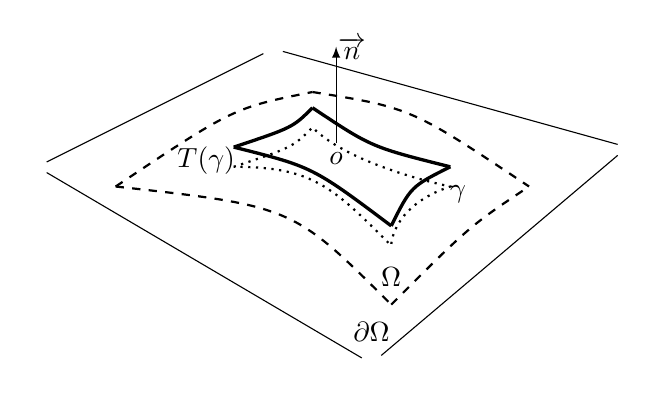
\begin{tikzpicture}[scale = 0.5]
\draw[dashed,thick] (-7.5,-1.5).. controls (-3,-2) and (-3,-2) .. (-0.5,-4.5);
\draw[dashed,thick](-0.5,-4.5) .. controls (1.5,-2.5) and (1.5,-2.5) .. (3,-1.5);
\draw[dashed,thick] (-7.5,-1.5) .. controls (-4.5,0.5) and (-4.5,0.5) .. (-2.5,0.9);
\draw[dashed,thick] (-2.5,0.9) .. controls (0,0.5) and (0,0.5) .. (3,-1.5);
\node (v1) at (-3.5,2) {};
\node (v4) at (-9.5,-1) {};
\node (v3) at (-1,-6) {};
\node (v2) at (5.5,-0.5) {};
\draw  (v1) edge (v2);
\draw  (v2) edge (v3);
\draw  (v3) edge (v4);
\draw  (v4) edge (v1);
\draw [dotted,thick](-4.5,-1) .. controls (-3,-0.5) and (-3,-0.5) .. (-2.5,0) .. controls (-1.5,-1) and (1,-1.5) .. (1,-1.5) .. controls (-0.5,-2) and (-0.5,-3) .. (-0.5,-3) .. controls (-2,-1.5) and (-2.5,-1) .. (-4.5,-1);
\node at (-2,-1) {};
\node (v5) at (-1.9,-0.8) {$o$};
%\draw[] at (-2,-1) ;
\draw[very thick] (-4.5,-0.5) .. controls (-2.5,-1) and (-2.5,-1) .. (-0.5,-2.5) ;
\draw[very thick]  (-0.5,-2.5) .. controls (0,-1.5) and (0,-1.5) .. (1,-1);
\draw [very thick] (1,-1) .. controls (-1,-0.5) and (-1,-0.5) .. (-2.5,0.5);
\draw  [very thick](-2.5,0.5) .. controls (-3,0) and (-3,0) .. (-4.5,-0.5);
\node at (-0.5,-3.8) {$\Omega$};
\node at (-1,-5.2) {$\partial \Omega$};
\node at (1.2,-1.7) {$ \gamma$};
\node at (-5.2,-0.83) {$ T(\gamma)$};
\node at (-2,-1) {};
\node (v6) at (-1.9,2.3) {};
\draw[-latex]  (v5) edge (v6);
\node at (-1.5,2) {$\overrightarrow{n}$};
\end{tikzpicture}}
	\qquad
    \subfloat[]{            
\tikzmath{\dR=1.9;\da=-10.0;\dT=-0.59;\dD=-27.; \dV=-9.00;
\ra=7.5; \rb = \ra+\dR;
\rc=10.4; \rd = \rc+\dR;
\re=15.2; \rf = \re+0.1*\dR;
\rg=9.5; \rh = \rg+\dR;
\LNwee=0.5;
\LTree=1.3;
}

\begin{tikzpicture}[angle/.style={black,thick},]
\tdplotsetmaincoords{0}{10};
\pgfplotsset{every axis/.append style={
		%view={-30*(0*1)}{-30*(-3)},
		%view={-90}{-30*0},
		scale=1.1,
		axis lines=center,
		%axis on top,
		%xlabel={$y$},
		%ylabel={$x$},
		%zlabel={$z$},
               %axis x line=middle,    % put the x axis in the middle
               %axis y line=middle,    % put the y axis in the middle
                %axis z line=middle,    % put the z axis in the middle
               %axis line style={-stealth}, % arrows on the axis
               axis line style={draw=none},
               axis equal image,
,
            }}
    \pgfplotsset{ticks=none};
    \pgfplotsset{compat=1.12};
	\begin{axis}[]
			
		%*******************************    first geodesics  ***********************************
		\addplot [dashed,thin,decoration={markings, mark = at position 0.5 with {\arrow[scale = 2.5]{latex[reversed]}}},postaction ={decorate},samples=40,	samples y=0,	domain=90.0+10:0-10]
		({-4.5+\ra*cos(x)},{-4.5+\ra*sin(x)})node[above,left] {$\gamma_{1}$};
		
		
      		\def \f{19.6}%********************************************
      		\def\fe{-2}
	
      		\def \fff{77.2}%********************************************
	
  		%second geodesics **************************************
  			
		\addplot [dashed,thin,decoration={markings, mark = at position 0.6 with  {\arrow[scale = 2.5]{latex[reversed]}}},postaction ={decorate},samples=40,	samples y=0,	domain=300+80:295]({-9.1+\rg*cos(x)},{10+\rg*sin(x)})node[below,left,{anchor=north west}] {$\gamma_{2}$};
		
		\def\qt{2.55};
	
      		
      		
  		\def\mbt{-49};
  		
 		%***************************                           third geodesics                 *********************************
 		
		\addplot [dashed,thin,decoration={markings, mark = at position 0.5 with {\arrow[scale = 2.5]{latex[reversed]}}},postaction ={decorate},samples=40,	samples y=0,	domain=0-35:70.0+45]({\rc*cos(x)},{\rc*sin(x)})node[below,left] {$\gamma_{3}$};
		
		\def\w{-15};
	
  		\def\ww{88};
			
  		%************************************************ fourth geodesics **************************************
  				
		\addplot [dashed,thin,decoration={markings, mark = at position 0.5 with {\arrow[scale = 2.5]{latex[reversed]}}},postaction ={decorate},samples=40,	samples y=0,	domain=270.0+20:270.0-30]({5-\re*cos(x)},{-17-\re*sin(x)})node[below,left] {$ \gamma_{4} \ $};
		
		\def\q{109.5};
 		
  		\def\mb{81};
		
    
%********************* angles between the 4 geodesic paths
				% ***************************** 1 and 4 *************************
					
	  	\draw[-Latex,black,  thin] let
   		 \p0 = ({-4.5+\ra*cos(\f)},{-4.5+\ra*sin(\f)}),
    		\p1 =   ({5+\re*cos(\mb+\dV)},{-17+1.1*\re*sin(\mb+\dV)}) ,
    		\p2 =  ({-4.5+\ra*cos(\f-\da)},{-4.5+\ra*sin(\f-\da)}),
    		\n1 = {atan2(\y1 - \y0,\x1 - \x0)},
    		\n2 = {atan2(\y2 - \y0,\x2 - \x0)},
    		\n3 = {0.6cm},
    		\n4 = {(\n1 + \n2) / 2}
  		in ({-4.5+\ra*cos(\f)},{-4.5+\ra*sin(\f)}) +(\n1:\n3) arc[radius = \n3, start angle = \n1, end angle = \n2]node[midway,{anchor=south}] {$\ \ \Psi_{4\rightarrow 1}$};;
				
				% ***************************** 1 and 2 *************************
					
	  	\draw[-Latex,,black,  thin] let
   		\p0 = ({-4.5+\ra*cos(\fff)},{-4.5+\ra*sin(\fff)}),
    		\p1 =   ( {-4.5+\ra*cos(\fff+\da)},{-4.5+\ra*sin(\fff+\da)}),
    		\p2 =({-9.1+\rg*cos(\mbt-\dD)},{10+1.19*\rg*sin(\mbt-\dD)}),
    		\n1 = {atan2(\y1 - \y0,\x1 - \x0)},
    		\n2 = {atan2(\y2 - \y0,\x2 - \x0)},
    		\n3 = {0.65cm},
    		\n4 = {(\n1 + \n2) / 2}
  		in ({-4.5+\ra*cos(\fff)},{-4.5+\ra*sin(\fff)}) +(\n1:\n3) arc[radius = \n3, start angle = \n1, end angle = \n2]node[midway,right]{$\Psi_{1\rightarrow 2}$};		
				
				% ***************************** 2 and 3  *************************
		 \draw[-Latex,black,  thin] let
   		 \p0 = ({\rc*cos(\ww)},{\rc*sin(\ww)}),
    		\p1 =   ({-9.1+1.1*\rg*cos(\qt+\dD)},{10+1.1*\rg*sin(\qt+\dD)}) ,
    		\p2 =  ({\rc*cos(\ww+\dT)},{\rc*sin(\ww+\dT)}),
    		\n1 = {atan2(\y1 - \y0,\x1 - \x0)},
    		\n2 = {atan2(\y2 - \y0,\x2 - \x0)},
    		\n3 = {0.8cm},
    		\n4 = {(\n1 + \n2) / 2}
  		in ({\rc*cos(\ww)},{\rc*sin(\ww)}) +(\n1:\n3) arc[radius = \n3, start angle = \n1, end angle = \n2]node[midway,right ] {$\  \ \Psi_{2\rightarrow 3}$};	
			
			
						% ***************************** 3 and 4  *************************
		 \draw[-Latex,black,  thin] let
   		 \p0 = ({\rc*cos(\w)},{\rc*sin(\w)},0),
    		\p1 =  ({\rc*cos(\w+\dT)},{1.04*\rc*sin(\w+\dT)}),
    		\p2 =({5-\rf*cos(\q-\dV)},{-17+\rf*sin(\q-\dV)}),
    		\n1 = {atan2(\y1 - \y0,\x1 - \x0)},
    		\n2 = {atan2(\y2 - \y0,\x2 - \x0)},
    		\n3 = {-0.8cm},
    		\n4 = {(\n1 + \n2) / 2}
  		in ({\rc*cos(\w)},{\rc*sin(\w)}) +(\n1:\n3) arc[radius = \n3, start angle = \n1, end angle = \n2]node[midway,{anchor=south}] {$ \Psi_{3\rightarrow 4} \ \ \ \ \ $};	
		\draw[very  thick]({\rc*cos(\w)},{\rc*sin(\w)},)-- ({\rc*cos(\ww)},{\rc*sin(\ww)});
		\draw[very  thick]({-4.5+\ra*cos(\fff)},{-4.5+\ra*sin(\fff)})-- ({\rc*cos(\ww)},{\rc*sin(\ww)});
		\draw[very  thick]({-4.5+\ra*cos(\fff)},{-4.5+\ra*sin(\fff)})-- ({-4.5+\ra*cos(\f)},{-4.5+\ra*sin(\f)});
		\draw[very thick]({\rc*cos(\w)},{\rc*sin(\w)})-- ({-4.5+\ra*cos(\f)},{-4.5+\ra*sin(\f)});
		
		\def \fet{-0.27};
 		\draw[thick, -Latex]({-9.1+\rg*cos(\mbt)},{10+\rg*sin(\mbt)}) -- ({(1-\fet)*(-9.1+\rg*cos(\mbt))+\fet*(-9.1+\rg*cos(\mbt+\dD))},{(1-\fet)*(10+\rg*sin(\mbt))+\fet*(10+1.2*\rg*sin(\mbt+\dD))})node[below,right] {};
 		\def\fe{1}
 		 \draw[thick, -Latex]({-4.5+\ra*cos(\fff)},{-4.5+\ra*sin(\fff)},0) -- ({(1-\fe)*(-4.5+\ra*cos(\fff))+\fe*(-4.5+\ra*cos(\fff+\da))},{(1-\fe)*(-4.5+\ra*sin(\fff))+\fe*(-4.5+\ra*sin(\fff+\da))},0)node[{anchor=south west}]  {};		
  		  
		  \node[{anchor=north east}]  at ({-4.5+\ra*cos(\f)},{-4.5+\ra*sin(\f)}){$p_1$};
		 \node[{anchor=south east}]  at ({-4.5+\ra*cos(\fff)},{-4.5+\ra*sin(\fff)}){$p_2$};
		  \node[{anchor=south east}]  at ({\rc*cos(\ww)},{\rc*sin(\ww)}){$p_3$};
		   \node[{anchor=south west}]  at ({\rc*cos(\w)},{\rc*sin(\w)}){$p_4$};
  		 \draw[Latex-,black,  thin] let
   		 \p0 = ({-4.5+\ra*cos(\fff)},{-4.5+\ra*sin(\fff)}),
    		\p1 =   ({\rc*cos(\ww)},{\rc*sin(\ww)}),
    		\p2 =({-4.5+\ra*cos(\f)},{-4.5+\ra*sin(\f)}),
    		\n1 = {atan2(\y1 - \y0,\x1 - \x0)},
    		\n2 = {atan2(\y2 - \y0,\x2 - \x0)},
    		\n3 = {1.7cm},
    		\n4 = {(\n1 + \n2) / 2}
  		in({-4.5+\ra*cos(\fff)},{-4.5+\ra*sin(\fff)}) +(\n1:\n3) arc[radius = \n3, start angle = \n1, end angle = \n2]node[midway,right ] {$\nu_{2}$};	
		
  		
  		
\end{axis}
\end{tikzpicture}}
\caption{Relationship between parallel transportation along a closed path and the excess of the angle-sum over four right angles of a quadrilateral.}
\label{fig:fig_p96_3415_d}
\end{figure}\\
\\ Let's look at the point $p_2$ on $\partial \Omega$. We have $\nu_2 = \epsilon^{-}+\Psi_{1 \rightarrow 2} +\epsilon^{+}= \Psi_{1 \rightarrow 2}+\epsilon$. In general,
\begin{align}
\sum_{i=1}^{4} \nu_i &= 2\pi \\
\underbrace{\sum_{i=1}^{4} \Psi_{i \rightarrow i+1}}_{= - \delta \theta} +\sum_{i=1}^{4} \epsilon_{i} &= \sum_{i=1}^{4} \frac{\pi}{2} \\
\Rightarrow \quad - \delta \theta &= \sum_{i=1}^{4}(\frac{\pi}{2} - \epsilon _{i})
\end{align}
Calling $\frac{\pi}{2} - \epsilon _{i}$ the excess, we get the assertion made.

$$\blacklozenge$$
\newpage

\section{p98 - Clarification}
\begin{tcolorbox}
... it is easy to see that the expansion takes the form $$\mathbf{3.425.}\spatie  \eta=\theta\left(s-\frac{1}{6}\epsilon K s^3 + \dots\right)$$
\end{tcolorbox}
Expanding $\eta$ in a power series gives
\begin{align}
\eta &= \underbrace{\left.\eta\right|_0}_{=0} + \underbrace{\left.\dv{\eta}{s}\right|_0 }_{=\theta}s -\half\underbrace{\left.\dv[2]{\eta}{s}\right|_0}_{=0}s^2 + \frac{1}{6}\left.\dv[3]{\eta}{s}\right|_0s^3 + \dots \\ 
\dv[2]{(1)}{s} \quad \Rightarrow\quad \dv[2]{\eta}{s} &=\left.\dv[3]{\eta}{s}\right|_0s+ \dots\\
\text{for } \lim_{ s \to 0} \ \text{ we have } \eta \approx \theta s \quad \text{so (2)} \quad \Rightarrow\quad \dv[2]{\eta}{s} &=\left.\dv[3]{\eta}{s}\right|_0\frac{\eta}{\theta}+ \dots\\
\lim_{ s \to 0}\quad \Rightarrow \quad \left.\dv[3]{\eta}{s}\right|_0 &= \theta\underbrace{\lim_{ s \to 0}\frac{1}{\eta}\dv[2]{\eta}{s}}_{= -\epsilon K}\\
\Rightarrow \quad \eta&=\theta\left(s-\frac{1}{6}\epsilon K s^3 + \dots\right)
\end{align}
$$\blacklozenge$$
\newpage

\section{p102 - Clarification}
\begin{tcolorbox}
Still using the same notation and Fig. 7, we have at B the three vectors $(T^r)_1,\ (T^r)_2,\ Y_r$ ...  it follows that $$\textbf{3.516.}\quad \quad (\Delta T^r)_A(Y_r)_{A'2}= - (\Delta T^r)_B(Y_r)_B$$
\end{tcolorbox}
First we note that for an invariant "propagated parallely" along a curve we have $$\fdv{(T^r Y_r)}{u} = \fdv{T^r} {u}Y_r+T^r\fdv{Y_r}{u}=0$$
\begin{figure}[h]
\begin{tikzpicture}[scale=1.5]
\coordinate (v1) at (-4,-2) ;
\coordinate (v2) at (-4,-1) ;
\coordinate (v3) at  (0.5,2.5);
\coordinate (v4) at (-0.5,3) ;
\coordinate (v4t) at (-3,3) ;
\coordinate (v5) at  (0.5,2.5) ;
\coordinate (v6) at (1,3.5);
\coordinate (v7) at (0.5,4.5) ;
\coordinate (v8) at (-2.4,-0.9)  ;
\coordinate  {} ;
\coordinate (A) at (-4,-2);
\node[{anchor = north west}] at (v1){$A$};
\node[{anchor = north west}] at (v3){$B$};
%\draw[black,fill] (v1) circle (1pt);
%\draw[black,fill] (v3) circle (1pt);
\draw [ thick](v1) .. controls (-0.5,-1) and (0,-1) .. (v3) ;
\draw [ thick] (v1) .. controls (-2.5,1) and (-2.5,1) .. (v3);
\node[{anchor=south east}] at (v2)  {$(T^r)_0$};
\draw[-latex, ultra thick]  (v1) edge (v2);
\node[{anchor=south west}]  at (v4t) {$(T^r)_2 = (T^r)_1+(\Delta T^r)_B $};
\draw[-latex, ultra thick] (v3) edge (v4);
\node[{anchor=south west}]  at (v6) {$(T^r)_1$};
\draw[-latex,ultra thick]  (v5) edge (v6);
\draw [dashed, thin, decoration={markings, mark = between positions 0.45 and 0.55 step 2em with { \arrow[scale = 2.0]{Latex[]}}},postaction ={decorate}](-4,-1) .. controls (-1.5,0) and (-1.5,0) .. (-0.5,3);
\draw [loosely dotted, thin, decoration={markings, mark = between positions 0.25 and 0.35 step 2em with { \arrow[scale = 2.0]{Latex[reversed,open]}}},postaction ={decorate}](-4,-1) .. controls (-1.5,0) and (-1.5,0) .. (-0.5,3);
\draw  [loosely dashdotted,   thin, decoration={markings,  mark = at position 0.5 with {\arrow[scale = 2.]{Latex[]}}},postaction ={decorate}] (-4,-1) .. controls (-3,1.5) and (-2,2) .. (1,3.5);
%\draw  [loosely dashdotted, ultra  thick, decoration={markings,  mark = between positions 0.5 and 0.58 step 3em  with {\arrow[scale = 1.5]{Latex[]}}},postaction ={decorate}] (-4,-1) .. controls (-3,1.5) and (-2,2) .. (1,3.5);

\draw[-latex, ultra thick]  (v3) edge (v7);
\draw[-latex, ultra thick]  (A) edge (v8);
%\draw[-latex, ultra thick]  (A) edge (v9);
\node[{anchor=south west}]  at (v7) {$(Y_r)_B$};
\node[{anchor=north west}]  at (v8) {$(Y_r)_{A,2}$};
%\node[{anchor=north east}]  at (v9) {$(Y_r)_{A,1}$};
%\draw[loosely dashed, ultra thick, decoration={markings, mark = at position 0.5 with {\arrow[scale =1.5]{Latex[open]}}},postaction ={decorate}] (v7) .. controls (-3.5,3) and (-3.5,3) .. (v9);
\draw[loosely dashed,thin,decoration={markings, mark = between positions 0.45 and 0.55 step 2em with {\arrow[scale = 2.0]{Latex[open]}}},postaction ={decorate}] (v7) .. controls (-0.5,-0.5) and (-0.5,0) .. (v8);
\coordinate (u1) at (-2,0.8) ;
\coordinate (u2) at (-1,-1)  ;
\node[{anchor=south west}]  at (u1) {$C_1$};
\node[{anchor=north west}]  at (u2) {$C_2$};
\coordinate (t1) at (-5,-2);
\coordinate (t2) at (-4.5,-3);
%\node[{anchor=south east}]  at (t1) {$(T^r)_{21}$};
\node[{anchor=north west}]  at (t2)  {$(T^r)_{0}+ (\Delta T^r)_A$};
%\draw[-latex, ultra thick]  (A) edge (t1);
\draw[-latex, ultra thick]  (A) edge (t2);
%\draw[-latex, ultra thick, dashed]   (t1) edge (t2);

%\draw[-latex, ultra thick, dashed]   (v2) edge (t1);
%\coordinate(t3) at (-5,-2.5) {} {};
%\node[{anchor=north east}]  at (t3) {$(\Delta T^r)_{A}$};
%\draw[dashed, ultra thick, decoration={markings, mark = between positions 0.45 and 0.55 step 2em with {\arrow[scale = 1.5]{Latex[]}}},postaction ={decorate}] (-0.5,3) .. controls (-2,2.5) and (-4,1) .. (-5,-2);
\draw [loosely dashdotted, thin, decoration={markings, mark = between positions 0.5 and 0.57step 2em with {\arrow[scale = 2.0]{Latex[open]}}},postaction ={decorate}] (1,3.5) .. controls (1,-2) and (0,-1.5) .. (-4.5,-3);

%\coordinate(t4) at (-4.2,-1.7);
%\node[{anchor=north east}]  at (t4) {$(\Delta T^r)_{A}$};
\draw[dotted]  plot[smooth cycle, tension=.7] coordinates {(0,4.5)  (0.5,3.5) (1.5,3) (2.5,3.5) (1.5,4) (1.5,4.5) (1,5) (0.5,5)  (0,5)};
\draw[dotted]  plot[smooth cycle, tension=.7] coordinates {(-5,-3) (-5,-3.5) (-4.5,-3.5) (-4,-3.5) (-3,-3.5) (-2.5,-3) (-3,-2.5) (-3.5,-2.5) (-1.5,-1.5) (-2,-0.5) (-3,-1) (-4.5,-2) (-4.5,-2.5)};
\draw[dashed,very thin]  plot[smooth cycle, tension=.7] coordinates {(-5.5,-1) (-5,-1.5) (-3.5,-1.5) (-3,-1.5) (-1.5,-1.5) (-1.5,-0.5) (-2.5,0) (-3.5,0) (-4.5,0) (-5.5,-0.5) (-5.5,-1)};
\draw[dashed,very thin]  plot[smooth cycle, tension=.7] coordinates {(-2.5,2.5)   (-1.5,2.5) (0,2.5) (0.5,3) (1,4) (1.5,5.5) (0.5,5.5) (0,4) (-0.5,3.5) (-3,3.5) (-3.5,3) };
\coordinate (z1) at (-2.5,-3.5) {};
\coordinate (z2) at (2,3) {};
\coordinate (z3) at (-5,0) ;
\coordinate (z4) at (-3.2,2.4) ;
\node[{anchor=south west}]  at (z1)  {$(4)$};
\node[{anchor=north east}]  at (z2)  {$(4)^{'}$};
\node[{anchor=south west}]  at (z3)  {$(3)$};
\node[{anchor=south east}]  at (z4)  {$(3)^{'}$};
\end{tikzpicture}\\
\caption{Parallel transportation along a  closed path}
\label{fig:fig_p102_3516_a}
\end{figure}
In fig. ~\ref{fig:fig_p102_3516_a} we use the following convention:\\
- a one black arrowed line means a forward propagation from $A$ to $B$ along $C_1$\\
- a double black arrowed line means a forward propagation from $A$ to $B$ along $C_2$\\
- a double open arrowed line means a backward propagation from $B$ to $A$ along $C_2$\\\\
In order to find the angular displacement of the vector $(T^r)_0$ when propagated parallely from $A$ to $B$ and back to $A$ along different paths, we follow  the dash dotted line in Fig. 1.7. Following that path, we end with the vector $(T^r)_0+ (\Delta T^r)_{A})$ in $A$ and have the vector $(T^r)_1$ as intermediate forward propagation from $A$ to $B$ along $C_1$, that vector being transported backwards to $A$ along $C_2$.\\\\
Note that for a vector the forward and backward propagation along the same curve is a null operation:$$(T^r)_0 \underset{\underset{C_2}{A\rightarrow B}}{\rightarrow} (T^r)_2 \underset{\underset{C_2}{B\rightarrow A}}{\rightarrow} (T^r)_0$$
Also, we have in Fig.1.7.
$$(T^r)_0 \underset{\underset{C_1}{A\rightarrow B}}{\rightarrow} (T^r)_1 \underset{\underset{C_2}{B\rightarrow A}}{\rightarrow} (T^r)_0+ (\Delta T^r)_{A}$$
$$(Y_r)_{B} \underset{\underset{C_2}{B\rightarrow A}}{\rightarrow} (Y_r)_{A,2}$$
At $A$ we form the following invariants
\begin{align}
\left \{ \begin{array}{l}
 ((T^r)_0+ (\Delta T^r)_{A})\ (Y_r)_{A,2}\\
 (T^r)_0 \ (Y_r)_{A,2}
\end{array} \right.
\end{align}\\
and at $B$
\begin{align}
\left \{ \begin{array}{l}
 (T^r)_1\ (Y_r)_{B}\\
 (T^r)_2 \ (Y_r)_{B} = ((T^r)_1+(\Delta T^r)_B )\ (Y_r)_{B}
\end{array} \right.
\end{align}\\

Due to the null effect of  parallel propagation on invariants, we  get
\begin{align}
 (T^r)_1\ (Y_r)_{B} &= ((T^r)_0+ (\Delta T^r)_{A})\ (Y_r)_{A,2}\\
 ((T^r)_1+(\Delta T^r)_B )\ (Y_r)_{B}&=(T^r)_0 \ (Y_r)_{A,2}\\
 \text{(3)-(4)}\quad \Rightarrow \quad -(\Delta T^r)_B )\ (Y_r)_{B}&=(\Delta T^r)_{A})\ (Y_r)_{A,2}
\end{align}\\
$$\blacklozenge$$
\newpage


\section{p105 - Clarification}
\begin{tcolorbox}
\begin{align*}
\textbf{3.521.} \spatie \dv{I}{v} &= \int_{u_1}^{u_2}\partial_v\left(T_n\partial_u x^n\right)du\\
&= \int_{u_1}^{u_2}\fdv{T_n}{v}\partial_u x^n du + \int_{u_1}^{u_2}T_n\fdv{\left(\partial_u x^n\right)}{v} du. 
\end{align*}
Now $\fdv{T_n}{v}=0$, since $T_r$ is propagated along $\textit{all}$ curves in $V_n$.
\end{tcolorbox}
To better understand this last statement recall that from 3.515, we have
\begin{align*}
 \left( \Delta T^r \right)_B \left( Y_r \right)_B &= \int \int Y_rR^r_{.pmn}T^p\partial _u x^m \partial _v x^n du dv\\
 &= 0 \quad \text{as} \spatie R^r_{.pmn}=0
\end{align*}
As $\left( Y_r \right)_B$ is arbitrary we have $\left( \Delta T^r \right)_B =0$. Consider fig. ~\ref{fig:fig_p105_3521_a} below.\\
\begin{figure}[H]
\center
\begin{tikzpicture}[scale=1.3]
\coordinate (v1) at (-4,-2) ;
\coordinate (v2) at (-4,-1) ;
\coordinate (v3) at  (0.5,2.5);
\coordinate (v4) at (0.5,3.5) {} ;
\coordinate  {} ;
\coordinate (A) at (-4,-2);
\node[{anchor = north east}] at (v1){$A$};
\node[{anchor = north west}] at (v3){$B$};
%\draw[black,fill] (v1) circle (1pt);
%\draw[black,fill] (v3) circle (1pt);
\draw [ thick](v1) .. controls (-0.5,-1) and (0,-1) .. (v3) ;
\draw [ thick] (v1) .. controls (-2.5,1) and (-2.5,1) .. (v3);
\node[{anchor=south east}] at (v2)  {$(T^r)_A$};
\draw[-latex, ultra thick]  (v1) -- (v2);
\node[{anchor=south west}]  at (v4)  {$(T^r)_B$};;
\draw[-latex, ultra thick] (v3) -- (v4);
\coordinate (p1) at (-3,-0.1) {};
\coordinate (p1a) at (-3,1.0) {};
\coordinate (p1at) at (-3.2,1.1) {};
\coordinate (p2) at (-2.5,-1.57) {};
\coordinate (p2a) at (-2.5,-0.5) {};
\draw[black,fill] (p1) circle (1pt);
\draw[black,fill] (p2) circle (1pt);
\draw[-latex, ultra thick]   (p1) -- (p1a);
\draw[-latex, ultra thick]   (p2) -- (p2a);
\node[{anchor=south west}] at (p1at)  {$(T^r)_{u, v+dv}$};
\node[{anchor=south west}] at (p2a)  {$(T^r)_{u,v}$};
\node[{anchor=north west}] at (p2)  {$P$};
\node[{anchor=north west}] at (p1)  {$P^{'}$};
\draw [loosely dashdotted,   ultra thick, decoration={markings,  mark = at position 0.5 with {\arrow[scale = 0.8]{Latex[]}}},postaction ={decorate}](A) .. controls (-3,-2) and (-3,-2) .. (p2);
\draw[loosely dashdotted,   ultra thick, decoration={markings,  mark = at position 0.5 with {\arrow[scale = 0.8]{Latex[reversed]}}},postaction ={decorate}] (p1) .. controls (-3,-1) and (-3,-1) .. (p2);
\end{tikzpicture}\\
\caption{Parallel transportation along a path in a space with zero curvature tensor}
\label{fig:fig_p105_3521_a}
\end{figure}
Consider the path $A\rightarrow P \rightarrow P^{'}$, $ P$ being situated at the parametric coordinates $(u, v)$ and $P^{'}$ at $(u, v + dv)$. For this path we have also $\left( \Delta T^r \right)_{P,P^{'}} =0$. So $(T^r)_{u,v} = (T^r)_A$ and $(T^r)_{u,v+dv} = (T^r)_{u,v}$ and thus $\fdv{T_r}{v}=0$.
$$\blacklozenge$$
\newpage

\section{p108 - Exercise 1}
\begin{tcolorbox}
Taking polar coordinates on a sphere of radius a, calculate the curvature tensor, the Ricci tensor, and the curvature invariant.
\end{tcolorbox}
We have 
\begin{align}
 \Phi = a^2d\theta^2 + a^2\sin^2 \theta d\phi^2
\end{align}
We only have to calculate $R_{1212}$ (see exercise page 86).
\begin{align}
 R_{\theta\phi\theta\phi}&= \partial_{\theta}\underbrace{[\phi \phi,\theta]}_{= -a^2\sin\theta\cos\theta} -\partial_{\phi}\underbrace{[\phi \theta,\theta]}_{=0} + \underbrace{\Gamma^{\theta}_{\phi\theta}}_{=0}[\theta\phi,\theta]+ \underbrace{\Gamma^{\phi}_{\phi\theta}[\theta\phi,\phi]}_{=a^2\cos^2\theta} - \underbrace{\Gamma^{\theta}_{\phi\phi}}_{=0}[\theta\theta,\theta]- \underbrace{\Gamma^{\phi}_{\phi\phi}}_{=0}[\theta\theta,\phi]\\
 &= a^2\sin^2\theta\\
 \text{3.208. : }& \quad \frac{R_{11}}{a_{11}}=\frac{R_{22}}{a_{22}}=-\frac{R_{\theta\phi\theta\phi}}{det(a_{mn})}\quad\Rightarrow \quad \left \{ \begin{array}{l}
 R_{11} =  -1\\
 R_{12} = 0\\
 R_{22} =  -\sin^2\theta
\end{array} \right.\\
\text{3.210. : }& \quad R=-\frac{2}{det(a_{mn})}R_{\theta\phi\theta\phi}\quad\Rightarrow \quad R= -\frac{2}{a^2}
\end{align}
$$\blacklozenge$$
\newpage

\section{p108 - Exercise 2}
\begin{tcolorbox}
Take as manifold $V_2$ the surface of an ordinary right circular cone, and consider one of the circular sections. A vector in $V_2$ is propagated parallely round this circle. Show that its direction is changed on completion of the circuit. Can you reconcile this result with the fact that $V_2$ is flat?
\end{tcolorbox}
\begin{figure}[h]
\center
\pgfplotsset{every axis/.append style={
		view={-30*1}{-20*1},
		%view={-90}{-30*0},
		scale=1.5,
		axis lines=center,
		axis on top,
		%xlabel={$x$},
		%ylabel={$y$},
		%zlabel={$z$},
		zmax=42,
		%xmin=-6,
               axis x line=middle,    % put the x axis in the middle
               axis y line=middle,    % put the y axis in the middle
                axis z line=middle,    % put the z axis in the middle
               %axis line style={-stealth}, % arrows on the axis
               %axis line style={draw=none}
            }}
           
\begin{tikzpicture}[angle/.style={black,thick},]
\tikzmath{\r=2.5;\h=5;\q=atan((\r/\h)); \kei=sin(\q);\skei=sqrt(\kei);\pr=0.549306/1 ; \pp=1.61557/2.5;};
\q, \h,\pr, \pp,\kei,\skei;
    \pgfplotsset{ticks=none};
    \pgfplotsset{compat=1.12};
	\begin{axis}
		[
		axis equal=true,
		]
		%draw the cylinder whiwh is tilted so that it 'rolls' on the x-y plane and oriented along the y-axis
		\addplot3 [surf,	dashed,thick,	mesh/interior colormap=
		{bw}{color=(gray!10) color=(gray!50)},
		colormap= {bw}{color=(black!10) color=(white!10)},
		domain=0:360,
		y domain=0:8.6*\h,
		samples=40,
		samples y=10,
		z buffer=sort,]
		({\y*tan(\q)*sin(x)},{\y*tan(\q)*cos(x)},{y});
	
		%add a base circle to emphasize the cone shape
		\addplot3 [black,thick,dotted,samples=40,	samples y=0,	domain=0.0:360,]({8.6*\h*tan(\q)*sin(x)},{8.6*\h*tan(\q)*cos(x)},{8.6*\h});
		\coordinate (O) at (0,0,0);
		\coordinate (V) at ({32*\kei*cos(30)},{32*\kei*sin(30)},32);
		\coordinate (Vp) at ({32*\kei*cos(30)},{32*\kei*sin(30)},0);
		\coordinate (Vp2) at ({50*\kei*cos(30)},{50*\kei*sin(30)},0);
		\coordinate (Vp3) at ({0},{0},32);
		\coordinate (Vp4) at ({0},{32*tan(\q)},32);
		\draw[-latex, thick] (O) -- (V);
		\draw[dashed] (V) -- (Vp);
		\draw[dashed] (Vp2) -- (O);
		\draw[dashed] (Vp3) -- (V);
		\draw[dashed] (Vp3) -- (Vp4);
		 \draw[-Latex,black] let
   		\p0 = (O) ,
    		\p1 =   (0,5,0) ,
    		\p2 =(Vp),
    		\n1 = {atan2(\y1 - \y0,\x1 - \x0)},
    		\n2 = {atan2(\y2 - \y0,\x2 - \x0)},
    		\n3 = {0.7cm},
    		\n4 = {(\n1 + \n2) / 3}
  		in (O) +(\n1:\n3) arc[radius = \n3, start angle = \n1, end angle = \n2]node[midway,below] {$\theta \ \ $};; 

 \draw[-Latex,black] let
   		\p0 = (Vp3) ,
    		\p1 =  (Vp4),
    		\p2 =(V),
    		\n1 = {atan2(\y1 - \y0,\x1 - \x0)},
    		\n2 = {atan2(\y2 - \y0,\x2 - \x0)},
    		\n3 = {0.4cm},
    		\n4 = {(\n1 + \n2) / 3}
  		in (Vp3) +(\n1:\n3) arc[radius = \n3, start angle = \n1, end angle = \n2]node[midway,below] {};;  
		%\draw[fill=black](O) circle(1.5pt)node[{anchor=northwest}] {$O$};  	
		\draw[fill=black](V) circle(0.5pt)node[{anchor=south west}] {$\mathbf{\overrightarrow{u}}$};  			
  		%add a  circle to emphasize the vector position
		\addplot3 [black,dashed,samples=40,	samples y=0,	domain=0.0:360,]({32*tan(\q)*sin(x)},{32*tan(\q)*cos(x)},{32});
		

\end{axis}
\end{tikzpicture}\\
\caption{Intrinsic coordinates on  a cone}
\label{fig:fig_p108_Ex2_a}
\end{figure}
We take as coordinate system $\left(u,\theta \right)$, embedded in the manifold, $u$ being the distance of the generator of the considered point to the apex of the cone and $\theta$ the angle with a arbitrary vector laying in a plane perpendicular to the axis of the cone.\\
It is not hard to see that the fundamental form for this manifold is $$ \Phi = du^2+ \underbrace{k}_{= \ \sin^2 \alpha}u^2 d\theta^2 $$ 
We have 
\begin{align*}
 (a_{mn})= \begin{pmatrix}
 1&0  \\
 0& k u^2 \\
\end{pmatrix}\quad
 (a^{mn})= \begin{pmatrix}
 1&0  \\
 0& \frac{1}{k u^2} \\
\end{pmatrix}\\
 \begin{pmatrix}
 \left[ mn,u \right] \\
 \left[ mn,\theta \right] \\
\end{pmatrix}=\begin{pmatrix}
 0&0&-k u \\
 k u&0&0 \\
\end{pmatrix}\\
 \begin{pmatrix}
 \Gamma^u_{mn} \\
 \Gamma^{\theta}_{mn} \\
\end{pmatrix}=\begin{pmatrix}
 0&0&-k u \\
 0&\frac{1}{u}&0 \\
\end{pmatrix}
\end{align*}

Let's calculate the curvature tensor. From the exercise on page 86 we know that for a $V_2$ all components of the curvature tensor can be expressed in terms of $R_{1212}$. We have
\begin{align*}
R_{u\theta u\theta} &= \left \{ \begin{array}{l}
\frac{1}{2}\left(\partial_{\theta u}a_{u \theta}+\partial_{u \theta}a_{\theta u}-\partial_{\theta \theta}a_{uu}-\partial_{u u}a_{\theta \theta}  \right) \\
 + a^{pq}\left([u \theta,p][\theta u,q] -[u u,p][\theta \theta,q]  \right)
\end{array} \right.
&= \left \{ \begin{array}{l}
-k \\
 + a^{uu}\left(\underbrace{[u \theta,u][\theta u,u] -[u u,u][\theta \theta,u]}_{=0}  \right)\\
 + \underbrace{a^{u \theta}}_{=0}\left([u \theta,u][\theta u,\theta] -[u u,u][\theta \theta,\theta]  \right)\\
 + \underbrace{a^{\theta u}}_{=0}\left([u \theta,\theta][\theta u,u] -[u u,\theta][\theta \theta,u]  \right)\\
 + \underbrace{a^{\theta \theta}}_{=\frac{1}{ku^2}}\left(\underbrace{[u \theta,\theta][\theta u,\theta]}_{= k^2u^2} -\underbrace{[u u,\theta][\theta \theta,\theta]}_{=0}  \right)\\
\end{array} \right.
\end{align*}
So indeed all components of the curvature tensor vanish and hence $V_2$ is flat.

Let's now calculate the parallel transportation of a vector $T^r$ along a circle somewhere on the cone. Taking $\theta$ as the parameter of the curve, the equation of the curve is $(u=u_0,\ \theta) \quad \theta \in \ \left[0, 2\pi \right)$. We have for parallel transportation along that curve $\fdv{T^r}{\theta}=0$ and get
\begin{align}
 & \left \{ \begin{array}{l}
\dv{T^u}{\theta} + \Gamma^u_{\theta \theta}T^{\theta}\dv{\theta}{\theta} =0\\\\
\dv{T^{\theta}}{\theta} + \Gamma^{\theta}_{u \theta}T^{u}\dv{\theta}{\theta}+ \Gamma^{\theta}_{\theta u}T^{\theta}\underbrace{\dv{u}{\theta}}_{=0} =0\quad \left(\dv{u}{\theta} = 0 \quad \text{as} \quad u= C^{st} \right)
\end{array} \right.\\
\Rightarrow \quad
 & \left \{ \begin{array}{l}
\dot{T^u} -ku_0 T^{\theta}=0\\\\
\dot{T}^{\theta} + \frac{1}{u_0}T^{u}=0
\end{array} \right.\\
\Rightarrow \quad
 & \left \{ \begin{array}{l}
\frac{\ddot{T}^u}{T^{u}} = -k\\\\
\dot{T}^{\theta} =- \frac{T^{u}}{u_0}
\end{array} \right.
\end{align}
From (3a) we deduce that a solution can be of the form\\ $T^u = p^{'}\left( e^{(a \theta + b^{'})}+ e^{-(a \theta + b^{'})}\right)$. Substituting in (3) we see that $a^2 = -k \rightarrow a = \pm i\sqrt{k}$. Replacing $b^{'}$ by $ib$ the solution for the system of differential equations (3) becomes
\begin{align}
T^u  &= p^{'}\left( e^{i(\sqrt{k} \theta + b)}+ e^{-i(\sqrt{k} \theta + b)}\right)\\
 &= p\cos{\left(\sqrt{k} \theta + b \right)}\\
 \Leftrightarrow \quad &=   C_1\sin{\sqrt{k}\theta}+ C_2\cos{\sqrt{k}\theta}\\
 \text{(6) in (3) gives:}\quad & \left \{ \begin{array}{l}
T^u = C_1\sin{\sqrt{k}\theta}+ C_2\cos{\sqrt{k}\theta}\\\\
T^{\theta}  =  \frac{1}{\sqrt{k}u_0}\left(C_1\cos{\sqrt{k}\theta}- C_2\sin{\sqrt{k}\theta}\right)\\
\end{array} \right.\\
\text{with} \quad & \left \{ \begin{array}{l}
 C_1=\sqrt{k}u_0\left.T^{\theta}\right|_{\theta=0} \\\\
 C_2=\left.T^{u}\right|_{\theta=0}\\
\end{array} \right.\\
\Rightarrow \quad & \left \{ \begin{array}{l}
T^u = \sqrt{k} u_0 T^{\theta}_{0}\sin{\sqrt{k}\theta}+ T^{u}_{0}\cos{\sqrt{k}\theta}\\\\
T^{\theta}  =   T^{\theta}_{0}\cos{\sqrt{k}\theta}- \frac{T^{u}_{0}}{\sqrt{k}u_0} \sin{\sqrt{k}\theta}\\
\end{array}\right.
\end{align}\\
Let's now compute the angle $\phi$ between the starting vector $T^r_{0}$ and the vector $T^r$ parallely transported over an angle $\theta$ on the circle. We have (see $\textbf{(2.301.)}$ and $\textbf{(2.312.)}$):
\begin{align*}
\left \{ \begin{array}{l}
 \left| T^r_0 \right|^2 =  \left(T^u_0\right)^2 + k u^2_0\left(T^{\theta}_0\right)^2\\\\
 \left| T^r \right|^2 =  \left(T^u_0\right)^2 + k u^2_0\left(T^{\theta}_0\right)^2\\\\
 \cos{\phi} =  \frac{T^u_0 T^u+k u^2_0T^{\theta}_0 T^{\theta} }{\left(T^u_0\right)^2 + k u^2_0\left(T^{\theta}_0\right)^2}
\end{array} \right.
\end{align*}
The last equation in (19) becomes
\begin{align*}
\cos{\phi} &= \cos{\sqrt{k}\theta} \\
\Rightarrow \quad \phi &= \sqrt{k}\theta + 2m\pi\quad\quad (m= 0,\pm 1,\pm 2, \dots)
\end{align*}
So for $\theta = 2\pi$ the angle between the starting vector and the transported vector is not $2m\pi$. 
\begin{figure}[H]%
    \centering
    \subfloat[]{\input{./images/fig_p108_Ex2_b1.tex}}
	\qquad
    \subfloat[]{\pgfplotsset{every axis/.append style={
		view={-30}{-30*1},
		%view={-90}{-30*0},
		scale=1,
		axis lines=center,
		axis on top,
		%xlabel={$x$},
		%ylabel={$y$},
		%zlabel={$z$},
               axis x line=none,    % put the x axis in the middle
               axis y line=middle,    % put the y axis in the middle
                axis z line=middle,    % put the z axis in the middle
               %axis line style={-stealth}, % arrows on the axis
               %axis line style={draw=none}
               %xaxis line style={draw=none}
            }}
 \begin{tikzpicture}[angle/.style={black,thick}]
\tikzmath{\r=1.5;\h=5;\q=asin((\r/\h)); \p=-\q*1 ; \k= \r/\h;};
\q, \h,\p, \k;
    \pgfplotsset{ticks=none};
    \pgfplotsset{compat=1.12};
\begin{axis}
		[
		axis equal=true,
		zmin=-\h*0,
		zmax=\r*1.2,
		]
			
		%draw the cylinder whiwh is tilted so that it 'rolls' on the x-y plane and oriented along the y-axis
		\addplot3 [surf,dashed,very thin,	mesh/interior colormap=
		{bw}{color=(gray!10) color=(gray!5)},
		colormap= {bw}{color=(black!10) color=(white!10)},
		domain=115:115+180,
		y domain=0:\h,
		samples=40,
		samples y=10,
		z buffer=sort,]
		({\y*cos(\p)+1*\y*tan(\q)*sin(x)*sin(\p)},{1*y*tan(\q)*cos(x)},{-\y*sin(\p)+1*\y*tan(\q)*sin(x)*cos(\p)});
		
		
		%draw the cylinder whiwh is tilted so that it 'rolls' on the x-y plane and oriented along the y-axis
		\addplot3 [surf,	dashed,thick,	mesh/interior colormap=
		{bw}{color=(gray!1) color=(gray!5)},
		colormap= {bw}{color=(black!1) color=(white!1)},
		domain=-65:115,
		y domain=0:\h,
		samples=40,
		samples y=10,
		z buffer=sort,]
		({\y*cos(\p)+1*\y*tan(\q)*sin(x)*sin(\p)},{1*y*tan(\q)*cos(x)},{-\y*sin(\p)+1*\y*tan(\q)*sin(x)*cos(\p)});

		%add a base circle to emphasize the cone shape
		\addplot3 [black,thick,dotted,samples=40,	samples y=0,	domain=0.0:360,]({\h*cos(\p)+1*\h*tan(\q)*sin(x)*sin(\p)},{1*\h*tan(\q)*cos(x)},{-\h*sin(\p)+1*\h*tan(\q)*sin(x)*cos(\p)});
		% add an arcsegment at 2/3 pf the cone
		\addplot3 [black,decoration={markings, mark = at position 0.5 with {\arrow[scale = 1.5]{latex[reversed]}}},postaction ={decorate},samples=40,	samples y=0,	domain=-5.0:-90,]({2*\h/3*cos(\p)+2*\h/3*tan(\q)*sin(x)*sin(\p)},{2*\h/3*tan(\q)*cos(x)},{-2*\h/3*sin(\p)+2*\h/3*tan(\q)*sin(x)*cos(\p)});%node[midway,right] {$x^1$};
		
 		
		%relevant points
		\coordinate (O) at ({ 0},{0},{0});%origin
		\coordinate (P) at ({ \h*1},{\h*0},{0});%point  P on the cone 

		\coordinate (A) at ({ \h*cos(\p)},{\h*0},{\h*sin(-\p)});
		\coordinate (Q) at ({1.* \h/cos(\p)},{\h*0},{0.*\h*sin(-\p)});

		%\node[tdplot_main_coords,{anchor=south west},red] at (P){$o$};
		%\draw[dashed,line width = 0.25mm] (O) --(P) ;%node[midway,right] {$x^1$};
		
		%\draw[dashdotted,line width = 0.25mm] (Q) --(A) ;%node[midway,right] {$x^1$};
		%draw points on cone
		\coordinate (W) at ({ \h/cos(\p)},{\h*0},{0.*\h*sin(-\p)});
		\coordinate (R) at ({2/3* \h/cos(\p)},{\h*0},{0.*\h*sin(-\p)});
		\coordinate (S) at ({2*\h/3*cos(\p)+2*\h/3*tan(\q)*sin(-5)*sin(\p)},{2*\h/3*tan(\q)*cos(-5)},{-2*\h/3*sin(\p)+2*\h/3*tan(\q)*sin(-5)*cos(\p)});
		\coordinate (T) at ({2*\h/3*cos(\p)+0*\h/3*tan(\q)*sin(-5)*sin(\p)},{0},{-2*\h/3*sin(\p)+0*\h/3*tan(\q)*sin(-5)*cos(\p)});
		\draw[fill=black](A) circle(0.5pt);%node[{anchor=north west}] {$A$};
		\draw[fill=black](Q) circle(0.5pt);%node[{anchor=north west}]{$A$};;
		\coordinate (Y) at ({\h*cos(\p)+\h*tan(\q)*sin(-5)*sin(\p)},{\h*tan(\q)*cos(-5)},{-\h*sin(\p)+\h*tan(\q)*sin(-5)*cos(\p)});
		\draw[fill=black](Y) circle(0.5pt);%node[{anchor=south east}] {$Y$};
		\draw[fill=black](W) circle(0.5pt);
		\draw[fill=black](R) circle(0.5pt)node[{anchor=north }] {$P$};
		\draw[-latex,dashed](O)--(R);
		\draw[fill=black](S) circle(0.5pt)node[{anchor=south east}] {$P_t$};
		\draw[fill=black](T) circle(0.5pt)node[{anchor=south west}] {};
		
		\coordinate (N) at ({1.14 *\h},{0},{0});
		\coordinate (Nt) at ({0.84 *\h},{0},{0});
		\draw[dotted,line width = 0.2mm] (O) --(Nt) ;
		\draw[dashdotted,- latex,black,line width = 0.25mm] (Nt) --(N) ;
		\coordinate (C) at ({1.2* \h*cos(\p)},{\h*0},{1.2*\h*sin(-\p)});
		\coordinate (Ct) at ({0.79* \h*cos(\p)},{\h*0},{0.79*\h*sin(-\p)});
		\draw[dotted,,line width = 0.2mm] (O) --(Ct) ;
		\draw[dashdotted,black,- latex,line width = 0.25mm] (Ct) --(C) ;
		
		\draw[- latex,line width = 0.25mm] (O) --(S) ;
		\draw[dashdotted,line width = 0.1mm] (T) --(R) ;
		\draw[dashdotted,line width = 0.1mm] (T) --(S) ;



		
		%projection onthe xy-plane
		%arcsegments of points P and R
		\begin{scope}
		\addplot3 [black,decoration={markings, mark = at position 0.5 with {\arrow[scale = 1.5]{latex}}},postaction ={decorate},samples=40,samples=40,	samples y=0,	domain=0:150,]
			({2/3*\h/cos(\q)*cos(x*sin(\q))},{2/3*\h/cos(\q)*sin(x*sin(\q))},{0});%node[midway,right] {$theta$};
		\end{scope}
		%projections  R*, P* of points R,P
		\coordinate (U) at ({2/3*\h/cos(\q)*cos(150*sin(\q))},{2/3*\h/cos(\q)*sin(150*sin(\q))},{0});
		\coordinate (V) at ({\h/cos(\q)*cos(150*sin(\q))},{\h/cos(\q)*sin(150*sin(\q))},{0});
		

		%\draw[dashdotted,line width = 0.25mm] (O) --(U) ;
		\draw[dashdotted,line width = 0.25mm] (O) --(V) ;
		
		%dots and labels of P* and R*
 		
 		\draw[fill=black](U)node[{anchor=north east}] {$P_t^{*}$};
 		\draw[- latex,line width = 0.25mm] (O) --(U) ;
 		%add labels of angles at a right place
 		 \coordinate (G) at({2/3*\h/cos(\q)*cos(90*sin(\q))},{2/3*\h/cos(\q)*sin(90*sin(\q))},{0});
 		\draw[](G) node[{anchor=north west}] {$\phi=\sqrt{k}\theta$};
 				
		\draw[dashdotted,line width = 0.1mm] (Y) --(S) ;
		\draw[dashdotted,line width = 0.1mm] (Y) --(A) ;
		\draw[dashdotted,line width = 0.1mm] (W) --(A) ;
 		\draw[-Latex,black,thin] let
   		\p0 = (A),
    		\p1 =  (Y),
    		\p2 =(W),
    		\n1 = {atan2(\y1 - \y0,\x1 - \x0)},
    		\n2 = {atan2(\y2 - \y0,\x2 - \x0)},
    		\n3 = {0.5cm},
    		\n4 = {(\n1 + \n2) / 2}
  		in (A) +(\n1:\n3) arc[radius = \n3, start angle = \n1, end angle = \n2]node[midway,below] {$\theta$};;
\end{axis}
\end{tikzpicture}}
\caption{Relationship between parallel transportation along a circle of a cone and unwrapping a cone .}
\label{fig:fig_p108_Ex2_b2}
\end{figure}
Fig. ~\ref{fig:fig_p108_Ex2_b2} illustrates the analogy between\\ 
(a): the $\parallel$ transportation of a vector $P$ along a circular curve $\gamma$ on the cone over an angle $\theta$ giving a vector $P_t$ making an angle $\phi = \sqrt{k}\theta$ with the starting vector, and \\
(b): the result of "unwrapping" a cone. Be two vectors $\overrightarrow{OP}$ and $\overrightarrow{OP_t}$, $P$ and $P_t$ being two points placed at a distance $r\theta$ along a circle  with radius $r$. Placing the vector $\overrightarrow{OP}$ in the $XY$-plane and unwrapping the cone over an angle $\theta$ will map the vector $\overrightarrow{OP_t}$ in the $XY$-plane to a vector $\overrightarrow{OP_t^{*}}$ making an angle $\phi = \sqrt{k}\theta$ with the vector $\overrightarrow{OP}$.\\
The transported vector will only coincide with the initial vector for $\sqrt{k}=\sin{\alpha}  = \frac{1}{n}\quad (n= 1, 2, \dots)$. Fig. ~\ref{fig:fig_p108_Ex2_b3} illustrates this in the $X-Y$-plane,  for n=3. Only after a transportation over three periods, will the transported vector coincide with the initial vector. The dotted area represents the unwrapped cone.
\begin{figure}[H]%
    \centering
{\begin{tikzpicture}[scale=0.5]
\tikzmath{%
  \r = 5.85;
}
\node (O) at (0,0) {};

\node (C1) at ({6*cos(0)},{6*sin(0)}) {};
\draw[](O)--(C1);
\node (C2) at ({6*cos(120)},{6*sin(120)}) {};
\draw[](O)--(C2);
\node (C3) at ({6*cos(2*120)},{6*sin(2*120)}) {};
\draw(O)--(C3);
\node (vC1) at ({4*cos(0)},{4*sin(0)}) {};
\draw[-latex,thick](O)--(vC1);
\node (vC2) at ({4*cos(120)},{4*sin(120)}) {};
\draw[-latex,thick](O)--(vC2);
\node (vC3) at ({4*cos(2*120)},{4*sin(2*120)}) {};
\draw[-latex,thick](O)--(vC3);
\draw  (O) circle (2pt);


\draw circle[dashed] [radius=\r];
\draw [black,pattern=dots, pattern color=gray]   (O) --  (-0.:\r) arc (0:120:\r) ;
\draw[black, dashed,very thin] circle (5.85cm);
\draw[black,thin] let
   \p0 = (O),
    		\p1 =  (C1),
    		\p2 =(C2),
    		\n1 = {atan2(\y1 - \y0,\x1 - \x0)},
    		\n2 = {atan2(\y2 - \y0,\x2 - \x0)},
    		\n3 = {2cm},
    		\n4 = {(\n1 + \n2) / 2}
  		in (O) +(\n1:\n3) arc[radius = \n3, start angle = \n1, end angle = \n2]node[midway,above] {$2\pi $};;
 
  \draw[black,thin] let
   		\p0 = (O),
    		\p1 =  (C2),
    		\p2 =(C3),
    		\n1 = {atan2(\y1 - \y0,\x1 - \x0)},
    		\n2 = {atan2(\y2 - \y0,\x2 - \x0)},
    		\n3 = {-2cm},
    		\n4 = {(\n1 + \n2) / 2}
  		in (O) +(\n1:\n3) arc[radius = \n3, start angle = \n1, end angle = \n2]node[midway,left,] {$4\pi$};;
  	\draw[-Latex,black,thin] let
  		   \p0 = (O),
    		\p1 =  (C3),
    		\p2 =(C1),
    		\n1 = {atan2(\y1 - \y0,\x1 - \x0)},
    		\n2 = {atan2(\y2 - \y0,\x2 - \x0)},
    		\n3 = {2cm},
    		\n4 = {(\n1 + \n2) / 2}
  		in (O) +(\n1:\n3) arc[radius = \n3, start angle = \n1, end angle = \n2]node[midway,below] {$6\pi$};;
\end{tikzpicture}}
\caption{Parallel transportation along a circle of a cone with $\sin{\alpha}  = \frac{1}{3}$ .}
\label{fig:fig_p108_Ex2_b3}
\end{figure}
$$\blacklozenge$$
\newpage

\section{p109 - Exercise 3 and 4}
$\mathbf{Exercise \ 3.}$\\
\begin{tcolorbox}
Consider the equations $$ \left( R_{mn} -\theta a_{mn}\right)X^n = 0$$ where $R_{mn}$ is the Ricci tensor in a $V_N \ (N>2)$, $\theta$ an invariant, and $X^n$ a vector. Show that, if these equations are to be consistent, $\theta$ must have one of a certain set of $N$ values, and that the vectors $X^n$ corresponding to different values of $\theta$ are perpendicular to one another. (The directions of these vectors are called the $\mathit{Ricci \ principal \ directions}$).
\end{tcolorbox}

\begin{align}
\left( R_{mn} -\theta a_{mn}\right)X^n = 0\\
 (1)\times (a^{mp}) \quad \Rightarrow \quad a^{mp} R_{mn}X^n  -\theta \underbrace{a^{mp}a_{mn}}_{=\delta^p_n}X^n  =0\\
 \Rightarrow \quad a^{mp} R_{mn}X^n  -\theta X^p  =0
\end{align}
Define $T^{p}_{n} =  a^{mp} R_{mn} $, then (3) can be written in matrix form with $\mathbf{T}\equiv (T^{p}_{n})$ , $\mathbf{X}\equiv (X^p)$ and $\mathbf{I} \equiv (\delta^i_j)$
\begin{align}
\left(\mathbf{T}-\theta \mathbf{I}\right)\mathbf{X} =0
\end{align}
This is an eigenvector equation with $\mathbf{T}$ being Hermitian i.e. $\mathbf{T}^{\dag} =\mathbf{T}$ . Indeed, obviously the complex conjugat $\mathbf{\overline{T}} = \textbf{T}$ and  
\begin{align*}
\mathbf{T}^T &=  \left(\mathbf{AR}\right)^T\\
 &= \mathbf{R}^T \mathbf{A}^T\\
 \Leftrightarrow \left(T^{j}_{i}\right)  &= \left(R_{kj}\right)^T\left(a^{ik}\right)^T\\
 &= \left(R_{jk}\right)\left(a^{ki}\right)
\end{align*}         
as both $ R_{jk}, \ a^{ki}$ are symmetric we  have
\begin{align*}
\left(T^{j}_{i}\right) &= \left(R_{kj}\right)\left(a^{ik}\right)\\
 &= \left(T^{i}_{j}\right)\\
 \Rightarrow \spatie \mathbf{T}^{\dag} &=\mathbf{T}
\end{align*} 
This means that the $N$ roots of $det\left(\mathbf{T}-\theta \mathbf{I_n}\right)=0$, which is a necessary condition to have equation (4) consistent, are real. Hence $\theta$ will take $N$ values, being the eigenvalues of the transformation matrix $\textbf{T}$. If all eigenvalues have multiplicity one, then  the N eigenvectors in (4) corresponding to the $N$ eigenvalues will be  orthogonal to each other. But, can eigenvalues with algebraic multiplicity $ m > 1$ occur? The answer is yes. Let's rewrite $P(\theta) = det\left(\mathbf{T}-\theta \mathbf{I_n}\right)$ as $\theta^{N} + q_i \theta^{n-i}  \quad (i= N-1,N-2,\dots, 1)$ with $q_i$ functions of the Ricci tensor components. The condition for eigenvalues with algebraic multiplicity $ m > 1$  to occur is that the determinant of the Sylvester matrix of the two following polynomial should be zero.
\begin{align}
\left \{ \begin{array}{l}
 P(\theta) = \theta^{N} + q_i \theta^{n-i}  \quad (i= N-1,N-2,\dots, 1)\\
 \dv{P(\theta)}{\theta} = N \theta^{N-1} + (n-i)q_i \theta^{n-i-1}  \quad (i= N-1,N-2,\dots, 1)
\end{array} \right.
\end{align}
The associated Sylvester matrix with these two polynomials will be of the form $$ S \left( P(\theta),\dv{P(\theta)}{\theta}\right) = \left( \begin{array}{cccccccc}
 1&q_{N-1}&\dots&q_1&0&0&\dots&0\\
 0&1&q_{N-1}&\dots&q_1&0&\dots&0\\
 \vdots&\vdots&\vdots&\vdots&\vdots&\vdots&\vdots&\vdots\\
 0&\dots&0&1&q_{N-1}&\dots &q_2&q_1\\
 N&(N-1)q_{N-1}&\dots&q_1&0&0&\dots&0\\
 0&N&(N-1)q_{N-1}&\dots&q_1&0&\dots&0\\
 \vdots&\vdots&\vdots&\vdots&\vdots&\vdots&\vdots&\vdots\\
 0&\dots&0&N&(N-1)q_{N-1}&\dots &2q_2&q_1\\
\end{array} \right)
$$
If the determinant of this matrix is not zero, then there will be no algebraic multiplicity. In the other case, one has to check whether in the eigenspace, related to the eigenvalues with algebraic multiplicity $ m > 1$, $m$ linear independent eigenvectors can be found.\\\\
$\mathbf{Exercise \ 4.}$
\begin{tcolorbox}
What becomes of the Ricci principal directions (see above) if $N=2$?
\end{tcolorbox}
From $\mathbf{3.208.}$ we have
\begin{align*}
\frac{R_{11}}{a_{11}} &= \frac{R_{12}}{a_{12}}=\frac{R_{22}}{a_{22}}=-\frac{R_{1212}}{a}\\
\Rightarrow\quad & \left \{ \begin{array}{l}
 T^{1}_{1} = a^{11}R_{11} +  a^{12}R_{21}\\
 T^{1}_{2} = a^{11}R_{12} +  a^{12}R_{22}\\
 T^{2}_{2} = a^{21}R_{12} +  a^{22}R_{22}\\
\end{array} \right.\\
\text{put } K=-\frac{R_{1212}}{a} \quad \Rightarrow\quad & \left \{ \begin{array}{l}
 T^{1}_{1} = K a^{11}a_{11} +  K a^{12}a_{12}\\
 T^{1}_{2} = Ka^{11}a_{12} +  Ka^{12}a_{22}\\
 T^{2}_{2} = Ka^{21}a_{12} +  Ka^{22}a_{22}\\
\end{array} \right.\quad
\Rightarrow\quad & \left \{ \begin{array}{l}
 T^{1}_{1} = K\delta^1_1 = K \\
 T^{1}_{2} = K\delta^1_2 = 0\\
 T^{2}_{2} = K\delta^2_2 = K\\
\end{array} \right.
\end{align*}
hence the characteristic equation $det\left(\mathbf{T}-\theta \mathbf{I_n} \right)=0$ becomes $ (K-\theta)^2=0$ . So only one value of $\theta$ exists as $\theta = K$.  Equation (4) becomes $\mathbf{0}\mathbf{X}=0$. So we can chose any pair of linear independent vectors as eigenvectors and can make them perpendicular to one another.
$$\blacklozenge$$
\newpage

\section{p109 - Exercise 5}
\begin{tcolorbox}
Suppose that two spaces $V_N$, $V^{'}_N$ have metric tensors $a_{mn}, \ a^{'}_{mn}$ such that $\ a^{'}_{mn}=k\ a_{mn}  $, where $k$ is a constant. Write down the relations between the curvature tensors, the Ricci tensors, and the curvature invariants of the two spaces.
\end{tcolorbox}
We have 
\begin{align*}
 ds^2 &= a_{mn}dx^{m} dx^{n}\\
 ds^{'2}&= a^{'}_{mn} dx^{'m}dx^{'n}
\end{align*}
But let's be careful: there is no reason to assume that  $dx^m = dx^{'m}$. Let's embed the two spaces in a space $V_{N+1}$. If an observer in that space sees two displacements  $ds^2$ and $ds^{'2}$ which for him have the same magnitude, we have
\begin{figure}[H]
\centering
\begin{minipage}[t]{.4\textwidth}
%\centering
\vspace{0pt}
%\includegraphics[scale=.5]{p85_ex1.png}
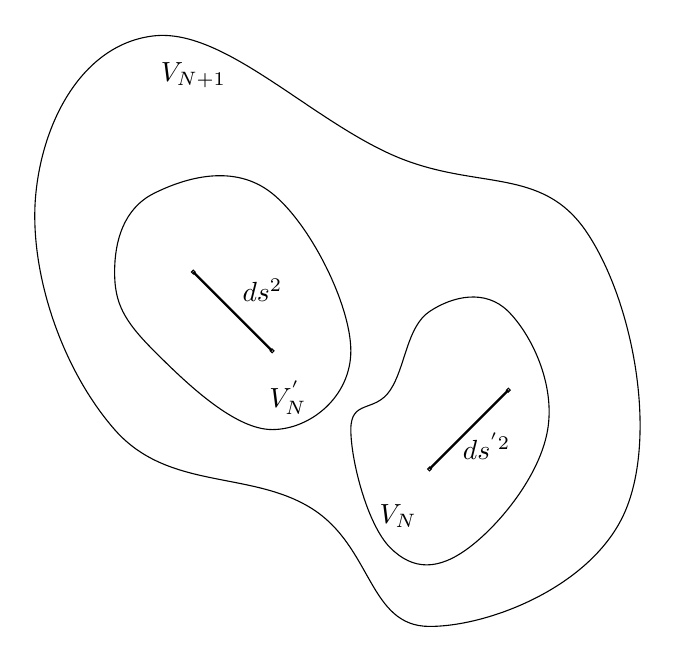
\begin{tikzpicture}
\draw  plot[smooth cycle, tension=.7] coordinates {(-3.5,6.5) (-0.5,5) (2,4) (2.5,0.5) (0,-1) (-1.5,0.5) (-4,1.5) (-5,4.5)};
\draw  plot[smooth cycle, tension=.7] coordinates {(-3.5,4.5) (-2,4.5) (-1,2.5) (-2,1.5) (-3.5,2.5) (-4,3.5)};
\draw  plot[smooth cycle, tension=.7] coordinates {(1,3) (1.5,1.5) (0.5,0) (-0.5,0) (-1,1.5) (-0.5,2) (0,3)};
\node at (-3,6) {$V_{N+1}$};
\node at (-1.8,1.9) {$V^{'}_{N}$};
\node at (-0.4,0.4) {$V_{N}$};
\coordinate (v1) at (-3,3.5) {};
\coordinate (v2) at (-2,2.5) {};
\draw[fill=white](v1) circle(0.7pt)node[{anchor=north }] {};
\draw[fill=white](v2) circle(0.7pt)node[{anchor=north }] {};
\draw[thick]   (v1) -- (v2);
\coordinate (v3) at (1,2) {};
\coordinate (v4) at (0,1) {};
\draw[fill=white](v3) circle(0.7pt)node[{anchor=north }] {};
\draw[fill=white](v4) circle(0.7pt)node[{anchor=north }] {};
\draw[thick]  (v3) -- (v4);
\node at (-2.5,3)[anchor = south west] {$ds^2$};
\node [anchor = south west] at (0.3,1) {$ds^{'2}$};
\end{tikzpicture}\\
\end{minipage}\hfill
\caption{Embedded $V_N$ spaces}
\label{fig:p109_Ex5_a}
\end{figure}
\begin{align*}
 ds^{'2} &= ds^2\\
 \Rightarrow \spatie a^{'}_{mn} dx^{'m}dx^{'n} &= a_{mn}dx^{m} dx^{n}\\
 \Rightarrow \spatie k a_{mn} dx^{'m}dx^{'n} &= a_{mn}dx^{m} dx^{n}\\
 \Rightarrow \spatie dx^{'m} &= \frac{1}{\sqrt{k}}dx^{m}
\end{align*}
We have also
\begin{align*}
 a^{'}_{mk}a^{'kn} &= \delta^n_m\\
 \Rightarrow \spatie ka_{mp}a^{'pn} &= \delta^n_m\\
 \Rightarrow \spatie a^{'pn} &= \frac{1}{k}a^{pn}
\end{align*}
And get the following relations
\begin{align*}
\left \{ \begin{array}{l}
 [mn,r]^{'} = \sqrt{k}^3[mn,r]\\\\
 \Gamma^{'r}_{.mn} =\sqrt{k}\Gamma^{r}_{.mn}
 \end {array}\right.
 \end{align*}
 \begin{align*}
 \Rightarrow \spatie &R^{'s}_{\ .rmn} = \frac{\partial \Gamma^{'s}_{\ .rn}}{\partial x^{'m}} + \dots\\
 \Rightarrow \spatie &R^{'s}_{\ .rmn} = \frac{\sqrt{k}\partial \Gamma^{s}_{.rn}}{\partial \left(\frac{x^{m}}{\sqrt{k}}\right)} + \dots\\
 \Rightarrow \spatie &R^{'s}_{\ .rmn} = k R^{s}_{.rmn}\\
 \times \ a^{'ks}\spatie \Rightarrow \spatie & a^{'ks}R^{'s}_{\ .rmn} = k a^{'ks}R^{s}_{.rmn}\\
 \Rightarrow \spatie &R^{'}_{krmn} = k \frac{1}{k}a^{ks}R^{s}_{.rmn}\\
 \Rightarrow \spatie & R^{'}_{krmn} =R_{krmn}\\
 R_{rm} = R^n_{.rmn} \quad \Rightarrow \spatie &R^{'}_{\ mn} = k R_{rmn}\\
 R = a^{mn}R_{mn} \quad \Rightarrow \spatie &R^{'} = a^{'mn}R^{'}_{mn}\\
 \Rightarrow \spatie  &R^{'} = \frac{1}{k}a^{mn}k R_{mn}\\
 \Rightarrow \spatie  &R^{'} =  R
\end{align*}\\\\
$\mathbf{Summary}$\\
 \begin{align*}
R^{'s}_{\ .rmn} &= k R^{s}_{.rmn}\\
R^{'}_{krmn} &=R_{krmn}\\
R^{'}_{ mn} &= k R_{rmn}\\
R^{'} &=  R
\end{align*}
$$\blacklozenge$$
\newpage





\section{p109 - Exercise 6}
\begin{tcolorbox}
For an orthogonal coordinates system in a $V_2$ we have $$ ds^2=a_{11}\left( dx^1\right)^2+a_{22}\left( dx^2\right)^2$$
Show that 
$$\frac{1}{a}R_{1212}= -\half\frac{1}{\sqrt{a}}\left[\partial_1\left(\frac{1}{\sqrt{a}}\partial_1 a_{22}\right)+\partial_2\left(\frac{1}{\sqrt{a}}\partial_2 a_{11}\right)\right]$$
\end{tcolorbox}
We have 
\begin{align}
\left(a_{mn}\right)= \begin{pmatrix}
 a_{11}& 0 \\
 0& a_{22} \\
\end{pmatrix}\quad \left(a^{mn}\right)= \frac{1}{a}\begin{pmatrix}
 a_{22}& 0 \\
 0& a_{11} \\
\end{pmatrix}\quad
 a= a_{11}a_{22}
\end{align}
We have also \\
\begin{align}
R &= -\frac{2}{a}R_{1212}\\
R =  a^{mn}R_{mn}\quad\Rightarrow\quad R &= a^{11}R_{11}+ a^{22}R_{22}
\end{align}
Looking at the pattern generated by equations $(2)$ and $(3)$ suggests that using these equations could lead to the proposed equation. Let's have a try ...
\begin{align}
& \left \{ \begin{array}{ll}
\Gamma^1_{11} = \half\frac{a_{22}}{a}\partial_1 a_{11}&\Gamma^1_{22} =- \half\frac{a_{22}}{a}\partial_1 a_{22}\\\\
\Gamma^2_{11} =- \half\frac{a_{11}}{a}\partial_2 a_{11}&\Gamma^2_{22} = \half\frac{a_{11}}{a}\partial_2 a_{22}\\\\
\Gamma^1_{12} = \half\frac{a_{22}}{a}\partial_2 a_{11}&\Gamma^2_{12} = \half\frac{a_{11}}{a}\partial_1 a_{22}
\end {array}\right. \\
\text{3.205.}\quad\Rightarrow\quad & R_{rm} = \half\partial_{rm} \log a - \half \Gamma^p_{rm}\partial_p \log a-\partial_n\Gamma^n_{rm} + \Gamma^p_{rn}\Gamma^n_{pm}\\
\Rightarrow\quad &\left \{ \begin{array}{l}
 R_{11} =  \half\partial_{11} \log a - \half \Gamma^1_{11}\partial_1 \log a- \half \Gamma^2_{11}\partial_2 \log a \\
 -\partial_1\Gamma^1_{11}-\partial_2\Gamma^2_{11} + 
 \\ \Gamma^1_{11}\Gamma^1_{11}+ \Gamma^1_{12}\Gamma^2_{11}+ \Gamma^2_{11}\Gamma^1_{21}+ \Gamma^2_{12}\Gamma^2_{21}\\\\
  R_{22} =  \half\partial_{22} \log a - \half \Gamma^1_{22}\partial_1 \log a- \half \Gamma^2_{22}\partial_2 \log a \\
 -\partial_1\Gamma^1_{22}-\partial_2\Gamma^2_{22} + 
 \\ \Gamma^1_{21}\Gamma^1_{12}+ \Gamma^1_{22}\Gamma^2_{12}+ \Gamma^2_{21}\Gamma^1_{22}+ \Gamma^2_{22}\Gamma^2_{22}\\\\
 \end {array}\right.
 \end{align}
 %**************************************************
 \begin{align}
 \Rightarrow\quad &\left \{ \begin{array}{l}
 R_{11} =  \half\partial_{11} \log a - \half \half\frac{a_{22}}{a}\partial_1 a_{11}\partial_1 \log a- \half (- \half\frac{a_{11}}{a}\partial_2 a_{11})\partial_2 \log a \\
 -\partial_1(\half\frac{a_{22}}{a}\partial_1 a_{11})-\partial_2(- \half\frac{a_{11}}{a}\partial_2 a_{11}) + 
 \\ \half\frac{a_{22}}{a}\partial_1 a_{11}\half\frac{a_{22}}{a}\partial_1 a_{11}+ \half\frac{a_{22}}{a}\partial_2 a_{11}(- \half\frac{a_{11}}{a}\partial_2 a_{11})+ \\
 (- \half\frac{a_{11}}{a}\partial_2 a_{11})\half\frac{a_{22}}{a}\partial_2 a_{11}+ \half\frac{a_{11}}{a}\partial_1 a_{22}\half\frac{a_{11}}{a}\partial_1 a_{22}\\\\
  R_{22} =  \half\partial_{22} \log a - \half (- \half\frac{a_{22}}{a}\partial_1 a_{22})\partial_1 \log a- \half \half\frac{a_{11}}{a}\partial_2 a_{22}\partial_2 \log a \\
 -\partial_1(- \half\frac{a_{22}}{a}\partial_1 a_{22})-\partial_2(\half\frac{a_{11}}{a}\partial_2 a_{22}) + 
 \\ \half\frac{a_{22}}{a}\partial_2 a_{11}\half\frac{a_{22}}{a}\partial_2 a_{11}+ (- \half\frac{a_{22}}{a}\partial_1 a_{22})\half\frac{a_{11}}{a}\partial_1 a_{22}+ \\
 \half\frac{a_{11}}{a}\partial_1 a_{22}(- \half\frac{a_{22}}{a}\partial_1 a_{22})+ \half\frac{a_{11}}{a}\partial_2 a_{22}\half\frac{a_{11}}{a}\partial_2 a_{22}\\\\
 \end {array}\right.
 \end{align}
 Simplifying the notational burden by  replacing $a_{11}$ by $\gamma$ and $a_{22}$ by $\eta$:
  \begin{align}
 \Rightarrow\quad &\left \{ \begin{array}{l}
 R_{11} =  \half\partial_{11} \log a - \half \half\frac{1}{\gamma}\partial_1 \gamma\partial_1 \log a+ \half \half\frac{1}{\eta}\partial_2 \gamma\partial_2 \log a \\
 -\half\partial_1(\frac{1}{\gamma}\partial_1 \gamma)+\half\partial_2(\frac{1}{\eta}\partial_2 \gamma)
 \\ + \half\half\frac{1}{\gamma}\frac{1}{\gamma}\partial_1 \gamma\partial_1 \gamma- \half\half\frac{1}{\gamma}\frac{1}{\eta}\partial_2 \gamma \partial_2 \gamma \\
 - \half\half\frac{1}{\gamma}\frac{1}{\eta}\partial_2 \gamma\partial_2 \gamma+ \half\half\frac{1}{\eta}\frac{1}{\eta}\partial_1 \eta\partial_1 \eta\\\\
  R_{22} =  \half\partial_{22} \log a + \half\half\frac{1}{\gamma}\partial_1 \eta\partial_1 \log a- \half \half\frac{1}{\eta}\partial_2 \eta\partial_2 \log a \\
 +\half\partial_1(\frac{1}{\gamma}\partial_1 \eta)-\half\partial_2(\frac{1}{\eta}\partial_2 \eta)  
 \\ + \half\half\frac{1}{\gamma}\frac{1}{\gamma}\partial_2 \gamma\partial_2 \gamma- \half\half\frac{1}{\gamma}\frac{1}{\eta}\partial_1 \eta\partial_1 \eta \\
 - \half\half\frac{1}{\gamma}\frac{1}{\eta}\partial_1 \eta \partial_1 \eta+ \half\half\frac{1}{\eta}\frac{1}{\eta}\partial_2 \eta\partial_2 \eta\\\\
 \end {array}\right.
 \end{align}
 %****************************************************
 Noting that $\partial_{ii}\log a = \partial_{i}\left(\frac{1}{a_{11}}\partial_{i} a_{11}\right) + \partial_{i}\left(\frac{1}{a_{22}}\partial_{i} a_{22}\right)$ and $\partial_{i}\log a = \frac{1}{a_{11}}\partial_{i} a_{11} + \frac{1}{a_{22}}\partial_{i} a_{22}\quad (i=1,2)$, we get:\\
 \begin{align}
 %****************************
  \left| \begin{array}{c}
 2R_{11} = \\\\
  \underbrace{\partial_{1}\left(\frac{1}{\gamma}\partial_{1} \gamma\right)}_{*}+\partial_{1}\left(\frac{1}{\eta}\partial_{1} \eta\right) \\\\
  - \underbrace{\half \frac{1}{\gamma}\frac{1}{\gamma}(\partial_1 \gamma )^2}_{-} - \half \frac{1}{\gamma}\frac{1}{\eta}\partial_1 \gamma \partial_{1} \eta \\\\
   + \half\frac{1}{\gamma}\frac{1}{\eta}(\partial_2 \gamma)^2 +\half\frac{1}{\eta}\frac{1}{\eta}\partial_2 \gamma \partial_{2} \eta \\\\
 -\underbrace{\partial_1(\frac{1}{\gamma}\partial_1 \gamma)}_{*}+\partial_2( \frac{1}{\eta}\partial_2 \gamma)  
 \\\\
  + \underbrace{\half\frac{1}{\gamma}\frac{1}{\gamma}(\partial_1 \gamma)^2}_{-}- \underbrace{\half \frac{1}{\gamma}\frac{1}{\eta}(\partial_2 \gamma )^2}_{+} \\\\
 - \underbrace{\half \frac{1}{\gamma}\frac{1}{\eta}(\partial_2 \gamma)^2}_{+}+ \half\frac{1}{\eta}\frac{1}{\eta}(\partial_1 \eta)^2\\\\
 \end {array}\quad
 \right.
 \left | \begin{array}{c}
  2R_{22} = \\\\
    \partial_{2}\left(\frac{1}{\gamma}\partial_{2} \gamma\right)+\underbrace{\partial_{2}\left(\frac{1}{\eta}\partial_{2} \eta\right)}_{*} \\\\
   + \half\frac{1}{\gamma}\frac{1}{\gamma}\partial_{1} \gamma\partial_1 \eta  + \half\frac{1}{\gamma}\frac{1}{\eta}(\partial_1 \eta )^2 \\\\
   - \half \frac{1}{\gamma}\frac{1}{\eta}\partial_{2} \gamma\partial_2 \eta  - \underbrace{\half \frac{1}{\eta}\frac{1}{\eta}(\partial_2 \eta)^2 }_{-} \\\\
 +\partial_1(\frac{1}{\gamma}\partial_1 \eta)-\underbrace{\partial_2( \frac{1}{\eta}\partial_2 \eta)}_{*}  
 \\\\
  + \half\frac{1}{\gamma}\frac{1}{\gamma}(\partial_2 \gamma)^2- \underbrace{\half\frac{1}{\gamma}\frac{1}{\eta}(\partial_1 \eta )^2}_{+}\\\\
 - \underbrace{\half\frac{1}{\gamma}\frac{1}{\eta}(\partial_1 \eta)^2}_{+}+ \underbrace{\half \frac{1}{\eta}\frac{1}{\eta}(\partial_2 \eta)^2}_{-}\\\\
 \end {array}\right|
\end{align}
 \begin{align}
 %****************************
  \Rightarrow\quad &\left| \begin{array}{c}
  2R_{11} = \\\\
 \partial_{1}\left(\frac{1}{\eta}\partial_{1} \eta\right)+ \partial_2( \frac{1}{\eta}\partial_2 \gamma)\\\\
  + \half\frac{1}{\eta}\frac{1}{\eta}(\partial_1 \eta)^2 - \half\frac{1}{\gamma}\frac{1}{\eta}(\partial_2 \gamma)^2\\\\ - \half \frac{1}{\gamma}\frac{1}{\eta}\partial_1 \gamma \partial_{1} \eta  +\half\frac{1}{\eta}\frac{1}{\eta}\partial_2 \gamma \partial_{2} \eta \\
\end{array}\right.\quad
\left|\begin{array}{c}
  \spatie 2R_{22} = \\\\
    \partial_1(\frac{1}{\gamma}\partial_1 \eta) +\partial_{2}\left(\frac{1}{\gamma}\partial_{2} \gamma\right)\\\\
    - \half\frac{1}{\gamma}\frac{1}{\eta}(\partial_1 \eta )^2 + \half\frac{1}{\gamma}\frac{1}{\gamma}(\partial_2 \gamma)^2\\\\
  + \half\frac{1}{\gamma}\frac{1}{\gamma}\partial_{1} \gamma\partial_1 \eta  - \half \frac{1}{\gamma}\frac{1}{\eta}\partial_{2} \gamma\partial_2 \eta  \\
 \end {array}\right|
 \end{align}\\\\ 
  %****************************
  
  Be $R = \frac{1}{\gamma}R_{11}+ \frac{1}{\eta}R_{22}$, all first order derivatives vanish and we get,\\\\
  \begin{align}
  \frac{1}{\gamma}R_{11}+ \frac{1}{\eta}R_{22} = & 
 \half \left[ \frac{1}{\eta}\partial_1(\frac{1}{\gamma}\partial_1 \eta)+ \frac{1}{\gamma} \partial_{1}(\frac{1}{\eta}\partial_{1} \eta)\right]
    + \half  \left[\frac{1}{\gamma}\partial_{2}(\frac{1}{\gamma}\partial_{2} \gamma)+ \frac{1}{\eta}\partial_2( \frac{1}{\eta}\partial_2 \gamma) \right] 
\end{align}\\
We further simplify this expression. Considering the symmetry of $(11)$ we only explicit the calculations for the first terms in $\partial_1$.
\begin{align}
 \frac{1}{\eta}\partial_1(\frac{1}{\gamma}\partial_1 \eta)+ \frac{1}{\gamma} \partial_{1}(\frac{1}{\eta}\partial_{1} \eta)&=\frac{1}{\eta}\partial_1(\frac{1}{\sqrt{\gamma}}\frac{1}{\sqrt{\gamma}}\frac{\sqrt{\eta}}{\sqrt{\eta}}\partial_1 \eta)+ \frac{1}{\gamma} \partial_{1}(\frac{1}{\sqrt{\eta}}\frac{1}{\sqrt{\eta}}\frac{\sqrt{\gamma}}{\sqrt{\gamma}}\partial_{1} \eta)\\
 &=\frac{1}{\eta}\partial_1\left[\left(\frac{\eta}{\gamma}\right)^{\half}\frac{1}{\sqrt{a}}\partial_1 \eta\right]+ \frac{1}{\gamma} \partial_{1}\left[\left(\frac{\eta}{\gamma}\right)^{-\half}\frac{1}{\sqrt{a}}\partial_{1} \eta\right]\\
 &=\left \{ \begin{array}{l}
\underbrace{\frac{1}{\eta}\left(\frac{\eta}{\gamma}\right)^{\half}}_{= \frac{1}{\sqrt{a}}}\partial_1\left[\frac{1}{\sqrt{a}}\partial_1 \eta\right]+ \underbrace{\frac{1}{\gamma} \left(\frac{\eta}{\gamma}\right)^{-\half}}_{= \frac{1}{\sqrt{a}}}\partial_{1}\left[\frac{1}{\sqrt{a}}\partial_{1} \eta\right]\\\\
+\frac{1}{\sqrt{a}}\partial_1 \eta\underbrace{\left[\frac{1}{\eta}\partial_1\left(\frac{\eta}{\gamma}\right)^{\half}+ \frac{1}{\gamma} \partial_{1}\left(\frac{\eta}{\gamma}\right)^{-\half}\right]}_{=0}
 \end {array}\right.\\
  &= 2\frac{1}{\sqrt{a}}\partial_1\left[\frac{1}{\sqrt{a}}\partial_1 a_{22}\right]\\
  \Rightarrow \quad  \half \left[ \frac{1}{\eta}\partial_1(\frac{1}{\gamma}\partial_1 \eta) + \frac{1}{\gamma} \partial_{1}(\frac{1}{\eta}\partial_{1} \eta)\right] &=  \frac{1}{\sqrt{a}}\partial_1\left[\frac{1}{\sqrt{a}}\partial_1 a_{22}\right]  
\end{align}
Using $(16)$ and the same calculations for the terms in $\partial_2$ and using $(2)$ and $(3)$ we  get $$\frac{1}{a}R_{1212}= -\half\frac{1}{\sqrt{a}}\left[\partial_1\left(\frac{1}{\sqrt{a}}\partial_1 a_{22}\right)+\partial_2\left(\frac{1}{\sqrt{a}}\partial_2 a_{11}\right)\right]$$
$$\blacklozenge$$
\newpage

\section{p109 - Exercise 7}
\begin{tcolorbox}
Suppose that in a $V_3$ the metric is :$$ ds^2= (h_1dx^1)^2+(h_2dx^2)^2+(h_3dx^3)^2$$ where $h_1, h_2, h_3$ are functions of the three coordinates. Calculate the curvature  tensor in terms of the $h^{'}s$ and their derivatives. Check your result by nothing that the curvature tensor will vanish if $h_1$ is a function of $x^1$ only, $h_2$ a function of $x^2$ only, and $h_3$  a function of $x^3$ only.
\end{tcolorbox}
From $\mathbf{3.115.}$ and $\mathbf{3.115.}$ we get for the non vanishing components of the covariant curvature tensor($6$ independent components to calculate):
\begin{align*}
R_{1212} =\left\{ \begin{array}{c}
- R_{1221} \\
- R_{2112} \\
 R_{2121} \\
\end{array}\right.  \quad R_{2323} =\left\{ \begin{array}{c}
- R_{2332} \\
- R_{3223} \\
 R_{3232} \\
\end{array}\right.  \quad R_{1313} =\left\{ \begin{array}{c}
- R_{1331} \\
- R_{3113} \\
 R_{3131} \\
\end{array}\right.  \\
R_{1213} =\left\{ \begin{array}{c}
- R_{1231} \\
 R_{1312} \\
 -R_{1321} \\
- R_{2113} \\
 R_{2131} \\
 -R_{3112} \\
 R_{3121} \\
\end{array}\right.  \quad
R_{1223} =\left\{ \begin{array}{c}
- R_{1232} \\
- R_{2123} \\
 R_{2132} \\
 R_{2312} \\
 -R_{2321} \\
 R_{3212} \\
 -R_{3221} \\
\end{array}\right. \quad
R_{1323} =\left\{ \begin{array}{c}
- R_{1332} \\
 R_{2313} \\
 -R_{2331} \\
- R_{3123} \\
 R_{3132} \\
 -R_{3213} \\
 R_{3231} \\
\end{array}\right.
\end{align*}
The metric tensors:
\begin{align*}
(a_{mn})  = \begin{pmatrix}
 h^2_1& 0&0 \\
 0& h^2_2&0 \\
 0& 0&h^2_3
\end{pmatrix}\quad (a^{mn})  = \begin{pmatrix}
 \frac{1}{h^2_1}& 0&0 \\
 0& \frac{1}{h^2_2}&0 \\
 0& 0&\frac{1}{h^2_3}
\end{pmatrix}
\end{align*}
The Christoffel symbols:
\begin{align*}
\begin{array}{lll}
\ [11,1]= h_{1} \partial_{1} h_{1} & [11,2]=- h_{1} \partial_{2} h_{1} & [11,3]= -h_{1} \partial_{3} h_{1}\\
\ [12,1]= h_{1} \partial_{2} h_{1} & [12,2]= h_{2} \partial_{1} h_{2} & [12,3]= 0\\
\ [22,1]= -h_{2} \partial_{1} h_{2} & [22,2]=h_{2} \partial_{2} h_{2} & [22,3]= -h_{2} \partial_{3} h_{2}\\
\  [23,1]= 0 & [23,2]= h_{2} \partial_{3} h_{2} & [23,3]= h_{3} \partial_{2} h_{3}\\
\ [33,1]= -h_{3} \partial_{1} h_{3} & [33,2]=- h_{3} \partial_{2} h_{3} & [33,3]= -h_{3} \partial_{3} h_{3}\\
\ [31,1]= h_{1} \partial_{3} h_{1} & [31,2]=0 & [31,3]= h_{3} \partial_{1} h_{3}\\
\end{array}
\end{align*}
\begin{align*}
\begin{array}{lll}
\Gamma^1_{11}=\frac{1}{h_{1}}\partial_{1}{h_{1}} &\Gamma^2_{11}=-\frac{h_{1}}{h_{2}^2}\partial_{2}{h_{1}}  & \Gamma^3_{11}= -\frac{h_{1}}{h_{3}^2}\partial_{3}{h_{1}}   \\
\Gamma^1_{12}= \frac{1}{h_{1}}\partial_{2}{h_{1}} &\Gamma^2_{12}=\frac{1}{h_{2}}\partial_{1}{h_{2}} & \Gamma^3_{12}=0\\
\Gamma^1_{22}= -\frac{h_{2}}{h_{1}^2}\partial_{1}{h_{2}} &\Gamma^2_{22}=\frac{1}{h_{2}}\partial_{2}{h_{2}} & \Gamma^3_{22}=-\frac{h_{2}}{h_{3}^2}\partial_{3}{h_{2}} \\
\Gamma^1_{23}=0 &\Gamma^2_{23}=\frac{1}{h_{2}}\partial_{3}{h_{2}} & \Gamma^3_{23}= \frac{1}{h_{3}}\partial_{2}{h_{3}}\\
\Gamma^1_{33}= -\frac{h_{3}}{h_{1}^2}\partial_{1}{h_{3}}&\Gamma^2_{33}=-\frac{h_{3}}{h_{2}^2}\partial_{2}{h_{3}} & \Gamma^3_{33}= \frac{1}{h_{3}}\partial_{3}{h_{3}}\\
\Gamma^1_{31}=\frac{1}{h_{1}}\partial_{3}{h_{1}} &\Gamma^2_{31}=0 & \Gamma^3_{31}=\frac{1}{h_{3}}\partial_{1}{h_{3}} \\
\end{array}
\end{align*}
We use $3.113.$ $$R_{rsmn}= \partial_m[sn,r] -\partial_n[sm,r]+\Gamma^p_{sm}[rn,p]-\Gamma^p_{sn}[rm,p]$$\\

Note that we only have to perform the full calculation for two curvature tensors e.g. $R_{1212}$ and $R_{1213}$  as the others can be retrieved by using adequate indices renaming and use of the identities $3.115.$
\begin{align*}
R_{1212}&=
-h_2\partial_{11}^2(h_2)-h_1\partial_{22}^2(h_1)
+\frac{h_2}{h_1}\partial_1 h_1\partial_1 h_2+\frac{h_1}{h_2}\partial_2 h_1\partial_2 h_2-\frac{h_1 h_2}{h_3^2}\partial_3 h_1\partial_3 h_2\\
R_{2323}&=
-h_3\partial_{22}^2(h_3)-h_2\partial_{33}^2(h_2)
+\frac{h_3}{h_2}\partial_2 h_2\partial_2 h_3+\frac{h_2}{h_3}\partial_3 h_2\partial_3 h_3-\frac{h_2 h_3}{h_1^2}\partial_1 h_2\partial_1 h_3\\
R_{1313}&=
-h_3\partial_{11}^2(h_3)-h_1\partial_{33}^2(h_1)
+\frac{h_3}{h_1}\partial_1 h_1\partial_1 h_3+\frac{h_1}{h_3}\partial_3 h_1\partial_3 h_3-\frac{h_1 h_3}{h_2^2}\partial_2 h_1\partial_2 h_3
\end{align*}
\begin{align*}
R_{1213}&=-h_1\partial_{32}^2(h_1)+\frac{h_1}{h_3}\partial_2 h_3\partial_3 h_1+\frac{h_1}{h_2}\partial_2 h_1\partial_3 h_2\\
R_{1223}&=h_2\partial_{31}^2(h_2)-\frac{h_2}{h_1}\partial_1 h_2\partial_3 h_1-\frac{h_2}{h_3}\partial_3 h_2\partial_1 h_3\\
R_{1323}&=
-h_3\partial_{21}^2(h_3)+\frac{h_3}{h_1}\partial_1 h_3\partial_3 h_1+\frac{h_3}{h_2}\partial_2 h_3\partial_1 h_2
\end{align*}
And, indeed, all curvature tensors vanish when the $h_i$ are only a function of the indices' dimension.
$$\blacklozenge$$
\newpage


\section{p109 - Exercise 8}
\begin{tcolorbox}
In relativity we encounter the metric form $$ \Phi= e^{\alpha} + e^{x^1}\left[ \left( dx^2 \right)^2 + \sin^2 x^2 \left(dx^3 \right)^2 \right] - e^{\gamma}\left(dx^4\right)^2$$ where $\alpha$ and $\gamma$ are functions of $x^1$ and $x^4$ only.\\
Show that the complete set of non-zero components of the Einstein tensor (see equation (3.214)) for the form given above are as follows
\begin{align*}
G^1_{.1} &= e^{-\alpha}\left( -\kwart -\half\gamma_1\right) + e^{-x^1}\\
G^2_{.2} &= e^{\alpha} \left(-\kwart - \half \gamma_{11} - \kwart \gamma_1^2 -\kwart\gamma_1+\kwart \alpha _1 +\kwart \alpha _1 \gamma_1 \right) \\
&+e^{\gamma} \left(\half \alpha_{44} + \kwart\alpha_4^2 -\kwart\alpha_4\gamma_4\right)\\
G^3_{.3} &= G^2_{.2} \\
G^4_{.4} &= e^{-\alpha}\left( -\frac{3}{4} -\half\alpha_1\right) + e^{-x^1}\\
 e^{\alpha} G^4_{.1} &= -e^{\gamma} G^4_{.1} = -\half \alpha_4
\end{align*}
The subscript on $\alpha$ and $\gamma$ indicate partial derivatives with respect to $x^1$ and $x^4$.
\end{tcolorbox}
We have 
\begin{align}
\left(a_{mn}\right)= \begin{pmatrix}
 e^{\alpha}& 0&0&0 \\
 0& e^{x^1} &0&0\\
 0& 0 &e^{x^1}\sin^2 x^2&0\\
 0& 0 &0&-e^{\gamma}\\
\end{pmatrix}\quad 
\left(a^{mn}\right)= \begin{pmatrix}
 {e^{-\alpha}}& 0&0&0 \\
 0& {e^{-x^1}} &0&0\\
 0& 0 &\frac{e^{-x^1}}{\sin^2 x^2}&0\\
 0& 0 &0&-{e^{-\gamma}}\\
\end{pmatrix}
\end{align}
And will use the following definitions:
\begin{align}
 G^n_{.t} &= R^n_{.t} - \half \delta^n_t R\\
 R^n_{.t} &= a^{nk}R_{kt}\\
 R_{kt} &= a^{sn}R_{sktn}\\
 R &= a^{kt}R_{kt}
\end{align}
Considering that the non-diagonal components of $a_{mn}$ vanish and as $R_{sktn}=0$ when $s=k$ or $t=n$, we can write :
\begin{align}
\begin{pmatrix}
 R_{11}\\
 R_{22}\\
 R_{33}\\
 R_{44}\\
\end{pmatrix}&=
\begin{pmatrix}
 0& R_{2112} & R_{3113} & R_{4114} \\
 R_{1221}& 0 &  R_{3223}& R_{4224} \\
 R_{1331}&R_{2332}  & 0 & R_{4334} \\
 R_{1441}& R_{2442} & R_{3443}& 0 \\
\end{pmatrix}\begin{pmatrix}
 a^{11}\\
 a^{22}\\
 a^{33}\\
 a^{44}\\
\end{pmatrix}
\end{align}
\begin{align}
\begin{pmatrix}
 R_{12}\\
 R_{13}\\
 R_{14}\\
 R_{23}\\
 R_{24}\\
 R_{34}\\
\end{pmatrix}&=
\begin{pmatrix}
 0& 0& R_{3123} & R_{4124}  \\
 0& R_{2132} &  0& R_{4134} \\
 0&R_{2142}  &R_{3143} & 0 \\
 R_{1231}& 0 &0& R_{4234} \\
 R_{1241}& 0 &R_{3243}& 0 \\
 R_{1341}& R_{2342} &0& 0 \\
\end{pmatrix}\begin{pmatrix}
 a^{11}\\
 a^{22}\\
 a^{33}\\
 a^{44}\\
\end{pmatrix}\\
\end{align}
The Christoffel symbols of the first kind are:
\begin{align}
\begin{array}{llll}
 \ [11,1]=\half\alpha _1 e^{\alpha}& \ [11,2]=0& \ [11,3]= 0& \ [11,4]=-\half\alpha _4 e^{\alpha} \\
 \ [12,1]=0& \ [12,2]=\half e^{x^1}& \ [12,3]= 0& \ [12,4]=0 \\
 \ [13,1]=0& \ [13,2]=0& \ [13,3]= \half e^{x^1}\sin^2 x^2& \ [13,4]=0\\
 \ [14,1]=\half\alpha _4 e^{\alpha}& \ [14,2]=0& \ [14,3]= 0& \ [14,4]=-\half\gamma _1 e^{\gamma} \\
 \ [22,1]=-\half e^{x^1}& \ [22,2]=0& \ [22,3]= 0& \ [22,4]=0\\
 \ [23,1]=0& \ [23,2]=0& \ [23,3]= \half e^{x^1}\sin 2x^2  & \ [23,4]=0\\
 \ [24,1]=0& \ [24,2]=0& \ [24,3]= 0& \ [24,4]=0 \\
 \ [33,1]=-\half e^{x^1}sin^2 x^2& \ [33,2]=-\half e^{x^1}\sin 2x^2 & \ [33,3]= 0& \ [33,4]=0\\
 \ [34,1]=0& \ [34,2]=0& \ [34,3]= 0& \ [34,4]=0 \\
 \ [44,1]=\half \gamma _1 e^{\gamma}& \ [44,2]=0& \ [44,3]= 0& \ [44,4]=-\half\gamma _4 e^{\gamma} \\
\end{array}
\end{align}
We use $3.114.$ and considering that $a_{mn}= a^{mn}= 0$ for $m\ne n$: $$R_{rsmn}= \left\{\begin{array}{l}
\half\left(\partial^2_{sm}a_{rn}+\partial^2_{rn}a_{sm}\right)\\
+ \frac{1}{e^{\alpha}}\left( [rn,1] [sm,1] -[rm,1] [sn,1]  \right)\\
+ \frac{1}{e^{x^1}}\left([rn,2] [sm,2] -[rm,2][sn,2] \right)\\
+ \frac{1}{e^{x^1}\sin^2 x^2}\left( [rn,3][sm,3]-[rm,3][sn,3]  \right)\\
-\frac{1}{e^{\gamma}}\left( [rn,4][sm,4] -[rm,4][sn,4]  \right)
\end{array}\right.$$\\


%************************************************************
Giving:
\begin{align}
R_{2112}&= \left\{\begin{array}{l}
\half\left(\partial^2_{11} a_{22}+\partial^2_{22} a_{11}\right)\\\\
+ \frac{1}{e^{\alpha}}\left( [22,1] [11,1] -[21,1] [12,1]  \right)\\\\
+ \frac{1}{e^{x^1}}\left( [22,2]  [11,2] -[21,2] [12,2]  \right)\\\\
+ \frac{1}{e^{x^1}\sin^2 x^2}\left( [22,3] [11,3] -[21,3] [12,3]   \right)\\\\
-\frac{1}{e^{\gamma}}\left( [22,4]  [11,4] -[21,4] [12,4]   \right)
\end {array}\right.\\
\end{align}
\begin{align}
R_{3113}&= \left\{\begin{array}{l}
\half\left(\partial^2_{11} a_{33}+\partial^2_{33} a_{11}\right)\\\\
+ \frac{1}{e^{\alpha}}\left( [33,1] [11,1] -[31,1] [13,1]  \right)\\\\
+ \frac{1}{e^{x^1}}\left( [33,2] [11,2] -[31,2] [13,2]   \right)\\\\
+ \frac{1}{e^{x^1}\sin^2 x^2}\left( [33,3] [11,3] -[31,3] [13,3]  \right)\\\\
-\frac{1}{e^{\gamma}}\left( [33,4]  [11,4] -[31,4] [13,4]   \right)
\end {array}\right.\\
\end{align}
\begin{align}
R_{4114}&= \left\{\begin{array}{l}
\half\left(\partial^2_{11} a_{44}+\partial^2_{44} a_{11}\right)\\\\
+ \frac{1}{e^{\alpha}}\left( [44,1] [11,1] -[41,1] [14,1]  \right)\\\\
+ \frac{1}{e^{x^1}}\left( [44,2]  [11,2]  -[41,2] [14,2]  \right)\\\\
+ \frac{1}{e^{x^1}\sin^2 x^2}\left( [44,3]  [11,3] -[41,3] [14,3]  \right)\\\\
-\frac{1}{e^{\gamma}}\left( [44,4] [11,4] -[41,4] [14,4]  \right)
\end {array}\right.\\
\end{align}
\begin{align}
R_{3223}&= \left\{\begin{array}{l}
\half\left(\partial^2_{22} a_{33}+\partial^2_{33} a_{22}\right)\\\\
+ \frac{1}{e^{\alpha}}\left( [33,1] [22,1] -[32,1] [23,1]  \right)\\\\
+ \frac{1}{e^{x^1}}\left( [33,2] [22,2] -[32,2] [23,2]   \right)\\\\
+ \frac{1}{e^{x^1}\sin^2 x^2}\left( [33,3]  [22,3] -[32,3] [23,3]  \right)\\\\
-\frac{1}{e^{\gamma}}\left( [33,4]  [22,4] -[32,4] [23,4]   \right)
\end {array}\right.\\
\end{align}
\begin{align}
R_{4224}&= \left\{\begin{array}{l}
\half\left(\partial^2_{22} a_{44}+\partial^2_{44} a_{22}\right)\\\\
+ \frac{1}{e^{\alpha}}\left( [44,1] [22,1] -[42,1] [24,1]  \right)\\\\
+ \frac{1}{e^{x^1}}\left( [44,2] [22,2] -[42,2] [24,2]  \right)\\\\
+ \frac{1}{e^{x^1}\sin^2 x^2}\left( [44,3] [22,3] -[42,3] [24,3]  \right)\\\\
-\frac{1}{e^{\gamma}}\left( [44,4] [22,4] -[42,4] [24,4]  \right)
\end {array}\right.\\
\end{align}
\begin{align}
R_{4334}&= \left\{\begin{array}{l}
\half\left(\partial^2_{33} a_{44}+\partial^2_{44} a_{33}\right)\\\\
+ \frac{1}{e^{\alpha}}\left( [44,1] [33,1] -[43,1] [34,1]  \right)\\\\
+ \frac{1}{e^{x^1}}\left( [44,2] [33,2] -[43,2] [34,2]  \right)\\\\
+ \frac{1}{e^{x^1}\sin^2 x^2}\left( [44,3] [33,3] -[43,3] [34,3]  \right)\\\\
-\frac{1}{e^{\gamma}}\left( [44,4] [33,4] -[43,4] [34,4]  \right)
\end {array}\right.\\
\end{align}
\begin{align}
R_{3123}&= \left\{\begin{array}{l}
\half\left(\partial^2_{12} a_{33}\right)\\\\
+ \frac{1}{e^{\alpha}}\left( [33,1] [12,1] -[32,1] [13,1]  \right)\\\\
+ \frac{1}{e^{x^1}}\left( [33,2] [12,2] -[32,2] [13,2]  \right)\\\\
+ \frac{1}{e^{x^1}\sin^2 x^2}\left( [33,3] [12,3] -[32,3] [13,3]  \right)\\\\
-\frac{1}{e^{\gamma}}\left( [33,4] [12,4] -[32,4] [13,4]  \right)
\end {array}\right.\\
\end{align}
\begin{align}
R_{4124}&= \left\{\begin{array}{l}
\half\left(\partial^2_{12} a_{44}\right)\\\\
+ \frac{1}{e^{\alpha}}\left( [44,1] [12,1] -[42,1] [14,1]  \right)\\\\
+ \frac{1}{e^{x^1}}\left( [44,2] [12,2] -[42,2] [14,2]  \right)\\\\
+ \frac{1}{e^{x^1}\sin^2 x^2}\left( [44,3] [12,3] -[42,3] [14,3]  \right)\\\\
-\frac{1}{e^{\gamma}}\left( [44,4] [12,4] -[42,4] [14,4]  \right)
\end {array}\right.\\
\end{align}
\begin{align}
R_{2132}&= \left\{\begin{array}{l}
\half\left(\partial^2_{13} a_{22}\right)\\\\
+ \frac{1}{e^{\alpha}}\left( [22,1] [13,1] -[23,1] [12,1]  \right)\\\\
+ \frac{1}{e^{x^1}}\left( [22,2] [13,2] -[23,2] [12,2]  \right)\\\\
+ \frac{1}{e^{x^1}\sin^2 x^2}\left( [22,3] [13,3] -[23,3] [12,3]  \right)\\\\
-\frac{1}{e^{\gamma}}\left( [22,4] [13,4] -[23,4] [12,4]  \right)
\end {array}\right.\\
\end{align}
\begin{align}
R_{4134}&= \left\{\begin{array}{l}
\half\left(\partial^2_{13} a_{44}\right)\\\\
+ \frac{1}{e^{\alpha}}\left( [44,1] [13,1] -[43,1] [14,1]  \right)\\\\
+ \frac{1}{e^{x^1}}\left( [44,2] [13,2] -[43,2] [14,2]  \right)\\\\
+ \frac{1}{e^{x^1}\sin^2 x^2}\left( [44,3] [13,3] -[43,3] [14,3]  \right)\\\\
-\frac{1}{e^{\gamma}}\left( [44,4] [13,4] -[43,4] [14,4]  \right)
\end {array}\right.\\
\end{align}
\begin{align}
R_{2142}&= \left\{\begin{array}{l}
\half\left(\partial^2_{14} a_{22}\right)\\\\
+ \frac{1}{e^{\alpha}}\left( [22,1] [14,1] -[24,1] [12,1]  \right)\\\\
+ \frac{1}{e^{x^1}}\left( [22,2] [14,2] -[24,2] [12,2]  \right)\\\\
+ \frac{1}{e^{x^1}\sin^2 x^2}\left( [22,3] [14,3] -[24,3] [12,3]  \right)\\\\
-\frac{1}{e^{\gamma}}\left( [22,4] [14,4] -[24,4] [12,4]  \right)
\end {array}\right.\\
\end{align}
\begin{align}
R_{3143}&= \left\{\begin{array}{l}
\half\left(\partial^2_{14} a_{33}\right)\\\\
+ \frac{1}{e^{\alpha}}\left( [33,1] [14,1] -[34,1] [13,1]  \right)\\\\
+ \frac{1}{e^{x^1}}\left( [33,2] [14,2] -[34,2] [13,2]  \right)\\\\
+ \frac{1}{e^{x^1}\sin^2 x^2}\left( [33,3] [14,3] -[34,3] [13,3]  \right)\\\\
-\frac{1}{e^{\gamma}}\left( [33,4] [14,4] -[34,4] [13,4]  \right)
\end {array}\right.\\
\end{align}
\begin{align}
R_{1231}&= \left\{\begin{array}{l}
\half\left(\partial^2_{23} a_{11}\right)\\\\
+ \frac{1}{e^{\alpha}}\left( [11,1] [23,1] -[13,1] [21,1]  \right)\\\\
+ \frac{1}{e^{x^1}}\left( [11,2] [23,2] -[13,2] [21,2]  \right)\\\\
+ \frac{1}{e^{x^1}\sin^2 x^2}\left( [11,3] [23,3] -[13,3] [21,3]  \right)\\\\
-\frac{1}{e^{\gamma}}\left( [11,4] [23,4] -[13,4] [21,4]  \right)
\end {array}\right.\\
\end{align}
\begin{align}
R_{4234}&= \left\{\begin{array}{l}
\half\left(\partial^2_{23} a_{44}\right)\\\\
+ \frac{1}{e^{\alpha}}\left( [44,1] [23,1] -[43,1] [24,1]  \right)\\\\
+ \frac{1}{e^{x^1}}\left( [44,2] [23,2] -[43,2] [24,2]  \right)\\\\
+ \frac{1}{e^{x^1}\sin^2 x^2}\left( [44,3] [23,3] -[43,3] [24,3]  \right)\\\\
-\frac{1}{e^{\gamma}}\left( [44,4] [23,4] -[43,4] [24,4]  \right)
\end {array}\right.\\
\end{align}
\begin{align}
R_{1241}&= \left\{\begin{array}{l}
\half\left(\partial^2_{24} a_{11}\right)\\\\
+ \frac{1}{e^{\alpha}}\left( [11,1] [24,1] -[14,1] [21,1]  \right)\\\\
+ \frac{1}{e^{x^1}}\left( [11,2] [24,2] -[14,2] [21,2]  \right)\\\\
+ \frac{1}{e^{x^1}\sin^2 x^2}\left( [11,3] [24,3] -[14,3] [21,3]  \right)\\\\
-\frac{1}{e^{\gamma}}\left( [11,4] [24,4] -[14,4] [21,4]  \right)
\end {array}\right.\\
\end{align}
\begin{align}
R_{3243}&= \left\{\begin{array}{l}
\half\left(\partial^2_{24} a_{33}\right)\\\\
+ \frac{1}{e^{\alpha}}\left( [33,1] [24,1] -[34,1] [23,1]  \right)\\\\
+ \frac{1}{e^{x^1}}\left( [33,2] [24,2] -[34,2] [23,2]  \right)\\\\
+ \frac{1}{e^{x^1}\sin^2 x^2}\left( [33,3] [24,3] -[34,3] [23,3]  \right)\\\\
-\frac{1}{e^{\gamma}}\left( [33,4] [24,4] -[34,4] [23,4]  \right)
\end {array}\right.\\
\end{align}
\begin{align}
R_{1341}&= \left\{\begin{array}{l}
\half\left(\partial^2_{34} a_{11}\right)\\\\
+ \frac{1}{e^{\alpha}}\left( [11,1] [34,1] -[14,1] [31,1]  \right)\\\\
+ \frac{1}{e^{x^1}}\left( [11,2] [34,2] -[14,2] [31,2]  \right)\\\\
+ \frac{1}{e^{x^1}\sin^2 x^2}\left( [11,3] [34,3] -[14,3] [31,3]  \right)\\\\
-\frac{1}{e^{\gamma}}\left( [11,4] [34,4] -[14,4] [31,4]  \right)
\end {array}\right.\\
\end{align}
\begin{align}
R_{2342}&= \left\{\begin{array}{l}
\half\left(\partial^2_{34} a_{22}\right)\\\\
+ \frac{1}{e^{\alpha}}\left( [22,1] [34,1] -[24,1] [32,1]  \right)\\\\
+ \frac{1}{e^{x^1}}\left( [22,2] [34,2] -[24,2] [32,2]  \right)\\\\
+ \frac{1}{e^{x^1}\sin^2 x^2}\left( [22,3] [34,3] -[24,3] [32,3]  \right)\\\\
-\frac{1}{e^{\gamma}}\left( [22,4] [34,4] -[24,4] [32,4]  \right)
\end {array}\right.\\
\end{align}
%++++++++++++++++++++++++++++++++++++++++++++++++++
Considering that $[mn,q]= 0$ for $m\ne n \ne q \ne m$ and replacing the remaining Christoffels symbols:
\begin{align}
R_{2112}&= \left\{\begin{array}{l}
\half\left( \partial^2_{11} a_{22} + \partial^2_{22} a_{11} \right)\\\\
-\kwart\alpha _1 e^{x^1} 
\end {array}\right.\\
\end{align}
\begin{align}
R_{3113}&= \left\{\begin{array}{l}
\half\left( \partial^2_{11} a_{33} + \partial^2_{33} a_{11} \right)\\\\
 -\kwart\left(1+\alpha _1 \right) e^{x^1}sin^2 x^2\\
\end {array}\right.\\
\end{align}
\begin{align}
R_{4114}&= \left\{\begin{array}{l}
\half\left( \partial^2_{11} a_{44} + \partial^2_{44} a_{11} \right)\\\\
+ \kwart\left( \alpha _1\gamma _1 e^{\gamma}   - \alpha_4^2 e^{\alpha}\right)
+\kwart\left(  \alpha _4\gamma _4  e^{\alpha}   - \gamma _1^2 e^{\gamma} \right)
\end {array}\right.\\
\end{align}
\begin{align}
R_{4114}&= \left\{\begin{array}{l}
\half\left( \partial^2_{11} a_{44} + \partial^2_{44} a_{11} \right)\\\\
+ \kwart\left( \alpha _1  \gamma _1 e^{\gamma}-\alpha _4 ^2  e^{\alpha}    \right)
-\kwart\left(\alpha _4\gamma _4 e^{\alpha}- \gamma _1^2 e^{\gamma}   \right)
\end {array}\right.\\
\end{align}
\begin{align}
R_{3223}&= \left\{\begin{array}{l}
\half\left( \partial^2_{22} a_{33} + \partial^2_{33} a_{22} \right)\\\\
+ \kwart\frac{e^{x^1}}{e^{2\alpha}}   sin^2 x^2 - e^{x^1} \cos^2x^2 
\end {array}\right.\\
\end{align}
\begin{align}
R_{4224}&= \left\{\begin{array}{l}
\half\left( \partial^2_{22} a_{44} + \partial^2_{44} a_{22} \right)\\\\
-\kwart \gamma _1  \frac{e^{\gamma}e^{x^1}}{e^{\alpha}}\\
\end {array}\right.\\
\end{align}
\begin{align}
R_{4334}&= \left\{\begin{array}{l}
\half\left( \partial^2_{33} a_{44} + \partial^2_{44} a_{33} \right)\\\\
-\kwart \gamma _1  \frac{e^{\gamma}e^{x^1}}{e^{\alpha}}\sin^2 x^2 \\
\end {array}\right.\\
\end{align}
\begin{align}
R_{3123}&= 
\half\left( \partial^2_{12} a_{33}\right)=0\\
R_{4124}&= 
\half\left( \partial^2_{12} a_{44}  \right)=0\\
R_{2132}&= 
\half\left( \partial^2_{13} a_{22}  \right)=0\\
R_{4134}&= 
\half\left( \partial^2_{13} a_{44} \right)=0\\
R_{2142}&= 
 e^{-\alpha}\left([22,1][14,1]\right)\\
R_{3143}&= 
e^{-\alpha}\left([33,1][14,1]\right)\\
R_{1231}&= 
\half\left( \partial^2_{23} a_{11} \right)=0\\
R_{4234}&= 
\half\left( \partial^2_{23} a_{44}  \right)=0\\
R_{1241}&= 
\half\left( \partial^2_{24} a_{11} \right)=0\\
R_{3243}&= 
\half\left( \partial^2_{24} a_{33}  \right)=0\\
R_{1341}&= 
\half\left( \partial^2_{34} a_{11} \right)=0\\
R_{2342}&= 
\half\left( \partial^2_{34} a_{22} \right)=0
\end{align}

Giving:
\begin{align}
R_{2112}&= \kwart \left(1-\alpha _1 \right) e^{x^1} \\
R_{3113}&=  \kwart\left(1-\alpha _1 \right) e^{x^1}\sin^2 x^2 \\
R_{4114}&= \left\{ \begin{array}{l}
\half e^{\alpha} \left(\alpha_{44}  + \half\alpha_{4}^2 
- \half \alpha _4\gamma _4  \right) \\ -\half e^{\gamma} \left(\gamma_{11} +\half\gamma_{1}^2 
-  \half \alpha _1\gamma _1  
\right)
\end{array}\right.
\\
R_{3223}&=
 \left(\kwart\frac{e^{x^1}}{e^{\alpha}}-1 \right)e^{x^1}\sin^2 x^2\\
R_{4224}&=
-\kwart \gamma _1  \frac{e^{\gamma}e^{x^1}}{e^{\alpha}}\\
R_{4334}&=
-\kwart \gamma _1  \frac{e^{\gamma}e^{x^1}}{e^{\alpha}}sin^2 x^2 \\
R_{2142}&= -\kwart\alpha_4 e^{x^1}\\
R_{3143}&= -\kwart\alpha_4 e^{x^1}\sin^2 x^2
\end{align}

As all other curvature components vanish, we get
\begin{align}
\begin{pmatrix}
 R_{11}\\\\
 R_{22}\\\\
 R_{33}\\\\
 R_{44}\\\\
\end{pmatrix}&=P
\begin{pmatrix}
 {e^{-\alpha}}\\\\
 {e^{-x^1}}\\\\
 \frac{e^{-x^1}}{\sin^2 x^2}\\\\
 -{e^{-\gamma}}\\\\
\end{pmatrix}
\end{align}
With
\begin{align}
 P&=
\begin{pmatrix}
 0&\kwart \left(1-\alpha _1 \right) e^{x^1} & \kwart\left(1-\alpha _1 \right) e^{x^1}\sin^2 x^2 & \left. \begin{array}{l}
\half e^{\alpha} \left(\alpha_{44}  + \half\alpha_{4}^2 
- \half \alpha _4\gamma _4  \right) \\ -\half e^{\gamma} \left(\gamma_{11} +\half\gamma_{1}^2 
-  \half \alpha _1\gamma _1  
\right)
\end{array}\right. \\\\
  .& 0 &  \left(\kwart\frac{e^{x^1}}{e^{\alpha}}-1 \right)e^{x^1}\sin^2 x^2& -\kwart \gamma _1  \frac{e^{\gamma}e^{x^1}}{e^{\alpha}} \\\\
 . & . & 0 & -\kwart \gamma _1  \frac{e^{\gamma}e^{x^1}}{e^{\alpha}}sin^2 x^2 \\\\
 . &  . &. & 0 \\
\end{pmatrix}
\end{align}
and
\begin{align}
\begin{pmatrix}
 R_{12}\\
 R_{13}\\
 R_{14}\\
 R_{23}\\
 R_{24}\\
 R_{34}\\
\end{pmatrix}&=
\begin{pmatrix}
 0& 0& 0 & 0  \\
 0& 0 &  0& 0 \\
 0&-\kwart\alpha_4 e^{x^1}  &-\kwart\alpha_4 e^{x^1}\sin^2 x^2 & 0 \\
 0& 0 &0& 0 \\
 0& 0 &0& 0 \\
 0& 0 &0& 0 \\
\end{pmatrix}\begin{pmatrix}
 {e^{-\alpha}}\\\\
 {e^{-x^1}}\\\\
 \frac{e^{-x^1}}{\sin^2 x^2}\\\\
 -{e^{-\gamma}}\\\\
\end{pmatrix}
\end{align}
Finally  we can compute the Einstein tensor:
\begin{align}
 R &= a^{11}R_{11}+a^{22}R_{22}+a^{33}R_{33}+a^{44}R_{44}\\
 &= \left\{\begin{array}{l}
 e^{-\alpha}\left(\gamma_{11} + \half \gamma_1^2 -\half\alpha_1 \gamma_1\right)\\\\
 e^{-\gamma}\left(\alpha_{44} + \half \alpha_4^2 -\half\alpha_4 \gamma_4\right)\\\\
 +e^{-\alpha}\left(\frac{3}{2}+\gamma_1-\alpha_1\right)\\\\
 - 2e^{-x^1}
 \end{array}\right.
\end{align}
\begin{align}
G^1_{.1} &= e^{-\alpha}R_{11} - \half R\\
 &= e^{-\alpha}\left(-\kwart - \half \gamma_1\right)+e^{-x^1}
\end{align}
\begin{align}
G^2_{.2} &= e^{-x^1}R_{22} - \half R\\
 &= \left\{\begin{array}{l}e^{-\alpha}\left(-\kwart - \half \gamma_{11} - \kwart \gamma_{1}^2 -\kwart \gamma_{1} + \kwart\alpha_1\gamma_1 + \kwart \alpha_1\right)\\\\
 +e^{-\gamma}\left( \half \alpha_{44} +\kwart \alpha_{4}^2 - \kwart\alpha_4\gamma_4 \right)
 \end{array}\right.
\end{align}
\begin{align}
G^3_{.3} &= \frac{e^{-x^1}}{\sin^2 x^2}R_{33} - \half R\\
 &= \left\{\begin{array}{l}e^{-\alpha}\left(-\kwart - \half \gamma_{11} - \kwart \gamma_{1}^2 -\kwart \gamma_{1} + \kwart\alpha_1\gamma_1 + \kwart \alpha_1\right)\\\\
 +e^{-\gamma}\left( \half \alpha_{44} +\kwart \alpha_{4}^2 - \kwart\alpha_4\gamma_4 \right)
 \end{array}\right.
\end{align}
\begin{align}
G^4_{.4} &= -e^{-\gamma}R_{44} - \half R\\
 &= e^{-\alpha}\left(-\frac{3}{4} + \half \alpha_1\right)+e^{-x^1}
\end{align}

\begin{align}
G^1_{.4} &= e^{-\alpha}R_{14}\\
 &= -\half e^{-\alpha} \alpha_4
\end{align}
\begin{align}
G^4_{.1} &=- e^{-\gamma}R_{14}\\
 &= \half e^{-\gamma} \alpha_4
\end{align}
$$\blacklozenge$$
\newpage

\section{p110 - Exercise 9}
\begin{tcolorbox}
If we change the metric tensor  from $a_{mn}$ to $a_{mn}+b_{mn}$  where $b_{mn}$ is small, calculate the principal parts of the increment in the components of the curvature tensor.
\end{tcolorbox}
Let's start with one form of the curvature tensor
\begin{align}
R_{rsmn} &= \left\{\begin{array}{l}\half\left(\partial^2_{sm} a_{rn}+\partial^2_{rn} a_{sm}-\partial^2_{sn} a_{rm}-\partial^2_{rm} a_{sn}\right) \\
+ a^{pq}\left([rn,p][sm,q] - [rm,p][sn,q]\right)\end{array}\right.
\end{align}
Be $R_{rsmn}^{'}$ and $a^{'}_{rn}$ the components of the tensors after changing the metric form to $a_{mn}+b_{mn}$.\\
Then
\begin{align}
R_{rsmn}^{'} &= \left\{\begin{array}{l} \half\left(\partial^2_{sm} a^{'}_{rn}+\partial^2_{rn} a^{'}_{sm}-\partial^2_{sn} a^{'}_{rm}-\partial^2_{rm} a^{'}_{sn}\right) \\
+ a^{'pq}\left([rn,p]^{'}[sm,q]^{'} - [rm,p]^{'}[sn,q]^{'}\right)\end{array}\right.
\end{align}
At the point where we want to calculate the increment of the curvature tensor, we can choose Riemannian coordinates related to the metric $a^{'}_{mn}$. Then, the Christoffel symbols vanish at that point as origin  and (2) becomes
\begin{align}
R_{rsmn}^{'} &= \half\left(\partial^2_{sm} a^{'}_{rn}+\partial^2_{rn} a^{'}_{sm}-\partial^2_{sn} a^{'}_{rm}-\partial^2_{rm} a^{'}_{sn}\right) \\
 &= \left\{\begin{array}{l}\half\left(\partial^2_{sm} a^{}_{rn}+\partial^2_{rn} a^{}_{sm}-\partial^2_{sn} a^{}_{rm}-\partial^2_{rm} a^{}_{sn}\right)\\\\+\half\left(\partial^2_{sm} b^{}_{rn}+\partial^2_{rn} b^{}_{sm}-\partial^2_{sn} b^{}_{rm}-\partial^2_{rm} b^{}_{sn}\right) \end{array}\right.\\
  &= \left\{\begin{array}{l}R_{rsmn}-a^{pq}\left([rn,p][sm,q] - [rm,p][sn,q]\right)\\\\+\half\left(\partial^2_{sm} b^{}_{rn}+\partial^2_{rn} b^{}_{sm}-\partial^2_{sn} b^{}_{rm}-\partial^2_{rm} b^{}_{sn}\right) \end{array}\right.\\
  \Rightarrow \quad \Delta R_{rsmn}&= \left\{\begin{array}{l}-a^{pq}\left([rn,p][sm,q] - [rm,p][sn,q]\right)\\\\
  +\half\left(\partial^2_{sm} b^{}_{rn}+\partial^2_{rn} b^{}_{sm}-\partial^2_{sn} b^{}_{rm}-\partial^2_{rm} b^{}_{sn}\right) \end{array}\right.
\end{align}
As $[rn,p]^{'}=0$ we have $[rn,p]^{"}=-[rn,p]$ (the suffix $"$ referring to $b_{mn}$).
So we have for $[rn,s]^{"}$ and $[ms,r]^{"}$
\begin{align}
\partial_r b_{sn} + \partial_n b_{rs}-\partial_s b_{rn} &= -\partial_r a_{sn} - \partial_n a_{rs}+\partial_s a_{rn} \\
\partial_m b_{rs} + \partial_s b_{rm}-\partial_r b_{sm} &= -\partial_m a_{rs} - \partial_s a_{rm}+\partial_r a_{sm} \\
\partial_m (7) \quad\Rightarrow\quad \partial^2_{rm} b_{sn} + \partial^2_{mn} b_{rs}-\partial^2_{sm} b_{rn} &= -\partial^2_{rm} a_{sn} - \partial^2_{mn} a_{rs}+\partial^2_{sm} a_{rn}\\
\partial_n (8) \quad\Rightarrow\quad \partial^2_{mn} b_{rs} + \partial^2_{sn} b_{rm}-\partial^2_{rn} b_{sm} &= -\partial^2_{mn} a_{rs} - \partial^2_{sn} a_{rm}+\partial^2_{rn} a_{sm}
\end{align}
Combining $(9)$ and $(10)$ in $(6)$, we get
\begin{align}
\Delta R_{rsmn}&= \left\{\begin{array}{l}-a^{pq}\left([rn,p][sm,q] - [rm,p][sn,q]\right)\\\\
  +\half\left(\partial^2_{rm} a_{sn} + \partial^2_{mn} a_{rs}-\partial^2_{sm} a_{rn}\right)\\\\ 
+\half\left(\partial^2_{mn} a_{rs} + \partial^2_{sn} a_{rm}-\partial^2_{rn} a_{sm}\right)\\\\  
+\half\left( \partial^2_{mn} b_{rs}+\partial^2_{mn} b_{rs}\right)\\\\
  \end{array}\right.\\
  &= \left\{\begin{array}{l}a^{pq}\left( [rm,p][sn,q]-[rn,p][sm,q]\right)\\\\
  +\half\left(\partial^2_{rm} a_{sn} + \partial^2_{sn} a_{rm} -\partial^2_{sm} a_{rn}-\partial^2_{rn} a_{sm}\right)\\\\  
  +\half\left(\partial^2_{mn} a_{rs}+\partial^2_{mn} a_{rs}\right)\\\\
+\half\left( \partial^2_{mn} b_{rs}+\partial^2_{mn} b_{rs}\right)\\\\
  \end{array}\right.\\
  &= \left\{\begin{array}{l}R_{rsnm}\\\\  
  +\half\left(\partial^2_{mn} a_{rs}+\partial^2_{mn} a_{rs}\right)\\\\
+\half\left( \partial^2_{mn} b_{rs}+\partial^2_{mn} b_{rs}\right)\\\\
  \end{array}\right.\\
    &= -R_{rsmn}
  +\partial^2_{mn} a_{rs}+\partial^2_{mn} b_{rs}
\end{align}
Can I simplify further ??
$$\blacklozenge$$
\newpage


\section{p110 - Exercise 10}
\begin{tcolorbox}
If we use normal coordinates in a Riemannian $V_n$, the metric form is as in equation $2.630$. For this coordinate system, express the curvature tensor, the Ricci tensor, and the curvature invariant in terms of the corresponding quantities for the $(N-1)-\text{space}$ $x^N = C^{st}$ and certain additional terms. Check these additional terms by nothing that they must have tensor character with respect to transformations of the coordinates $x^1, x^2, \dots, x^{N-1}$.
\end{tcolorbox}
$$R_{rsmn} = \partial_m[sn,r]-\partial_n[sm,r] + \Gamma^p_{sm}[rn,p] -\Gamma^p_{sn}[rm,p]$$
We indicate by $R^{'}_{\dots}$  the quantity generated by the previous definition, but restricted to the subspace $V_{N-1}$. Calculating $R_{\alpha\beta\gamma\delta}$ restricted to the subspace $V_{N-1}$ gives:
\begin{align}
 R_{\alpha\beta\gamma\delta}&= \underbrace{\partial_{\gamma}[\beta \delta, \alpha]-\partial_{\delta}[\beta \gamma, \alpha] + \Gamma^{\nu}_{\beta \gamma}[\alpha \delta, \nu] -\Gamma^{\nu}_{\beta \delta}[\alpha \gamma, \nu]}_{= R^{'}_{\alpha\beta\gamma\delta}}+ \Gamma^{N}_{\beta \gamma}[\alpha \delta,N] -\Gamma^{N}_{\beta \delta}[\alpha \gamma,N]\\
 &= R^{'}_{\alpha\beta\gamma\delta}+ \underbrace{\Gamma^{N}_{\beta \gamma}}_{ -\half\frac{1}{a_{NN}}\partial_N a_{\beta\gamma}}\underbrace{[\alpha \delta,N]}_{  -\half \partial_N a_{\alpha\delta}} -\underbrace{\Gamma^{N}_{\beta \delta}}_{-\half\frac{1}{a_{NN}}\partial_N a_{\beta\delta}  }\underbrace{[\alpha \gamma,N]}_{ -\half \partial_N a_{\alpha\gamma}}\quad \text{(see page 66/67)}\\
\Rightarrow\spatie R_{\alpha\beta\gamma\delta}&= R^{'}_{\alpha\beta\gamma\delta}+ \kwart\frac{1}{a_{NN}}\left(\partial_N a_{\beta\gamma} \partial_N a_{\alpha\delta}-\partial_N a_{\beta\delta} \partial_N a_{\alpha\gamma}\right)
\end{align}
We calculate $R_{\alpha\beta}$:
\begin{align}
R_{\alpha\beta} &= a^{sn} R_{s\alpha\beta n}\\
 &= \underbrace{a^{\nu\mu} R_{\nu\alpha\beta \mu}}_{R^{'}_{\alpha\beta}} + \underbrace{a^{N \mu}}_{=0} R_{N \alpha\beta \mu}+\underbrace{a^{\nu N}}_{=0} R_{\nu\alpha\beta N}+\underbrace{a^{NN}}_{=\frac{1}{a_{NN}}} R_{N \alpha\beta N}\\
\text{(5)}\Rightarrow \spatie R_{\alpha\beta} &=R^{'}_{\alpha\beta} + \frac{1}{a_{NN}} R_{N\alpha\beta N}\\
R_{N \alpha\beta N}&=\left\{\begin{array}{l}\partial_{\beta}[\alpha N,N]-\partial_{N}[\alpha\beta,N]\\\\ + \Gamma^{\nu}_{\alpha\beta}[NN,\nu] -\Gamma^{\nu}_{\alpha N}[N \beta,\nu]\\\\
+ \Gamma^{N}_{\alpha\beta}[NN,N] -\Gamma^{N}_{\alpha N}[N \beta,N]
\end{array}\right.\\
&=\left\{\begin{array}{l}R^{'}_{N \alpha\beta N}\\\\
+ \underbrace{\Gamma^{N}_{\alpha\beta}}_{-\half\frac{1}{a_{NN}}\partial_N a_{\alpha\beta}}\underbrace{[NN,N]}_{\half\frac{1}{a_{NN}}\partial_N a_{NN}} -\underbrace{\Gamma^{N}_{\alpha N}}_{\half\frac{1}{a_{NN}}\partial_{\alpha} a_{NN}}\underbrace{[N \beta,N]}_{\half\partial_{\beta} a_{NN}}\end{array}\right.\\
&=R^{'}_{N \alpha\beta N}
 -\kwart\frac{1}{a_{NN}}\left( \frac{1}{a_{NN}}\partial_N a_{\alpha\beta}\partial_N a_{NN}+\partial_{\alpha} a_{NN}\partial_{\beta} a_{NN}\right)
\end{align}
\begin{align}
 \text{(6) and (9)}\Rightarrow \spatie R_{\alpha\beta} &=\left\{\begin{array}{l}R^{'}_{\alpha\beta} + \frac{1}{a_{NN}}R^{'}_{N \alpha\beta N} \\\\ -\kwart\frac{1}{a_{NN}^2}\left( \frac{1}{a_{NN}}\partial_N a_{\alpha\beta}\partial_N a_{NN}+\partial_{\alpha} a_{NN}\partial_{\beta} a_{NN}\right)\end{array}\right.
\end{align}
And the invariant curvature:
\begin{align}
R &= a^{mn} R_{mn}\\
&= \underbrace{a^{\mu\nu} R_{\mu\nu}}_{= R^{'}}+\underbrace{a^{N\nu}}_{=0} R_{N\nu}+\underbrace{a^{\mu N}}_{=0} R_{\mu N}+a^{NN} R_{NN}\\
&= R^{'}+a^{NN} R_{NN}\\
R_{NN}&= a_{sn}R_{sNNn}\\
&= \underbrace{a_{\mu\nu}R_{\mu N N\nu}}_{=R^{'}_{NN}}+\underbrace{a_{N\nu}R_{N N N\nu}}_{=0}+\underbrace{a_{\mu N}R_{\mu N NN}}_{=0}+\underbrace{a_{NN}R_{N N NN}}_{=0}\\
\text{(13) and (15)}\Rightarrow \spatie R &= R^{'}+\frac{1}{a_{NN}} R^{'}_{NN}
\end{align}
We now check the tensor character of the residuals in $(3$), $(10)$ and $(16)$
Let's define the following coordinate transformations 
$a=a(\alpha,\beta,\gamma,\dots), \ b=b(\alpha,\beta,\gamma,\dots),...$ and $N = N$.
Hence,
\begin{align}
a_{\alpha\beta}= a_{ab}\partial_\alpha a \partial_\beta b
\end{align}
Now,
$$i)\spatie \mathbf{R_{\alpha\beta\gamma\delta}= R^{'}_{\alpha\beta\gamma\delta}+ \kwart\frac{1}{a_{NN}}\underbrace{\left(\partial_N a_{\beta\gamma} \partial_N a_{\alpha\delta}-\partial_N a_{\beta\delta} \partial_N a_{\alpha\gamma}\right)}_{T_{\alpha\beta\gamma\delta}=tensor?}}$$
\begin{align}
T_{\alpha\beta\gamma\delta}&=\left\{\begin{array}{l}\partial_N\left( a_{ab}\partial_\beta a \partial_\gamma b\right)\partial_N\left( a_{cd}\partial_\alpha c \partial_\delta d\right)\\\\
-\partial_N \left(a_{ab}\partial_\beta a \partial_\delta b \right)\partial_N\left(a_{cd}\partial_\alpha c \partial_\gamma d\right)
\end{array}\right.\\
&=\left\{\begin{array}{l}
\partial_N a_{ab}\partial_N a_{cd}\partial_\beta a \partial_\gamma b\partial_\alpha c \partial_\delta d\\\\
-\partial_N a_{ab}\partial_N a_{cd}\partial_\beta a \partial_\delta b \partial_\alpha c \partial_\gamma d\\\\
+\text{other terms}
\end{array}\right.\\
&=\left\{\begin{array}{l}
\left(\underbrace{\partial_N a_{cb}\partial_N a_{ad}
-\partial_N a_{bd}\partial_N a_{ac}}_{\equiv T_{abcd}}\right)\partial_\alpha a\partial_\beta b \partial_\gamma g \partial_\delta d\\\\
+\text{other terms}
\end{array}\right.
\end{align}
So we see that $T_{abcd}$ transforms to $T_{\alpha\beta\gamma\delta}$ as a tensor provided that the other terms in $(20)$ vanish. This is the case as the other terms will all have elements containing factors like $\partial^2_{N\nu x}$ which are zero as the $x$ are no explicit function of $N$.
$$ii)\spatie \mathbf{R_{\alpha\beta} =\left\{\begin{array}{l}R^{'}_{\alpha\beta} + \frac{1}{a_{NN}}R^{'}_{N \alpha\beta N} \\\\ -\kwart\frac{1}{a_{NN}^2}\left(\underbrace{ \frac{1}{a_{NN}}\partial_N a_{\alpha\beta}\partial_N a_{NN}+\partial_{\alpha} a_{NN}\partial_{\beta} a_{NN}}_{\equiv T_{\alpha\beta} = tensor?}\right)\end{array}\right.}$$
\begin{align}
T_{\alpha\beta} &= \frac{1}{a_{NN}}\partial_N \left(a_{ab}\partial_\alpha a \partial_\beta b\right)\partial_N a_{NN}+\partial_{a} a_{NN}\partial_{b} a_{NN}\partial_{\alpha}a\partial_{\beta} b\\
&= \frac{1}{a_{NN}}\partial_N a_{ab}\partial_\alpha a \partial_\beta b\partial_N a_{NN}+\partial_{a} a_{NN}\partial_{b} a_{NN}\partial_{\alpha}a\partial_{\beta} b +\text{ other terms}\\
&= \left(\underbrace{\frac{1}{a_{NN}}\partial_N a_{ab}\partial_N a_{NN}+\partial_{a} a_{NN}\partial_{b} a_{NN}}_{\equiv T_{ab}}\right)\partial_{\alpha} a\partial_{\beta} b +\text{ other terms}
\end{align}
Again the other terms vanish - see previous curvature tensor - and so $T_{ab}$ transforms to $T_{\alpha\beta}$ as a tensor.
$$iii)\spatie \mathbf{R = R^{'}+\frac{1}{a_{NN}} R^{'}_{NN}}$$
The last term is an invariant and by definition  at tensor.
$$\blacklozenge$$
\newpage



\section{p110 - Exercise 11}
\begin{tcolorbox}
Prove that $$T^{mn}_{\ \ \ \ |mn} =T^{mn}_{\ \ \ \ |nm}$$ where $T^{mn}$ is not necessarily symmetric.
\end{tcolorbox}
\begin{align}
T^{mn}_{\ \ \ \ |s} &= \partial_s T^{mn} + \Gamma^m_{ks}T^{kn} + \Gamma^n_{ks}T^{mk}\\
T^{mn}_{\ \ \ \ |st} &= (\partial_s T^{mn})_{|t} + (\Gamma^m_{ks})_{|t}T^{kn} + (\Gamma^n_{ks})_{|t}T^{mk}+ \Gamma^m_{ks}(T^{kn})_{|t} + \Gamma^n_{ks}(T^{mk})_{|t})
\end{align}
We choose Riemannian coordinates and take as origin the point where we want to check the asked identity. At that point the Christoffel symbols vanish and $(2)$ becomes
\begin{align}
T^{mn}_{\ \ \ \ |st} &= (\partial_s T^{mn})_{|t} + (\Gamma^m_{ks})_{|t}T^{kn} + (\Gamma^n_{ks})_{|t}T^{mk}\\
&= \left\{\begin{array}{l}\partial^2_{st}T^{mn}+\quad \text{terms in}\quad \Gamma\text{'s (=0)}\\\\ + T^{kn} (\Gamma^m_{ks})_{|t}\\\\ + T^{mk} (\Gamma^n_{ks})_{|t}\end{array}\right.\\
&= \left\{\begin{array}{l}\partial^2_{st}T^{mn}\\\\ + T^{kn} \left[\underbrace{a^{mp}_{\ \ \ |t}}_{=0}[ks,p] + \half a^{mp} \left( (\partial_{k} a_{sp})_{|t} + (\partial_{s} a_{kp})_{|t} - (\partial_{p} a_{ks})_{|t} \right) \right]\\\\  + T^{mk} \left[\underbrace{a^{np}_{\ \ \ |t}}_{=0}[ks,p] + \half a^{np} \left( (\partial_{k} a_{sp})_{|t} + (\partial_{s} a_{kp})_{|t} - (\partial_{p} a_{ks})_{|t} \right) \right]\end{array}\right.\\
&= \left\{\begin{array}{l}\partial^2_{st}T^{mn}\\\\ +\half a^{mp} \left( \partial^2_{kt} a_{sp} + \partial^2_{st} a_{kp} - \partial^2_{pt} a_{ks} \right) T^{kn}  \\\\  + \half   a^{np} \left( \partial^2_{kt} a_{sp} + \partial^2_{st} a_{kp} - \partial^2_{pt} a_{ks}\right)T^{mk} \end{array}\right.
\end{align}
In the same way we get
\begin{align}
T^{mn}_{\ \ \ \ |ts} &= \left\{\begin{array}{l}\partial^2_{st}T^{mn}\\\\ +\half a^{mp} \left( \partial^2_{ks} a_{tp} + \partial^2_{st} a_{kp} - \partial^2_{ps} a_{kt} \right) T^{kn}  \\\\  + \half   a^{np} \left( \partial^2_{ks} a_{tp} + \partial^2_{st} a_{kp} - \partial^2_{ps} a_{kt}\right)T^{mk} \end{array}\right.
\end{align}
Hence 
\begin{align}
2\left(T^{mn}_{\ \ \ \ |st}-T^{mn}_{\ \ \ \ |ts}\right) &= \left\{\begin{array}{l} \ a^{mp} \left( \partial^2_{kt} a_{sp} + \partial^2_{st} a_{kp} - \partial^2_{pt} a_{ks} - \partial^2_{ks} a_{tp} - \partial^2_{st} a_{kp} + \partial^2_{ps} a_{kt}  \right) T^{kn}  \\\\  + a^{np} \left( \partial^2_{kt} a_{sp} + \partial^2_{st} a_{kp} - \partial^2_{pt} a_{ks}- \partial^2_{ks} a_{tp} - \partial^2_{st} a_{kp} + \partial^2_{ps} a_{kt}\right)T^{mk} \end{array}\right.\\
&= \left\{\begin{array}{l} \ a^{mp} \left( \partial^2_{kt} a_{sp} - \partial^2_{pt} a_{ks} - \partial^2_{ks} a_{tp} + \partial^2_{ps} a_{kt}  \right) T^{kn}  \\\\  + a^{np} \left( \partial^2_{kt} a_{sp}  - \partial^2_{pt} a_{ks}- \partial^2_{ks} a_{tp} + \partial^2_{ps} a_{kt}\right)T^{mk} \end{array}\right.
\end{align}
Putting $s=m$ and $t=n$:
\begin{align}
2\left(T^{mn}_{\ \ \ \ |mn}-T^{mn}_{\ \ \ \ |nm}\right) 
&= \left\{\begin{array}{l} \ a^{mp} \left( \partial^2_{kn} a_{mp} - \partial^2_{pn} a_{km} - \partial^2_{km} a_{np} + \partial^2_{pm} a_{kn}  \right) T^{kn}  \\\\  + a^{np} \left( \partial^2_{kn} a_{mp}  - \partial^2_{pn} a_{km}- \partial^2_{km} a_{np} + \partial^2_{pm} a_{kn}\right)T^{mk} \end{array}\right.
\end{align}
In the last term of $(10)$ we can swap the indices $m$ and $n$ giving
\begin{align}
2\left(T^{mn}_{\ \ \ \ |mn}-T^{mn}_{\ \ \ \ |nm}\right) 
&= \left\{\begin{array}{l} \ a^{mp} \left( \partial^2_{kn} a_{mp} - \partial^2_{pn} a_{km} - \partial^2_{km} a_{np} + \partial^2_{pm} a_{kn}  \right) T^{kn}  \\\\  + a^{mp} \left( \partial^2_{km} a_{np}  - \partial^2_{pm} a_{kn}- \partial^2_{kn} a_{mp} + \partial^2_{pn} a_{km}\right)T^{nk} \end{array}\right.
\end{align}
In the second term of $(11)$ we may again swap the indices $n$ and $k$ giving
\begin{align}
2\left(T^{mn}_{\ \ \ \ |mn}-T^{mn}_{\ \ \ \ |nm}\right) 
&= \left\{\begin{array}{l} \ a^{mp} \left( \cancel{\partial^2_{kn} a_{mp}} - \partial^2_{pn} a_{km} - \partial^2_{km} a_{np} + \bcancel{\partial^2_{pm} a_{kn} } \right) T^{kn}  \\\\  + a^{mp} \left( \partial^2_{nm} a_{kp}  - \bcancel{\partial^2_{pm} a_{kn}}- \cancel{\partial^2_{kn} a_{mp}} + \partial^2_{pk} a_{nm}\right)T^{kn} \end{array}\right.\\\\
&=  \left( \underbrace{a^{mp}\partial^2_{nm} a_{kp}}_{\text{swap m and p}}  + \underbrace{a^{mp}\partial^2_{pk} a_{nm}}_{\text{swap m and p}} - a^{mp}\partial^2_{pn} a_{km} -a^{mp} \partial^2_{km} a_{np} \right) T^{kn}\\
&=  \left( a^{mp}\partial^2_{np} a_{km}  + a^{mp}\partial^2_{mk} a_{np} - a^{mp}\partial^2_{pn} a_{km} -a^{mp} \partial^2_{km} a_{np} \right) T^{kn}\\
&=0
\end{align}
$$\blacklozenge$$
\newpage

\section{p110 - Exercise 12 $\dagger  \dagger$}
\begin{tcolorbox}
Prove that the quantities $$G^{mn}+ \frac{1}{2a}\frac{\delta^2}{\delta x^r \delta x^s}\left[ a \left( a^{mn}a^{rs}-a^{mr}a^{ns} \right)\right]$$ can be expressed in terms of the metric tensor and its first derivatives.
\end{tcolorbox}
Let's define 
\begin{align}
K^{mn} &\equiv \frac{1}{2a}\frac{\delta^2}{\delta x^r \delta x^s}\left[ a \left( a^{mn}a^{rs}-a^{mr}a^{ns} \right)\right]\\
T^{mn} &\equiv G^{mn}+ K^{mn}
\end{align}
The strategy to proof this, is to separate in both terms of the expression, the parts that can be expressed in $a_{ij}, a^{ij}, \partial_k a_{ij}, \partial_k a^{ij}$ and the parts of higher order differentiation.
We begin with the second term.\\
As the covariant derivatives of the metric tensor vanish, we get
\begin{align}
K^{mn} &=\frac{1}{2a}\left[ a \left( a^{mn}a^{rs}-a^{mr}a^{ns} \right)\right] _{|rs}\\
&= \frac{1}{2a}\left[ a_{|r} \left( a^{mn}a^{rs}-a^{mr}a^{ns} \right)+ a \underbrace{\left( a^{mn}a^{rs}-a^{mr}a^{ns} \right)_{|r}}_{=0}\right] _{|s}\\
&= \frac{1}{2a}\left[ a_{|r} \left( a^{mn}a^{rs}-a^{mr}a^{ns} \right)\right] _{|s}\\
&= \frac{1}{2a}\left[ \underbrace{a_{|rs}}_{=\partial^2_{rs} a} \left( a^{mn}a^{rs}-a^{mr}a^{ns} \right)+a_{|r} \underbrace{\left( a^{mn}a^{rs}-a^{mr}a^{ns} \right)_{|s}}_{=0} \right]
\end{align}
Considering, 
\begin{align}
\partial^2_{rs} \ln a&= \partial_s \left(\frac{1}{a}\partial_r a\right)\\
&= \frac{1}{a}\partial^2_{rs}a-\frac{1}{a^2}\partial_r a\partial_s a\\
\Rightarrow\spatie \frac{1}{a}\partial^2_{rs}a &= \partial^2_{rs} \ln a+ \frac{1}{a^2}\partial_r a\partial_s a
\end{align}
\begin{align}
\Rightarrow \quad K^{mn} &= \half\left( a^{mn}a^{rs}-a^{mr}a^{ns} \right)\partial^2_{rs}\ln a+\mathcal{E}^{mn} 
\end{align}
with $\mathcal{E}^{mn}$ being a function in  $a_{ij}, a^{ij}, \partial_k a_{ij}, \partial_k a^{ij}$ only.\\
Note that $\mathcal{E}^{mn}$ is a symmetrical object in $m,n$. Indeed,
\begin{align}
\mathcal{E}^{mn} &= \frac{1}{2a^2}\left( a^{mn}a^{rs}-a^{mr}a^{ns} \right)\partial_r a\partial_s a\\
\Rightarrow\spatie \mathcal{E}^{nm} &= \frac{1}{2a^2}\left( a^{nm}a^{rs}-a^{nr}a^{ms} \right)\partial_r a\partial_s a\\
&= \frac{1}{2a^2}\left( a^{mn}a^{sr}-a^{ns}a^{mr} \right)\partial_s a\partial_r a\\
&= \mathcal{E}^{mn}
\end{align}
But by $(2.541.)$ : $\partial_i \ln a = 2\Gamma^t_{it}$
hence,
\begin{align}
\partial_{rs} \ln a &= 2\partial_{s}\Gamma^t_{rt} = 2\partial_{r}\Gamma^t_{st}\\
\Rightarrow\quad K^{mn} &= \left( a^{mn}a^{rs}-a^{mr}a^{ns} \right)\partial_{s}\Gamma^t_{rt}+\mathcal{E}^{mn}\\
\end{align}
Considering $(10)$ and  swapping dummy indices we get the following expressions for $K^{mn}$
\begin{align}
K^{mn} &= \left( a^{mn}a^{rs}-a^{mr}a^{ns} \right)\partial_{s}\Gamma^t_{rt}+\mathcal{E}^{mn}\\
K^{mn} &= \left( a^{mn}a^{rs}-a^{mr}a^{ns} \right)\partial_{r}\Gamma^t_{st}+\mathcal{E}^{mn}\\
K^{mn} &= \left( a^{mn}a^{rs}-a^{ms}a^{nr} \right)\partial_{s}\Gamma^t_{rt}+\mathcal{E}^{mn}\\
K^{mn} &= \left( a^{mn}a^{rs}-a^{mr}a^{ns} \right)\partial_{r}\Gamma^t_{st}+\mathcal{E}^{mn}\\
\end{align}
We now rewrite $G^{mn}$. \\
We have:
\begin{align}
G^{mn} &= a^{nk}G^m_{. \ k}\\
G^m_{. \ k} &= R^m_{. \ k}-\half\delta^m_k R\\
R^m_{. \ k} &= a^{mp} R_{pk}\\
R &= a^{pk}R_{pk}
\end{align}
And by $3.203.$
\begin{align}
R_{pk} = \partial_k \Gamma^t_{pt} - \partial_t \Gamma^t_{pk} + \mathcal{F}^{pk}
\end{align}
With $\mathcal{F}^{pk}$ a function in  $a_{ij}, a^{ij}, \partial_k a_{ij}, \partial_k a^{ij}$ only. Note that $\mathcal{F}^{pk}$ is a symmetrical object in $p,k$ as $R_{pk}$ is a symmetrical tensor in $p,k$.
Hence by $(15)$ to $(19)$:
\begin{align}
G^{mn} &= a^{nr} R^m_{. \ r}-\half a^{nr}\delta^m_k R \\
&=  a^{nr} a^{ms} R_{pk}-\half a^{nm}a^{rs}R_{rs} \\
&=  \left( a^{nr} a^{ms} -\half a^{nm}a^{rs}\right)R_{rs} \\
&=  \left( a^{nr} a^{ms} -\half a^{nm}a^{rs}\right)\left(\partial_r \Gamma^t_{st} - \partial_t \Gamma^t_{rs} + \mathcal{F}^{rs}\right) \\
&=  \left( a^{nr} a^{ms} -\half a^{nm}a^{rs}\right)\left(\partial_r \Gamma^t_{st} - \partial_t \Gamma^t_{rs} \right)+ \mathcal{H}^{mn}\\
&= a^{nr} a^{ms}\partial_r \Gamma^t_{st} -\half a^{nm}a^{rs}\partial_r \Gamma^t_{st} -  a^{nr} a^{ms}\partial_t \Gamma^t_{rs} +\half a^{nm}a^{rs}\partial_t \Gamma^t_{rs}+ \mathcal{H}^{mn}
\end{align}
with $\mathcal{H}^{mn}$ a function in  $a_{ij}, a^{ij}, \partial_k a_{ij}, \partial_k a^{ij}$ only.\\
Note that $\mathcal{H}^{mn}$ is a symmetrical object in $m,n$ . Indeed,
\begin{align}
\mathcal{H}^{mn} &= \left( a^{nr} a^{ms} -\half a^{nm}a^{rs}\right)\mathcal{F}^{rs}\\
\Rightarrow\spatie \mathcal{H}^{nm} &= \left( a^{mr} a^{ns} -\half a^{mn}a^{rs}\right)\mathcal{F}^{rs}\\
&= \left( a^{ms} a^{nr} -\half a^{mn}a^{rs}\right)\mathcal{F}^{rs}\\
&= \mathcal{H}^{mn}
\end{align}
 
Putting  $(10)$ and $(2)$ together with $\mathcal{L}^{mn}=\mathcal{E}^{mn}+ \mathcal{H}^{mn}$ we get,
\begin{align}
T^{mn} &= Q^{mn}+\mathcal{L}^{mn}
\end{align}
with $\mathcal{L}^{mn}$ a symmetrical object in $m,n$ and depending only on terms in $a_{ij}, a^{ij}, \partial_k a_{ij}, \partial_k a^{ij}$  and  
\begin{align}
 Q^{mn} &\equiv \left\{ \begin{array}{l}
\cancel{a^{nr} a^{ms}\partial_r \Gamma^t_{st}} -\underbrace{\half a^{nm}a^{rs}\partial_r \Gamma^t_{st}}_{*} \\\\ 
-  a^{nr} a^{ms}\partial_t \Gamma^t_{rs} +\half a^{nm}a^{rs}\partial_t \Gamma^t_{rs}\\\\
+ \underbrace{a^{mn}a^{rs}\partial_{s}\Gamma^t_{rt}}_{*}-\cancel{a^{mr}a^{ns}\partial_{s}\Gamma^t_{rt}}\\\\
\end{array} \right. \\
&= \half a^{mn}a^{rs}\left(\partial_{s}\Gamma^t_{rt}+\partial_t \Gamma^t_{rs}\right)-  a^{nr} a^{ms}\partial_t \Gamma^t_{rs}
\end{align}
$Q^{mn} $ a symmetrical object in $m,n$ but still containing seconder order derivatives.\\
$\dagger$ And here, I'm stuck.$\dagger$

$$\blacklozenge$$
\newpage


%\chapter{Special types of space}
\pagebreak[4]
\section{p112 - Exercise}
\begin{tcolorbox}
Deduce from $4.110.$ that the Gaussian curvature of a $V_2$ positive-definite metric is given by $$ G = \frac{R_{1212}}{a_{11}a_{22}-a_{12}^2}$$
\end{tcolorbox}
From p. 86 (exercise) we know that all the components of $R_{mnrs}$ can be expressed as terms of $R_{1212}$ (or vanish). \\
So by $4.110.$, 
\begin{align}
K\left({a_{11}a_{22}-a_{12}a_{21}}\right) = R_{1212}
\end{align}
and from page 96 $3.415.$ we know that for $V_2$, $K=G$. Hence,
\begin{align}
G = \frac{R_{1212}}{\left(a_{11}a_{22}-a_{12}a_{21}\right)}
\end{align}
$$\blacklozenge$$
\newpage

\section{p113 - Exercise}
\begin{tcolorbox}
Prove that, in a space $V_N$ of constant curvature $K$,$$\mathbf{4.115.}\spatie R_{mn} = -\left(N-1\right)Ka_{mn}, \quad R = -N\left(N-1\right)K$$
\end{tcolorbox}
We have
\begin{align}
R_{mn} = R^s_{.mns} = a^{sk}R_{kmns}
\end{align}
From $4.114.$
\begin{align}
R_{kmns} &= K\left(a_{kn}a_{ms}-a_{ks}a_{mn}\right)\\
&= K \left(\underbrace{\delta^s_n a_{ms}}_{a{mn}}-Na_{mn}\right)\\
&= K\left(1-N\right)a_{mn}
\end{align}
and 
\begin{align}
R &= R^n_{.n}\\
&= a^{kn}R{kn}\\
&= -\underbrace{a^{kn}a_{kn}}_{N}\left( N-1 \right)K\\
&= -N\left( N-1 \right)K
\end{align}
$$\blacklozenge$$
\newpage

\section{p113 - Clarification}
\begin{tcolorbox}
$$\mathbf{4.117.}\spatie \frac{\delta^2 \eta^r}{\delta s^2} + \epsilon K\eta^r =0$$
\end{tcolorbox}
We have
\begin{align}
R^r_{.smn} &= a^{rk} R_{ksmn}\\
\text{(4.114)}\Rightarrow \spatie &= a^{rk} K\left(a_{km}a_{sn}-a_{kn}a_{sm}\right)\\
&= K\left(\delta^r_m a_{sn}-\delta^r_n a_{sm}\right)
\end{align}
\begin{align}
\text{(3.311) and (3)}\spatie 0 &=\frac{\delta^2 \eta^r}{\delta s^2} +  K\left(\delta^r_m a_{sn}-\delta^r_n a_{sm}\right)p^s\eta^m p^n\\
\Leftrightarrow\spatie 0 &=\frac{\delta^2 \eta^r}{\delta s^2} +  K\left(\delta^r_m \eta^m \underbrace{a_{sn}p^s p^n}_{=\epsilon}-\delta^r_n \underbrace{a_{sm}p^s\eta^m}_{=0} p^n\right)\\
\Leftrightarrow\spatie 0 &=\frac{\delta^2 \eta^r}{\delta s^2} +  K\epsilon\underbrace{\delta^r_m \eta^m}_{=\eta^r} \\
\Leftrightarrow\spatie 0 &=\frac{\delta^2 \eta^r}{\delta s^2} +  K\epsilon\eta^r
\end{align}
$$\blacklozenge$$
\newpage

\section{p114 - Clarification}
\begin{tcolorbox}
$$\mathbf{4.118.}\spatie \dv[2]{\left(X_r\eta^r\right)}{s} + \epsilon K\left(X_r\eta^r\right) =0$$
\end{tcolorbox}
We know that $\frac{\delta X_r}{\delta s} = 0$ (parallel transport)
\begin{align}
\frac{\delta \left(X_r\eta^r\right)}{\delta s}&= \eta^r\underbrace{\frac{\delta X_r}{\delta s}}_{=0}+X_r\frac{\delta \eta^r}{\delta s}\\
\Rightarrow\spatie \frac{\delta^2 \left(X_r\eta^r\right)}{\delta s}&= \underbrace{\frac{\delta X_r}{\delta s}}_{=0}\frac{\delta \eta^r}{\delta s}+X_r\frac{\delta^2 \eta^r}{\delta s^2}\\
\Rightarrow\spatie X_r\frac{\delta^2 \eta^r}{\delta s^2}&= \frac{\delta^2 \left(X_r\eta^r\right)}{\delta s^2}\\
\text{but}\spatie \frac{\delta^2 \left(X_r\eta^r\right)}{\delta s^2} &=  \dv[2]{X_r\eta^r}{s} \quad \text{ as } X_r\eta^r \text{ is an invariant}\\
\Rightarrow X_r\frac{\delta^2 \eta^r}{\delta s^2}&=\dv[2]{X_r\eta^r}{s}\\
\text{and so}\spatie \frac{\delta^2 \left(\eta^r\right)}{\delta s^2}X_r + \epsilon K\left(X_r\eta^r\right) &= \dv[2]{X_r\eta^r}{s}+ \epsilon K\left(X_r\eta^r\right) = 0
\end{align}
$$\blacklozenge$$
\newpage

\section{p115 - Exercise}
\begin{tcolorbox}
By taking an orthonormal set of $N$ unit vectors propagated parallely along the geodesic, deduce from $4.120a$ that the magnitude $\eta$ of the vector $\eta^r$ is given by $$ \eta = C\left|\sin \left(s\sqrt{\epsilon K}\right)\right|$$ where $C$ is a constant.
\end{tcolorbox}
We have by $4.120a$
\begin{align}
X_r \eta^r &= A\sin \left(s\sqrt{\epsilon K}\right)
\end{align}
We choose $N$ different $X^{(k)}_r$ $(k= 1,2,\dots, N)$ which are orthonormal.
Applying $(1)$ $N$ times with the different $X^{(k)}_r$ $(k= 1,2,\dots, N)$, we get
\begin{align}
X^{(k)}_r \eta^r &= A^{(k)}\sin \left(s\sqrt{\epsilon K}\right)
\end{align}
But as the $X^{(k)}_r$ are orthonormal and are used as a basis at the considered point of the geodesic we have 
\begin{align}
X^{(k)}_r &= \delta^k_r
\end{align}
So, $(2)$ becomes
\begin{align}
\eta^k &= A^{(k)}\sin \left(s\sqrt{\epsilon K}\right)
\end{align}
which are the components of the displacement vector in the orthonormal basis. By $\mathbf{2.301.}$ :
\begin{align}
Y^2 &= \epsilon a_{mn} Y^m Y^n\\
\Rightarrow \spatie \eta^2 &= \epsilon a_{mn} A^{(m)} A^{(n)}\sin^2 \left(s\sqrt{\epsilon K}\right)\\
\Rightarrow \spatie \eta &= C\left|\sin \left(s\sqrt{\epsilon K}\right)\right|\\
\text{with}\spatie C&= \sqrt{\left|\epsilon a_{mn} A^{(m)} A^{(n)}\right|}
\end{align}
$$\blacklozenge$$
\newpage

\section{p118 - Exercise}
\begin{tcolorbox}
Examine the limit of the form $\mathbf{4.130}$ as $R$ tends to infinity, and interpet the result.
\end{tcolorbox}
We have $$\mathbf{4.130.}\spatie ds^2 = dr^2+R^2\sin^2\left(\frac{r}{R}\right)\left(d\theta^2 + \sin^2\theta d\phi^2\right)$$
But $\sin \epsilon \approx \epsilon$ for $\epsilon  \ll 1$. So
\begin{align}
 \lim_{R\rightarrow \infty} ds^2 &= dr^2+R^2\left(\frac{r}{R}\right)^2\left(d\theta^2 + \sin^2\theta d\phi^2\right)\\
 &= dr^2+\left(r d\theta^2 \right) + \left(r\sin\theta d\phi\right)^2
 \end{align}
 This is the metric form for an Euclidean 3-space with spherical polar coordinates (see $\mathbf{2.532.}$ page 54).
$$\blacklozenge$$
\newpage

\section{p119 - Exercise}
\begin{tcolorbox}
Show that a transformation of a homogeneous coordinate system  into another homogeneous system is necessarily linear. (Use the transformation equation $\mathbf{2.507}$ for Christoffel symbols, noting that all Christoffel symbols vanish  when the coordinates are homogeneous).
\end{tcolorbox}
By $2.507$ we have the transformation rule 
\begin{align}
\Gamma^{'a}_{bc} = \Gamma^{r}_{mn}\partial_r z^a\partial_b z^m \partial_c z^n + \partial_r z^a\frac{\partial^2 z^r}{\partial z^b \partial z^c} 
\end{align}
But, as both coordinate system are homogeneous, all Christoffel symbols vanish and so
\begin{align}
\Gamma^{'a}_{bc} = \partial_r z^a\frac{\partial^2 z^r}{\partial z^b \partial z^c} &=0\\
\Rightarrow \spatie \partial_r z^a\frac{\partial^2 z^r}{\partial z^b \partial z^c} &=0
\end{align}
As the Jacobian can't vanish the possibility of having $\partial_r z^a=0$ $\forall a, r$ is excluded. Hence we must have $\frac{\partial^2 z^r}{\partial z^b \partial z^c} =0$. And have a linear solution of the form
\begin{align}
z^r = A_k z^{'k}+C
\end{align}
$$\blacklozenge$$
\newpage

\section{p120 - Exercise}
\begin{tcolorbox}
If $z_r, z^{'}_r$ are two systems of rectangular Cartesian coordinates in Euclidean 3-space, what is the geometrical interpretation of the constants in $\mathbf{4.204}$ and of the orthogonality conditions $\mathbf{4.209}$ ?
\end{tcolorbox}
We have 
\begin{align}
z^{'}_m &= A_{mn}z_n+A_m 
\end{align}
As we assume that the Jacobian of the transformation does not vanish and thus the mapping is bijective, in an Euclidean 3-space $A_m$ will perform a $\mathit{translation}$ while $A_{mn}$ can be interpreted as a combination rotation/reflection/stretching/contraction/shearing. I.e. the mapping is an $\mathit{affine}$ transformation.\\
The condition $\mathbf{4.209}$ restricts the action of $A_{mn}$ to a combination of rotation/reflection. Indeed, a rotation/reflection can be represented by $R= R_x\left(\gamma\right) \circ R_y\left(\beta\right)\circ  R_z\left(\alpha\right)$ with 
\begin{align}
R_x = \begin{pmatrix}
\pm 1&0  &0  \\
0&\cos\gamma & -\sin\gamma \\
 0&\sin\gamma & \cos\gamma   \\
\end{pmatrix}
R_y = \begin{pmatrix}
\cos\beta & 0& -\sin\beta \\
 0& \pm 1&0 \\
 \sin\beta & 0& \cos\beta\\
\end{pmatrix}
R_z = \begin{pmatrix}
\cos\alpha & -\sin\alpha  & 0 \\
 \sin\alpha & \cos\alpha  & 0 \\
  0&0  & \pm 1 \\
\end{pmatrix}
\end{align}
Note that for every axis, $R_k^{T} R_k^{} = \mathbb{I}_3$.\\
Be $A_{mn} = R_x\left(\gamma\right) \circ R_y\left(\beta\right)\circ  R_z\left(\alpha\right)$
We have by $\mathbf{4.209}$, $A_{mq}A_{mq}= \delta_{pq}$ which can be expressed as 
\begin{align}
A^{T}A &= \mathbb{I}_3\\
\Rightarrow \spatie \mathbb{I}_3 &= \left( R_x R_y R_z\right)^T R_xR_yR_z\\
&=  \underbrace{R_z^T \underbrace{R_y^T\underbrace{R_x^TR_x}_{= \mathbb{I}} R_y}_{= \mathbb{I}}R_z}_{= \mathbb{I}_3}
\end{align}
The identity yields, and interpret the coefficients of the orthogonal transformation as an Euclidean orthogonal transformation. 
$$\blacklozenge$$
\newpage

\section{p123 - Clarification}
\begin{tcolorbox}
If $A_{n}A_{n} =0$ it follows from $\mathbf{2.445}$ and $\mathbf{2.446}$ that the straight line is a geodesic null line.
\end{tcolorbox}
We have 
\begin{align}
\text{(2.446)}\spatie & a_{mn}\dv{x^m}{u}\dv{x^n}{u}=0 \spatie \dv{x^m}{u}= \dv{z_m}{u} = A_m\\
\text{(4.215)}\spatie & a_{mn}=\delta_{mn}\\
\text{(1),(2) \ }\Rightarrow \spatie &\delta_{mn}\dv{z_m}{u}\dv{z_n}{u}=0\\
\Rightarrow \spatie &A_nA_n=0
\end{align}
$$\blacklozenge$$
\newpage


\section{p123 - Clarification}
\begin{tcolorbox}
It is easy to see ... viz., $$\mathit{the \ straight \ line \ joining \ any \ two \ points \ in \ a \ plane \ lies \ entirely \ in \ the \ plane.}$$ 
\end{tcolorbox}
The plane is identified by 
\begin{align}
A_n z_n+B=0
\end{align}
and a line by
\begin{align}
z_n = C_nu+D_n
\end{align}
Take two points at $u=0$ and $u=p$ lying in the plane:
\begin{align}
& \left\{ \begin{array}{l}
A_nC_np+A_nD_n+B=0\\
A_nD_n+B=0
\end{array} \right.\\
\Rightarrow\spatie & \left\{ \begin{array}{l}
A_nC_np=0\\
A_nD_n+B=0
\end{array} \right.
\end{align}
And as $p\neq 0 \ \Rightarrow A_nC_n = 0$. So for any arbitrary $u$ of this line we have
\begin{align}
\underbrace{A_nC_n}_{=0}u+\underbrace{A_nD_n}_{=0}+B=0
\end{align}
hence, all points of the line lie in the plane.
$$\blacklozenge$$
\newpage


\section{p123 - Exercise}
\begin{tcolorbox}
Show that a one-flat is a straight line.
\end{tcolorbox}
A one-flat means $(N-1)$ equations 
\begin{align}
A^{(k)}_nz_n + B^{(k)} =0 \quad k=1,\dots,N-1\quad n= 1,\dots,N
\end{align}
This is a set of $(N-1)$ linear equation in $N$ unknown $z_n$. So we have one degree of freedom.\\
E.g. put $z_N=u$ with u the free parameter. then,
\begin{align}
A^{(k)}_{\alpha}z_{\alpha}+ A^{(k)}_{N}u+ B^{(k)} =0 \quad \alpha=1,\dots,N-1
\end{align}
If $detA^{(k)}_{\alpha} \neq0$ we get a solution of the et of equation
\begin{align}
Az&=B \quad\text{with}\quad B \text{ a linear function in } u\\
\Rightarrow\spatie z_m&= \left(A^{-1}B\right)_m
\end{align}
with $\left(A^{-1}B\right)_m$ of the form $C_mu+D_m$
$$\blacklozenge$$
\newpage

\section{p126 - Exercise}
\begin{tcolorbox}
Show that the null cone with vertex at the origin in space-time has the equation $$\mathbf\spatie y^2_1+y^2_2+y^2_3-y^2_4=0$$
Prove that this null cone divides space-time into three regions such that \\
$\mathit{a.}$ Any two points (events) both lying in one region can be joined by a continuous curve which does not cut the null cone.\\
$\mathit{b.}$ All continuous curves joining two given points (events) which lie in different regions, cut the null cone.\\
Show further that the three regions may be further classified into past, present, and future as follows: If $A$ and $B$ are any two points in the past, then the straight segment $AB$ lies entirely in the past. If $A$ and $B$ are any two points in the future, then the straight segment $AB$ lies entirely in the future. If $A$ is any point in the present, there exist at least one point $B$ in the present that the straight segment $AB$ cuts the null cone.
\end{tcolorbox}

We first prove 
$$\mathbf\spatie y^2_1+y^2_2+y^2_3-y^2_4=0$$
The null geodesic equations:
\begin{align}
& \left\{ \begin{array}{l}
\frac{\delta^2 x^r}{\delta u^2} = \dv[2]{x_r}{u} =0 \quad \text{ as we use homogeneous coordinates}\\\\
a_{mn} \dv{x_m}{u}\dv{x_n}{u}=0\\
\end{array} \right.\\
\Rightarrow \spatie & \left\{ \begin{array}{l}
x_r = A_ru+B_r\quad \text{( put } B_r=0 \text{ by aqequate choice of the origin )} \\\\
A_1^2+A_2^2+A_1^2+A_3^2-A_4^2=0\\
\end{array} \right.\\
\Rightarrow \spatie &\frac{\left((x_1)^2+(x_2)^2+(x_3)^2-(x_4)^2\right)}{u^2} = 0\quad \text{ for } u\neq 0\\
\Rightarrow \spatie &(x_1)^2+(x_2)^2+(x_3)^2-(x_4)^2 = 0
\end{align}
$$\lozenge$$
About the existence of three regions. First let's investigate the case in a $V_3$ space-time manifold in order to have a more intuitive grasp.\\
Consider a family of events $(p_1,p_2,u)$ with $u\in\left(-\infty,\infty\right)$ (see the line $P^{'}P^{"}$ in figure 1.1.)
\begin{figure}[H]
\input{D:/MathLatex/images/fig_p126_Ex1_a.tex}
\caption{Regions delimited by the light cone in a $V_3$ space-time manifold}
\label{fig:fig_p96_3415_a}
\end{figure}
Be $R^2 = y_1^2 +y_2^2$. The light cone has the the equation $R^2- y_3^2=0$. Only the events at $ u_0 = \pm R(p_1,p_2)$ will lie on the light-cone.\\
We can distinguish three regions:\\
Region I where $u > u_0 = R$: the events $(p_1,p_2,u)$ will lie on the line above point $P^{'}$.\\
Region II where $ u < -u_0 = -R$: the events $(p_1,p_2,u)$ will lie on the line below point $P^{"}$.\\
Region III where $ -R= -u_0 < u < u_0 = R$: the events $(p_1,p_2,u)$ will lie on the segment $P^{'}P^{"}$.\\
Let's generalize this now for a $V_4$ space-time manifold.\\
Put $R^2 = (y_1)^2+(y_2)^2+(y_3)^2$ and consider $\phi(y_1,y_2,y_3,y_4)= (y_1)^2+(y_2)^2+(y_3)^2-(y_4)^2$ so $\phi(y_1,y_2,y_3,y_4)= R^2-(y_4)^2$.\\
For $\phi=0$ we lie on the light-cone.\\
For $\phi>0 \quad\Rightarrow R^2 > y_4^2$ and so $-R<y_4<R$ defines one region (region III).\\
For $\phi<0 \quad\Rightarrow R^2 < y_4^2$ and so   $y_4>R$ and $y_4<-R$ define two  regions (region I and II).\\$$\lozenge$$\\\\
\textbf{We now show statement $\mathit{a.}$ of the exercise.}\\
Consider $2$ events $P_0,\ P_1$ with coordinates $(y_1^{(0)},y_2^{(0)},y_3^{(0)},y_4^{(0)})$ and $(y_1^{(1)},y_2^{(1)},y_3^{(1)},y_4^{(1)})$  and a curve defined by 
\begin{align}y_i= \pm\sqrt{\left(\left(y_i^{(1)}\right)^2-\left(y_i^{(0)}\right)^2\right)u + \left(y_i^{(0)}\right)^2}\spatie u\in \left[0,1\right]
\end{align}
where the $\pm$ is chosen so that $y_i(0) = y_i^{(0)}$ and $y_i(1) = y_i^{(1)}$ and that the sign only changes when $y_i(u)=0$ and $sign\left(y_i^{(0)}\right) \neq sign\left(y_i^{(1)}\right)$. Such curve will be continuous.
Put
\begin{align}
R^2&= \left(y_1\right)^2+\left(y_2\right)^2+\left(y_3\right)^2\\
{R_{0}}^2&= \left(y^0_1\right)^2+\left(y^0_2\right)^2+\left(y^0_3\right)^2\\
{R_{1}}^2&= \left(y^1_1\right)^2+\left(y^1_2\right)^2+\left(y^1_3\right)^2
\end{align}
For the points on the curve defined by  (5), $R^2$ can then be written as 
\begin{align}
R^2&= \left(R_1^2-R_0^2\right)u+R_0^2
\end{align}
Be $\phi(u)= R^2-y_4^2$.\\
\textbf{Case a1: $P_0, P_1$ both lie in region I or both in region II.} Then,\\
\begin{align}
\phi(u) & < 0\quad \forall \ u\in \left[0,1\right]\\
\Rightarrow\quad R_0^2 < (y_4^{0})^2 \quad &\wedge \quad  R_1^2 < (y_4^{1})^2 \\ \text{ with }   (y_4^{0}>0 \  \wedge \ y_4^{1}>0)\text{ in Region I}\quad &\vee \quad (y_4^{0}<0\quad \wedge \quad y_4^{1}<0)  \text{ in Region II}
\end{align}
Then, $$\cancel{\exists } \  u \in \left[0,1\right]: \phi(u)=0$$
Indeed,
\begin{align}
\phi(u) &= \left(R_1^2-R_0^2\right)u+R_0^2 + \left(\left(y_4^{(0)}\right)^2   -\left(y_4^{(0)}\right)^2 \right)u -\left(y_4^{(0)}\right)^2\\
\phi(u)=0\spatie \Rightarrow u&= -\frac{R_0^2- \left(y_4^{(0)}\right)^2}{R_1^2-R_0^2  -\left(y_4^{(1)}\right)^2  +\left(y_4^{(0)}\right)^2}
\end{align}
Let's simplify notationally the last equation. Put $R_0^2- \left(y_4^{(0)}\right)^2=-\tau $ and $R_1^2- \left(y_4^{(1)}\right)^2=-\sigma$ with both $\tau, \sigma > 0$. $(14)$ can be written as
\begin{align}
u&=\frac{\tau}{\tau-\sigma}\\
 &=\frac{1}{1-\frac{\sigma}{\tau}}\\
\Rightarrow\spatie \left|u\right| & > 1 \spatie \text{ as } \frac{\sigma}{\tau} >0
\end{align}
Note, that in the case $\tau=\sigma$ we have $\phi(u)= \tau = \text{ constant}$ and can't reach $0$.
So, there exist no $u\in\left[0,1\right]$ for which $\phi(u)=0$ and the curve does not intersect the null cone.\\\\
\textbf{Case a2: $P_0, P_1$ both lie in region III.} Then,\\
\begin{align}
\phi(u) & > 0\quad \forall \ u\in \left[0,1\right]\\
\Rightarrow\quad R_0^2 > (y_4^{0})^2 \quad &\wedge \quad  R_1^2 > (y_4^{1})^2 
\end{align}
Then, $$\cancel{\exists } \  u \in \left[0,1\right]: \phi(u)=0$$
Indeed,
Let's simplify  notationally the  equation (14) by now by puting $R_0^2- \left(y_4^{(0)}\right)^2=\tau $ and $R_1^2- \left(y_4^{(1)}\right)^2=\sigma$ with both $\tau, \sigma > 0$. $(14)$ can be written again as
\begin{align}
u& =\frac{1}{1-\frac{\sigma}{\tau}}
\end{align}
and follow the same reasoning as in case 1.
So, there exist no $u\in\left[0,1\right]$ for which $\phi(u)=0$ and the curve does not intersect the null cone.\\\\
\\$$\lozenge$$\\\\
\textbf{We now show statement $\mathit{b.}$ of the exercise.}\\\\

\textbf{Case b1: $P_0$ lies in region I, $P_1$  lies in region II.} \\
Those two regions are separated by the $3$-flat (plane) $y_4=0$. So it's suffice that $R^2=0$ for $\phi(u)$ being zero. Hence $y_i=0$, $  i=1,2,3$, and the cruve will cut the cone at it's apex.
\\\\
\textbf{Case b2: $P_0$ lies in region I or II, $P_1$  lies in region III.} \\
We have 
\begin{align}
R_0^2 > (y_4^{0})^2\quad R_1^2 < (y_4^{1})^2
\end{align}
Put $R_0^2 - (y_4^{0})^2= \tau$ and $R_1^2 - (y_4^{1})^2 =-\sigma$ with $\tau,\sigma >0$. We get
\begin{align}
\phi(u)&=0\\
\Rightarrow \spatie u&=-\frac{\tau}{-\sigma-\tau}\\
&= \frac{1}{1+\frac{\sigma}{\tau}}
\end{align}
So, there is a solution $u\in \left[0,1\right]$ for which $\phi(u)=0$ and the curve intersects the null cone.
\\$$\lozenge$$\\\\

\textbf{We now investigate the straight segment questions.} \\
Case 1: $A$ and $B$ both lie in the the present (region I) or in the past (region II)\\
Consider $2$ events $P_0,\ P_1$ with coordinates $(y_1^{(0)},y_2^{(0)},y_3^{(0)},y_4^{(0)})$ and $(y_1^{(1)},y_2^{(1)},y_3^{(1)},y_4^{(1)})$  and a segment  defined by 
\begin{align}y_i= \left(y_i^{(1)}-y_i^{(0)}\right)u + y_i^{(0)}\spatie u\in \left[0,1\right]
\end{align}
Be $\phi(u)= y_1^2+y_2^2+y_3^2-y_4^2$.\\
Then,
 \begin{align}
\phi(u) &= \left\{\begin{array}{l} \ \ \left[\left(y_1^{(1)}-y_1^{(0)}\right)u + y_1^{(0)}\right]^2\\
+\left[\left(y_2^{(1)}-y_2^{(0)}\right)u + y_2^{(0)}\right]^2\\
+\left[\left(y_3^{(1)}-y_3^{(0)}\right)u + y_3^{(0)}\right]^2\\
-\left[\left(y_4^{(1)}-y_4^{(0)}\right)u + y_4^{(0)}\right]^2\\
\end{array}\right.\\
&= \left\{\begin{array}{l} \ \ 
\left(y_1^{(1)}\right)^2 u^2+\left(y_1^{(0)}\right)^2 u^2 - 2y_1^{(1)}y_1^{(0)}u^2 + 2y_1^{(1)}y_1^{(0)}u-  2\left(y_1^{(0)}\right)^2 u+ \left(y_1^{(0)}\right)^2\\
+\left(y_2^{(1)}\right)^2 u^2+\left(y_2^{(0)}\right)^2 u^2 - 2y_2^{(1)}y_2^{(0)}u^2 + 2y_2^{(1)}y_2^{(0)}u-  2\left(y_2^{(0)}\right)^2 u+ \left(y_2^{(0)}\right)^2\\
+\left(y_3^{(1)}\right)^2 u^2+\left(y_3^{(0)}\right)^2 u^2 - 2y_3^{(1)}y_3^{(0)}u^2 + 2y_3^{(1)}y_3^{(0)}u-  2\left(y_3^{(0)}\right)^2 u+ \left(y_3^{(0)}\right)^2\\
-\left(y_4^{(1)}\right)^2 u^2-\left(y_4^{(0)}\right)^2 u^2 + 2y_4^{(1)}y_4^{(0)}u^2 - 2y_4^{(1)}y_4^{(0)}u+  2\left(y_4^{(0)}\right)^2 u- \left(y_4^{(0)}\right)^2\\
\end{array}\right.
\end{align}
Put $\phi_0 = \left(y_1^{(0)}\right)^2+\left(y_2^{(0)}\right)^2+\left(y_3^{(0)}\right)^2-\left(y_4^{(0)}\right)^2$ and $\phi_1 = \left(y_1^{(1)}\right)^2+\left(y_2^{(1)}\right)^2+\left(y_3^{(1)}\right)^2-\left(y_4^{(1)}\right)^2$. \\
Then,
\begin{align}
\phi(u)= \left\{\begin{array}{l} \ \ 
\phi_1u^2+\phi_0u^2-2\left(y_1^{(1)}y_1^{(0)}+y_2^{(1)}y_2^{(0)}+y_3^{(1)}y_3^{(0)}-y_4^{(1)}y_4^{(0)}\right)u^2 \\
-2\phi_0 u + 2 \left(y_1^{(1)}y_1^{(0)}+y_2^{(1)}y_2^{(0)}+y_3^{(1)}y_3^{(0)}-y_4^{(1)}y_4^{(0)}\right)u\\
+\phi_0
\end{array}\right.
\end{align}
Let's put $\kappa = y_1^{(1)}y_1^{(0)}+y_2^{(1)}y_2^{(0)}+y_3^{(1)}y_3^{(0)}-y_4^{(1)}y_4^{(0)}$, we get the expression
\begin{align}
\phi(u)&= 
\left(\phi_1 +\phi_0-2\kappa\right) u^2 + 2 \left(\kappa- \phi_0\right)u
+\phi_0
\end{align}


The function $\phi(u)$ is a parabola. 
\begin{figure}[H]%
    \centering
    \subfloat[]{   
\begin{tikzpicture} [scale=0.5,c/.style={insert path={circle[radius=3pt]}}] 
\pgfplotsset{every axis/.append style={
		scale=1,
		axis lines=center,
		axis on top,
		xlabel={$u$},
		ylabel={$\phi(u)$},
               axis x line=middle,    % put the x axis in the middle
               axis y line=middle,    % put the y axis in the middle
               %x axis line style={-latex, ultra thin}, % arrows on the axis
               y axis line style={draw opacity=1},
                x axis line style={draw opacity=1},
            }}
     
					
	\tikzmath{\u=5;\a=0.2;\b=2*\a;\d=-1;}
	 \u,\a, \b,\d;
    \pgfplotsset{ };
    
    \pgfplotsset{compat=1.12};
		\def\r{3};
		\def\H{1.0};  
		\def\s{0.123};
	\begin{axis}
		[
		xmin=-3,
		xmax=3,
		ymin=-1.4,
		ymax=1.4,
		xminorticks=true,
		yminorticks=false,
		ytick=\empty,
		xtick=\empty,
		]

		\addplot [black,thick,samples=40,samples y=0,	domain=-\r:\r,variable=\u]({\u},{\a*\u^2+\b*\u+\d});
		%\addplot [black,thick,samples=40,samples y=0,	domain=-\r:\r,variable=\u]({\u},{10*\a*\u^2+\b*\u+\d});

	\coordinate (x0) at ({0},{0});
	\coordinate (x1) at ({1},{0});
	\coordinate (p1) at ({1},{\a+\b+\d});
	\coordinate (p1y) at ({0},{\a+\b+\d});
	\coordinate (p1x) at ({1},{0});
	\coordinate (p2) at ({1},{10*\a+\b+\d});
	\coordinate (p2y) at ({0},{10*\a+\b+\d});
	\coordinate (p2x) at ({1},{0});
	\coordinate (p0) at ({0},{\d});
	\coordinate (phi0) at (axis cs:{0},{-0.1});
	\coordinate (phi1) at (axis cs:{0},{-0.5});
	\draw  (p0) [c];
	\draw  (p1) [c];
	\draw  (p1y) [c];
	\draw [dashed] (p1y)--(p1);
	\draw  (p1x) [c];
	\draw [dashed] (p1x)--(p1);
	\begin{comment}
	\draw  (p2) [c];
	\draw  (p2y) [c];
	\draw [dashed] (p2y)--(p2);
	\draw  (p2x) [c];
	\draw [dashed] (p2x)--(p2);
	\end{comment}
   	%\node[tdplot_main_coords,{anchor=south east}] at (p1){$g_{0}$};
	\node[{anchor=south east}] at (p0){$\phi_0$};
	\node[{anchor=south east}] at (phi1){$\phi_1$};
	\node[{anchor=south east}] at (phi1){$\phi_1$};
	\node[{anchor=south east }] at (x0){$0$};
	\node[{anchor=south east}] at (x1){$1$};
\end{axis}
\end{tikzpicture}
 }
	\qquad
    \subfloat[]{      
\begin{tikzpicture} [scale=0.5,c/.style={insert path={circle[radius=3pt]}}] 
\pgfplotsset{every axis/.append style={
		scale=1,
		axis lines=center,
		axis on top,
		xlabel={$u$},
		ylabel={$\phi(u)$},
               axis x line=middle,    % put the x axis in the middle
               axis y line=middle,    % put the y axis in the middle
               %x axis line style={-latex, ultra thin}, % arrows on the axis
               y axis line style={draw opacity=1},
                x axis line style={draw opacity=1},
            }}
     
					
	\tikzmath{\u=5;\a=4;\b=-2*\a;\d=-10;}
	 \u,\a, \b,\d;
    \pgfplotsset{ };
    
    \pgfplotsset{compat=1.12};
		\def\r{3};
		\def\H{1.0};  
		\def\s{0.123};
	\begin{axis}
		[
		xmin=-3,
		xmax=4,
		ymin=-15,
		ymax=5,
		xminorticks=true,
		yminorticks=false,
		ytick=\empty,
		xtick=\empty,
		]

		\addplot [black,thick,samples=40,samples y=0,	domain=-\r:\r,variable=\u]({\u},{\a*\u^2+\b*\u+\d});
		%\addplot [black,thick,samples=40,samples y=0,	domain=-\r:\r,variable=\u]({\u},{10*\a*\u^2+\b*\u+\d});

	\coordinate (x0) at ({0},{0});
	\coordinate (x1) at ({2.5},{0});
	\coordinate (p1) at ({2.5},{\a*2.5*2.5+\b*2.5+\d});
	\coordinate (p1y) at ({0},{\a*2.5*2.5+\b*2.5+\d});
	\coordinate (p1x) at ({2.5},{0});
	\coordinate (p2) at ({2.5},{10*\a+\b+\d});
	\coordinate (p2y) at ({0},{10*\a+\b+\d});
	\coordinate (p2x) at ({2.5},{0});
	\coordinate (p0) at ({0},{\d});
	\draw  (p0) [c];
	\draw  (p1) [c];
	\draw  (p1y) [c];
	\draw [dashed] (p1y)--(p1);
	\draw  (p1x) [c];
	\draw [dashed] (p1x)--(p1);
	\begin{comment}
	\draw  (p2) [c];
	\draw  (p2y) [c];
	\draw [dashed] (p2y)--(p2);
	\draw  (p2x) [c];
	\draw [dashed] (p2x)--(p2);
	\end{comment}
   	%\node[,{anchor=south east}] at (p1){$g_{0}$};
	\node[{anchor=north east}] at (p0){$\phi_0$};
	\node[{anchor=south east}] at (p1y){$\phi_1$};
	%\node[{anchor=south east}] at (p2x){$\phi_1$};
	\node[{anchor=south east }] at (x0){$0$};
	\node[{anchor=south east}] at (x1){$1$};
\end{axis}
\end{tikzpicture}
}
    \qquad
    \subfloat[]{\input{D:/MathLatex/images/fig_p126_Ex1_c3.tex}}
\caption{Non problematic null cone parametric functions.}
\label{fig:fig_p126_1a}
\end{figure}
\begin{figure}[H]%
    \centering
    \subfloat[]{\input{D:/MathLatex/images/fig_p126_Ex1_c4.tex}}
\caption{Problematic null cone parametric functions.}
\label{fig:fig_p126_1b}
\end{figure}From the parabola's in figure $1.2.$ it is clear that the function can't reach $0$ in $u\in(0,1)$  and hence that the segment will not intersect the null cone.\\
One problematic could occur as represented in figure $1.3$.
For such a parabola, we have :
\begin{align}
\left\{\begin{array}{l} \ \ 
\phi(u)= au^2+bu+c\\\\
a = \left(\phi_1 +\phi_0-2\kappa\right) <0\\\\
b=2 \left(\kappa- \phi_0\right)\\\\
c=\phi_0\\\\
a+b=\phi_1-\phi_0\\\\
\phi_0<0\\\\
\phi_1 < 0
\end{array}\right.
\end{align}
From the $3$ known inequalities 
\begin{align}
\left\{\begin{array}{l} \ \ 
a < 0\\\\
\phi_0<0\\\\
\phi_1 < 0
\end{array}\right.
\end{align}
we get
\begin{align}
\left\{\begin{array}{l} \ \ 
a < 0\quad\Rightarrow\quad \kappa > \frac{\phi_1+\phi_0}{2} \\\\ b=2 \left(\kappa- \phi_0\right)\quad \Rightarrow\quad b > \phi_1-\phi_0\\\\
\end{array}\right.
\end{align}
Note that there is nothing special in the choice of $\phi_1, \ \phi_0$ as the segment is not oriented and as $\phi_1,\phi_0 <0$ we can put arbitrarily $b \geq0$ with $\phi_1 \geq \phi_0$.\\ 
Let's examine if there is a value $u_{max} \in (0,1)$ such that $\phi(u_{max})\geq 0$ and let us investigate whether the relation between the coefficients $a,b$ does not lead to a contradiction for such value of $u_{max} \in (0,1)$.  
\begin{align}
\dv{\phi(u)}{u}&=0\\
\Rightarrow\spatie u_{max} &= -\frac{b}{2a}\quad\text{ with } 0<b < -2a\\
\phi(u_{max}) &= -\frac{b^2}{4a}+\phi_0
\end{align}
Is it possible to have $\phi(u_{max}) \geq 0$ with $u_{max} \in (0,1)$? One straightforward condition to have this possible is that the discriminant of the quadratic equation os $b^2-4ac>=0$.
Hence,
\begin{align}
D &= \left[2 \left(\kappa- \phi_0\right)\right]^2-4\left(\phi_1 +\phi_0-2\kappa\right)\phi_0\\
&= 4\kappa^2+ 4\phi_0^2-8\kappa\phi_0-4\phi_1\phi_0 -4\phi_0^2+8\kappa\phi_0\\
&= 4\left(\kappa^2-\phi_1\phi_0\right)\\
&= \left\{\begin{array}{l} \ \ 
4\left[\left(y_1^{(0)}y_4^{(1)}-y_4^{(0)}y_1^{(1)}\right)^2
+\left(y_4^{(0)}y_2^{(1)}-y_2^{(0)}y_4^{(1)}\right)^2
+\left(y_4^{(0)}y_3^{(1)}-y_3^{(0)}y_4^{(1)}\right)^2\right]\\\\
-4\left[\left(y_2^{(0)}y_1^{(1)}-y_1^{(0)}y_2^{(1)}\right)^2
+\left(y_3^{(0)}y_1^{(1)}-y_1^{(0)}y_3^{(1)}\right)^2
+\left(y_3^{(0)}y_2^{(1)}-y_2^{(0)}y_3^{(1)}\right)^2\right]\\\\
\end{array}\right.
\end{align}
Obviously, this path of proving leads to nothing as $D$ can be positive even for a segment lying entirely in zone $I$ or $II$. To see that, take two events, stationary in  the space  at the point $P\left(0,0,y_3^{(0)}\right)$. The negative term in (39) disappears and obviously $D>0$.\\'
WHAT IS THE ANALYTICAL WAY TO PROVE THIS? IS $a>0$ A CONDITION?
\begin{comment}
\begin{figure}[H]
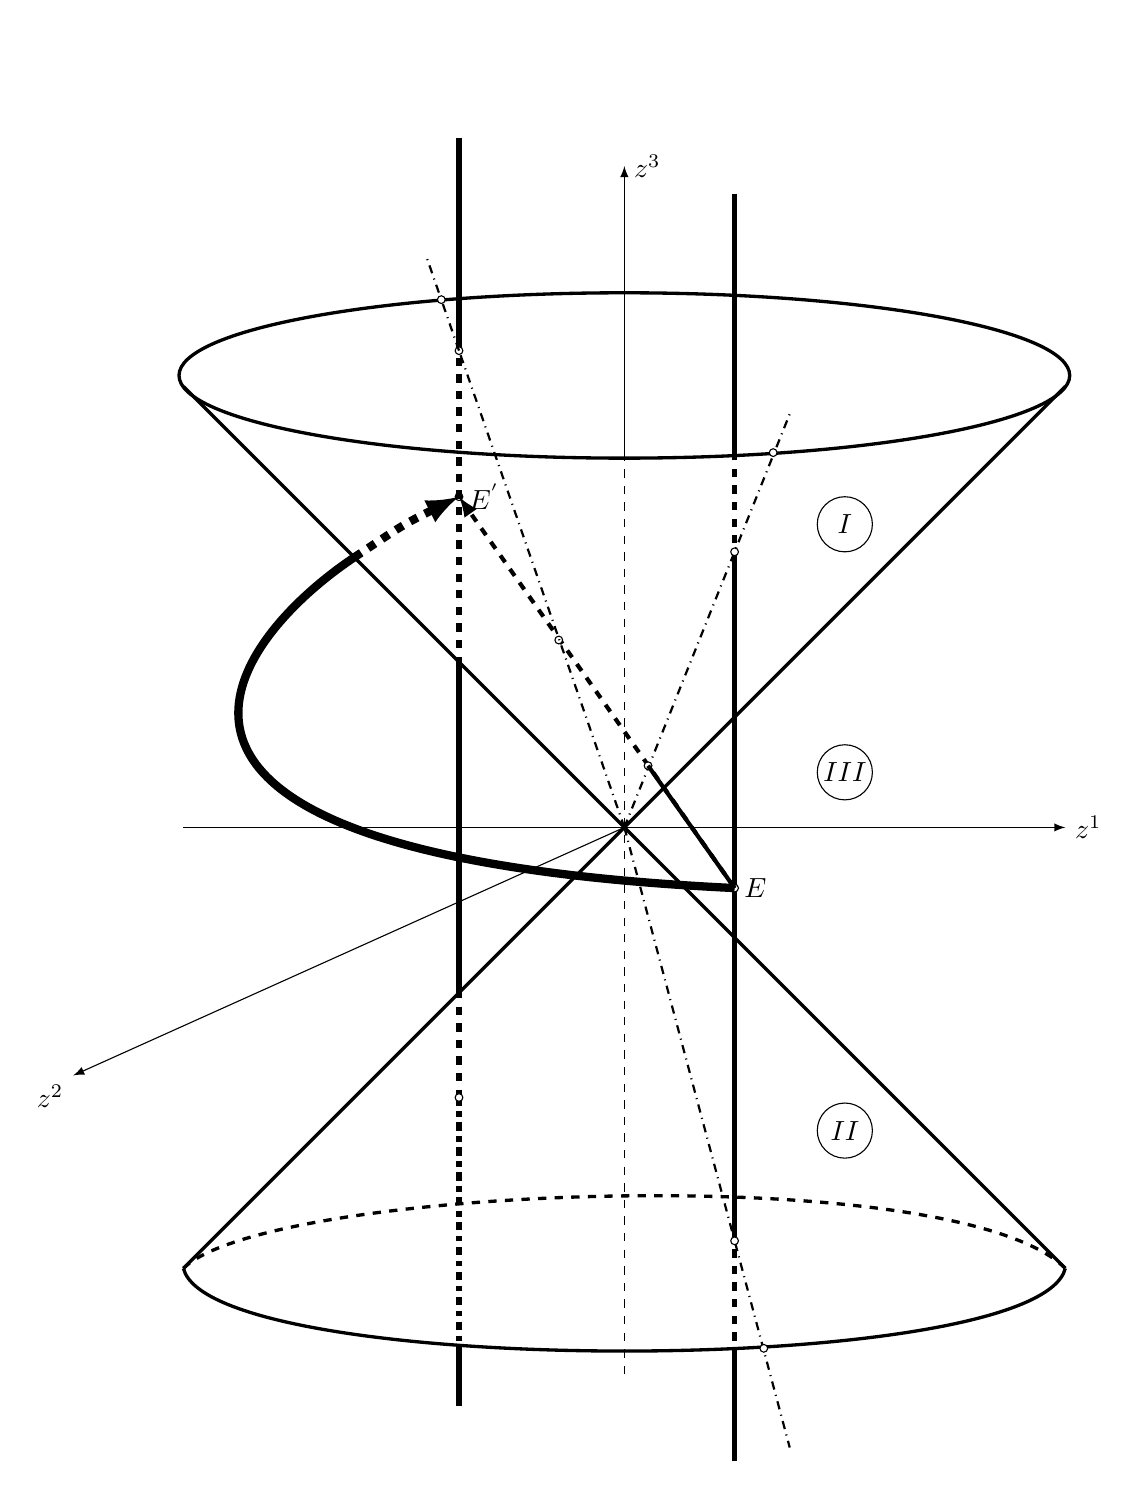
\begin{tikzpicture}[scale=0.70]
\coordinate (v1) at (-8,-0);
\coordinate (v2) at (8,-0) ;
\coordinate (v3) at (0,12) {};
\coordinate (v4) at (0,6.8) {};
\coordinate (v5) at (8,8) {};
\coordinate (v6)  at (0,0) {};
\coordinate (v7) at (-8,-8) {};
\coordinate (v8) at (8,-8) {};
\coordinate (v9) at (-8,8) {};
\coordinate (v10) at (-0,-10) {};
\coordinate (v11)  at (-10,-4.5) {};
\draw[-{latex}]  (v1)-- (v2)node[right] {$z^1$};
\draw  [-{latex}](v4)-- (v3)node[right] {$z^3$};
\draw  [-{latex}](v6)-- (v11)node[{anchor=north east}] {$z^2$};
\draw  [dashed](v4)-- (v10);
\draw[very thick]  (0,8.2) ellipse (8.08 and 1.5);
\draw [very thick] (v6) -- (v5);
\draw [very thick] (v7) -- (v6);
\draw  [very thick](v6) -- (v8);
\draw  [very thick](v6) -- (v9);
\draw[very thick] (-8,-8) .. controls (-7.5,-10) and (7.5,-10) .. (8,-8);
\draw [very thick, dashed,](-8,-8) .. controls (-6.5,-6.5) and (6,-6) .. (8,-8);

\coordinate (p0) at (-3.1,-1.4) {} {};
\coordinate (p1) at (2,-1.5) {} {};
\coordinate (p2) at (2,5) {} {};
\coordinate (p3) at (2,-7.5) {} {};
\coordinate (p4) at (5.5,0) {};

\draw [line width=2] (p2) -- (p1);
\draw [line width=2] (p2) -- (p3);
\coordinate (p5) at (2,6.7) {};
\coordinate (p6) at (2,-9.5) {};
\coordinate (p7)at (2,11.5) {};
\coordinate (p8)  at (2,-11.5) {};
\draw [dashed, line width=2] (p3) -- (p5);
\draw  [dashed, line width=2] (p2) -- (p6);
\draw [ line width=2] (p7) -- (p5);
\draw[ line width=2] (p8) -- (p6);

\coordinate (p9)  at (1.5*2,-1.5*7.5) {};
\coordinate (p10)  at (1.5*2,1.5*5) {};
\draw  [dashdotted,thick](v6) -- (p9);
\draw  [dashdotted,thick](v6) -- (p10);
\coordinate (t1) at (4,5.5) {};
\coordinate (t2) at (4,1) {} ;
\coordinate (t3) at (4,-5.5) {};
\draw[fill=black](t1)node[] {$I$};
\draw[fill=black](t2)node[] {$III$};
\draw[fill=black](t3)node[] {$II$};
\coordinate (t4) at (2.7,6.8) {};
\coordinate (t5) at (2.53,-9.45) {};
\draw[fill=white](t4) circle(2pt);
\draw[fill=white](t5) circle(2pt);

\draw  (t1) ellipse (0.5 and 0.5);
\draw  (t2) ellipse (0.5 and 0.5);
\draw  (t3) ellipse (0.5 and 0.5);
\draw  (-1.5,14.5) ellipse (0 and 0);
\coordinate (q1) at (2,-1.1) {} {} {};
\coordinate (q2) at (-3,6) {} {};
\draw[fill=white](q1) circle(2pt)node[{anchor=west }] {$E^{}$};
\draw[fill=white](q2) circle(2pt)node[{anchor=west }] {$E^{'}$};
\coordinate(q3) at (-4.9,4.9) {};
\draw [line width=3](q1) .. controls (-10.5,-0.5) and (-7,3.5) .. (q3);

\draw [line width=3,dashed, -latex](q3) .. controls (-4,5.5) and (-4,5.5) .. (q2);
\coordinate(s0) at (-3,12.5) {};
\coordinate(s1) at (-3,8.65) {};
\coordinate(s2) at (-3,-4.9) {};
\coordinate(s3) at (-3,2.95) {};
\coordinate(s4) at (-3,-2.95) {};
\coordinate(s5) at (-3,-9.5) {};
\coordinate(s6) at (-3,-10.5) {};
\coordinate(s7) at (-3*1.2,8.65*1.2) {};
\coordinate(s8) at (-3*1.107,8.65*1.107) {};
\draw [line width=2] (s1) -- (s0);
\draw [line width=2,dashed] (s3) -- (s1);
\draw [line width=2] (s3) -- (s4);
\draw [line width=2,dashdotted] (s2) -- (s5);
\draw [line width=2,dashed] (s4) -- (s2);
\draw [line width=2] (s5) -- (s6);
\draw[fill=white](s1) circle(2pt);
\draw[fill=white](s2) circle(2pt);
\draw[fill=white](p3) circle(2pt);
\draw[fill=white](p2) circle(2pt);
\draw [line width=1.5, dashed,-latex] (q1) -- (q2);
\coordinate(w0) at (-1*1.19,3.4) {} {};
\coordinate(w1)  at (0.43,1.12) {};
\draw[fill=white](w0) circle(2pt);
\draw[fill=white](w1) circle(2pt);
\draw  [dashdotted,thick](v6) -- (s1);
\draw  [dashdotted,thick](s1) -- (s7);
\draw[fill=white](s8) circle(2pt);
\draw [line width=1.5, ] (w1) -- (q1);
\end{tikzpicture}
\caption{Travelling between two points in region III (present) in a  $V_3$ space-time manifold}
\label{fig:fig_p96_3415_b}
\end{figure}
\end{comment}
$$\blacklozenge$$
\newpage

\section{p133 - Exercise}
\begin{tcolorbox}
In a space of two dimensions prove the relation
$$\mathbf{4.318.}\spatie \in_{mp}\in_{mq} = \delta_{pq}$$
\end{tcolorbox}
Suppose $p=q$, then in the summation the term is $0$ if $m=p=q$ and the remaining term is $1\times 1$ or $-1\times -1$ giving indeed $\delta_{pq}=1$.\\ 
If  $p\neq q$ we get either $m=p$ or $m=q$ in each term of the summation and hence all terms vanish.
$$\blacklozenge$$
\newpage

\section{p135 - Exercise}
\begin{tcolorbox}
Write out the six independent non-zero components of $P_{mn}$ as given by $\mathbf{4.324.}$
\end{tcolorbox}
We have 
\begin{align}
\mathbf{4.324.}\spatie P_{mn}= \in_{mnrs}X^rY^s\\
\text{with}\quad \spatie m=n \quad \Rightarrow \quad P_{mn}= 0
\end{align}
So, the six independent components are in the set $\{mn\}= \left\{12,13,14,23,24,34 \right\}$ as $P_{nm}=-P_{mn}$.
\begin{align}
&\left\{\begin{array}{l}\\
P_{12} = \in_{1234}X^3Y^4+\in_{1243}X^4Y^3\\\\
P_{13} = \in_{1324}X^2Y^4+\in_{1342}X^4Y^2\\\\
P_{14} = \in_{1423}X^2Y^3+\in_{1432}X^3Y^2\\\\
P_{23} = \in_{2314}X^1Y^4+\in_{2341}X^4Y^1\\\\
P_{24} = \in_{2413}X^1Y^3+\in_{2431}X^3Y^1\\\\
P_{34} = \in_{3412}X^1Y^2+\in_{3421}X^2Y^1\\\\
\end{array}\right.\\
&\left\{\begin{array}{l}\\
P_{12} = X^3Y^4-X^4Y^3\\\\
P_{13} = -X^2Y^4+X^4Y^2\\\\
P_{14} = X^2Y^3-X^3Y^2\\\\
P_{23} = X^1Y^4-X^4Y^1\\\\
P_{24} = -X^1Y^3+X^3Y^1\\\\
P_{34} = X^1Y^2-X^2Y^1\\\\
\end{array}\right.
\end {align}
$$\blacklozenge$$
\newpage

\section{p135 - Exercise}
\begin{tcolorbox}
Translate the well-known vector relations
$$A\times (B\times C)= B(A.  C)-C(A.B)$$
$$\nabla \times (\nabla \times V)= \nabla (\nabla .  V )-\nabla^2V$$
into Cartesian tesnor form, and prove the by use of $4.329$.
\end{tcolorbox}
We have 
\begin{align}
\mathbf{4.329.}\spatie \in_{mrs}\in_{mpq} = \delta_{rp}\delta_{sq}-\delta_{rq}\delta_{sp}
\end{align}
The first identity
\begin{align}
A\times (B\times C)= B(A.  C)-C(A.B)\\
\Leftrightarrow\spatie \in_{npm}\in_{mrs}A_p B_r C_s = A_p\left(B_n C_p-C_n B_p\right)
\end{align}
Indeed,
\begin{align}
(B\times C)_m &= \in_{mrs}B_rC_s\\
\Rightarrow\spatie \left(A\times (B\times C)\right)_n &=\in_{npm}A_p \in_{mrs}B_rC_s\\
&=-\in_{mpn}\in_{mrs}A_p \in_{mrs}B_r C_s\\
&= -\delta_{pr}\delta_{ns}A_pB_rC_s+\delta_{ps}\delta_{nr}A_pB_rC_s\\
&= A_pB_nC_p-A_pB_pC_n\\
\Leftrightarrow\spatie & B(A.  C)-C(A.B)
\end{align}
The second identity
\begin{align}
\nabla \times (\nabla \times V)&= \nabla (\nabla .  V )-\nabla^2V\\
\Leftrightarrow \spatie \in_{nrm}\in_{mpq}V_{q,pr} &= V_{p,pn}- V_{n,pp}
\end{align}
Indeed,
\begin{align}
\left(\nabla \times V\right)_m &= \in_{mpq}V_{q,p}\\
\Rightarrow\spatie \left(\nabla  \times (\nabla \times V)\right)_n &=\in_{nrm}\left(\in_{mpq}V_{q,p}\right)_{,r}\\
 &=\in_{nrm}\in_{mpq}V_{q,pr}\\
 &=\delta_{rq}\delta_{np}V_{q,pr}-\delta_{pr}\delta_{nq}V_{q,pr}\\
 &= V_{p,pn}-V_{n,pp}
\end{align}
We have also
\begin{align}
\left(\nabla V\right) &= V_{p,p}\\
\Rightarrow\spatie \left(\nabla (\nabla .  V )\right)_n &= \left(V_{p,p}\right)_n\\
&= V_{p,pn}
\end{align}
and 
\begin{align}
\nabla^2 V_n  & \equiv  V_{n,pp} \\
\Rightarrow\spatie \left(\nabla (\nabla .  V )\right)_n- \nabla^2 V_n &= V_{p,pn}- V_{n,pp}
\end{align}
which corresponds to (15).
So the tensor expression in Cartesian tensor form can be written as 
$$\in_{nrm}\in_{mpq}V_{q,pr} = V_{p,pn}- V_{n,pp}$$

$$\blacklozenge$$
\newpage

\section{p139 - Exercise 1.}
\begin{tcolorbox}
Show that, in a 3-space of constant curvature $-\frac{1}{R^2}$ and positive definite metric form, the line element in polar coordinate is 
$$ds^2= dr^2+R^2\sinh^2\left(\frac{r}{R}\right)\left(d\theta^2+\sin^2\theta d\phi^2\right)$$
\end{tcolorbox}
We have by $4.120c$
\begin{align}
X_r \eta^r &= A\sinh \left(s\sqrt{-\epsilon K}\right)
\end{align}
We choose $N$ different $X^{(k)}_r$ $(k= 1,2,\dots, N)$ which are orthonormal.
Applying $(1)$ $N$ times with the different $X^{(k)}_r$ $(k= 1,2,\dots, N)$, we get
\begin{align}
X^{(k)}_r \eta^r &= A^{(k)}\sinh \left(s\sqrt{-\epsilon K}\right)
\end{align}
But as the $X^{(k)}_r$ are orthonormal and are used as a basis at the considered point of the geodesic we have 
\begin{align}
X^{(k)}_r &= \delta^k_r
\end{align}
So, $(2)$ becomes
\begin{align}
\eta^k &= A^{(k)}\sinh \left(s\sqrt{-\epsilon K}\right)
\end{align}
which are the components of the displacement vector in the orthonormal basis. By $\mathbf{2.301.}$ :
\begin{align}
Y^2 &= \epsilon a_{mn} Y^m Y^n\\
\Rightarrow \spatie \eta^2 &= \epsilon a_{mn} A^{(m)} A^{(n)}\sinh^2 \left(s\sqrt{-\epsilon K}\right)\\
\Rightarrow \spatie \eta &= C\left|\sinh \left(s\sqrt{-\epsilon K}\right)\right|\\
\text{with}\spatie C&= \sqrt{\left|\epsilon a_{mn} A^{(m)} A^{(n)}\right|}
\end{align}
As $\epsilon =1$ (positive-definite metric) and $K=-\frac{1}{R^2}$
we have
\begin{align}
\eta &= C\left|\sinh \left(\frac{s}{R}\right)\right|
\end{align}
From this and using the very same reasoning from $4.126.$ to $4.130.$ (pages 117-119) we get 
$$ds^2= dr^2+R^2\sinh^2\left(\frac{r}{R}\right)\left(d\theta^2+\sin^2\theta d\phi^2\right)$$
$$\blacklozenge$$
\newpage


\section{p139 - Exercise 2.}
\begin{tcolorbox}
Show that the volume of an antipodal 3-space of positive-definite metric form and positive constant curvature $\frac{1}{R^2}$ is $2\pi^2R^3$. (Use the equation 4.130. to find the area of a sphere $r= \text{constant}$ in polar coordinates. Multiply by $dr$ and integrate for $0\leq r \leq \pi R$ to get the volume). What is the volume if the space is polar?
\end{tcolorbox}
We have  $4.130$
\begin{align}
ds^2= dr^2+R^2\sin^2\left(\frac{r}{R}\right)\left(d\theta^2+\sin^2\theta d\phi^2\right)
\end{align}
Having a positive-definite metric form, the space can be locally considered as Euclidean and an elementary area of a  surface with constant $r (\rightarrow dr=0)$ can be calculated as $dS=ds_{d\theta=0}ds_{d\phi=0}$ and get by (1)
\begin{align}
dS &= R^2\sin^2\left(\frac{r}{R}\right)\sin\theta d\phi d\theta\\
\Rightarrow\spatie\frac{S}{8} &= R^2\sin^2\left(\frac{r}{R}\right)\int^{\frac{\pi}{2}}_{0}\int^{\frac{\pi}{2}}_{0} \sin\theta d\phi d\theta\\ 
&= R^2\sin^2\left(\frac{r}{R}\right)\frac{\pi}{2} \left.\left(-\cos\theta \right)\right|^{\frac{\pi}{2}}_{0}\\
\Rightarrow\spatie S&= 4\pi R^2\sin^2\left(\frac{r}{R}\right)
\end{align}
We see that the area is a cyclic function of $r$ having zeros' at $r= k\frac{\pi}{R }, k=1,2,\dots$
\begin{figure}[H]
\begin{center}
\begin{tikzpicture}[]
    \begin{axis}[
    domain = 0:2.5*pi,
    samples = 201,
    axis on top = true,
    grid =none,
    grid style = {dashed, line width=.1pt, draw=gray!30, 
    /pgfplots/on layer=axis background},
    		ytick=\empty,
		xtick=\empty,
		xmin=-0,
		xmax=9,
		ymin=0,
		ymax=1.5,
]
\addplot+[no marks, color=black] {(sin(deg(x)))^2};
\node[{anchor=south east}] at (0,10){$\phi_0$};
\end{axis}
\coordinate(0) at (0,0);
\node[{anchor=north east }] at (0){$0$};
\coordinate(p1) at (2.7,0);
\node[{anchor=north east }] at (p1){$\pi$};
\coordinate(p2) at (2*2.5,0);
\node[{anchor=north east }] at (p2){$2\pi$};
\end{tikzpicture}
\caption{Area of an antipodal 3-space of positive-definite metric form}
\label{fig:fig_p138_Ex2}
\end{center}
\end{figure}
So, there are good reasons to restrict $r$ to $[0,\pi R]$ as otherwise all space of that type would have infinite volume, whatever it's curvature. So, we get as volume 
\begin{align}
V &= 4\pi R^2\int^{\pi R}_{0}\sin^2\left(\frac{r}{R}\right)dr\\
&= 4\pi R^3\int^{\pi R}_0\sin^2\left(\frac{r}{R}\right)d\left(\frac{r}{R}\right)\\
&= 4\pi R^3\left.\left( \half x - \frac{1}{4}\sin2x \right)\right|^{\pi}_0\\
&= 2\pi^2 R^3
\end{align}
Fo a polar space, the volume would be half of that of an antipodal one (with same curvature of course) as in (3) we would consider only 4 quadrants instead of 8.
$$\blacklozenge$$
\newpage


\section{p139 - Exercise 3.}
\begin{tcolorbox}
By direct calculation of the tensor $R_{rsmn}$ verify that $\mathbf{4.130.}$ is the metric form of a space of constant curvature.
\end{tcolorbox}
We have  $4.130$
\begin{align}
ds^2&= dr^2+R^2\sin^2\left(\frac{r}{R}\right)\left(d\theta^2+\sin^2\theta d\phi^2\right)\\
\Rightarrow\spatie &
\ (a_{mn}) = \begin{pmatrix}
 1& 0 & 0\\
0 & R^2\sin^2\left(\frac{r}{R}\right) & 0 \\
0 & 0 & R^2\sin^2\left(\frac{r}{R}\right)\sin^2\theta \\
\end{pmatrix}
\end{align}
Now for $R_{rsmn}$ we refer to exercise 7 page 109 of chapter 3, where the curvature tensor was calculated for a general case of the form 
$$ ds^2= (h_1dx^1)^2+(h_2dx^2)^2+(h_3dx^3)^2$$ where $h_1, h_2, h_3$ are functions of the three coordinates.
We have then for our case
\begin{align}
\left\{\begin{array}{l}
h_1 = 1\\\\
h_2 = R\sin\left(\frac{r}{R}\right)\\\\
h_3 = R\sin\left(\frac{r}{R}\right)\sin\theta\\\\
\end{array}\right.
\end{align}
In the exercise we got for the non-vanishing curvature tensors
\begin{align}
R_{1212}&=
-h_2\partial_{11}^2(h_2)-h_1\partial_{22}^2(h_1)
+\frac{h_2}{h_1}\partial_1 h_1\partial_1 h_2+\frac{h_1}{h_2}\partial_2 h_1\partial_2 h_2-\frac{h_1 h_2}{h_3^2}\partial_3 h_1\partial_3 h_2\\
R_{2323}&=
-h_3\partial_{22}^2(h_3)-h_2\partial_{33}^2(h_2)
+\frac{h_3}{h_2}\partial_2 h_2\partial_2 h_3+\frac{h_2}{h_3}\partial_3 h_2\partial_3 h_3-\frac{h_2 h_3}{h_1^2}\partial_1 h_2\partial_1 h_3\\
R_{1313}&=
-h_3\partial_{11}^2(h_3)-h_1\partial_{33}^2(h_1)
+\frac{h_3}{h_1}\partial_1 h_1\partial_1 h_3+\frac{h_1}{h_3}\partial_3 h_1\partial_3 h_3-\frac{h_1 h_3}{h_2^2}\partial_2 h_1\partial_2 h_3
\end{align}
\begin{align}
R_{1213}&=-h_1\partial_{32}^2(h_1)+\frac{h_1}{h_3}\partial_2 h_3\partial_3 h_1+\frac{h_1}{h_2}\partial_2 h_1\partial_3 h_2\\
R_{1223}&=h_2\partial_{31}^2(h_2)-\frac{h_2}{h_1}\partial_1 h_2\partial_3 h_1-\frac{h_2}{h_3}\partial_3 h_2\partial_1 h_3\\
R_{1323}&=
-h_3\partial_{21}^2(h_3)+\frac{h_3}{h_1}\partial_1 h_3\partial_3 h_1+\frac{h_3}{h_2}\partial_2 h_3\partial_1 h_2
\end{align}
Clearly $\partial_{k}^2(h_1)=0$ and $\partial_{mn}^2(h_1)=0$ and considering $h_2 = h_2(r), \ h_3 = h_3(r,\theta)$
we can simplify 
\begin{align}
R_{1212}&=
-h_2\partial_{11}^2(h_2)\\
R_{2323}&=
-h_3\partial_{22}^2(h_3)
-\frac{h_2 h_3}{h_1^2}\partial_1 h_2\partial_1 h_3\\
R_{1313}&=
-h_3\partial_{11}^2(h_3)
\end{align}
\begin{align}
R_{1213}&=0\\
R_{1223}&=0\\
R_{1323}&=
-h_3\partial_{21}^2(h_3)+\frac{h_3}{h_2}\partial_2 h_3\partial_1 h_2
\end{align}
with 
\begin{align}
\left\{\begin{array}{l}
\partial_1 h_2=\cos\left(\frac{r}{R}\right)\\\\
\partial_1 h_3=\cos\left(\frac{r}{R}\right)\sin\theta\\\\
\partial_2 h_3=R\sin\left(\frac{r}{R}\right)\cos\theta\\\\
\partial^2_{11} h_2=-\frac{1}{R}\sin\left(\frac{r}{R}\right)\\\\
\partial^2_{11} h_3=-\frac{1}{R}\sin\left(\frac{r}{R}\right)\sin\theta\\\\
\partial^2_{21} h_3=\cos\left(\frac{r}{R}\right)\cos\theta\\\\
\partial^2_{22} h_3=-R\sin\left(\frac{r}{R}\right)\sin\theta\\\\
\end{array}\right.
\end{align}
giving
\begin{align}
R_{1212}&=
\sin^2\left(\frac{r}{R}\right)\\
R_{2323}&=
R^2\sin^2\left(\frac{r}{R}\right)\sin^2\theta 
-R^2\sin^2\left(\frac{r}{R}\right)\sin^2\theta\cos^2\left(\frac{r}{R}\right)\\
&= R^2\sin^4\left(\frac{r}{R}\right)\sin^2\theta\\
R_{1313}&=\sin^2\left(\frac{r}{R}\right)\sin^2\theta\\
R_{1213}&=0\\
R_{1223}&=0\\
R_{1323}&=
-R\sin\left(\frac{r}{R}\right)\sin\theta\cos\left(\frac{r}{R}\right)\cos\theta+\sin\theta R\sin\left(\frac{r}{R}\right)\cos\theta\cos\left(\frac{r}{R}\right)\\&=0
\end{align}
and considering the symmetries
\begin{align}
R_{1212}&=-R_{1221}=-R_{2112}=
\sin^2\left(\frac{r}{R}\right)\\
R_{2323}&=-R_{2332}=-R_{3223}= R^2\sin^4\left(\frac{r}{R}\right)\sin^2\theta\\
R_{1313}&=-R_{1331}=-R_{3113}=\sin^2\left(\frac{r}{R}\right)\sin^2\theta\\
\end{align}
By $\mathbf{4.114.}$
\begin{align}
R_{rsmn}&= K\left(a_{rm}a_{sn}-a_{rn}a_{sm}\right)\\
\Rightarrow\spatie &\left\{\begin{array}{l}
R_{1212}= K\left(a_{11}a_{22}-a_{12}a_{21}\right)\\
R_{2323}= K\left(a_{22}a_{33}-a_{23}a_{32}\right)\\
R_{1313}= K\left(a_{11}a_{33}-a_{13}a_{31}\right)
\end{array}\right.\\
\Rightarrow\spatie &\left\{\begin{array}{l}
R_{1212}= K R^2\sin^2\left(\frac{r}{R}\right)\\
R_{2323}= K R^2\sin^2\left(\frac{r}{R}\right)R^2\sin^2\left(\frac{r}{R}\right)\sin^2\theta\\
R_{1313}= K R^2\sin^2\left(\frac{r}{R}\right)\sin^2\theta\\
\end{array}\right.\\
\Rightarrow\spatie &\left\{\begin{array}{l}
R_{1212}= K R^2\sin^2\left(\frac{r}{R}\right)\\
R_{2323}= K R^4\sin^4\left(\frac{r}{R}\right)\sin^2\theta\\
R_{1313}= K R^2\sin^2\left(\frac{r}{R}\right)\sin^2\theta\\
\end{array}\right.
\end{align}
 replacing (25), (26) and (27) in (32) we get
 \begin{align}
\left\{\begin{array}{l}
\sin^2\left(\frac{r}{R}\right)= K R^2\sin^2\left(\frac{r}{R}\right)\\
R^2\sin^4\left(\frac{r}{R}\right)\sin^2\theta= K R^4\sin^4\left(\frac{r}{R}\right)\sin^2\theta\\
\sin^2\left(\frac{r}{R}\right)\sin^2\theta= K R^2\sin^2\left(\frac{r}{R}\right)\sin^2\theta\\
\end{array}\right.
\end{align}
giving indeed for the three curvature tensors $K=\frac{1}{R^2}$\\
With this, the question of the  exercise is answered but we go a little bit further and investigate for this practical case the equations of $\mathbf{4.115.}$ and  calculate $R=a^{mn}R_{mn}$. With $R$, the curvature invariant. To avoid confusion with the curvature $R$ itself we use $\mathfrak{R}$ for the curvature invariant.\\
As the metric tensor is diagonal:

\begin{align}
\mathfrak{R}=a^{11}R_{11}+a^{22}R_{22}+a^{33}R_{33}\\
\end{align}
and 
\begin{align}
R_{mn}&= a^{sn}R_{srmn}\\
\Rightarrow\spatie &
\left\{\begin{array}{l}
R_{11} = a^{11}R_{1111}+a^{22}R_{2112}+a^{33}R_{3113}\\\\
R_{22} = a^{11}R_{1221}+a^{22}R_{2222}+a^{33}R_{3223}\\\\
R_{33} = a^{11}R_{1331}+a^{22}R_{2332}+a^{33}R_{3333}\\\\
\end{array}\right.\\
\Rightarrow\spatie &\left\{\begin{array}{l}
R_{11} = -a^{22}\sin^2\left(\frac{r}{R}\right)-a^{33}\sin^2\left(\frac{r}{R}\right)\sin^2\theta\\\\
R_{22} = -a^{11}\sin^2\left(\frac{r}{R}\right)-a^{33}R^2\sin^4\left(\frac{r}{R}\right)\sin^2\theta\\\\
R_{33} = -a^{11}\sin^2\left(\frac{r}{R}\right)\sin^2\theta-a^{22}R^2\sin^4\left(\frac{r}{R}\right)\sin^2\theta\\\\
\end{array}\right.\\
\Rightarrow\spatie &\left\{\begin{array}{l}
R_{11} = -\frac{\sin^2\left(\frac{r}{R}\right)}{R^2\sin^2\left(\frac{r}{R}\right)}-\frac{\sin^2\left(\frac{r}{R}\right)\sin^2\theta}{R^2\sin^2\left(\frac{r}{R}\right)\sin^2\theta}\\\\
R_{22} = -\sin^2\left(\frac{r}{R}\right)-\frac{R^2\sin^4\left(\frac{r}{R}\right)\sin^2\theta}{R^2\sin^2\left(\frac{r}{R}\right)\sin^2\theta}\\\\
R_{33} = -\sin^2\left(\frac{r}{R}\right)\sin^2\theta-\frac{R^2\sin^4\left(\frac{r}{R}\right)\sin^2\theta}{R^2\sin^2\left(\frac{r}{R}\right)}\\\\
\end{array}\right.
\end{align}
giving
\begin{align}
\left\{\begin{array}{l}
R_{11} = -\frac{2}{R^2}\\\\
R_{22} = -2\sin^2\left(\frac{r}{R}\right)\\\\
R_{33} = -2\sin^2\left(\frac{r}{R}\right)\sin^2\theta\\\\
\end{array}\right.
\end{align}
hence
\begin{align}
\mathfrak{R}&=a^{11}R_{11}+a^{22}R_{22}+a^{33}R_{33}\\
\Rightarrow\spatie R&= -\frac{2}{R^2}-2\frac{\sin^2\left(\frac{r}{R}\right)}{R^2\sin^2\left(\frac{r}{R}\right)}-2\frac{\sin^2\left(\frac{r}{R}\right)\sin^2\theta}{R^2\sin^2\left(\frac{r}{R}\right)\sin^2\theta }\\
\mathfrak{R}&= -\frac{6}{R^2}
\end{align}
The equations in (40) and (43) are indeed in accordance with $\mathbf{4.115}$ .
$$\blacklozenge$$
\newpage

\section{p139 - Exercise 4}
\begin{tcolorbox}

\end{tcolorbox}

$$\blacklozenge$$
\newpage
%\setcounter{chapter}{4}
\chapter{Applications to Classical Mechanics}
\pagebreak[4]
\section{p153 - Exercise}
\begin{tcolorbox}
If $\mu^{\alpha}$ are the contravariant components of a unit vector in a surface $S$, show that $\mu^{\alpha}f_{\alpha}$ is the physical component of acceleration in the direction tangent to $S$ defined by $\mu^{\alpha}$.
\end{tcolorbox}
As we are in an Euclidean space we can interpret $a_{mn}\mu^{\alpha}f^{\alpha}$ as $\left|\mu\right|\left|f\right|\cos\theta $ with $\theta$ the angle between the two vectors. As $\left|\mu\right|=1$ we have
\begin{align}
a_{mn}\mu^{\alpha}f^{\alpha}&= \mu^{\alpha}f_{\alpha}\\
&= \left|f\right|\cos\theta 
\end{align}
which is the projection of the vector $f$ on the unit vector $\mu$.
$$\blacklozenge$$
\newpage

\section{p154 - Clarification to 5.226.}
\begin{tcolorbox}
$$\mathbf{\text{5.226.}\spatie v\dv{v}{s}=0,\quad \overline{\kappa}v^2=0}$$
Assuming that the particle is not at rest $v\ne 0$, and therefore $\overline{\kappa}=0$. \textit{\textbf{Since this implies that the curve is a geodesic}...}
\end{tcolorbox}
The assertion in bold is a direct consequence $$\mathbf{\text{2.513.}}\spatie \frac{\delta \dv{x^r}{s}}{\delta s}=0$$ 
As in $ \mathbf{5.233}$ we have $\frac{\delta \lambda^{\alpha}}{\delta s}=\frac{\delta \dv{x^{\alpha}}{s}}{\delta s}=0$, the considered curve follows the geodesic curve.
$$\blacklozenge$$
\newpage

\section{p155 - Exercise}
\begin{tcolorbox}
Show that in relativity the force $4$-vector $X^r$ lies along the first normal of the trajectory in space-time. Express the first curvature in terms of the proper mass $m$ of the particle and the magnitude $X$ of $ X^r$.
\end{tcolorbox}
Let us recall the first Frenet formula $\mathbf{2.705}$ without forgetting that the metric form is not positive-definite, $$\frac{\delta \lambda^r}{\delta s}=\kappa\nu^r,\quad \epsilon_{(1)}\nu_n\nu^n=1$$ As $\mathbf{5.299}$ $$m\frac{\delta \lambda^r}{\delta s}=X^r$$ it is clear that $X^r = m\kappa\nu^r$ and is collinear with the first normal.
\begin{align}
X^r &= m\kappa\nu^r\\
\times \quad a_{mr}X^m\quad\Rightarrow\spatie \underbrace{a_{mr}X^mX^r}_{=\left(X^1\right)^2+\left(X^2\right)^2+\left(X^3\right)^2-\left(X^4\right)^2} &= m\kappa \underbrace{a_{mr}\nu^m\nu^r}_{= \epsilon_{(1)}}
\end{align}
\textbf{$$\Rightarrow\spatie \kappa = \epsilon_{(1)}\frac{\left(X^1\right)^2+\left(X^2\right)^2+\left(X^3\right)^2-\left(X^4\right)^2}{m}
$$}
$$\blacklozenge$$
\newpage


\section{p156 - Clarification}
\begin{tcolorbox}
Interpretation of 
$$\mathbf{5.231.}\spatie M_{rs}=\epsilon_{rsn}M_n=z_rF_s-z_sF_r$$
\end{tcolorbox}
What do the $M_{rs}$ represent?
\begin{figure}[H]

\begin{tikzpicture}[scale=0.75]
\tikzstyle{left-hand-mirror} = [
    draw,
    postaction=decorate, 
    decoration={
        markings,
        mark=between positions 0.015 and 0.98 step 0.1072 with {\draw (0,0)--(60:3pt);}
    }
]  
\coordinate (O) at (0,0);
\coordinate (X) at (-5,-5);
\coordinate (Y) at (10,0);
\coordinate (Z) at (0,10);
\draw [-{Latex[length=3mm]}] (O) -- (X);
\draw [-{Latex[length=3mm]}] (O) -- (Y);
\draw [-{Latex[length=3mm]}] (O) -- (Z);
\node[label=north west:$z_1$] at (X) {};
\node[label=north east:$z_2$] at (Y) {};
\node[label=north west:$z_3$] at (Z) {};
\coordinate (P) at (5,3);
\draw [-{Latex[length=3mm]},ultra thick] (O) -- (P);
\node[label=north west:$P$] at (P) {};
\coordinate (F) at (8,7) {};
\draw [-{Latex[length=3mm]}, ultra thick] (P) -- (F);
\node[above right] at (F) {$\overrightarrow{F}$};
\coordinate (Fp) at (8-5,7-3) {};
\draw [-{Latex[length=3mm]},dashdotted,ultra thick] (O) -- (Fp);
\node[above right,] at (Fp) {$\overrightarrow{F^{'}}$};
\coordinate (Px) at (-2,-2) {};
\coordinate (Py) at (6.8,0) {};
\node[label=north west:$P_1$] at (Px) {};
\node[label=north west:$P_2$] at (Py) {};
\coordinate (Pp) at (5,-2) {};
\draw [dashed] (Pp) -- (P);
\draw [dashed] (Pp) -- (Px);
\draw [dashed] (Pp) -- (Py);
\coordinate (Fpp) at (3,-1) {};
\coordinate (Fx) at (-1,-1) {} {};
\coordinate (Fy) at (4,0) {} {};
\node[label=north west:$F_1$] at (Fx) {};
\node[label=north west:$F_2$] at (Fy) {};
\draw[fill = black]  (Fx) circle (0.1);
\draw[fill = black]  (Fy) circle (0.1);
\draw [dashed] (Fp) -- (Fpp);
\draw [dashed] (Fpp) -- (Fx);
\draw [dashed] (Fpp) -- (Fy);

\coordinate (Fppp) at (6,-1) {} {};
\coordinate (Pppp) at (2,-2) {} {} {};
\node[{anchor=north west }] at (Fppp) {$\overrightarrow{F_1}$};
\node[{anchor=south east }] at (Pppp) {$\overrightarrow{F_2}$};
\draw [-{Latex[length=3mm]}, ultra thick] (O) -- (Px);
\draw [-{Latex[length=3mm]},ultra thick] (O) -- (Py);
\draw [-{Latex[length=3mm]}, ultra thick] (Px) -- (Pppp);
\draw [-{Latex[length=3mm]},ultra thick] (Py) -- (Fppp);
%\node[label=north west:$K$] at (Fppp) {};
%\node[label=north west:$S$] at (Pppp) {};
\draw [dashed] (Fp) -- (Fpp);
\draw [dashed] (Fppp) -- (Fx);
\draw [dashed] (Pppp) -- (Fy);
%\filldraw[ultra thick, gray!10] (Px) -- (Pppp) -- (Fy) -- (O) -- (Px) -- cycle;
%\filldraw[ultra thick,gray!20] (Fx) -- (Fppp) -- (Py) -- (O) -- (Px) -- cycle;
%\draw[ultra thick, gray!80] (Px) -- (Pppp) -- (Fy) -- (O) -- (Px) -- cycle;
%\draw[ultra thick,gray!80] (Fx) -- (Fppp) -- (Py) -- (O) -- (Px) -- cycle;
\coordinate (Vp1) at (0,6) {} {};
\coordinate (Vp2) at (0,9) {} {} {};
\draw [-{Latex[length=3mm]}, ultra thick] (O) -- (Vp1);
\draw [-{Latex[length=3mm]}, ultra thick] (O) -- (Vp2);
\node[{anchor=north west }] at (Vp1) {$\overrightarrow{P_1}\times\overrightarrow{F_2}$};
\node[{anchor=north west }] at (Vp2) {-$\overrightarrow{P_2}\times\overrightarrow{F_1}$};
\draw[fill=white]  (Py) circle (0.1);
\draw[fill=white]  (Px) circle (0.1);
\draw[fill=white]  (P) circle (0.1);
\draw[decoration={markings, mark=at position 0.1 with {\arrow[scale = 1.5]{latex[]}}},
    postaction={decorate}](0,4.3) ellipse (1 and 0.2);
    \draw[decoration={markings, mark=at position 0.1 with {\arrow[scale = 1.5]{latex[reversed]}}},
    postaction={decorate}](0,7.3) ellipse (1 and 0.2);
 \coordinate (Qx) at (3.9,1.7) {} {};
\coordinate (Qy) at (8,3) {} {} {};
\draw [-{Latex[length=3mm]},dotted, ultra thick] (P) -- (Qx);
\draw [-{Latex[length=3mm]},dotted, ultra thick] (P) -- (Qy);
\node[{anchor=north west }] at (Qx) {$\overrightarrow{F_1}$};
\node[{anchor=north west }] at (Qy) {$\overrightarrow{F_2}$};
\end{tikzpicture}
\caption{Interpretation of the tensor moment $M_{12}$}
\label{fig:fig_p156_5320}
\end{figure}
Let's consider a mass point $P$ on which a force $\overrightarrow{F}$ is acting. The force has components $\left(F_x,F_y,F_z\right)$ in the  space $V^{'}_3$ (which is by the way not the space $V_3$ of the considered mass point).\\
Let's investigate the element $M_{12}$ of the \textit{tensor moment}.\\
$P_1F_2\overrightarrow{e_3}$ is the vector product $\overrightarrow{P_1}\times\overrightarrow{F_2}$ and is as such the torque of the component $F_2$ of $\overrightarrow{F}$ acting on the mass point situated at $P_1$. The origin being fixed, $\overrightarrow{F_2}$ tries to move $P_1$, clockwise along the $z_3$ axis. The same is true for the component $\overrightarrow{F_1}$ acting on the mass point situated at $P_2$, and is represented here by the vector $- \overrightarrow{P_2}\times\overrightarrow{F_1}$ ($\overrightarrow{F_1}$ tries to move  $P_2$, counter clockwise along the $z_3$ axis). \\
Hence, $P_1F_2-P_2F_1$ is the net force trying to move the point $P$ along the $z_3$ axis (i.e. in the plane $\parallel$ with the $z_3=0$ plane).
$$\blacklozenge$$
\newpage


\section{p156 - Clarification}
\begin{tcolorbox}
$$\mathbf{5.234.}\spatie \dv{h_r}{t}= M_r$$
\end{tcolorbox}
\begin{align}
h_r &= m\epsilon_{rmn}z_mv_n\\
\Rightarrow \spatie \dv{h_r}{t} &= m\epsilon_{rmn}\dv{z_m}{t} v_n+m\epsilon_{rmn}z_m\dv{v_n}{t}\\
&= m\underbrace{\epsilon_{rmn}v_m v_n}_{=0}+\underbrace{\epsilon_{rmn}z_mF_n}_{=M_r}\\
&=M_r
\end{align}
$$\blacklozenge$$
\newpage



\section{p158-159 - Clarification}
\begin{tcolorbox}
$$\mathbf{5.313.}\spatie \omega_{rs}= -\omega_{sr}$$ From 5.310 and the vector character of $v_r$ and $z_r$ (for transformations which do not change the origin), \textbf{it follows that $\omega_{rs} $ is a Cartesian tensor of second order}.
\end{tcolorbox}
Be 
\begin{align}
v^{}_r = -\omega^{}_{rn}z^{}_n
\end{align}
Considering orthogonal transformation in a flat space $z^{'}_m = A_{mr}z^{}_r+B_m$ with  $B_m=0$ as we consider only transformations which do not change the origin. Differentiation with the parameter $t$ gives 
\begin{align}
v^{'}_m &= A_{mr}v^{}_r\\
&= -\omega^{}_{rn}A_{mr}z^{}_n\\
\end{align}
But $z^{'}_q = A_{qr}z^{}_r\quad\Rightarrow \quad A_{qn}z^{'}_q = A_{qn}A_{qr}z^{}_r\quad\Rightarrow \quad A_{qn}z^{'}_q = z^{}_n$ 
Hence
\begin{align}
v^{'}_m &= -\omega^{}_{rn}A_{mr}z^{}_n\\
&= -\underbrace{\omega^{}_{rn}A_{mr}A_{qn}}_{\overset{\underset{\mathrm{def}}{}}{=}\omega_{mq}^{'}}z^{'}_q\\
v^{'}_m &= -\omega_{mq}^{'}z^{'}_q
\end{align}
$$\blacklozenge$$
\newpage


\section{p159 - Exercise}
\begin{tcolorbox}
Show that if a rigid body rotates about the point $z_r=b_r$ as fixed point, the velociy of a general point of the body is given by $$v_r=-\omega_{rm}\left(z_m-b_m\right)$$
\end{tcolorbox}
By $\mathbf{5.302. }$:
\begin{align}
\left(z^{(1)}_m-z^{(2)}_m\right)\left(dz^{(1)}_m-dz^{(2)}_m\right)=0
\end{align}
At the fixed point we have $z^{(2)}_m=b_m$ and $dz^{(2)}_m=0$, hence
\begin{align}
\left(z^{(1)}_m-b_m\right)\left(dz^{(1)}_m\right)=0\\
\Rightarrow\spatie z^{(1)}_mdz^{(1)}_m =b_mdz^{(1)}_m
\end{align}
As this is true for any point of the rigid mass, expanding (1) and using (3) we get when dividing by $dt$
\begin{align}
\left(z^{(2)}_m-b_m\right)v^{(1)}_m+\left(z^{(1)}_m-b_m\right)v^{(2)}_m=0
\end{align}
Taking twice the partial derivative $\frac{\partial^2}{\partial z^{(1)}_p\partial z^{(1)}_q}$ we get
\begin{align}
\left(z^{(2)}_m-b_m\right)\frac{\partial^2 v_m}{\partial z^{(1)}_p\partial z^{(1)}_q}=0
\end{align}
As this is true for any arbitrary point in the rigid body we get
\begin{align}
\frac{\partial^2 v_m}{\partial z^{(1)}_p\partial z^{(1)}_q}=0\\
\Rightarrow\spatie v_m= K_{mr}z_r+B_m
\end{align}
At the fixed point we have 
\begin{align}
 K_{mr}b_r+B_m =0
\end{align}
Plugging this in (7)
\begin{align}
 v_m= K_{mr}\left(z_r-b_m\right)
\end{align}
Putting $K_{mr}=-\omega_{mr}$ gives us indeed the asked expression.
$$\blacklozenge$$
\newpage


\section{p161 - Clarification}
\begin{tcolorbox}
$$\mathbf{5.325.}\spatie \Omega_{np}\sum \left(mf_nz_p\right)= \Omega_{np}\sum F_nz_p $$
and hence, since $\Omega_{np}$ is arbitrary,
$$\mathbf{5.326.}\spatie \sum m\left(f_nz_p-f_pz_n\right)= \sum \left(F_nz_p-F_pz_n \right)$$
\end{tcolorbox}
To be complete the following step should be inserted

\begin{align}
\Omega_{np}\sum \left(mf_nz_p\right)&= \Omega_{np}\sum F_nz_p \\
\text{As }\Omega_{np}\text{ is skew-symmetric:}\spatie -\Omega_{np}\sum \left(mf_pz_n\right)&= -\Omega_{np}\sum F_pz_n \\
\text{(1)+(2) }\spatie \Omega_{np}\sum m\left(f_nz_p-f_pz_n\right)&= \Omega_{np}\sum\left( F_nz_p -F_pz_n\right)
\end{align}
and hence, since $\Omega_{np}$ is arbitrary,
$$\mathbf{5.326.}\spatie \sum m\left(f_nz_p-f_pz_n\right)= \sum \left(F_nz_p-F_pz_n \right)$$
$$\blacklozenge$$
\newpage

\section{p161 - Clarification}
\begin{tcolorbox}
$$\mathbf{5.329.}\spatie h_{np}=\sum m\left(\omega_{nq} z_q z_p -\omega_{pq} z_qz_n\right)$$
$$= J_{npqr}\omega_{rq}$$
where
$$\mathbf{5.330.}\spatie J_{npqr}= \sum m\left(\delta_{nr}z_qz_p-\delta_{pr}z_nz_q \right)$$
\end{tcolorbox}
\begin{align}
h_{np}&=\sum m\left(\omega_{nq} z_q z_p -\omega_{pq} z_qz_n\right)\\
&=\sum m\left(\omega_{rq}\delta_{rn} z_q z_p -\omega_{rq} \delta_{rp}z_qz_n\right)\\
&=\omega_{rq}\sum m\left(\delta_{rn} z_q z_p -\delta_{rp}z_qz_n\right)\\
&=J_{npqr}\omega_{rq}
\end{align}
$$\blacklozenge$$
\newpage


\section{p186 - Exercise 1}
\begin{tcolorbox}
If a vector at the point with coordinates $\left(1,1,1\right)$ in Euclidean $3$-space has components $\left(3,-1,2\right)$, find the contravariant, covariant and physical components in spherical polar coordinates.
\end{tcolorbox}
The tensor $T_n$ to consider is $\left(3,-1,2\right) - \left(1,1,1\right)= \left(2,-2,1\right)$.\\
The Jacobian matrix for the transformation $z^n \rightarrow x^k$, evaluated at the point $\left(1,1,1\right)$ is 
\begin{align}
J_{\left(1,1,1\right)}&={\begin{pmatrix}{\dfrac {x}{r}}&{\dfrac {y}{r}}&{\dfrac {z}{r}}\\\\{\dfrac {xz}{r^{2}{\sqrt {x^{2}+y^{2}}}}}&{\dfrac {yz}{r^{2}{\sqrt {x^{2}+y^{2}}}}}&{\dfrac {-(x^{2}+y^{2})}{r^{2}{\sqrt {x^{2}+y^{2}}}}}\\\\{\dfrac {-y}{x^{2}+y^{2}}}&{\dfrac {x}{x^{2}+y^{2}}}&0\end{pmatrix}}\\
&=\begin{pmatrix}\dfrac {1}{\sqrt{3}}&\dfrac {1}{\sqrt{3}}&\dfrac {1}{\sqrt{3}}\\\\ \dfrac {1}{3\sqrt{2}}& \dfrac {1}{3\sqrt{2}}&-\dfrac {\sqrt{2}}{3}\\\\ -\dfrac {1}{2}&\dfrac {1}{2}&0\end{pmatrix}\\
\Rightarrow \spatie 
\begin{pmatrix}
r\\
\theta\\
\phi
\end{pmatrix}_{T^{'n}}&=\begin{pmatrix}\dfrac {1}{\sqrt{3}}&\dfrac {1}{\sqrt{3}}&\dfrac {1}{\sqrt{3}}\\\\ \dfrac {1}{3\sqrt{2}}& \dfrac {1}{3\sqrt{2}}&-\dfrac {\sqrt{2}}{3}\\\\ -\dfrac {1}{2}&\dfrac {1}{2}&0\end{pmatrix}\begin{pmatrix}
2\\
-2\\
1
\end{pmatrix}\\
&=\begin{pmatrix}
\dfrac {1}{\sqrt{3}}\\
-\dfrac {\sqrt{2}}{3}\\
-2
\end{pmatrix}
\end{align}
We have the metric tensor evaluated at $\left(1,1,1\right)$
\begin{align}
a_{mn} &= \begin{pmatrix}
1&0&0\\\\
0&r^2&0\\\\
0&0&r^2\sin^2\theta\\\\
\end{pmatrix}=\begin{pmatrix}
1&0&0\\\\
0&3&0\\\\
0&0&2\\\\
\end{pmatrix}\\
\Rightarrow \spatie 
\begin{pmatrix}
r\\
\theta\\
\phi
\end{pmatrix}_{T^{'}_n}&=\begin{pmatrix}
1&0&0\\\\
0&3&0\\\\
0&0&2\\\\
\end{pmatrix}\begin{pmatrix}
\dfrac {1}{\sqrt{3}}\\
-\dfrac {\sqrt{2}}{3}\\
-2
\end{pmatrix}\\
&=\begin{pmatrix}
\dfrac {1}{\sqrt{3}}\\
-\sqrt{2}\\
-4
\end{pmatrix}
\end{align}
And the physical components 
\begin{align}
\begin{pmatrix}
r\\
\theta\\
\phi
\end{pmatrix}_{T^{'}_{ph.}}&=\begin{pmatrix}
1&0&0\\\\
0&\frac{1}{\sqrt{3}}&0\\\\
0&0&\frac{1}{\sqrt{2}}\\\\
\end{pmatrix}\begin{pmatrix}
\dfrac {1}{\sqrt{3}}\\
-\sqrt{2}\\
-4
\end{pmatrix}\\
&=\begin{pmatrix}
\dfrac {1}{\sqrt{3}}\\
-\sqrt{\dfrac {{2}}{{3}}}\\
-2\sqrt{2}
\end{pmatrix}
\end{align}
Another way to find the physical components is to project orthogonally the tensor on the unit vectors of a local Cartesian coordinate system, oriented along the unit vectors $\overline{e}_r,\overline{e}_{\theta},\overline{e}_{\phi}$ corresponding to the vector $P \left(1,1,1\right)$ with modulus $\left|P \right|=\sqrt{3}$. 
We have for the tensor $T_n (2,-2,1)$ with modulus $\left|T_n \right|=3$ as component along $\overline{e}_r$:
\begin{align}
\left|T_n \right|\cos \alpha &= \left|T_n \right|\frac{\left<T_n,P  \right>}{\left|T_n \right|\left|P \right|}\\
&= \left|T_n \right|\frac{2-2+1}{\left|T_n \right|\left|P \right|}\\
&= \frac{1}{\sqrt{3}}
\end{align}
For the component along $\overline{e}_{\theta}$ we first have to determine the vector $\overline{e}_{\theta}$. As first equation we have the orthogonality condition with $\overline{e}_r$ and putting $\overline{e}_{\theta} = (a,b,c)$, get $\left<\overline{e}_r,\overline{e}_{\theta}  \right>=  a+b+c=0$. As $\overline{e}_{\theta}$ lies in the plane $(1,1,0)-(0,0,0)-(0,0,1)$ we can put $a=b$ and get $\overline{e}_{\theta} =  \frac{1}{\sqrt{6}}\left(1,1,-2\right)$ and get for the tensor $T_n (2,-2,1)$  as component along $\overline{e}_{\theta}$:
\begin{align}
\left|T_n \right|\cos \beta &= \left|T_n \right|\frac{\left<T_n,\overline{e}_{\theta}  \right>}{\left|T_n \right|}\\
&= \left|T_n \right|\frac{2-2-2}{\left|T_n \right|\sqrt{6}}\\
&= -\frac{\sqrt{2}}{\sqrt{3}}
\end{align}
For the component along $\overline{e}_{\phi}$ we first have to determine the vector $\overline{e}_{\phi}$. As first equation we have the orthogonality condition with the pair $\overline{e}_r,\overline{e}_{\theta}$  and  get $\overline{e}_{\phi} = \overline{e}_r \times \overline{e}_{\theta}  =  \frac{1}{\sqrt{3}\sqrt{6}}\left( -3,3,0\right)= \left( -\frac{1}{\sqrt{2}},\frac{1}{\sqrt{2}},0\right)$.\\
For the tensor $T_n (2,-2,1)$  as component along $\overline{e}_{\phi}$:
\begin{align}
\left|T_n \right|\cos \gamma &= \left|T_n \right|\frac{\left<T_n,\overline{e}_{\phi}  \right>}{\left|T_n \right|}\\
&= \left|T_n \right|\frac{-2-2}{\left|T_n \right|\sqrt{2}}\\
&= -\frac{4}{\sqrt{2}}\\
&= -2\sqrt{2}
\end{align}
giving
\begin{align}
\begin{pmatrix}
r\\
\theta\\
\phi
\end{pmatrix}_{T^{'}_{ph.}}
&=\begin{pmatrix}
\dfrac {1}{\sqrt{3}}\\
-\sqrt{\dfrac {{2}}{{3}}}\\
-2\sqrt{2}
\end{pmatrix}
\end{align}
as in (9).
$$\blacklozenge$$
\newpage

\section{p181 and p182 - Clarification Figures 13., 14. and 15.}
\begin{tcolorbox}
There are several ways to get a homeomorphism of the configuration space of a rigid body with fixed point.
\end{tcolorbox}
\begin{figure}[H]
    \centering
    \subfloat[]{\begin{tikzpicture}[scale=0.25]
\coordinate (O) at (0,0);
\node[label=south :$O$] at (O) {};
\coordinate (X) at (-9.5,-8) {} {};
\coordinate (Y) at (17,0) {} {};
\coordinate (Z) at (0,16.5) {} {};

\coordinate (X0) at (-5.35,-4.5) {} {} ;
\coordinate (Y0) at (9,0) {} ;
\coordinate (Z0) at (0,9) {} {} {} ;
\coordinate (XY) at (5,-4.5) {} {} {} ;
\coordinate (YZ) at (9,9) {} {} ;
\coordinate (XZ) at (-5.35,4.5) {} {};
\coordinate (XYZ) at (5,4.5) {} {} {};


\coordinate (HXY1) at (-0.64,-4.5) {} {} {};
\coordinate (HXY2) at (-0.64,4.5) {} {} {};
\coordinate (HZY1) at (4.5,9) {} {} {};
\coordinate (HZY2) at (4.5,0) {} {} {};


\draw [-{Latex[length=2mm]}] (O) -- (X);
\draw [-{Latex[length=2mm]}] (O) -- (Y);
\draw [-{Latex[length=2mm]}] (O) -- (Z);
\node[label=south east:$\theta$] at (X) {};
\node[label=south west:$\phi$] at (Y) {};
\node[label=south east:$\psi$] at (Z) {};
\node[label=north west:$\pi$] at (X0) {};
\node[label=south :$2\pi$] at (Y0) {};
\node[label=north east:$2\pi$] at (Z0) {};
%\node (Sb) [rectangle, minimum width=3cm, minimum height=1cm,draw=black, pattern color=black, pattern = north east lines]{} ;

\draw [] (X0) -- (XY);
\draw [] (Y0) -- (YZ);
\draw [] (Z0) -- (XZ);
\draw [] (X0) -- (XZ);
\draw [] (Y0) -- (XY);
\draw [] (XY) -- (XYZ);
\draw [] (XZ) -- (XYZ);
\draw [] (YZ) -- (XYZ);
\draw [] (YZ) -- (Z0);
\draw [] (O) -- (Z0);
\draw [] (O) -- (X0);
\draw [] (O) -- (Y0);

\draw[fill=white]  (X0) circle (0.1);
\draw[fill=white]  (Y0) circle (0.1);
\draw[fill=white]  (Z0) circle (0.1);

\draw[fill=white]  (XZ) circle (0.1);
\draw[fill=white]  (YZ) circle (0.1);
\draw[fill=white]  (XZ) circle (0.1);
\draw[fill=white]  (O) circle (0.1);
\draw[fill=white]  (XYZ) circle (0.1);

%\draw[pattern color=black, pattern = dots]  (O) rectangle (YZ) node (v0) {};
%\draw[pattern color=black, pattern = dots]  (X0) rectangle (XYZ) node (v1) {};
\coordinate (plane0) at (7.1,2.2) {};
\coordinate (plane1) at (-2.7,2.2) {};
\draw[fill=white]  (plane1) circle (0.1);
\draw[fill=white]  (plane0) circle (0.1);
%\draw[ decoration={markings, mark=at position 0.75 with {\arrow[scale = 1.]{Latex[length=3mm,reversed]}}},    postaction={decorate}](plane0) .. controls (29.5,-2) and (-28,-4) .. (plane1);
\draw[pattern color=black, pattern = dots]  (HXY1) node (v2) {} -- (HXY2) -- (HZY1) -- (HZY2) -- (HZY2) -- cycle;
\draw  (YZ) edge (XY);
\draw  (XYZ) edge (Y0);
\draw  (XZ) edge (O);
\draw  (Z0) edge (X0);
\node[label=north:$\mathbf{\Phi_{2\pi}}$] at (plane0) {};
\node[label=south:$\mathbf{\Phi_{0}}$] at (plane1) {};
\draw [ dashed,decoration={markings, mark=at position 0.55 with {\arrow[scale = 1.]{Latex[length=2mm]}}},    postaction={decorate}](plane1) arc(-70:261:-20cm and -5cm);
\end{tikzpicture}}
	\
    \subfloat[]{
\begin{tikzpicture}[scale=0.5]
\coordinate (O1) at (0,0);
\draw [thick] (O1) ellipse (6 and 0.6);
\coordinate (O2) at (0,-3);
\draw[dashed]  (O2) ellipse (6 and 0.6);
\coordinate (Om) at (0,-1.5);
\coordinate (O1s) at (0,0);
\draw[dashed]  (O1s) ellipse (3 and 0.3);
\coordinate (O2s) at (0,-3);
\draw[dashed]  (O2s) ellipse (3 and 0.3);
\coordinate (Oms) at (0,-1.5);
\draw[pattern color=black, pattern = dots]  (O1) ellipse (3 and 0.3);

%\draw  (O1) ellipse (1 and 0.1);
%\draw[dashed]  (O2) ellipse (1 and 0.1);
\coordinate (Plu) at (-6,0);
\coordinate (Pru) at (6,0);
\coordinate (Pld) at (-6,-3);
\coordinate (Prd) at (6,-3);
\coordinate (Plm) at (-6,-1.5);
\coordinate (Prm) at (6,-1.5);
\coordinate (Plds) at (-3,-3);
\coordinate (Prds) at (3,-3);
\coordinate (Plus) at (-3,0);
\coordinate (Prus) at (3,-0);

\coordinate (Qlu) at (-1,0);
\coordinate (Qru) at (1,0);
\coordinate (Qld) at (-1,-3);
\coordinate (Qrd) at (1,-3);
\draw [-{Latex[length=3mm]}] (Pld) -- (Plu);
\draw [] (Pru) -- (Prd);
\draw [dashed] (Plds) -- (Plus);
\draw [dashed] (Prds) -- (Prus);
%\draw [dashed] (Qlu) -- (Qld);
%\draw [dashed] (Qru) -- (Qrd);
\coordinate (Pu0) at (-1.5,-0.25) {};
\coordinate (Pd0) at (-1.5,-3.25) {};
\coordinate (Pu) at (-3.5,-0.5) {};
\coordinate (Pdl) at (-3.5,-3.5) {} {};
\coordinate (Pdr) at (3.5,-3.5) {} {};
\coordinate (Pmu) at (-3.5,-2) {} {};
\coordinate (Pml) at (-1.5,-1.5) {} {};
\draw[thick]  plot[ smooth,tension=.9] coordinates {(Pld) (Pdl) (Pdr) (Prd)};
\draw [dashed] (Plus) -- (Plu);
\draw[pattern color=gray!60, pattern = dots]  (Pu0) node (v2) {} -- (Pu) -- (Pdl) -- (Pd0) -- (Pu0) -- cycle;
\node[label=west:$\mathbf{\psi}$] at (Plm) {};
\node[label=north east :$\theta$] at (Pmu) {};
\draw  plot[ smooth,tension=.7] coordinates {(-3.5,0) (-3.3,-0.23) (-2.5,-0.35)};
\node[label=west :$\mathbf{\phi}$] at (-3.5,0) {};
\draw [-{Latex[length=1mm]}] (Pml) -- (Pmu);
\draw[fill=white]  (O1) circle (0.1);
\draw[fill=white]  (O2) circle (0.1);
%\draw[ decoration={markings, mark=at position 0.7 with {\arrow[scale = 1.5]{Latex[length=3mm,reversed]}}},    postaction={decorate}](O2) .. controls (3.5,-16.5) and (3.5,11) .. (O1);
\node[label=east:$\mathbf{\Psi_{2\pi}}$] at (Prus) {};
\node[label= east:$\mathbf{\Psi_{0}}$] at (Prds) {};
\draw[fill=black]  (Pml) circle (0.051);
\draw [dashed] (O1) -- (Plus);
\draw [dashed] (O1) -- (Pu0);
\coordinate (Om) at (-0.06,-2.6) {};
\draw [ dashed,decoration={markings, mark=at position 0.32 with {\arrow[scale = 1.]{Latex[length=3mm]}}},    postaction={decorate}](Om) arc (20:345:-1 and -4.5);
\end{tikzpicture}}
    \qquad
    \subfloat[]{\begin{tikzpicture}[scale=0.5]
\coordinate (O1) at (0,0);
\draw  (O1) ellipse (6 and 3.6);
\coordinate (t1l) at (-3,1.0);
\coordinate (t1r) at (3,1.0);
\coordinate (t1c1) at  (-4.5,-1.5);
\coordinate (t1c2) at (4.5,-1.5);
\draw (t1l) .. controls  (t1c1)  and (t1c2)  .. (t1r);

\coordinate (t2l) at (-2.7,-0.3) {};
\coordinate (t2r) at (2.7,-0.3) {};
\coordinate (t2c1) at (-4,2) {};
\coordinate (t2c2) at (4,2) {};
\draw (t2l) .. controls  (t2c1)  and (t2c2)  .. (t2r);
\draw[fill=white]  (O1) circle (0.1);
\coordinate (a0) at (0,2) {};
\coordinate (a1) at (2,1.5) {} {};
\draw [] (O1) -- (a0);
\draw [] (O1) -- (a1);
\coordinate (ac1) at (1,2) {} {};
\coordinate (ac2) at (1,2) {} {};

\draw [dashed] (a0) .. controls  (ac1)  and (ac2)  .. (a1);
\coordinate (b0) at (0,1.) {};
\coordinate (b1) at (0.9,0.7) {} {};
\coordinate (bc1) at (0.5,1) {} {} {};
\coordinate (bc2) at (0.5,1) {} {} {};
\coordinate (bc3) at (0,0.5) {} {} {} {};
\draw [-{Latex[length=2mm]}]  (b0) .. controls  (bc1)  and (bc2)  .. (b1);
\coordinate (ac3) at (0.5,0.7) {} {} {};
\node[label=north east:$\mathbf{\psi_{}}$] at (ac3) {};
\coordinate (C1) at (-4.35,-.4);
\draw [dashed] (C1) ellipse (1.55 and 1.4);
\draw [dashed,pattern color=gray!60, pattern = dots] (C1) ellipse (0.75 and 0.65);
\draw [dotted] (C1) ellipse (2.8 and 2.6);

\coordinate (C2a) at (-4.38,0.25) {};
\coordinate (C2b) at (-4.4,1) {};
\coordinate (C3b) at (-5.5,0.5) {};
\coordinate (C3a) at (-5,0) {} {};
\draw [dashed] (C1) -- (C2a);
\draw [-{Latex[length=2mm]}] (C2a) -- (C2b);
\draw [dashed] (C1) -- (C3b);
\draw[fill=black]  (C2a) circle (0.051);
%\draw[fill=black]  (C3a) circle (0.051);
\draw[fill=white]  (C1) circle (0.051);
\draw [-{Latex[length=2mm]}] (C2b) .. controls  (-5.1,0.9)  and (-5.1,0.9)  .. (C3b);
\node[label=south east:$\mathbf{\theta}$] at (C2b) {};
\node[label=north east:$\mathbf{\phi}$] at (C3b) {};
\node at (-7,-2.5) {};
\node[label=south east:$\mathbf{\theta = 2\pi}$] at (-7.5,-2) {};
\node at (-3,-1.5) {};
\node[label=south east:$\mathbf{\theta = \pi}$] at (-5,-1.5) {};
\end{tikzpicture}}
\caption{Homeomorphism of the configuration space of a rigid body with fixed point.}
\label{fig:fig_p181}
\end{figure}
Consider figure $5.2 (a)$. We can stretch like an accordion the cuboid along the $\phi$ axis and bent it so that the planes $\phi=0$ and $\phi=2\pi$ join. We get $(b)$,  a torus with square sections. The dimension $\phi$ is dealt with as a point $P\left( \theta, \phi, \psi \right)$ in the configuration space  returns to the same point when varying $\phi$ to $\phi+2k\pi$.\\
We can apply the same procedure of stretching and bending for the $\psi$ dimension so that the planes $\Psi=0$ and $\Psi=2\pi$ join.
We get $(c)$,  a torus-like object.\\
The only dimension left is $\theta$ which our multi-dimensional crippled mind can't find a way to reshape this pseudo-torus so that when varying $\theta$ we can come back to the same point as started.
$$\blacklozenge$$
\newpage
\end{document}